\chapter{Additional Material}
\label{app:additional}

Additional material that does not fit in the main thesis but may still be relevant to share, e.g., raw data from experiments and surveys, code listings, additional plots, pre-project reports, project agreements, contracts, logs etc., can be put in appendices. Simply issue the command \texttt{\textbackslash appendix} in the main \texttt{.tex} file, and make one chapter per appendix.

If the appendix is in the form of a ready-made PDF file, it should be supported by a small descriptive text, and included using the \texttt{pdfpages} package. To illustrate how it works, a standard project agreement (for the IE faculty at NTNU in Gjøvik) is attached here. You would probably want the included PDF file to begin on an odd (right hand) page, which is achieved by using the \texttt{\textbackslash cleardoublepage} command immediately before the \texttt{\textbackslash includepdf[]\{\}} command. Use the option \texttt{[pages=-]} to include all pages of the PDF document, or, e.g., \texttt{[pages=2-4]} to include only the given page range.

\cleardoublepage
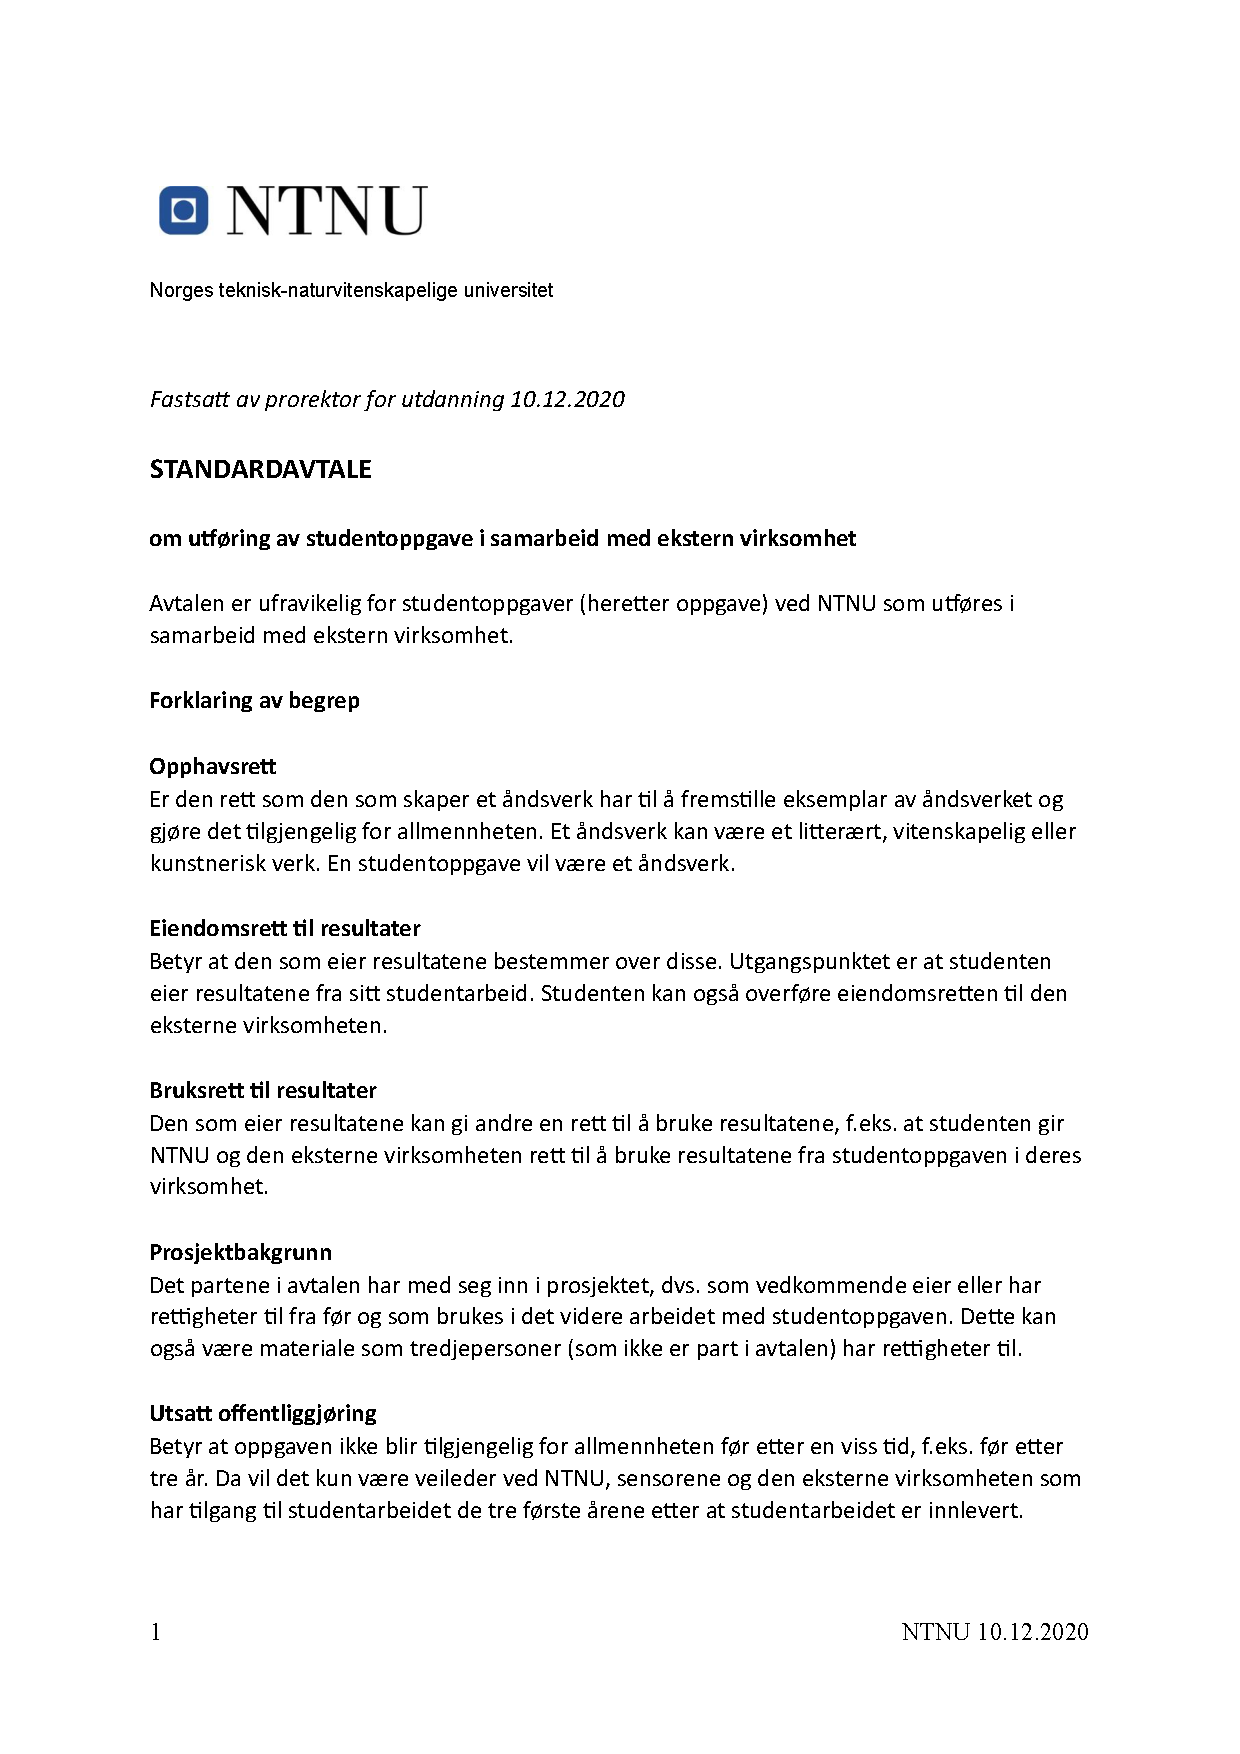
\includepdf[pages=-]{appendices/NTNUProsjektavtale.pdf}
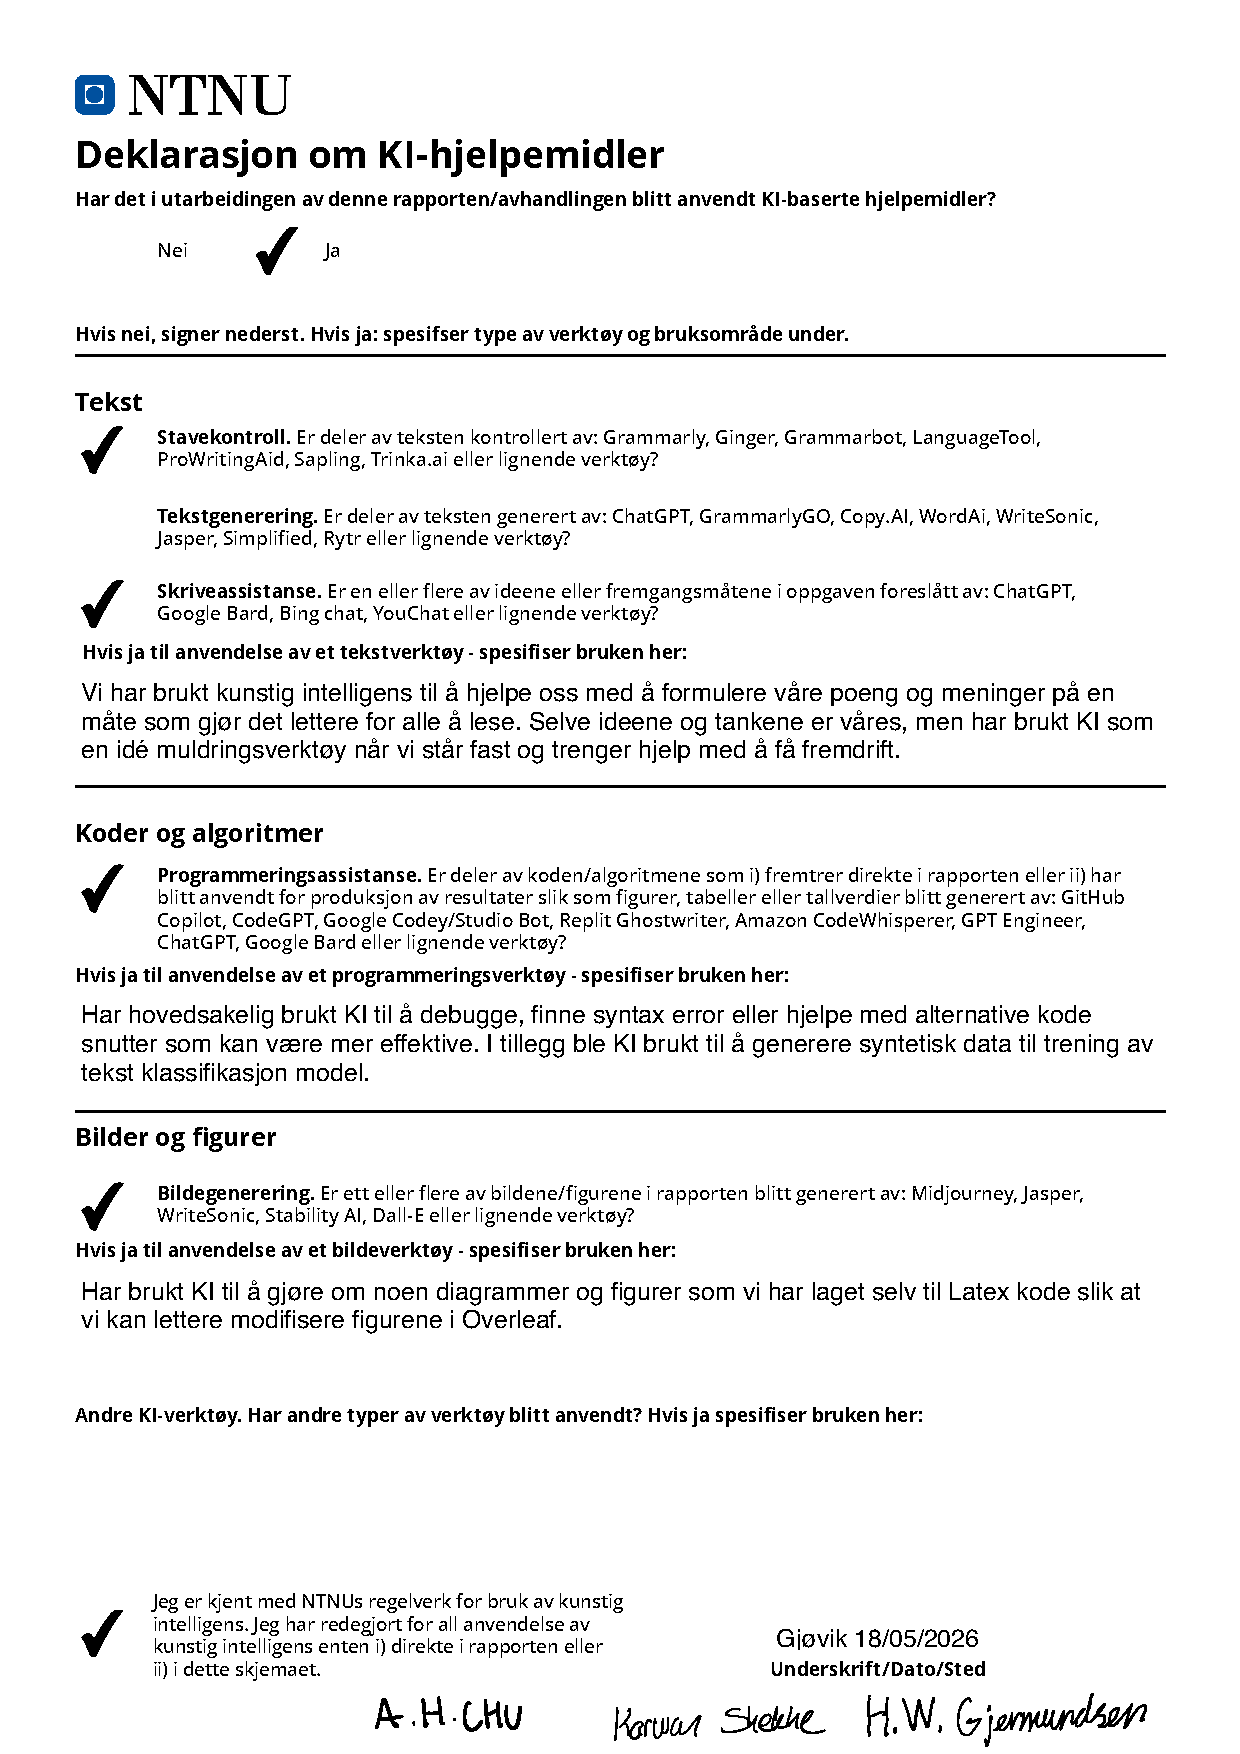
\includepdf[pages=-]{appendices/KI_Deklerasjon_BachelorV2026.pdf}
\chapter{Oppgave 37}
\label{app:oppgave37}

\section*{Assignment Information}

\begin{tabular}{@{}ll@{}}
\textbf{Assignment title:} & AI-based removal of sensitive information from images and video \\
\textbf{Company:} & Safe Media AI AS \\
\textbf{Contact person:} & Jon Yngve Hardeberg \\
\textbf{E-mail:} & jon@safemediaai.no \\
\textbf{Study program:} & DIGSEC, BIDATA, BPROG \\
\end{tabular}

\section*{Description}

Photographs and videos are widely used in society to document various locations and events. Examples include surveillance cameras, street view solutions from map providers, documentation of crime scenes, and journalistic photographs in public places. For privacy reasons, it is often necessary to remove sensitive information, such as recognizable faces, readable text, and metadata, from such photographs before they can be made publicly available. This process is sometimes called redacting, and doing it manually using tools such as Photoshop can be tedious and may also present several challenges. AI-based software solutions of various levels of quality are currently being proposed in the marketplace.

Safe Media AI AS has currently developed a powerful AI-based platform for redacting text-based documents. They would like to enhance their product portfolio by providing competitive solutions for redacting images and possibly videos. The overall goal of the project is to design, develop, and evaluate a complete and user-friendly solution for this, supported by state-of-the-art AI models.

\section*{Project Goals}

The project goals include:

\begin{itemize}
    \item Survey related state of the art from both research literature and available products.
    \item Develop a software solution which can identify and remove/redact sensitive content in images and videos.
    \item Ensure that the solution is compatible with existing tools developed by Safe Media AI AS, supports various file formats, and includes both fully automatic AI-based and user-friendly interactive methods.
    \item Ensure that the proposed solution is well justified with regards to state-of-the-art solutions, has a certain degree of novelty, follows strict standards for security and privacy, and is evaluated both quantitatively and qualitatively.
\end{itemize}

\chapter{In-depth User Interface and User Experience Design}
\label{app:depth_ui_ux}

This appendix provides additional documentation for the user interface design process described in Chapter~\ref{user_interface_and_usability}. While the main chapter focuses on the final interface and its usability principles, this appendix presents the earlier design iterations, prototype development, MVP stage, and additional interaction considerations that informed the final design.

\section{Design Methodology and Principles}

Development of the user interface followed an iterative design process, where layout, interaction patterns, and workflow structure were gradually refined throughout the project. Iterative design is widely recommended in user interface development because it allows teams to evaluate design decisions and improve solutions based on testing and practical experience \cite{hartson2012ux}. This approach allowed the design to evolve alongside the technical implementation while maintaining focus on usability and user control.

\methodheading{Iterative and Agile Design Process}

An agile development approach was used, where design and implementation were carried out in parallel. As new features were introduced, the interface was continuously adjusted to support the expanding functionality of the system. The approach aligns with Agile UX practices, where interface decisions are refined through incremental improvements rather than finalized early in development \cite{gothelf2022leanux}. 

Initial wireframes were created in Figma to explore layout and interaction flows before implementation (Appendix~\ref{fig:prototype_loaded}). Wireframing allows designers to quickly test ideas before committing to development \cite{hartson2012ux}. They were used to define the main workflow.

A functional prototype was then implemented to evaluate interaction patterns and identify usability issues in a practical environment. After the prototype stage, the design was refined into a minimum viable product (MVP), where core system functionality was integrated into the interface (Appendix~\ref{fig:mvp_detection}). The interface was also influenced by Safe Media AI's existing system, allowing users familiar with that platform to encounter recognizable layout structures and interaction patterns. This helped support consistency and reduced the learning curve for potential users.

\methodheading{Core Design Principles}

User control over automated processes was a central design principal. Since detection is performed by machine learning models, users must be able to verify, adjust, and override automated results when necessary \cite{hartson2012ux}. The interface supports this through manual highlighting, adjustment of detection settings, removal of incorrect detections, and customization of redaction methods.

Simplicity was also prioritized to reduce cognitive load and allow users to focus on identifying and redacting sensitive information \cite{norman2013design}. The interface therefore emphasizes essential functionality while avoiding unnecessary complexity. This was especially important because users must inspect visual content carefully and should not be distracted by unrelated interface elements.

Visual feedback was prioritized to help users understand system state and detection outcomes \cite{norman2013design}. Detection results are displayed directly on the media using labelled bounding boxes, enabling immediate interpretation of what the system has identified. Progress indicators and visible processing states further help users understand when the system is working.

Consistency across components improves usability and learnability \cite{nielsen2020progressive}. Toolbars, panels, and controls follow predictable patterns, making the interface easier to navigate. In addition, alignment with familiar structures from Safe Media AI's existing system supports recognition for users already accustomed to that platform, while still allowing SafeVision to introduce functionality specific to visual media redaction.

\section{Design Evolution}

The interface evolved through several stages, beginning with simple wireframes and later progressing into a prototype, MVP, and final interface. Each stage was used to explore layout, interaction flow, and the relationship between automated detection and manual user control.

The design was also influenced by Safe Media AI's existing interface. This was done to preserve familiar layout structures and interaction patterns for users already accustomed to that platform, while adapting the workflow to the specific needs of visual media redaction.

The early design stages focused on establishing the main workflow: uploading media, running detection, reviewing results, and applying redaction. Later iterations expanded this into a more complete workspace that supported manual correction, configuration options, visual feedback, and video processing.

\subsection{Initial Design}

Based on the initial requirements and project scope, the first interface design only needed to support a limited set of core functions: uploading an image, detecting sensitive information, and redacting detected content. Because of this limited scope, it was determined early in the design phase that the application did not require multiple pages, pop-up dialogs, or additional navigation views. Instead, the full workflow could be contained within a single interface, allowing users to complete the main redaction process in one place.

The initial interface was centered around a main interaction area for the uploaded image. Before upload, the interface presented a minimal layout with a central upload button, as shown in Figure~\ref{fig:prototype_empty}.

\begin{figure}[H]
\centering
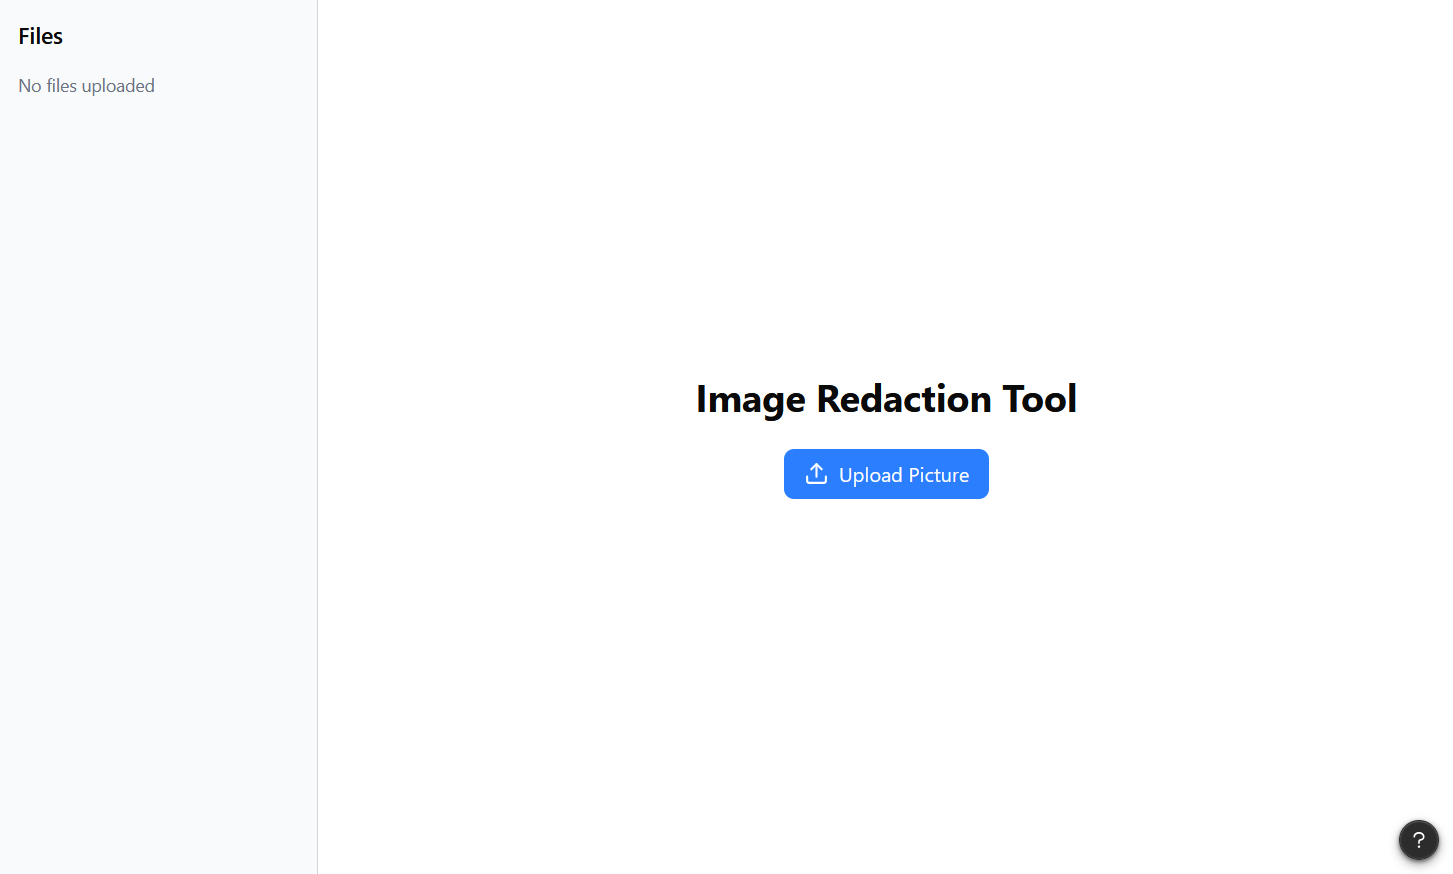
\includegraphics[width=0.8\textwidth]{figures/images/chapter-6/figmasketch3.png}
\caption{Initial interface before an image is uploaded.}
\label{fig:prototype_empty}
\end{figure}

After upload, the layout adapts to include interaction features. The upload button moves to the top, while the central area becomes the image viewer.

A file list is displayed on the left, and control buttons below the viewer allow detection, redaction, and highlighting. This placement maintains a clear connection between the image and available actions, as shown in Figure~\ref{fig:prototype_loaded}.

\begin{figure}[H]
\centering
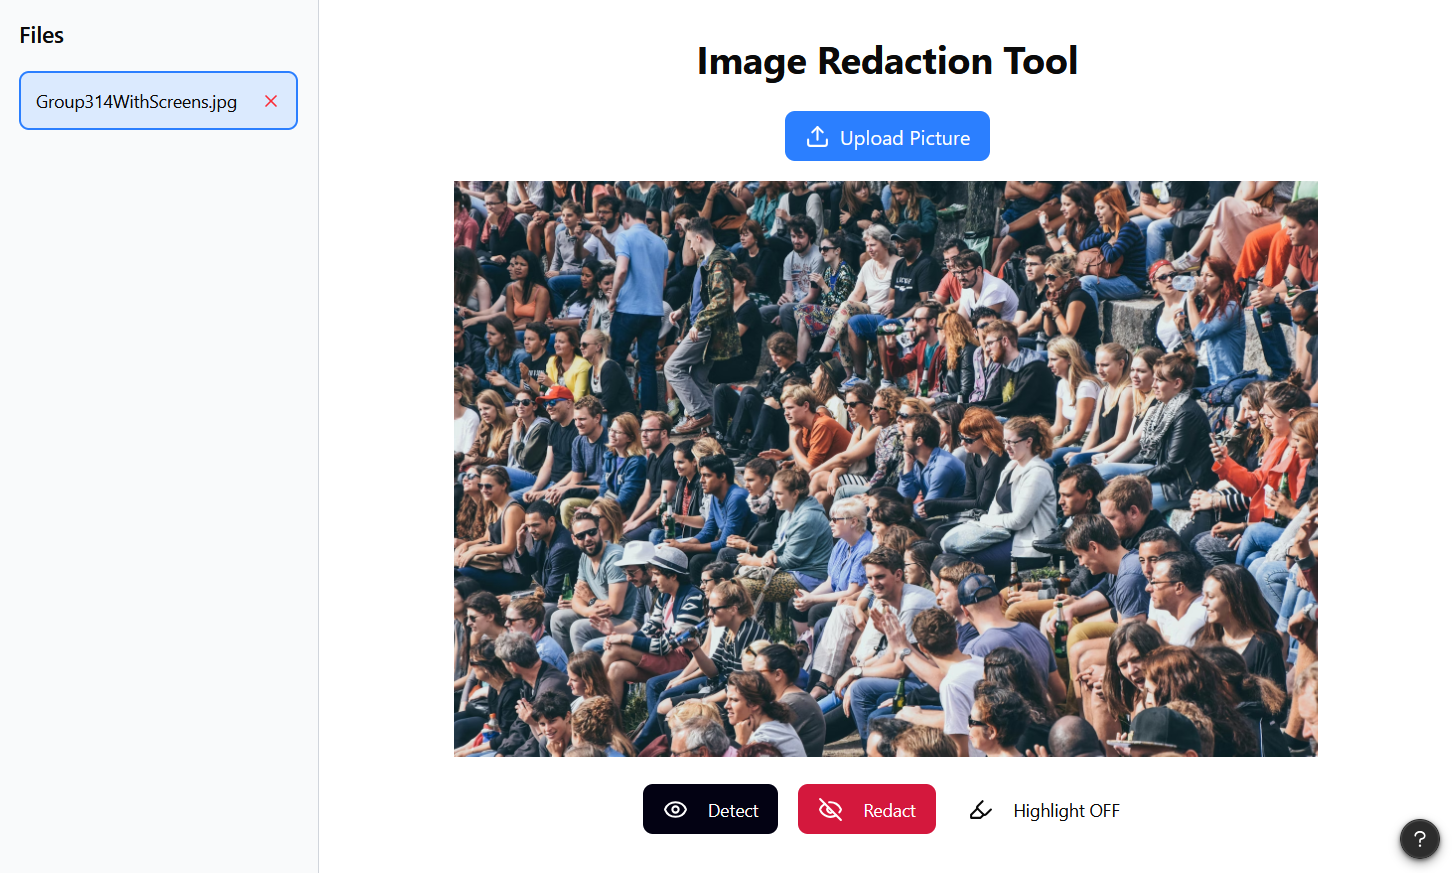
\includegraphics[width=0.8\textwidth]{figures/images/chapter-6/figmasketch4.png}
\caption{Prototype interface after an image has been uploaded.}
\label{fig:prototype_loaded}
\end{figure}

This design provides a clear workflow where users upload an image, run detection, and apply redaction.

\subsection{Prototype}

The prototype was developed in a separate repository to explore layout and interaction patterns without affecting the main system.

Key components such as a sidebar, navigation bar, and central viewer were introduced to structure the interface and organize available tools.

\begin{figure}[H]
\centering
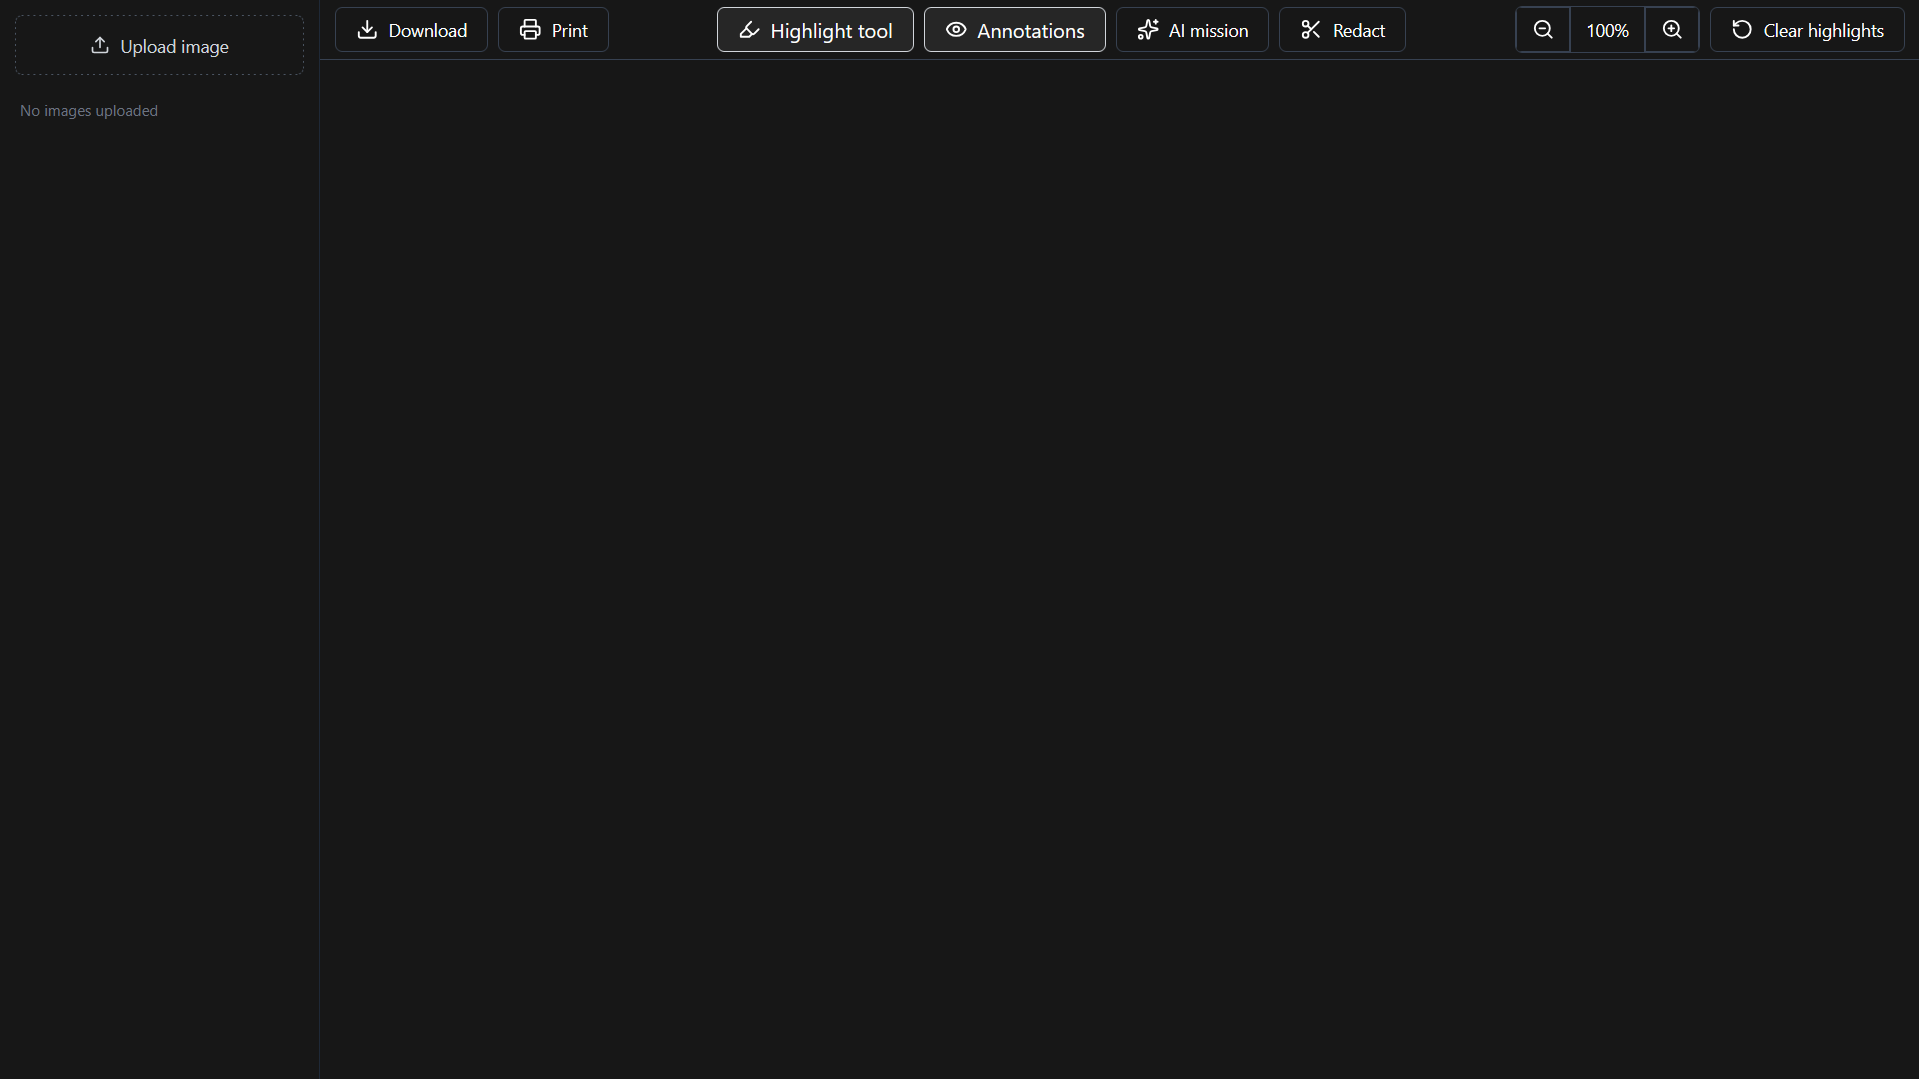
\includegraphics[width=0.8\textwidth]{figures/images/chapter-6/prototype1.png}
\caption{Prototype interface showing the sidebar, navigation bar, and image viewer.}
\label{fig:prototype_overview}
\end{figure}

Some elements were included for layout testing only, such as the \textit{AI Mission} and \textit{Redact} buttons.

The prototype also introduced manual highlighting, allowing users to mark regions directly within the viewer.

\begin{figure}[H]
\centering
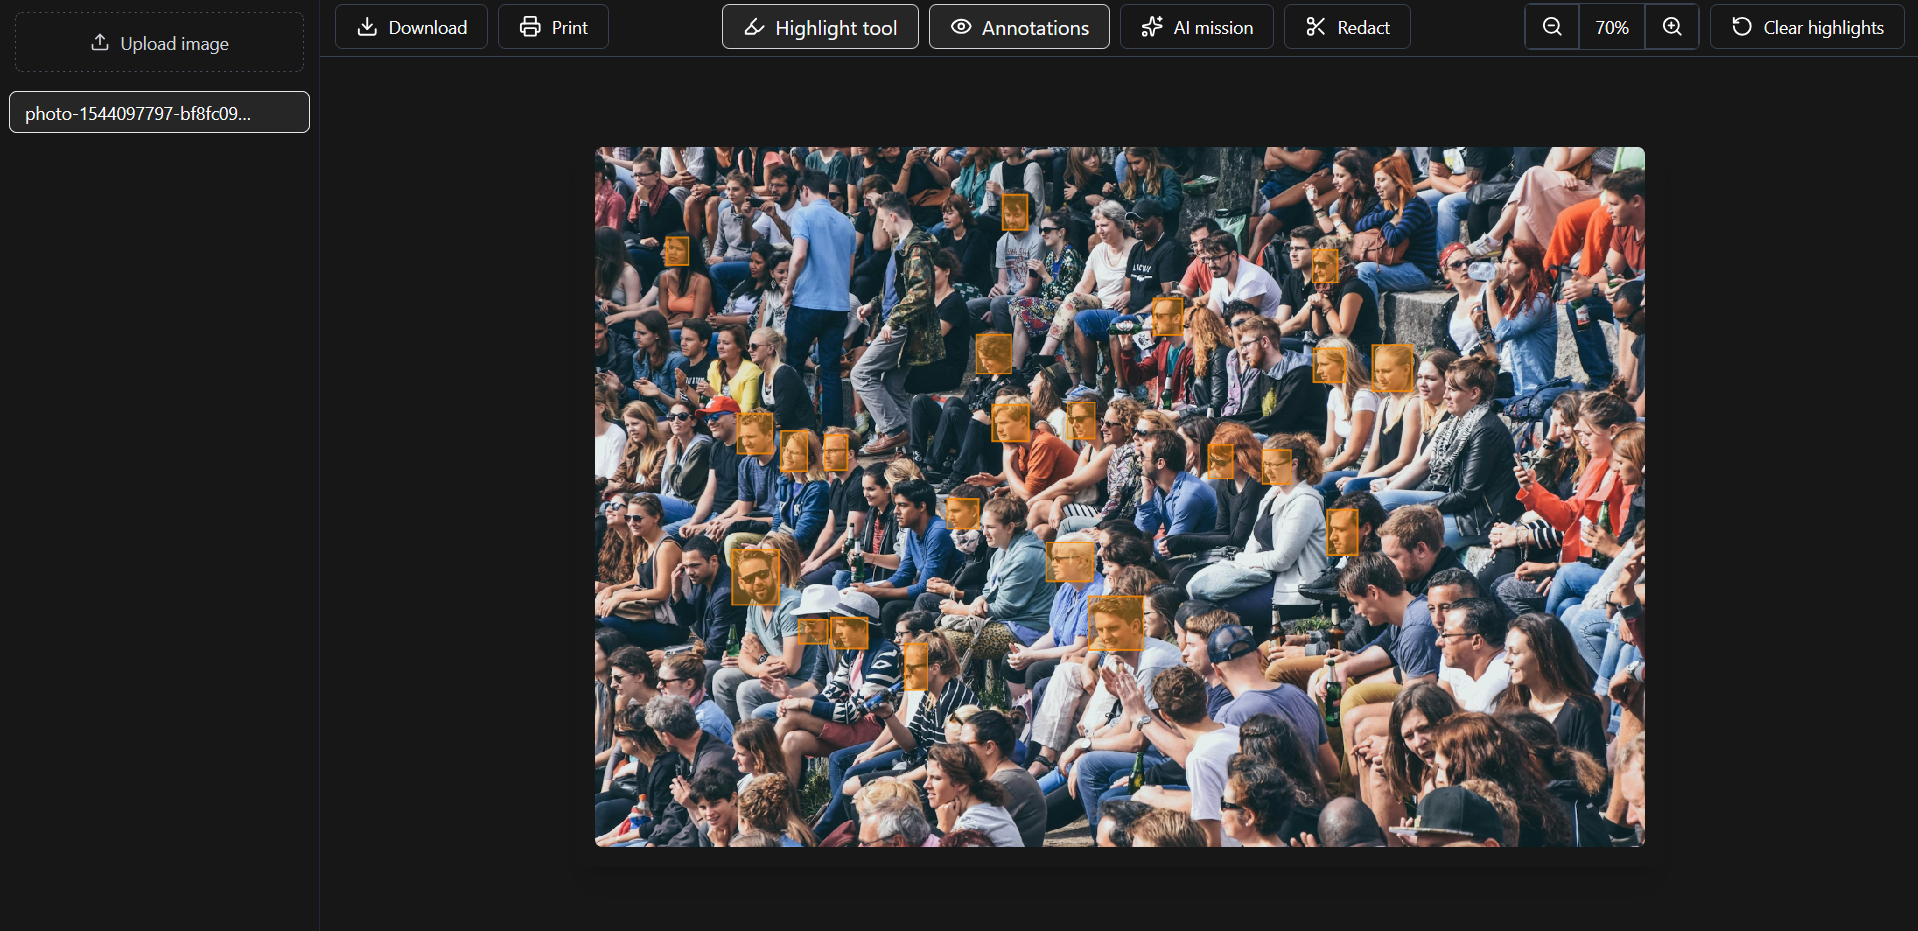
\includegraphics[width=0.7\textwidth]{figures/images/chapter-6/prototype3.png}
\caption{Prototype example showing manually highlighted regions.}
\label{fig:prototype_detection}
\end{figure}

\subsection{MVP Design Iteration}

The MVP introduced functional backend integration while preserving the basic prototype layout, including the sidebar structure and central viewer. Previously inactive interface elements were connected to system functionality, allowing users to run automatic detection and view results as bounding boxes.

At this stage, the interface also explored support for multi-page PDF documents. This allowed users to navigate pages within the same workspace. However, as the project scope evolved, PDF support became less central and the interface was later refocused around image and video redaction.

This iteration was important because it connected the visual interface to actual detection functionality. It also confirmed the need for a human-in-the-loop workflow, where automated detection results are shown visually and can be reviewed before redaction.

\begin{figure}[H]
\centering
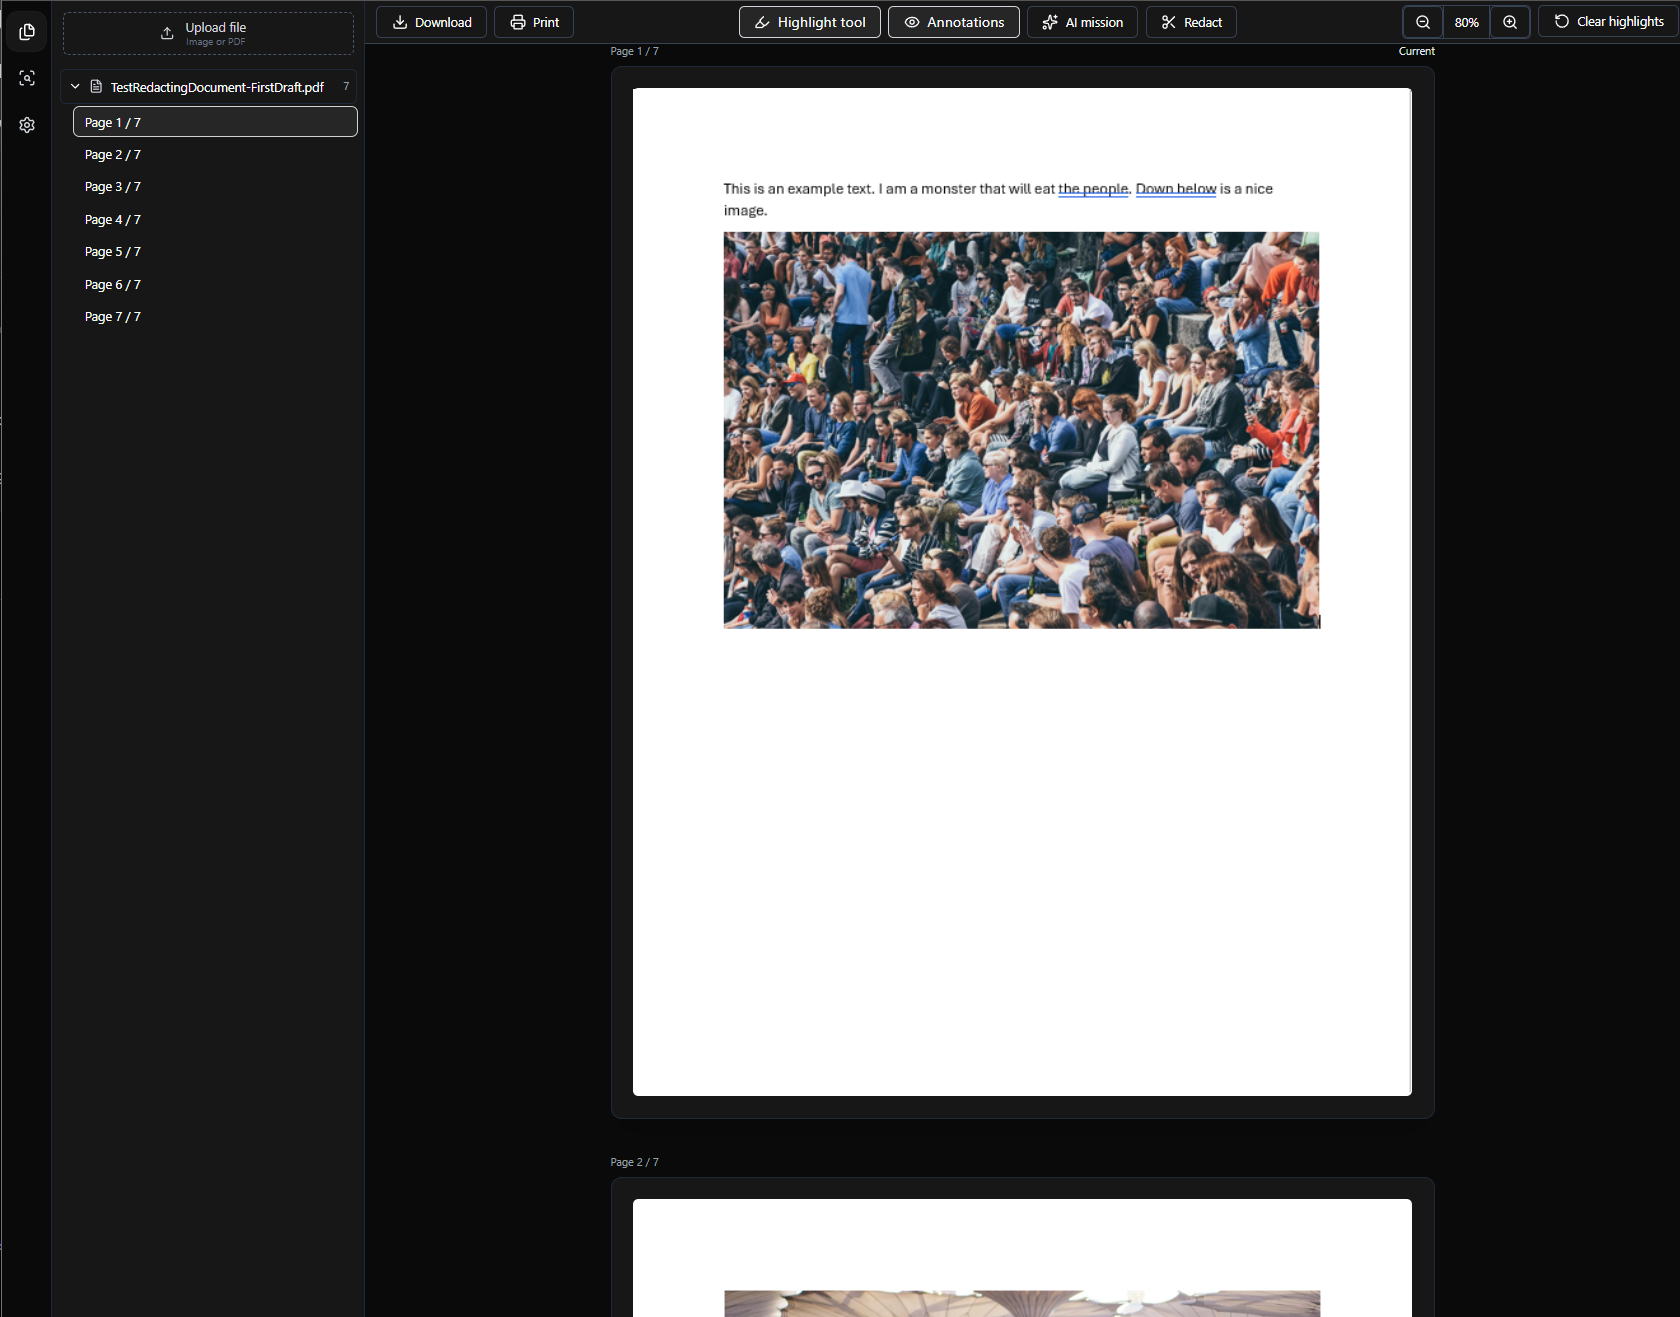
\includegraphics[width=0.8\textwidth]{figures/images/chapter-6/mvp1.png}
\caption{MVP interface showing the document viewer and navigation structure.}
\label{fig:mvp_overview}
\end{figure}

Support for multi-page PDF documents was also introduced, allowing users to navigate pages within the same interface.

\begin{figure}[H]
\centering
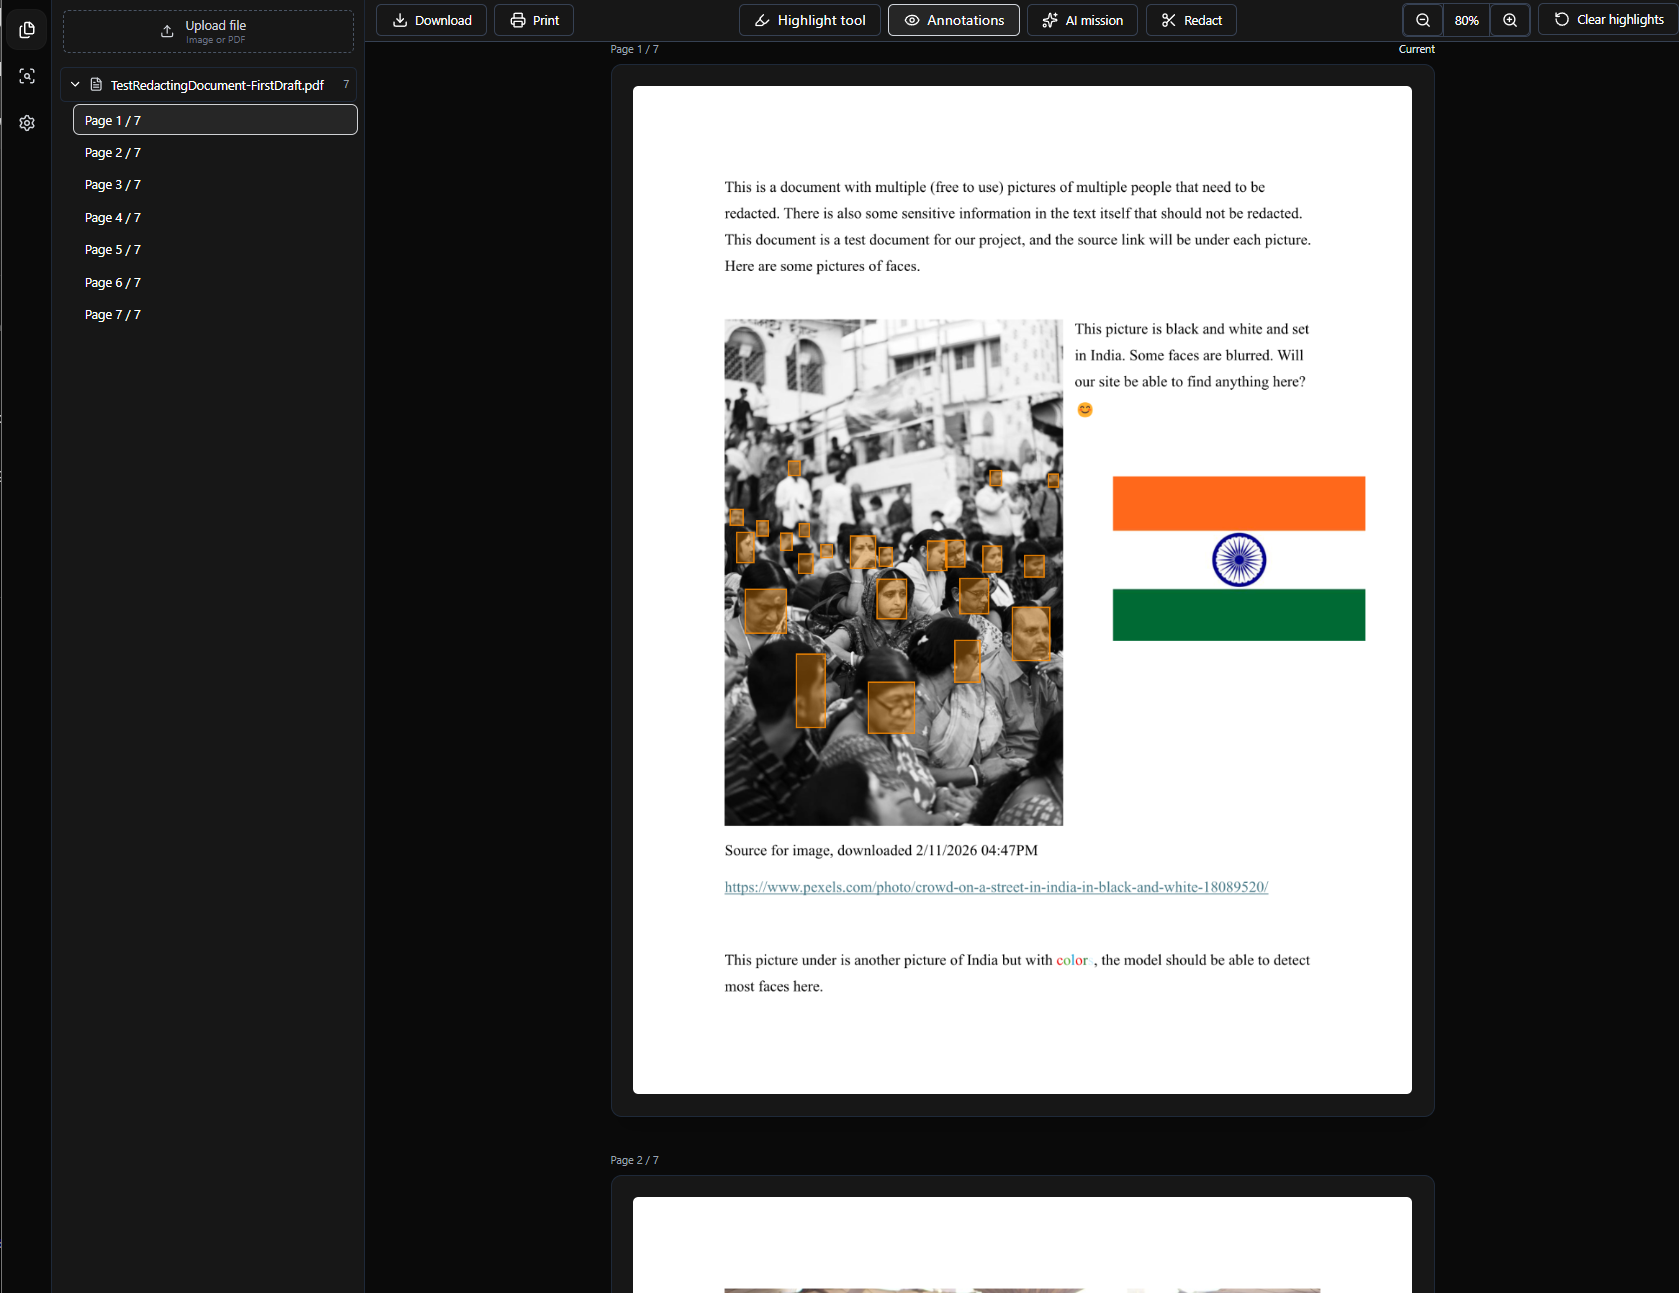
\includegraphics[width=0.8\textwidth]{figures/images/chapter-6/mvp2.png}
\caption{Detection results displayed using bounding boxes.}
\label{fig:mvp_detection}
\end{figure}

This iteration integrates automated detection with manual interaction, enabling users to verify and refine results before applying redaction.

\subsection{Final Design Direction}

The final design refined the interface into a focused workspace for image and video redaction. Compared with earlier iterations, the layout was simplified to reduce visual complexity and improve usability. The final interface retained the central viewer and side-panel structure, but reorganized controls so that upload, identification, review, correction, and redaction could be completed in a more natural sequence.

As the project evolved, support for PDF workflows was reduced, while video processing capabilities were introduced. This required the interface to support temporal media through playback controls, frame-based inspection, and detection overlays on video frames. A Terms of Service component was also implemented to address privacy and data protection requirements before users interact with the system.

The final interface and its components are described in the main text in Section~\ref{user_interface_and_usability}. This appendix therefore focuses on documenting the design progression that led to the final solution.

\section{Usability and Interaction Design}

This section focuses specifically on the interaction between the user and the machine learning-based detection and redaction functionality. While the interface includes several general usability features, the primary objective of the system is to support a human-in-the-loop workflow. Therefore, the usability discussion is centered on how users interact with detection results, verify automated outputs, and apply redaction.

\subsection{Interaction with Detection Results}

The core interaction in the system occurs within the document viewer, where detection results are presented directly on the image using bounding boxes. This allows users to immediately interpret the output of the detection models and understand which regions have been identified as potentially sensitive.

Since machine learning models are not perfectly accurate, it is essential that users can validate these results. The interface therefore allows users to manually adjust bounding boxes, remove incorrect detections, and add new regions if necessary. This ensures that the final outcome is not solely dependent on automated predictions, but can be refined through user input.

By combining automatic detection with manual correction, the system supports a more reliable and controllable redaction process.

\subsection{Detection Configuration and Control}

Users are able to control the detection process by selecting which categories of sensitive information to detect. This allows the system to be adapted to different use cases, where only specific types of content may be relevant.

Providing this level of control reduces unnecessary visual clutter and improves usability by ensuring that users only see relevant detection results. It also allows users to tailor the system behavior to the specific context of the document or image being processed.

\subsection{Redaction Interaction}

Once detection results have been reviewed, users can apply redaction directly within the interface. Multiple redaction methods are available, including black box redaction, blur, and pixelation.

Allowing users to select and adjust redaction methods provides flexibility in how sensitive information is concealed. For example, blur and pixelation may preserve some visual context, while solid redaction completely removes visibility. This enables users to choose the most appropriate method depending on the sensitivity of the content.

The integration of redaction controls within the same workspace as detection results ensures a seamless workflow, where users can move directly from analysis to action without changing context.

\subsection{Visual Feedback for Verification}

Clear visual feedback is essential when interacting with automated detection systems. In the interface, detection results are displayed as overlays on the document, allowing users to quickly assess model outputs.

This immediate feedback supports rapid verification, as users can visually confirm whether detected regions correspond to actual sensitive content. Any inaccuracies can then be corrected before redaction is applied.

By providing continuous visual feedback throughout the workflow, the interface helps users maintain awareness of system behavior and increases confidence in the final result.

\subsection{Accessibility Considerations}

Accessibility considerations were integrated into the interaction design to support effective use of detection and redaction tasks over extended periods. Since the system requires detailed visual inspection, emphasis was placed on reducing visual strain and enabling flexible interaction.

Visual accessibility is supported through dark and light modes, allowing adaptation to different lighting conditions. Users can also customize highlight colors for detection results and manual annotations, improving readability and distinction between detection categories. Zoom functionality further enables detailed inspection of small regions without losing context.

Interaction accessibility is addressed through flexible input methods. Keyboard shortcuts support efficient interaction during repetitive tasks, while undo and redo functionality allow users to safely adjust detection results and redaction without risk of permanent errors.

Together, these features improve usability, flexibility, and efficiency in the human-in-the-loop redaction workflow.

\methodheading{Terms of Services}
\label{app:terms_of_service}

A Terms of Service dialog was included in the final interface to clarify user responsibility, acceptable use, data handling, and the limitations of automated redaction. The text below summarizes the terms shown to users before processing content in \gls{SafeVision}.

\begin{enumerate}
    \item \textbf{Operator and contact:} The service is operated by An Hoang Chu, Karwan Shekhe, and Henrik Weflen Gjermundsen. Contact: henrik.w.gjermundsen@gmail.com.

    \item \textbf{What the service does:} The service provides automated detection and redaction functionality to help redact images. Automated detection may be inaccurate or incomplete.

    \item \textbf{User responsibilities and acceptable use:} Users confirm that they have the necessary rights and a valid legal basis to upload and process any personal data contained in the content they submit. Users must not upload unlawful content or content that infringes the rights or privacy of others. Users must not upload content involving children or other vulnerable individuals unless they are legally authorised to do so. Users are responsible for reviewing the output before sharing, publishing, or otherwise using it, because redaction may be imperfect. Access may be blocked or restricted if there is reasonable belief that the service is being misused or used unlawfully.

    \item \textbf{How images are processed, stored, and deleted:} When an image or document is uploaded, it is transmitted to the backend servers and processed by the system to detect sensitive content and apply redaction. The servers are hosted on infrastructure provided by Google Cloud. Uploaded images and redacted outputs are not stored permanently. Uploads are used only to generate the result and are deleted after the result is returned, although transient technical handling may occur during processing and delivery. Uploaded content is not used to train or improve the model.

    \item \textbf{Browser-stored backtracking and cached box data:} To support editing features, the web application stores derived detection data in the user's browser on the user's device. This may include bounding-box coordinates, image dimensions, and related redaction or editing state. The service uses an in-memory undo and redo history during the session, as well as local browser storage or cache to restore detected boxes and editing state when the user revisits the site. This browser-stored data does not include the original uploaded image. Users can remove this data at any time by clearing the site's data in their browser.

    \item \textbf{Logging:} The service does not intentionally log or retain uploaded image content. Some infrastructure-level operational data may be processed transiently to deliver the service.

    \item \textbf{Rights and complaints:} For questions or data protection requests, users can contact henrik.w.gjermundsen@gmail.com. Users may also lodge a complaint with their supervisory authority, Datatilsynet.

    \item \textbf{Disclaimer:} The service is provided ``as is'' and ``as available.'' The system does not guarantee that all sensitive content will be detected or redacted. Users are responsible for verifying outputs before sharing or publishing. Nothing in these terms limits liability where such limitation is not permitted by law.
\end{enumerate}



% appendices/custom_detection_model_evaluation.tex

\chapter{Detailed Evaluation of Custom-Trained Detection Models}
\label{app:custom_model_evaluation}

\section{Barcode Detection}
\label{app:barcode_detection}
This section provides detailed training and evaluation results for the final
barcode detection model.

\subsection{Training Setup}

\begin{table}[H]
\centering
\begin{tabular}{lccc}
\toprule
Total Images & Training & Validation & Testing \\
\midrule
15731 & 12583 & 1572 & 1576 \\
\bottomrule
\end{tabular}
\caption{Dataset split used for the barcode detection model.}
\label{tab:bc_training_split}
\end{table}

\subsection{Training Configuration}

\begin{table}[H]
\centering
\caption{Training configuration for the final barcode detection model.}
\label{tab:barcode_training_config}
\scriptsize
\renewcommand{\arraystretch}{1.05}
\begin{tabular}{lp{7cm}}
\toprule
\textbf{Parameter} & \textbf{Value} \\
\midrule
Architecture & YOLOX-S \\
Input Resolution & $960 \times 960$ \\
Batch Size & 4 \\
Max Epochs & 150 \\
No-Aug. Epochs & 15 \\
\midrule
\textit{Optimization} & \\
Base Learning Rate & 0.01 / 64 \\
Warmup Epochs & 5 \\
Min LR Ratio & 0.05 \\
Optimizer & SGD \\
\midrule
\textit{Augmentation} & \\
Mosaic / Mixup & 0.0 / 0.0 \\
Color / Flip & 0.5 / 0.5 \\
Rotation / Shift / Shear & 5.0 / 0.05 / 1.0 \\
\midrule
\textit{Hardware} & \\
GPU Model & RTX 4080 \\
\bottomrule
\end{tabular}
\end{table}







\subsection{Training Behaviour}

\begin{figure}[H]
\centering

\begin{subfigure}{0.50\textwidth}
\centering
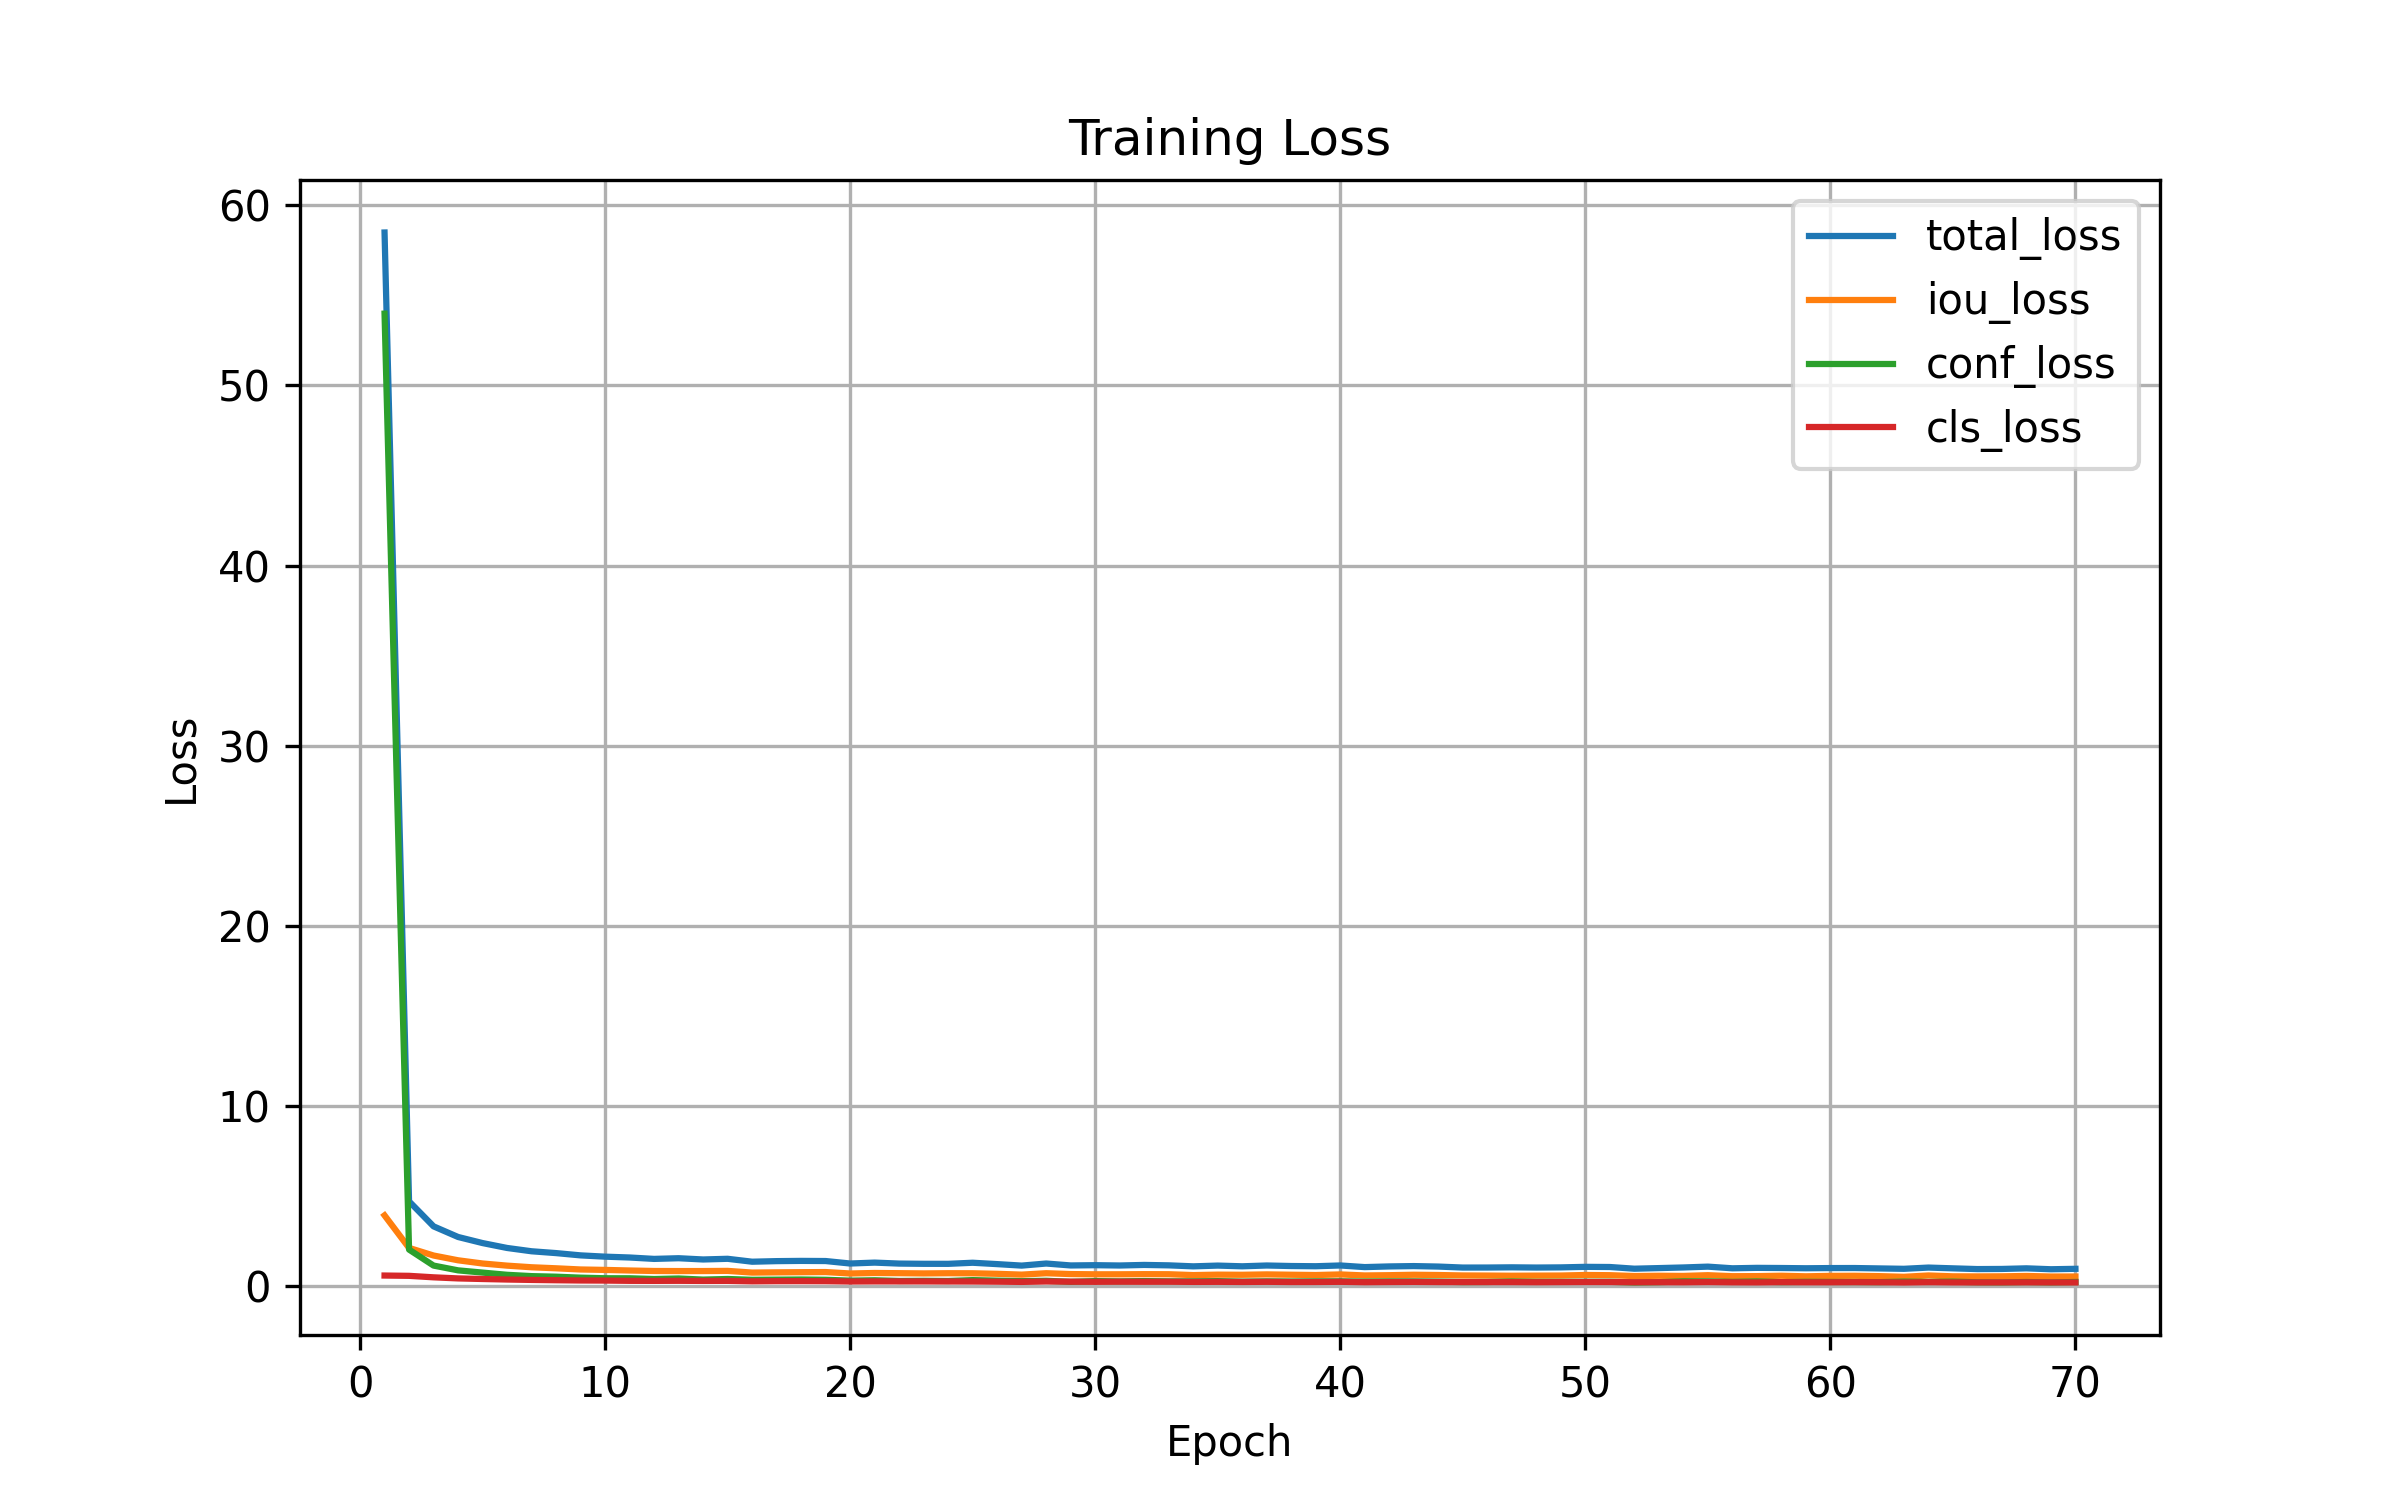
\includegraphics[width=\linewidth]{figures/images/chapter-11/qr-bar/v0/loss_curve.png}
\caption{Training loss}
\end{subfigure}
\hfill
\begin{subfigure}{0.48\textwidth}
\centering
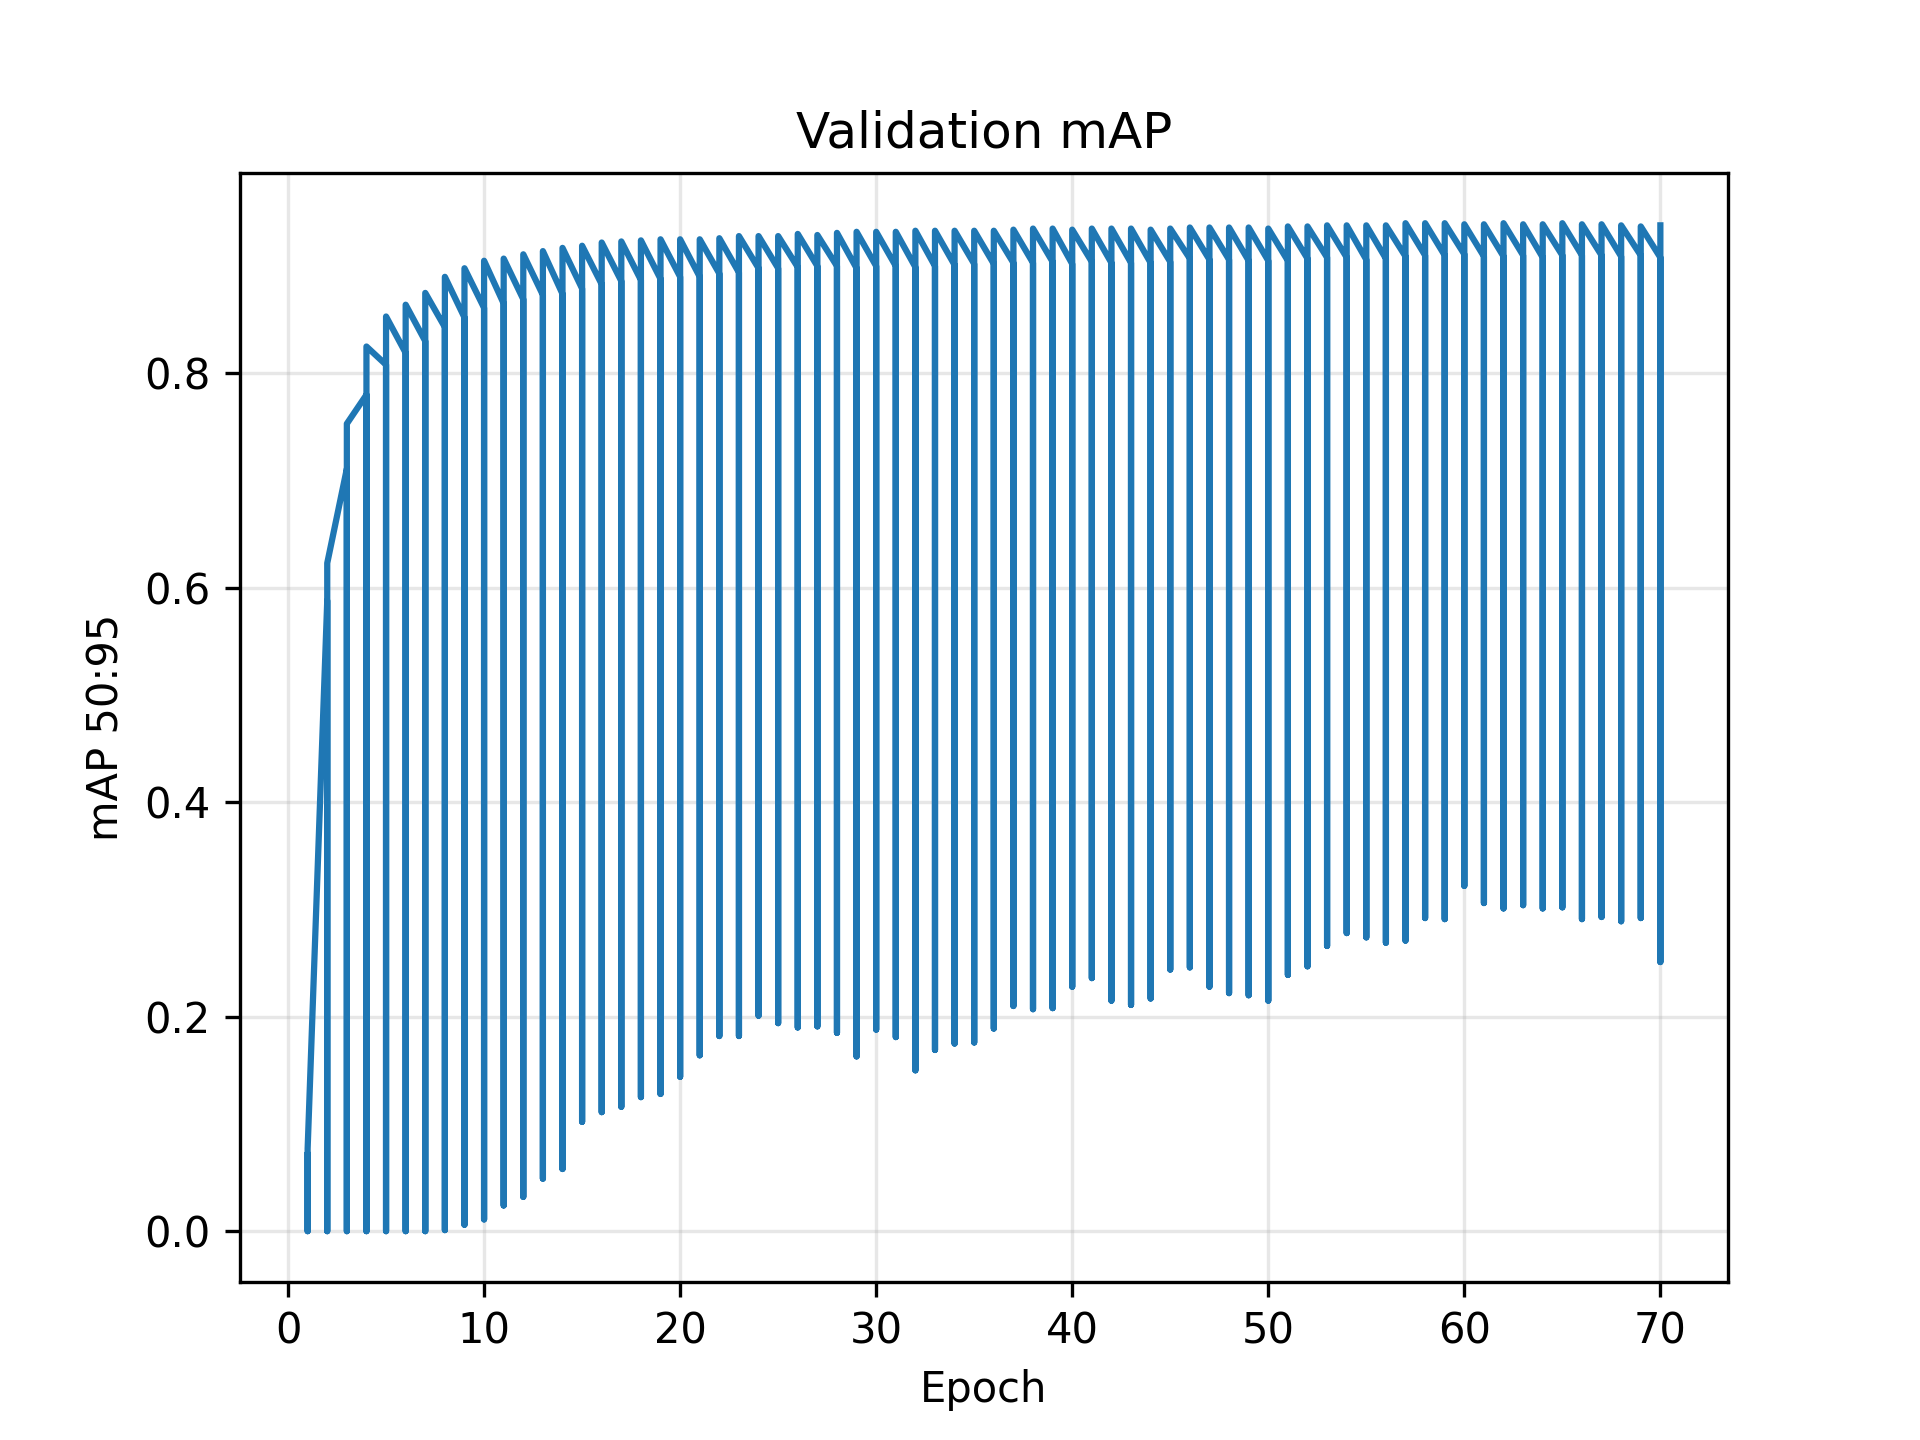
\includegraphics[width=\linewidth]{figures/images/chapter-11/qr-bar/v0/map_curve.png}
\caption{Validation mAP}
\end{subfigure}

\vspace{0.4cm}

\begin{subfigure}{0.50\textwidth}
\centering
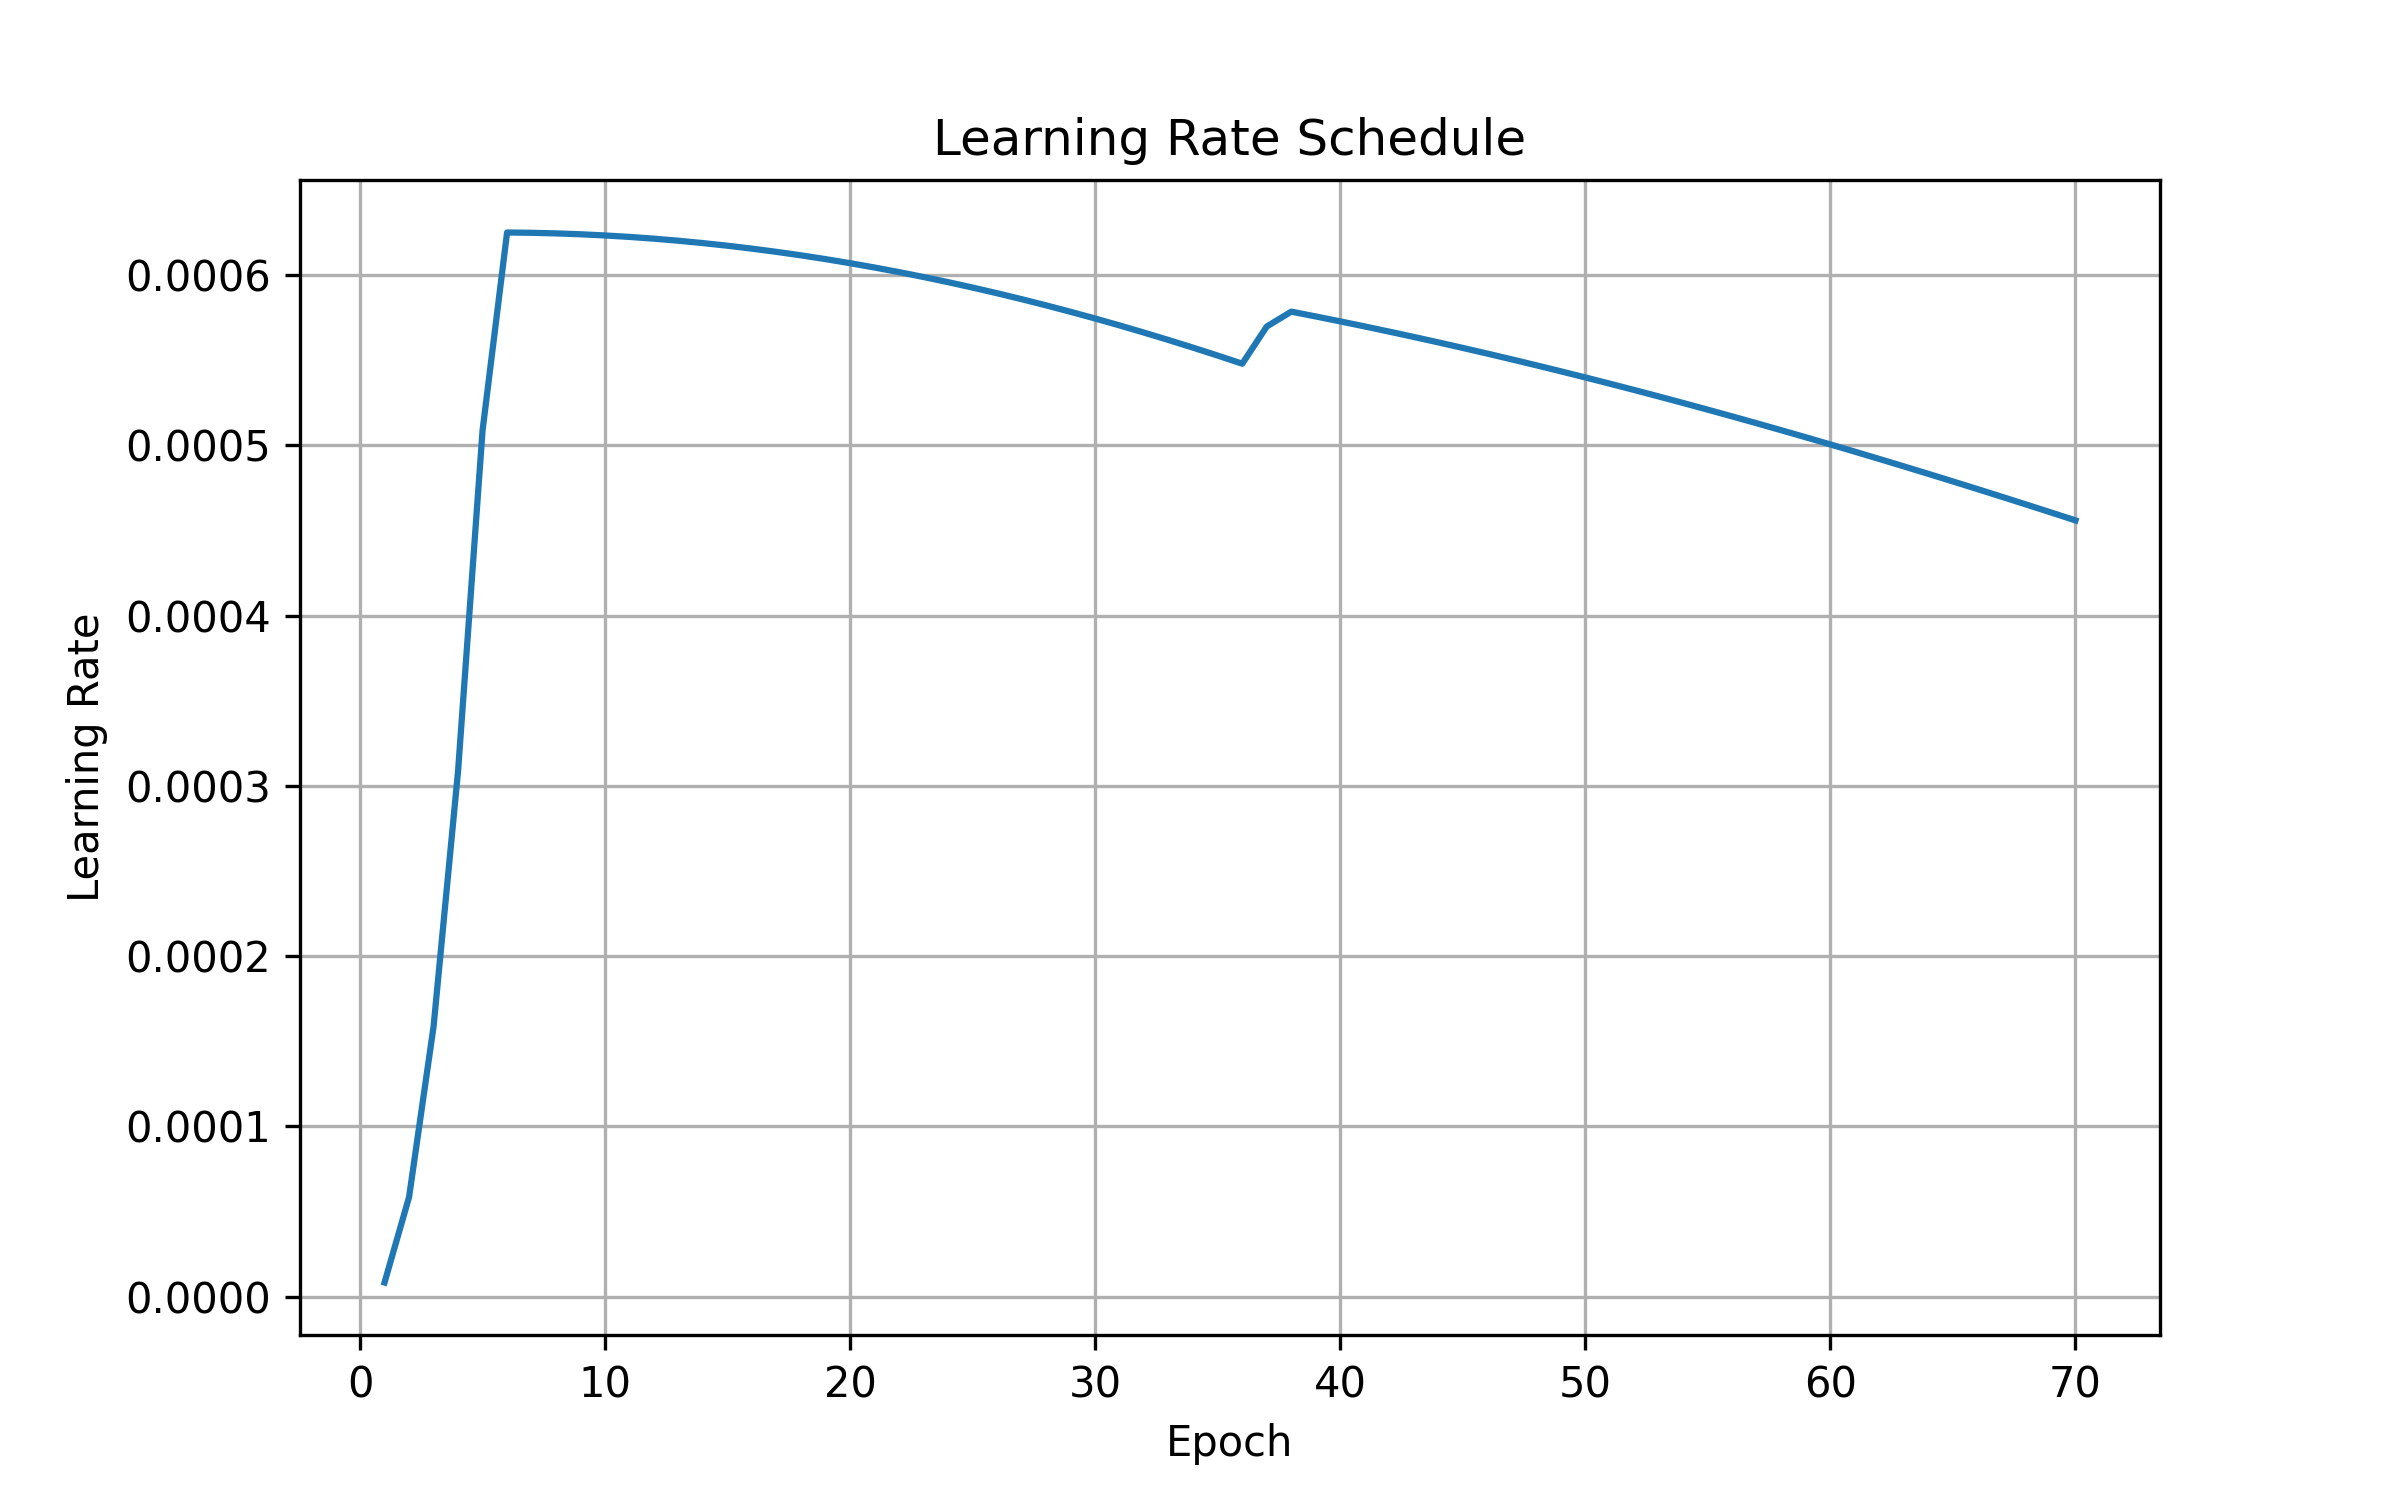
\includegraphics[width=\linewidth]{figures/images/chapter-11/qr-bar/v0/lr_curve.png}
\caption{Learning rate schedule}
\end{subfigure}

\caption{Training behaviour of the final barcode detection model.}
\label{fig:bc_training}
\end{figure}

The training loss decreases rapidly during the initial epochs and gradually
stabilizes, indicating successful convergence of the model.

The validation mAP increases quickly and stabilizes at a high level, showing
that the model generalizes well to unseen data.



\subsection{Precision--Recall Analysis}

\begin{figure}[H]
\centering
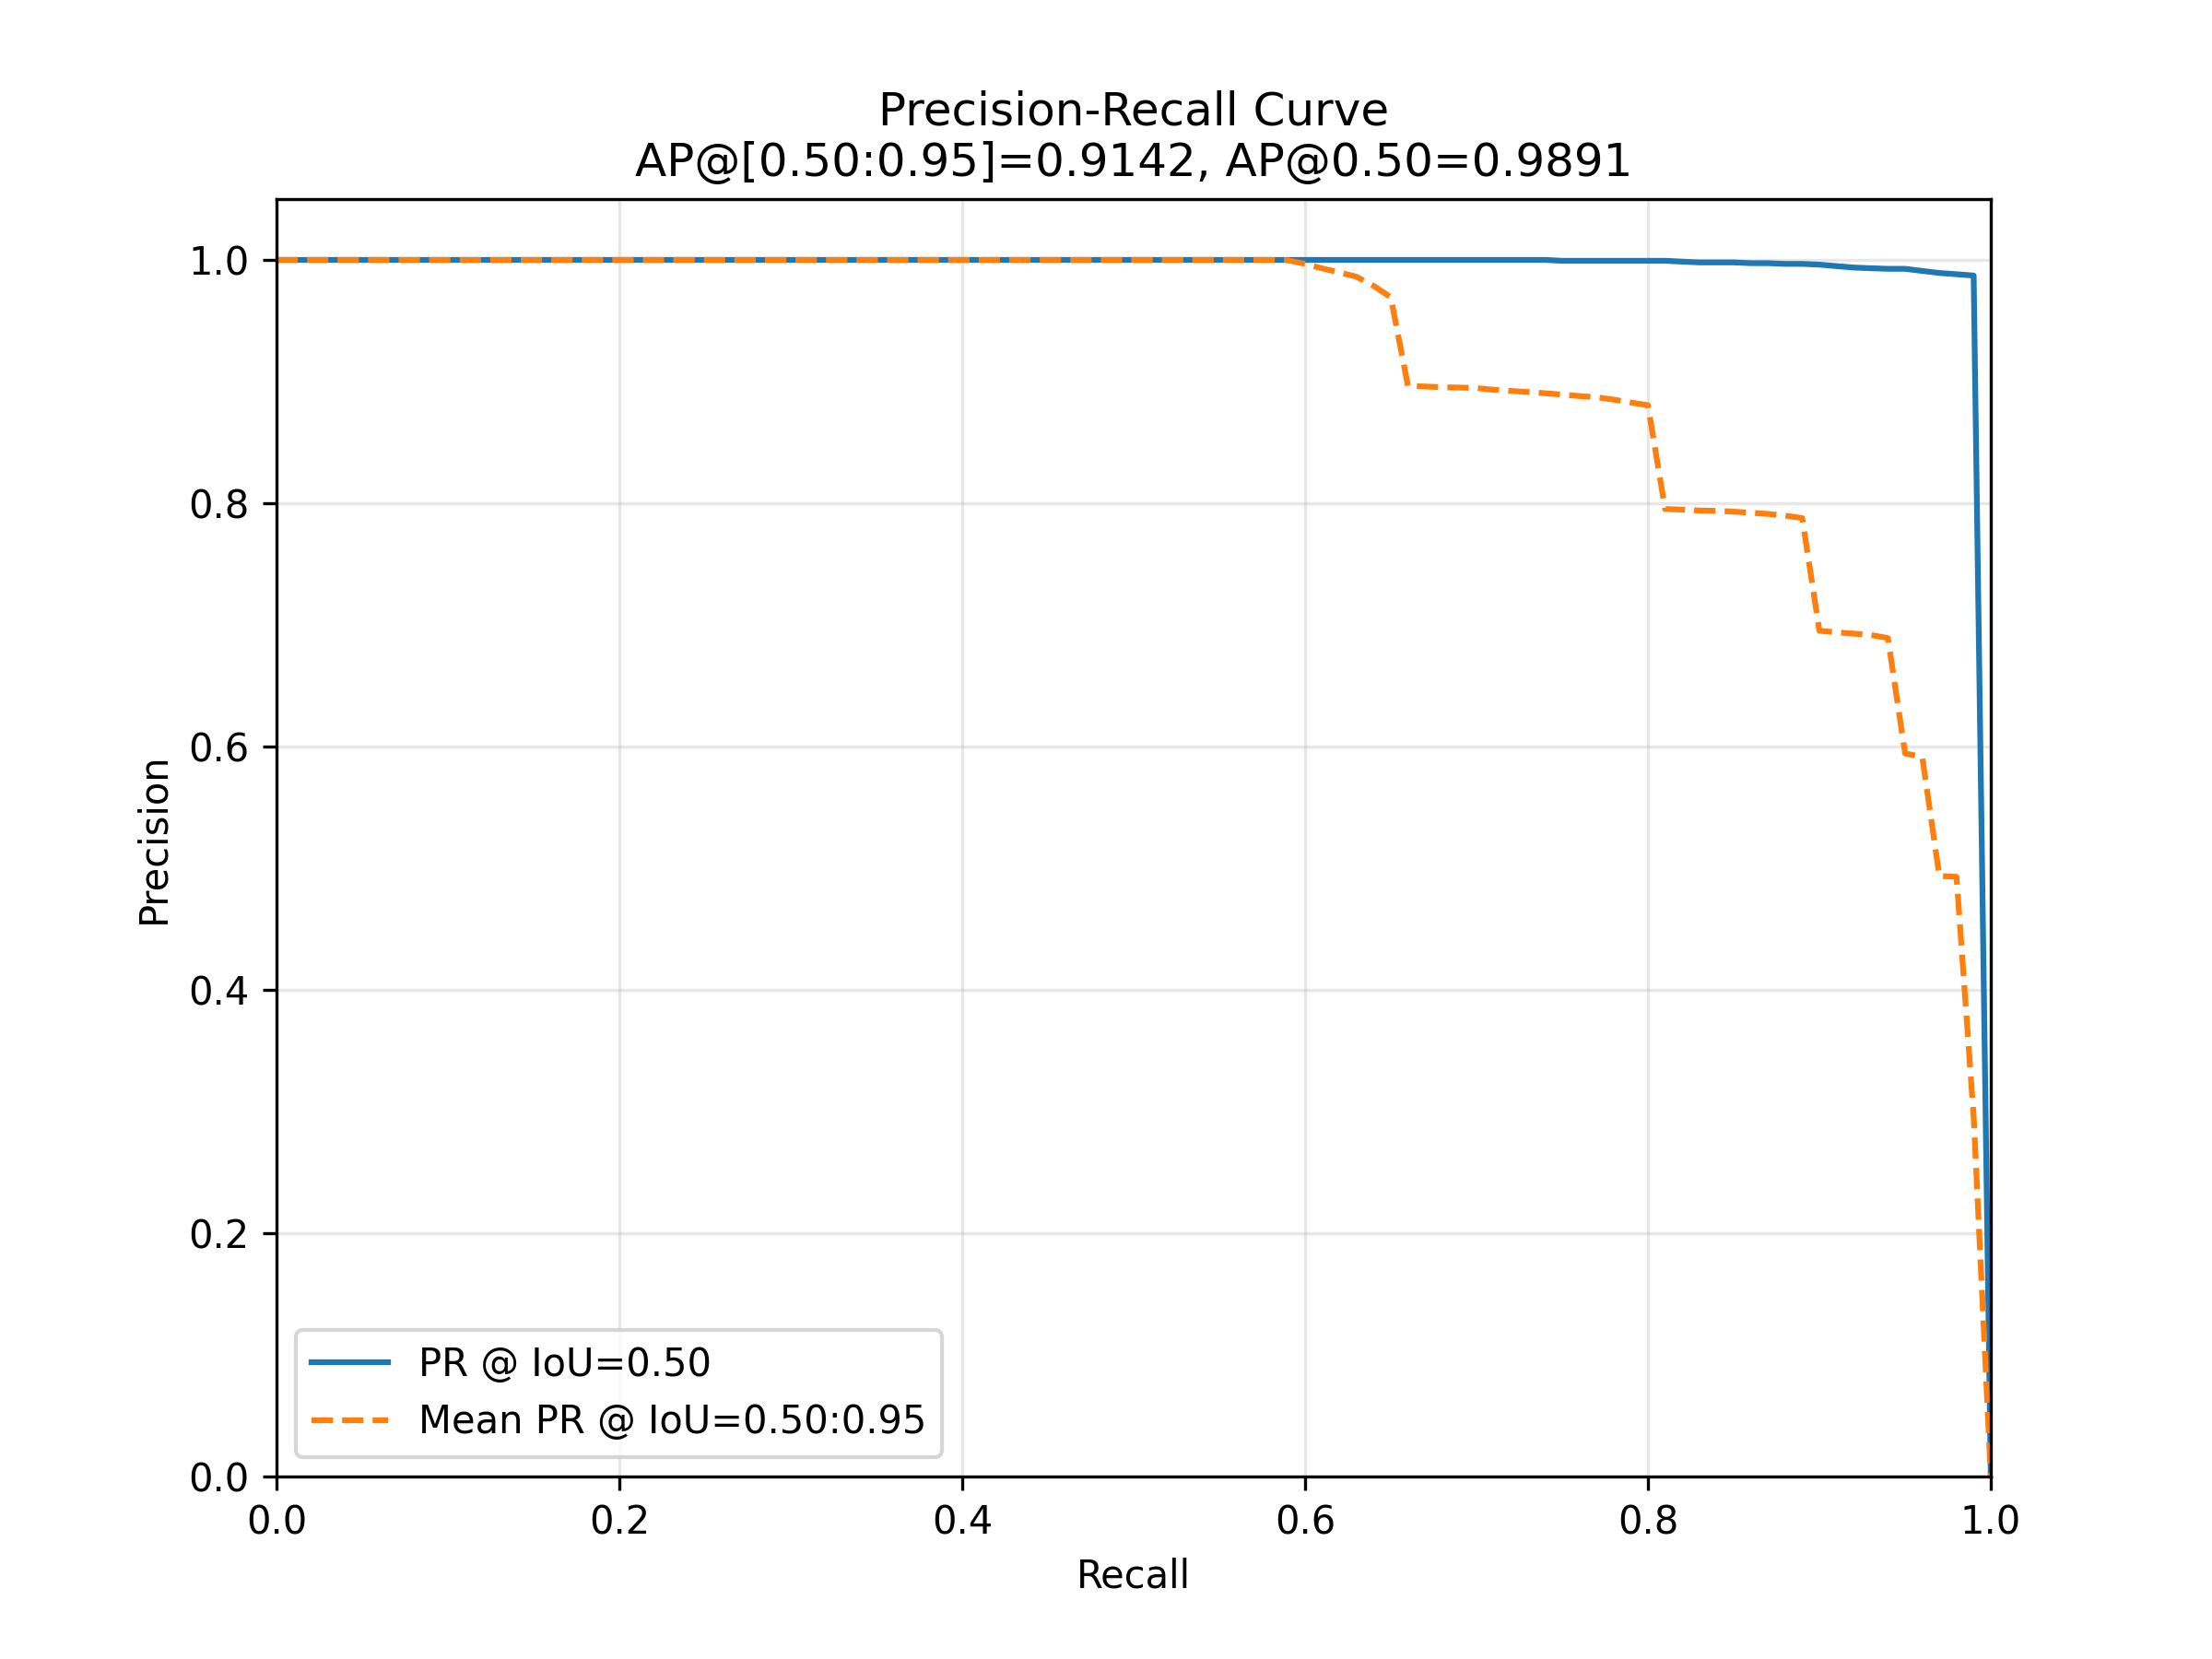
\includegraphics[width=10cm]{figures/images/chapter-11/qr-bar/v0/pr_curve.png}
\caption{Precision--recall curve for the barcode detection model.}
\label{fig:bc_pr_curve}
\end{figure}

The model achieves a high Average Precision, with
$AP@0.50 = 0.989$ and $AP@0.50:0.95 \approx 0.91$,
indicating strong detection performance across different IoU thresholds.




\subsection{Confusion Matrix Analysis}

\begin{figure}[H]
\centering
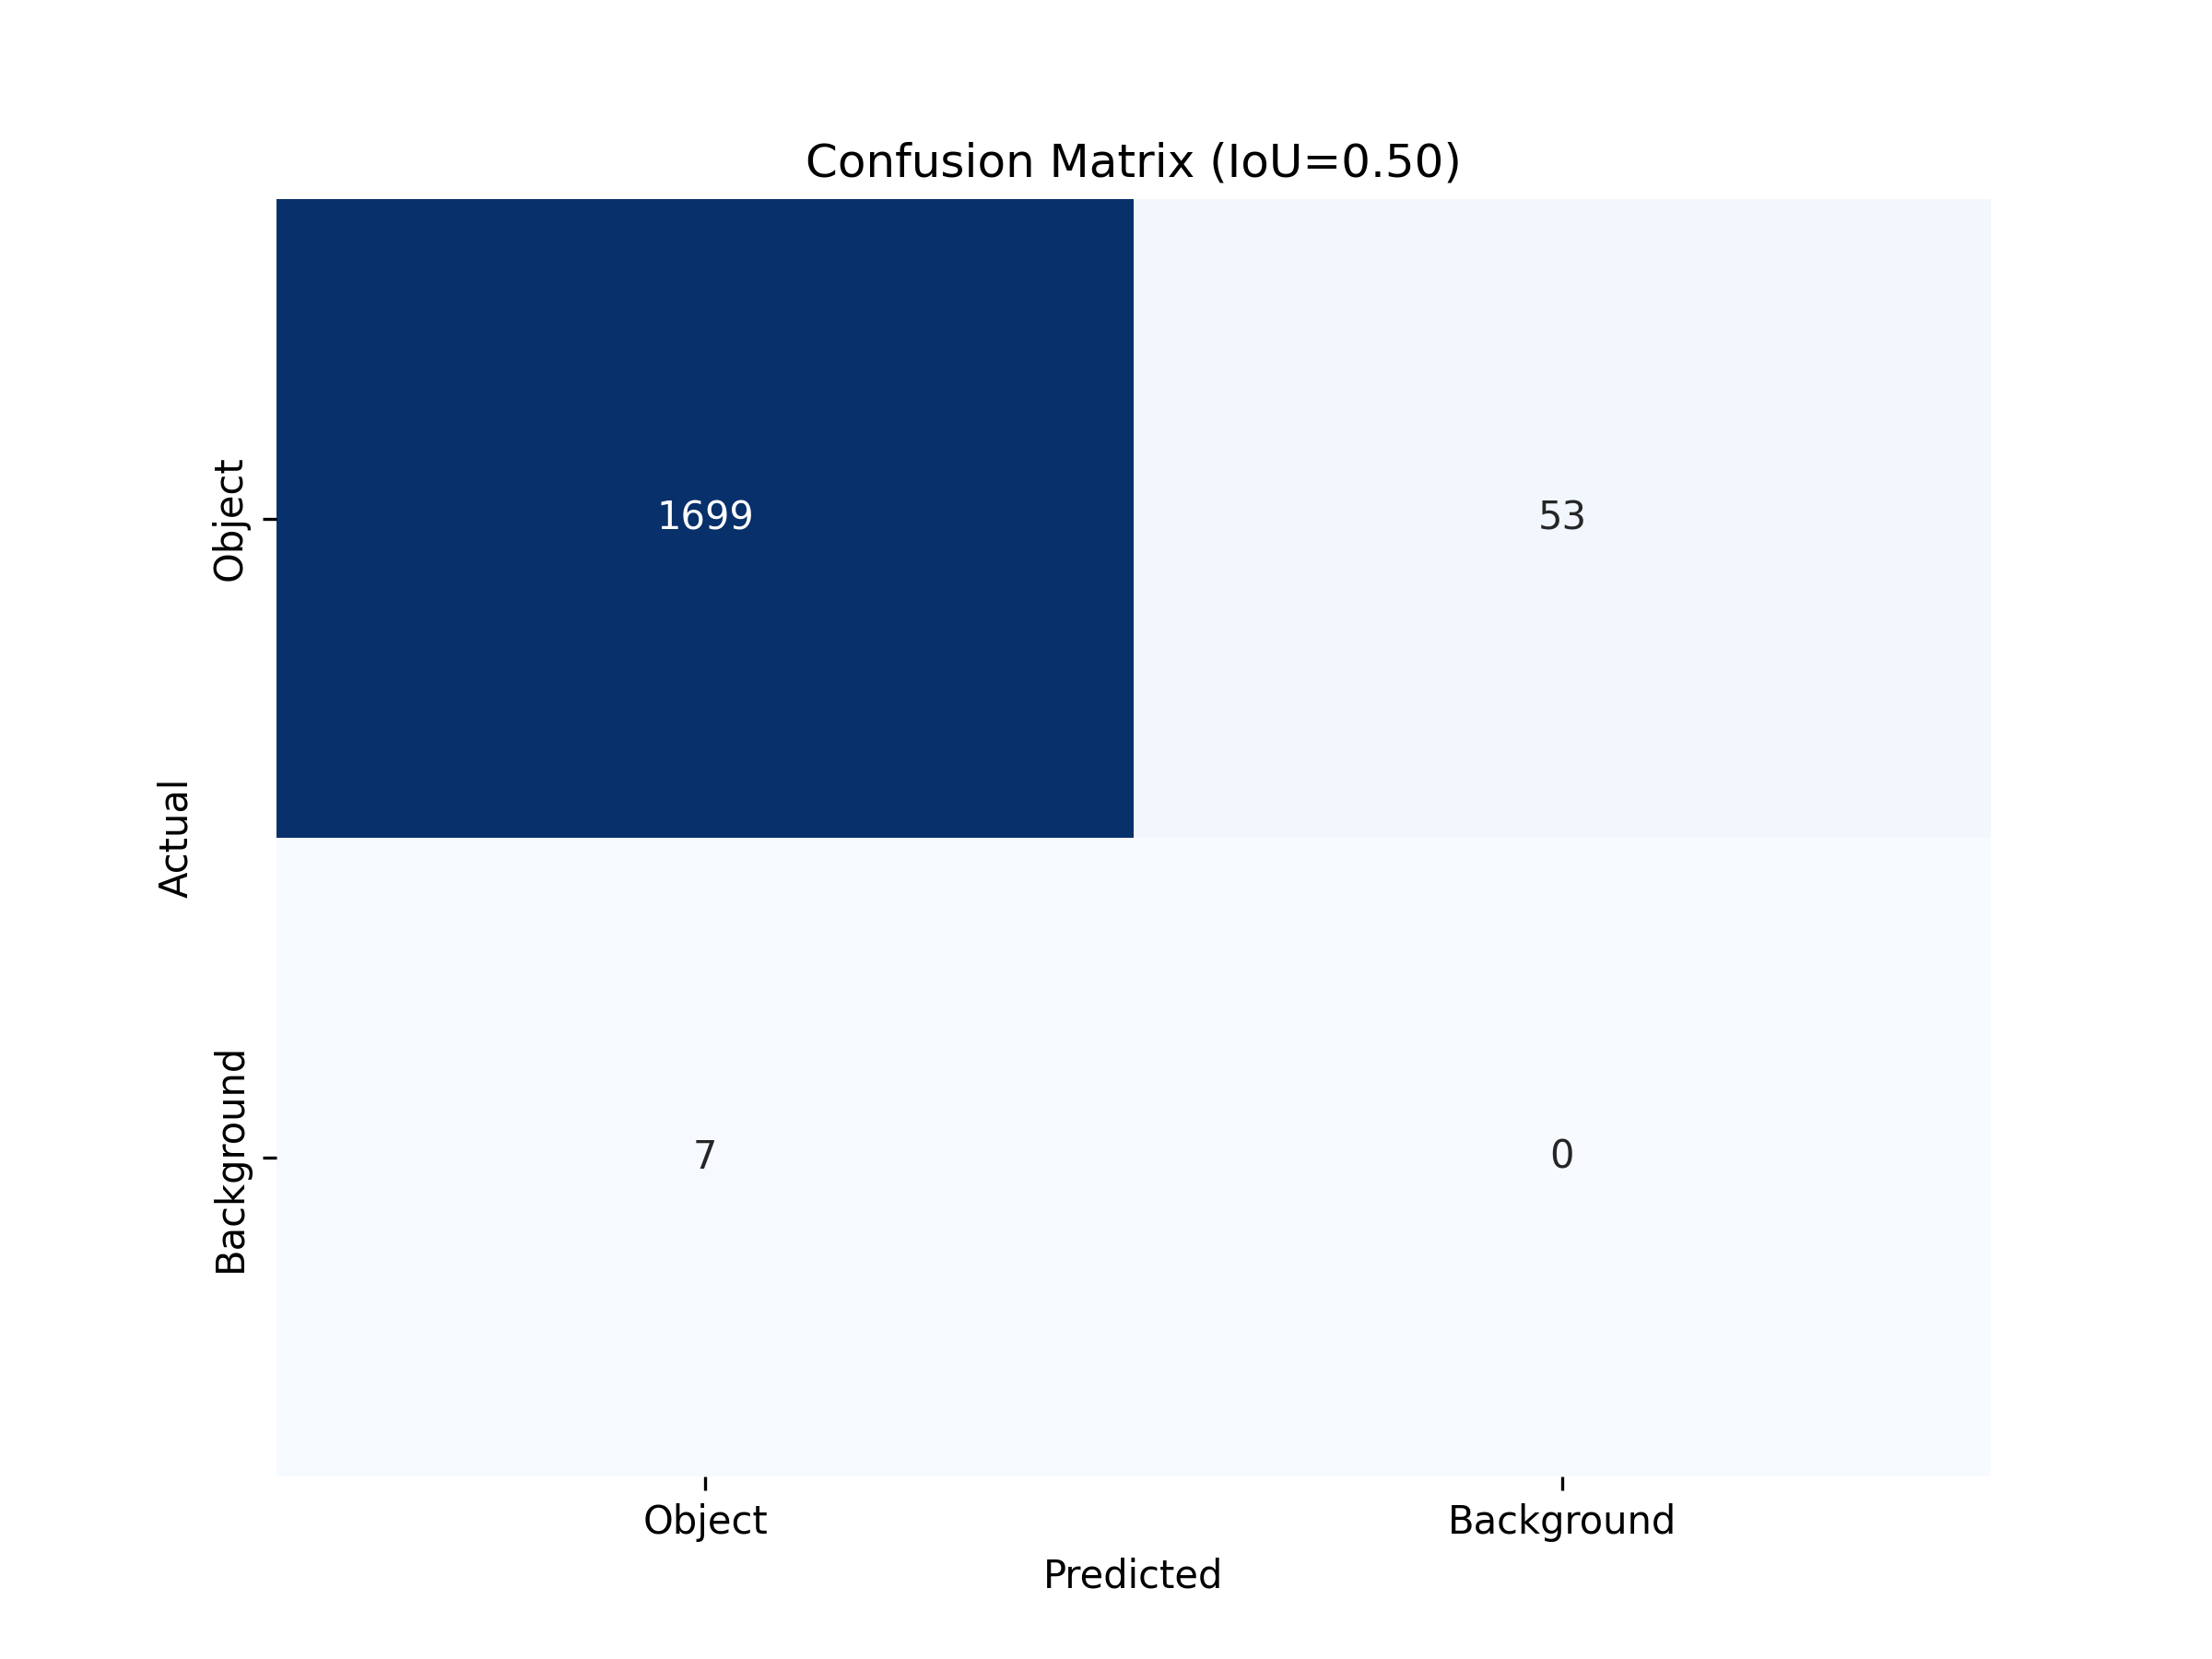
\includegraphics[width=12cm]{figures/images/chapter-11/qr-bar/v0/confusion_matrix_0.3.png}
\caption{Confusion matrix for the barcode detection model.}
\label{fig:bc_confusion_matrix}
\end{figure}

The model correctly detected 1699 barcodes, produced 53 false positives,
and missed 7 barcodes.

\begin{align*}
Precision &= \frac{1699}{1699 + 53} \approx 0.9697 \\
Recall &= \frac{1699}{1699 + 7} \approx 0.9959 \\
F1 &= 0.983
\end{align*}

\subsection{Summary}

The final barcode detection model achieved strong performance on the unseen
test set. At a confidence threshold of 0.3, the model obtained a precision of
96.97\%, a recall of 99.59\%, and an F1-score of 0.983.

The high recall indicates that the model missed very few barcodes, while the
high precision shows that most predicted detections were correct. Combined with
the high Average Precision values, these results indicate that the barcode
detector is suitable for use in the proposed system.






% ------------------------------------------------------------------------


\section{License Plate Detection}
\label{app:license_plate_results}

This section documents the detailed training and evaluation results for the
custom-trained license plate detection models. The model was trained using the
same YOLOX-based training pipeline as the barcode detection model. Therefore,
this section focuses on the supporting results used to evaluate and compare the
license plate detector configurations.


\subsection{Training Setup}

\begin{table}[H]
\centering
\begin{tabular}{l l p{5.0cm}}
\toprule
\textbf{Dataset} & \textbf{Source} & \textbf{Description} \\
\midrule
License Plate Detection Dataset
& Kaggle \cite{lp_dataset_1} 
& Dataset containing annotated license plate images from real-world environments, designed for object detection tasks \\

Large License Plate Detection Dataset
& Kaggle \cite{lp_dataset_2} 
& Large-scale dataset with diverse license plate instances captured under varying lighting and environmental conditions \\

\midrule
\textbf{Total} & 38025 & Combined into a unified dataset for training and evaluation \\
\bottomrule
\end{tabular}
\caption{Overview of datasets used for training the license plate detection model.}
\label{tab:licenseplate_datasets}
\end{table}



The dataset was divided into approximately 85\% training, 10\% validation, and
5\% testing. After excluding three label files, the dataset consisted of 36,959 images. This split was chosen to provide a large number of training
samples while still reserving separate validation and test sets for monitoring
training performance and evaluating the final model on unseen data. Both models
used the same training, validation, and test split.


\begin{table}[H]
\centering

\begin{minipage}[t]{0.43\textwidth}
\centering
\caption{Training Configuration for Model V0}
\label{tab:lp_training_config_v0}
\scriptsize
\renewcommand{\arraystretch}{1.05}
\begin{tabular}{>{\raggedright\arraybackslash}p{0.52\linewidth}
                >{\raggedright\arraybackslash}p{0.38\linewidth}}
\toprule
\textbf{Parameter} & \textbf{Value} \\
\midrule
Architecture & YOLOX-S \\
Input Resolution & $640 \times 640$ \\
Batch Size & 16 \\
Max Epochs & 200 \\
No-Aug. Epochs & 15 \\
\midrule
\textit{Optimization} & \\
Base Learning Rate & 0.01 / 64 \\
Warmup Epochs & 5 \\
Min LR Ratio & 0.05 \\
Optimizer & SGD \\
\midrule
\textit{Augmentation (Offline)} & \\
Mosaic Images & 0.8 (0.3--1.8) \\
Color / Flip & 0.5 / 0.5 \\
Rotation / Shift / Shear & 5.0 / 0.05 / 1.0 \\
Random Image Size & (10, 20) \\
\midrule
\textit{Hardware} & \\
GPU Model & RTX 4080 \\
\bottomrule
\end{tabular}
\end{minipage}
\hfill
\begin{minipage}[t]{0.43\textwidth}
\centering
\caption{Training Configuration for Model V1}
\label{tab:lp_training_config_v1}
\scriptsize
\renewcommand{\arraystretch}{1.05}
\begin{tabular}{>{\raggedright\arraybackslash}p{0.52\linewidth}
                >{\raggedright\arraybackslash}p{0.38\linewidth}}
\toprule
\textbf{Parameter} & \textbf{Value} \\
\midrule
Architecture & YOLOX-S \\
Input Resolution & $960 \times 960$ \\
Batch Size & 8 \\
Max Epochs & 200 \\
No-Aug. Epochs & 15 \\
\midrule
\textit{Optimization} & \\
Base Learning Rate & 0.01 / 64 \\
Warmup Epochs & 5 \\
Min LR Ratio & 0.05 \\
Optimizer & SGD \\
\midrule
\textit{Augmentation (Offline)} & \\
Mosaic Images & 0.8 (0.5--1.5) \\
Color / Flip & 0.5 / 0.5 \\
Rotation / Shift / Shear & 5.0 / 0.05 / 1.0 \\
Random Image Size & (14, 24) \\
\midrule
\textit{Hardware} & \\
GPU Model & RTX 4080 \\
\bottomrule
\end{tabular}
\end{minipage}

\end{table}

Tables~\ref{tab:lp_training_config_v0} and~\ref{tab:lp_training_config_v1}
summarize the training configurations for the two license plate detection
models. The main difference was the increased input resolution in v1, which
required a smaller batch size.



\subsection{Training Curves}


\begin{figure}[H]
\centering

\begin{subfigure}{0.50\textwidth}
\centering
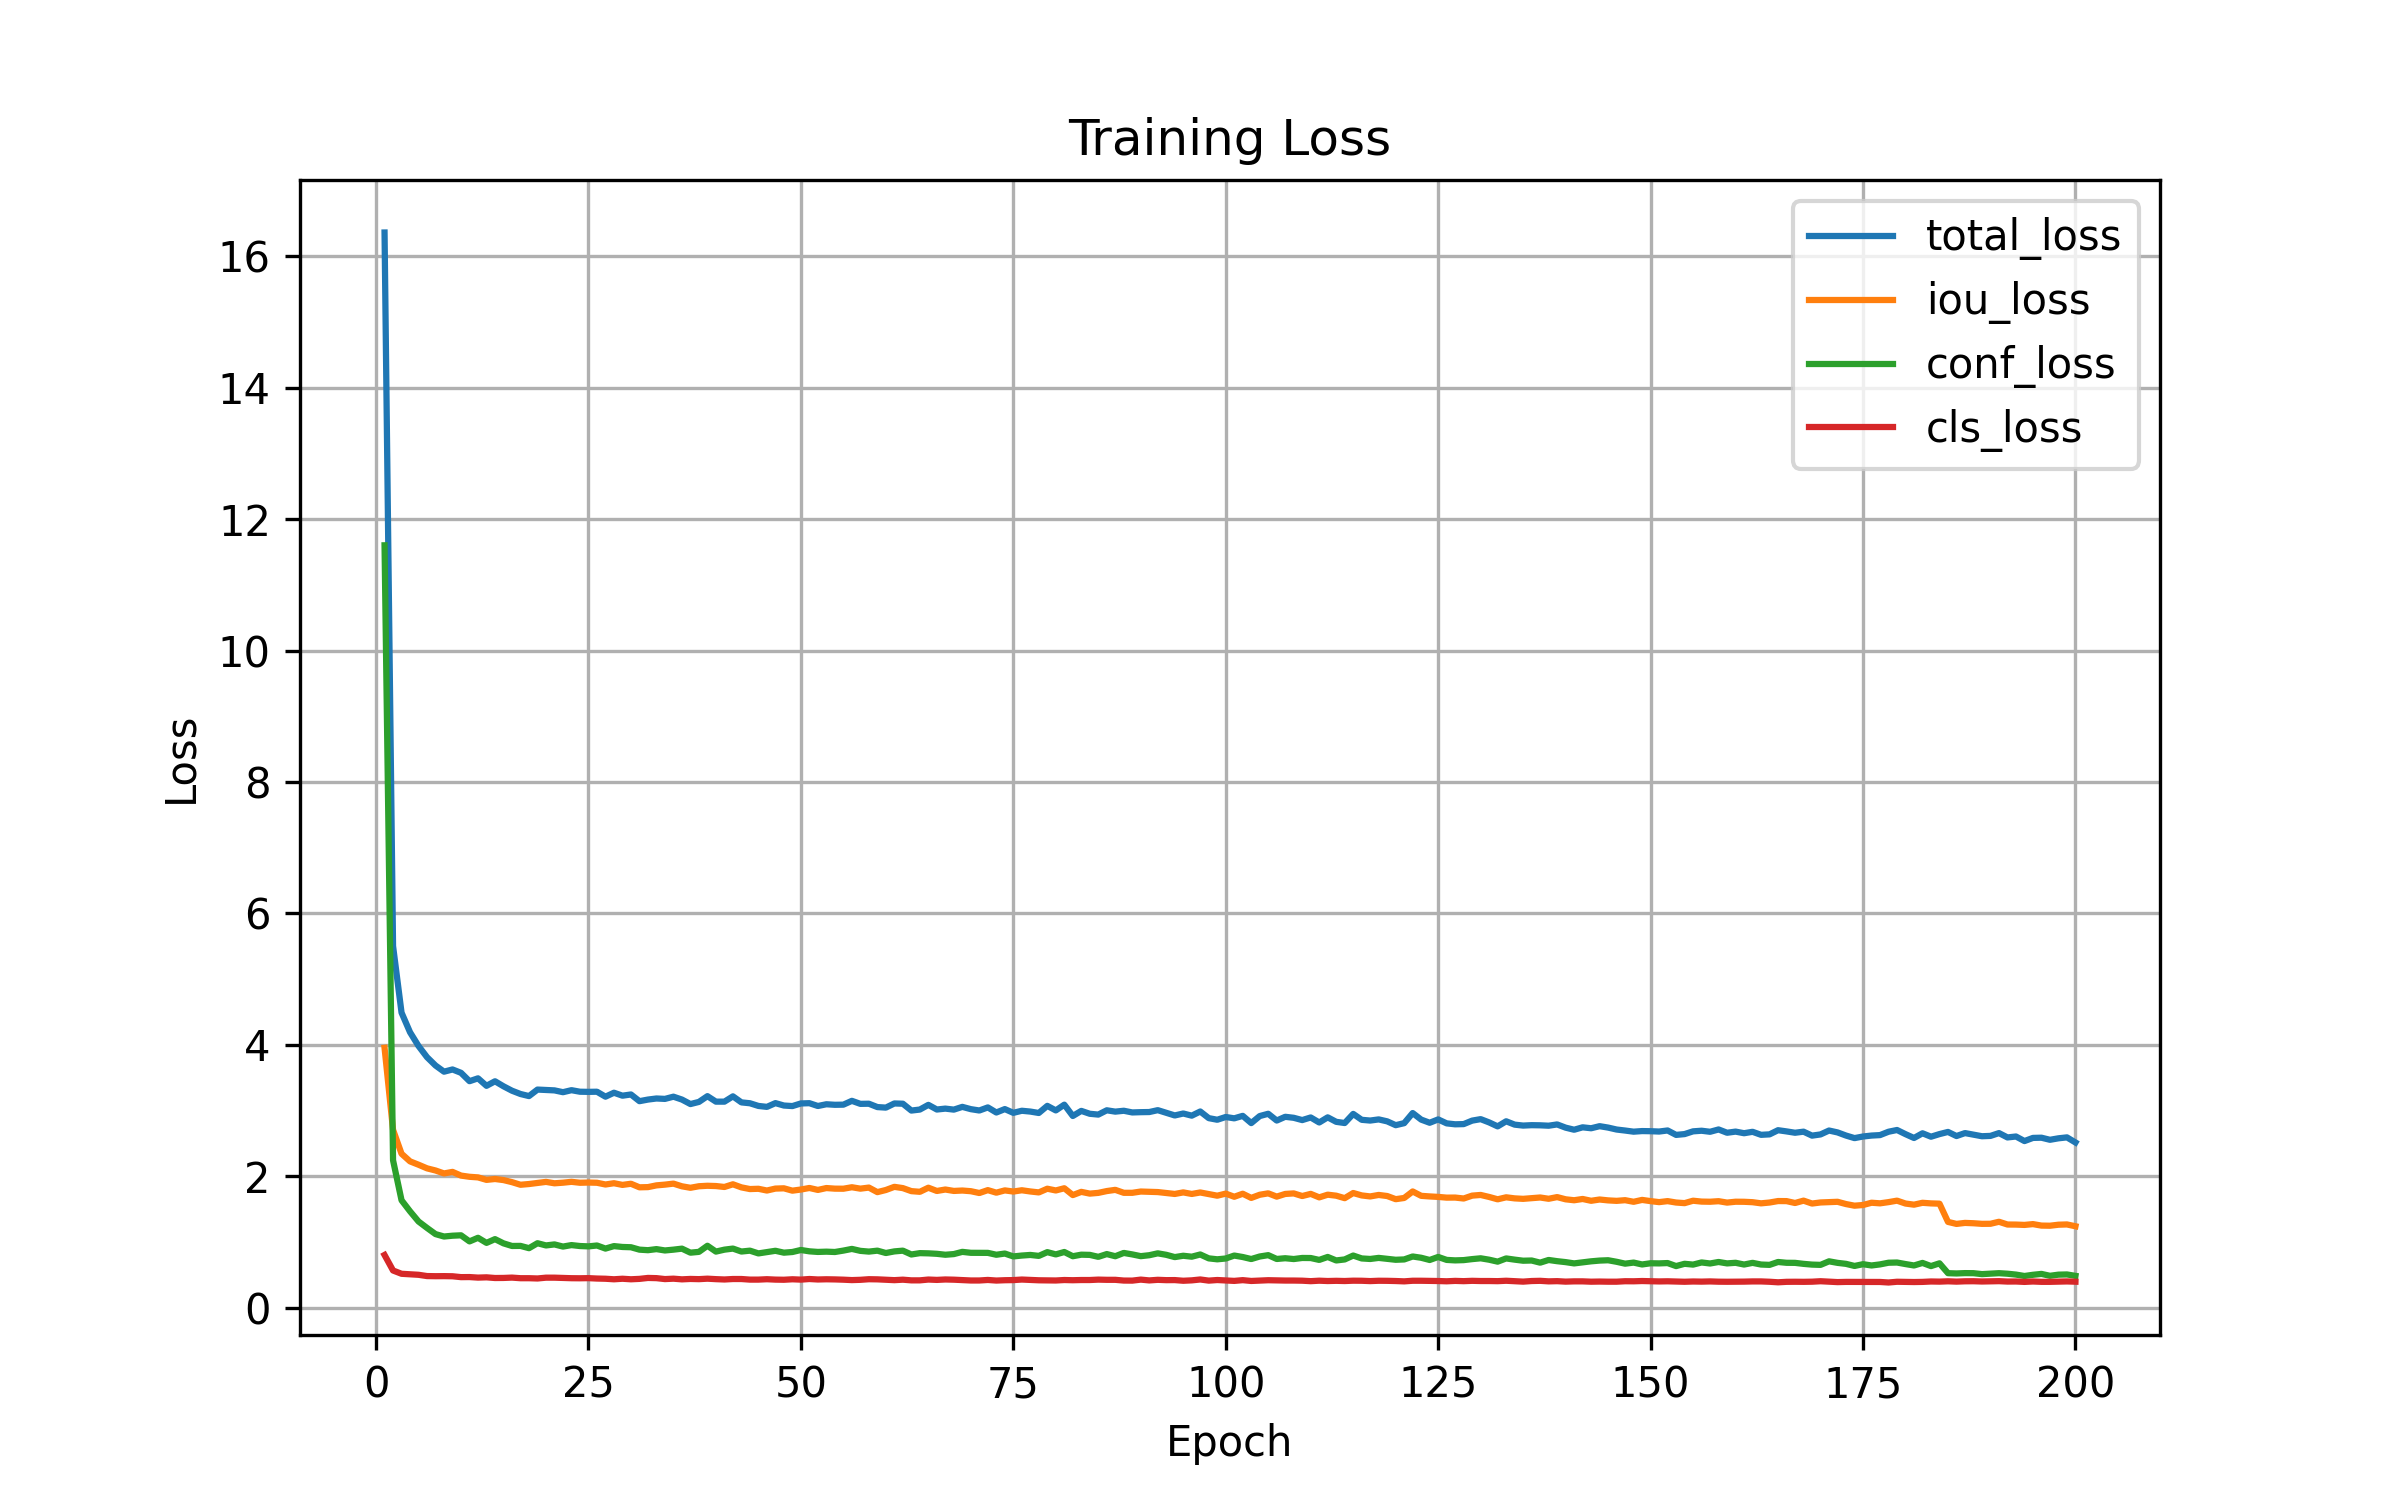
\includegraphics[width=\linewidth]{figures/images/chapter-11/licenseplate/v0/loss_curve.png}
\caption{Training loss}
\end{subfigure}
\hfill
\begin{subfigure}{0.48\textwidth}
\centering
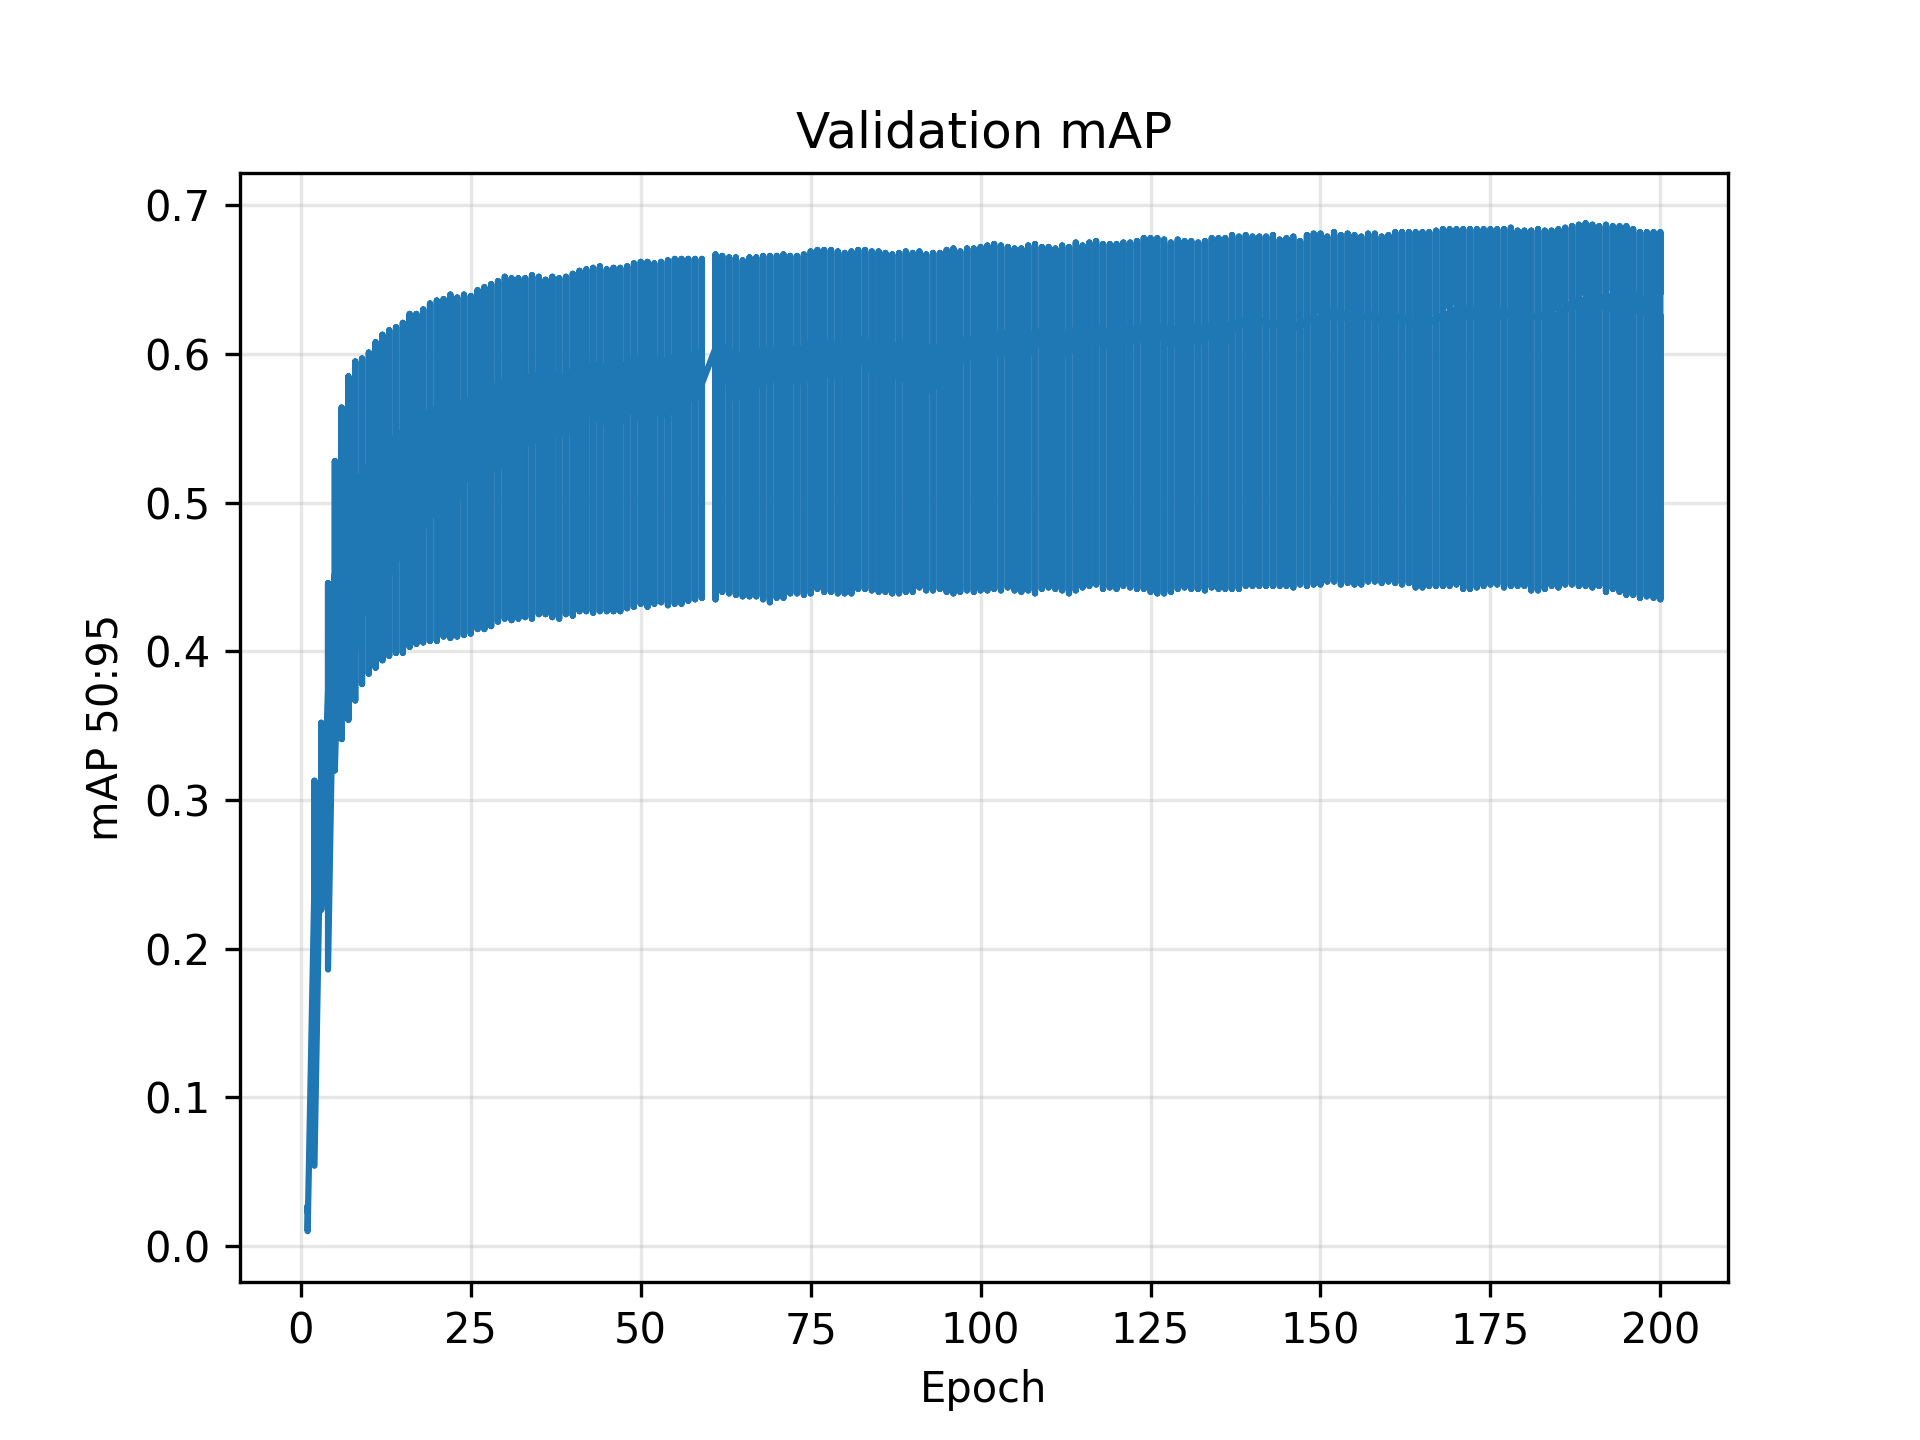
\includegraphics[width=\linewidth]{figures/images/chapter-11/licenseplate/v0/map_curve.png}
\caption{Validation mAP}
\end{subfigure}

\vspace{0.4cm}

\begin{subfigure}{0.50\textwidth}
\centering
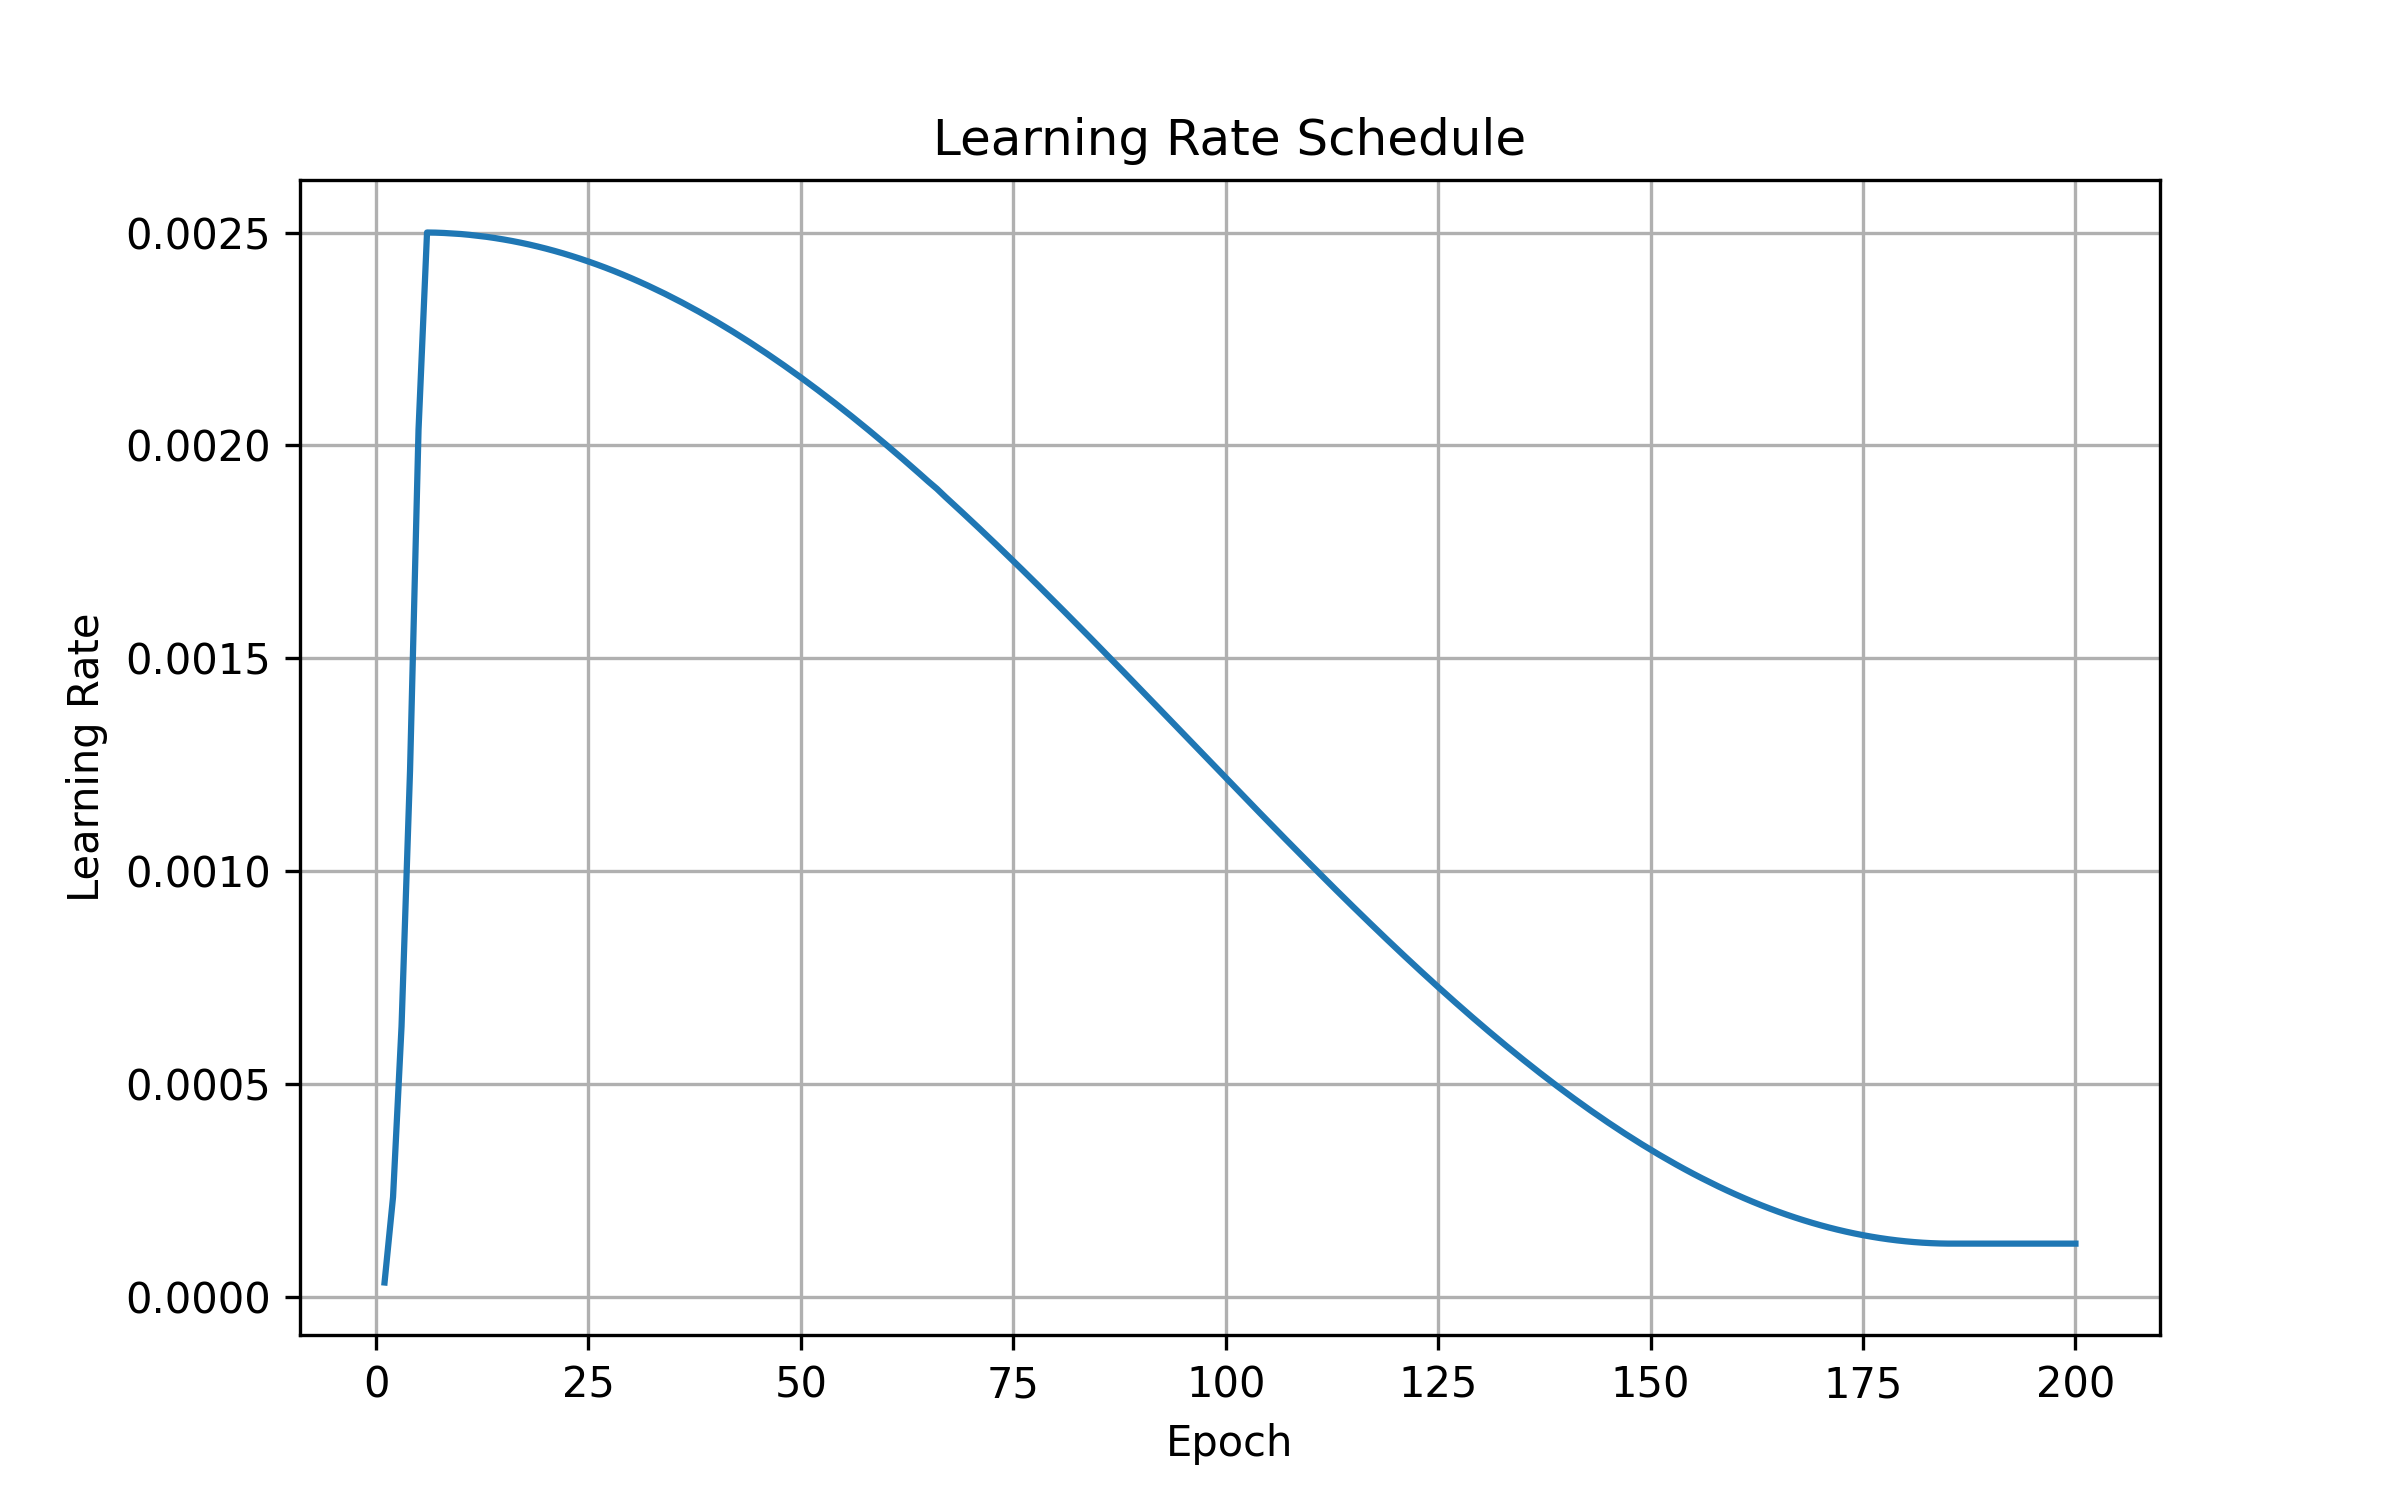
\includegraphics[width=\linewidth]{figures/images/chapter-11/licenseplate/v0/lr_curve.png}
\caption{Learning rate schedule}
\end{subfigure}

\caption{Training behaviour of model v0.}
\label{fig:lp_training_v0}

\end{figure}

\begin{figure}[H]
\centering

\begin{subfigure}{0.50\textwidth}
\centering
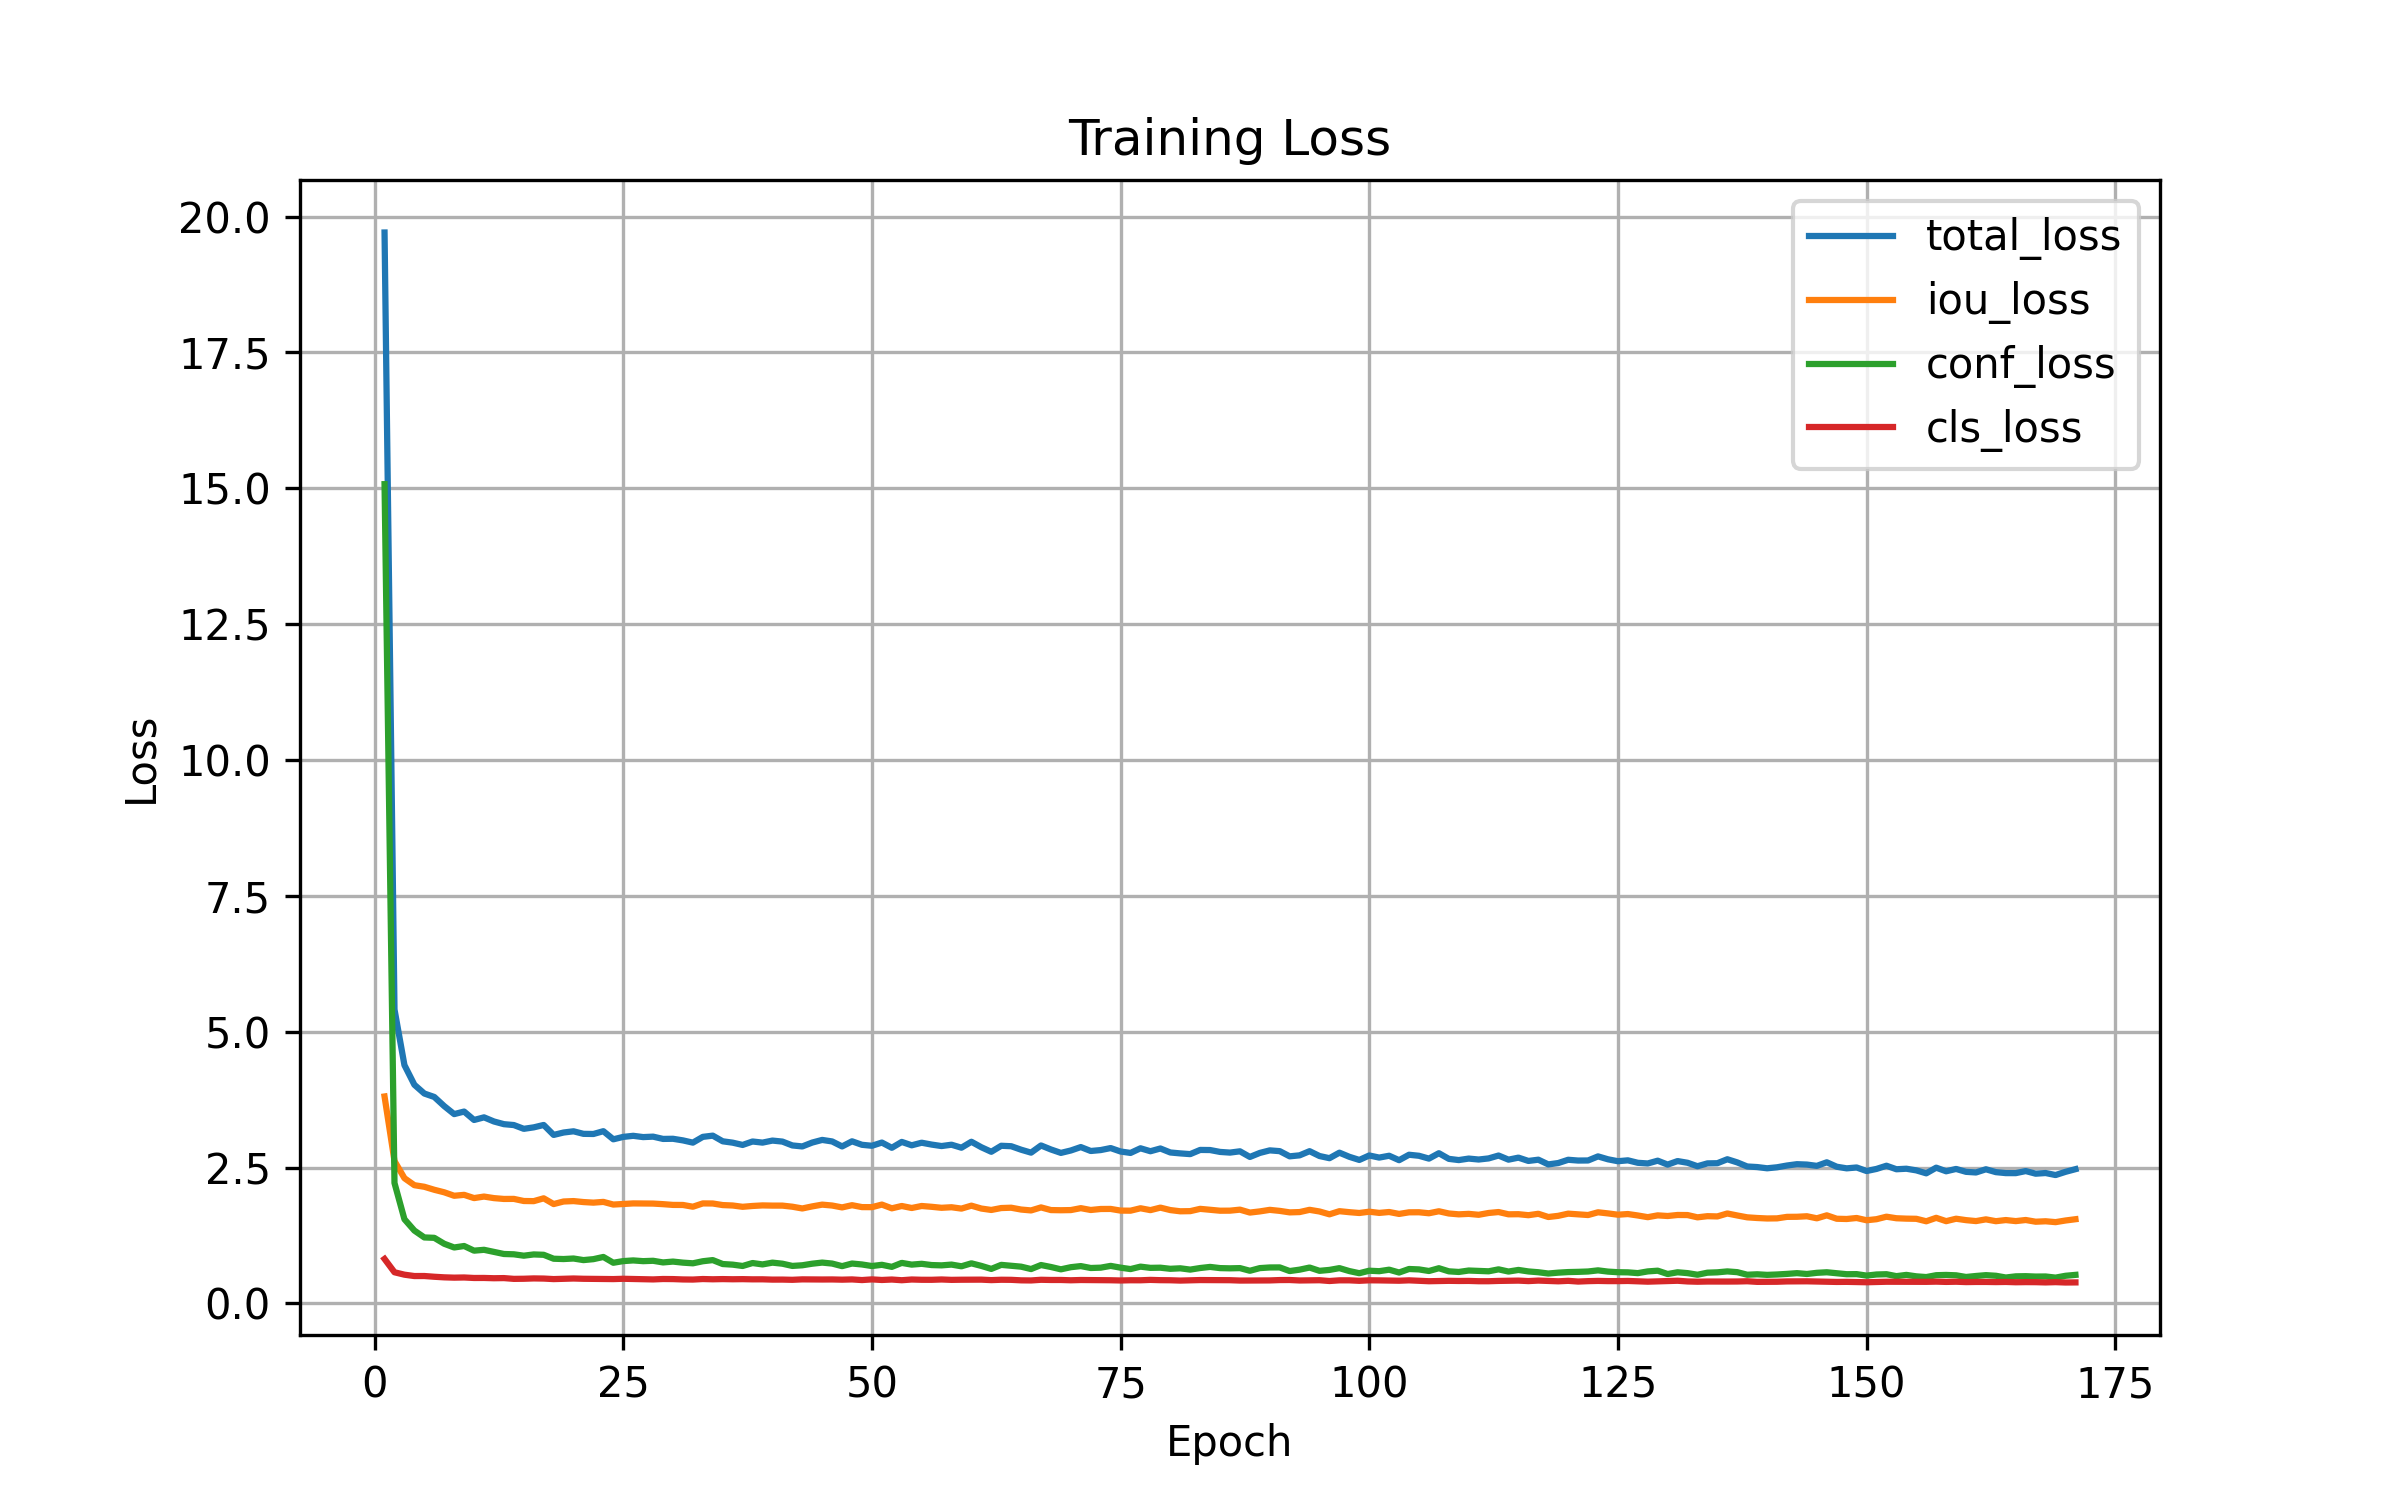
\includegraphics[width=\linewidth]{figures/images/chapter-11/licenseplate/v1/loss_curve.png}
\caption{Training loss}
\end{subfigure}
\hfill
\begin{subfigure}{0.48\textwidth}
\centering
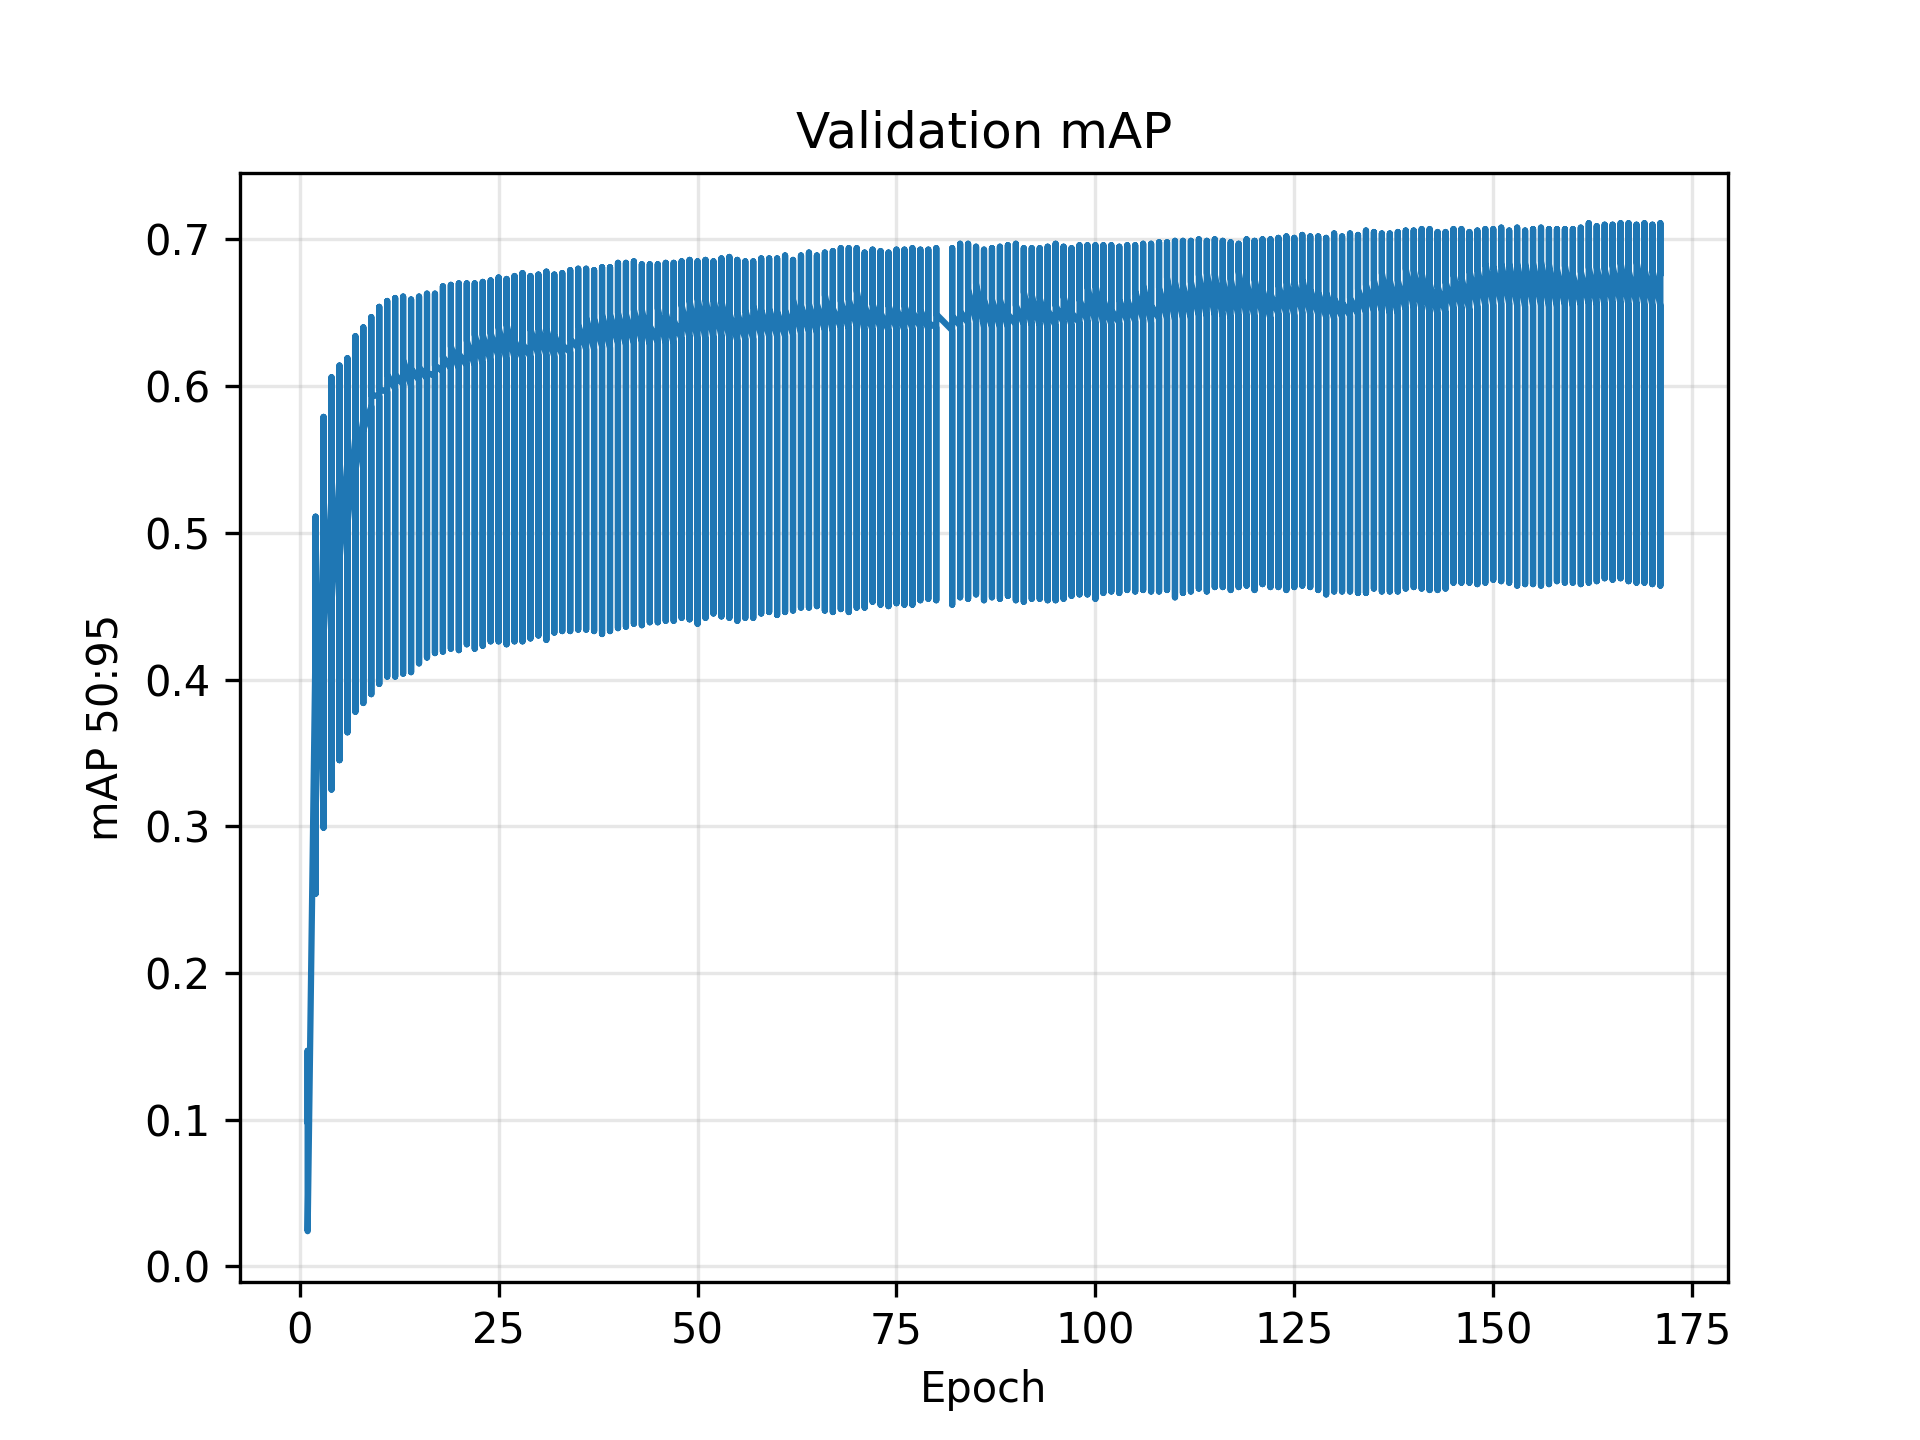
\includegraphics[width=\linewidth]{figures/images/chapter-11/licenseplate/v1/map_curve.png}
\caption{Validation mAP}
\end{subfigure}

\vspace{0.4cm}

\begin{subfigure}{0.50\textwidth}
\centering
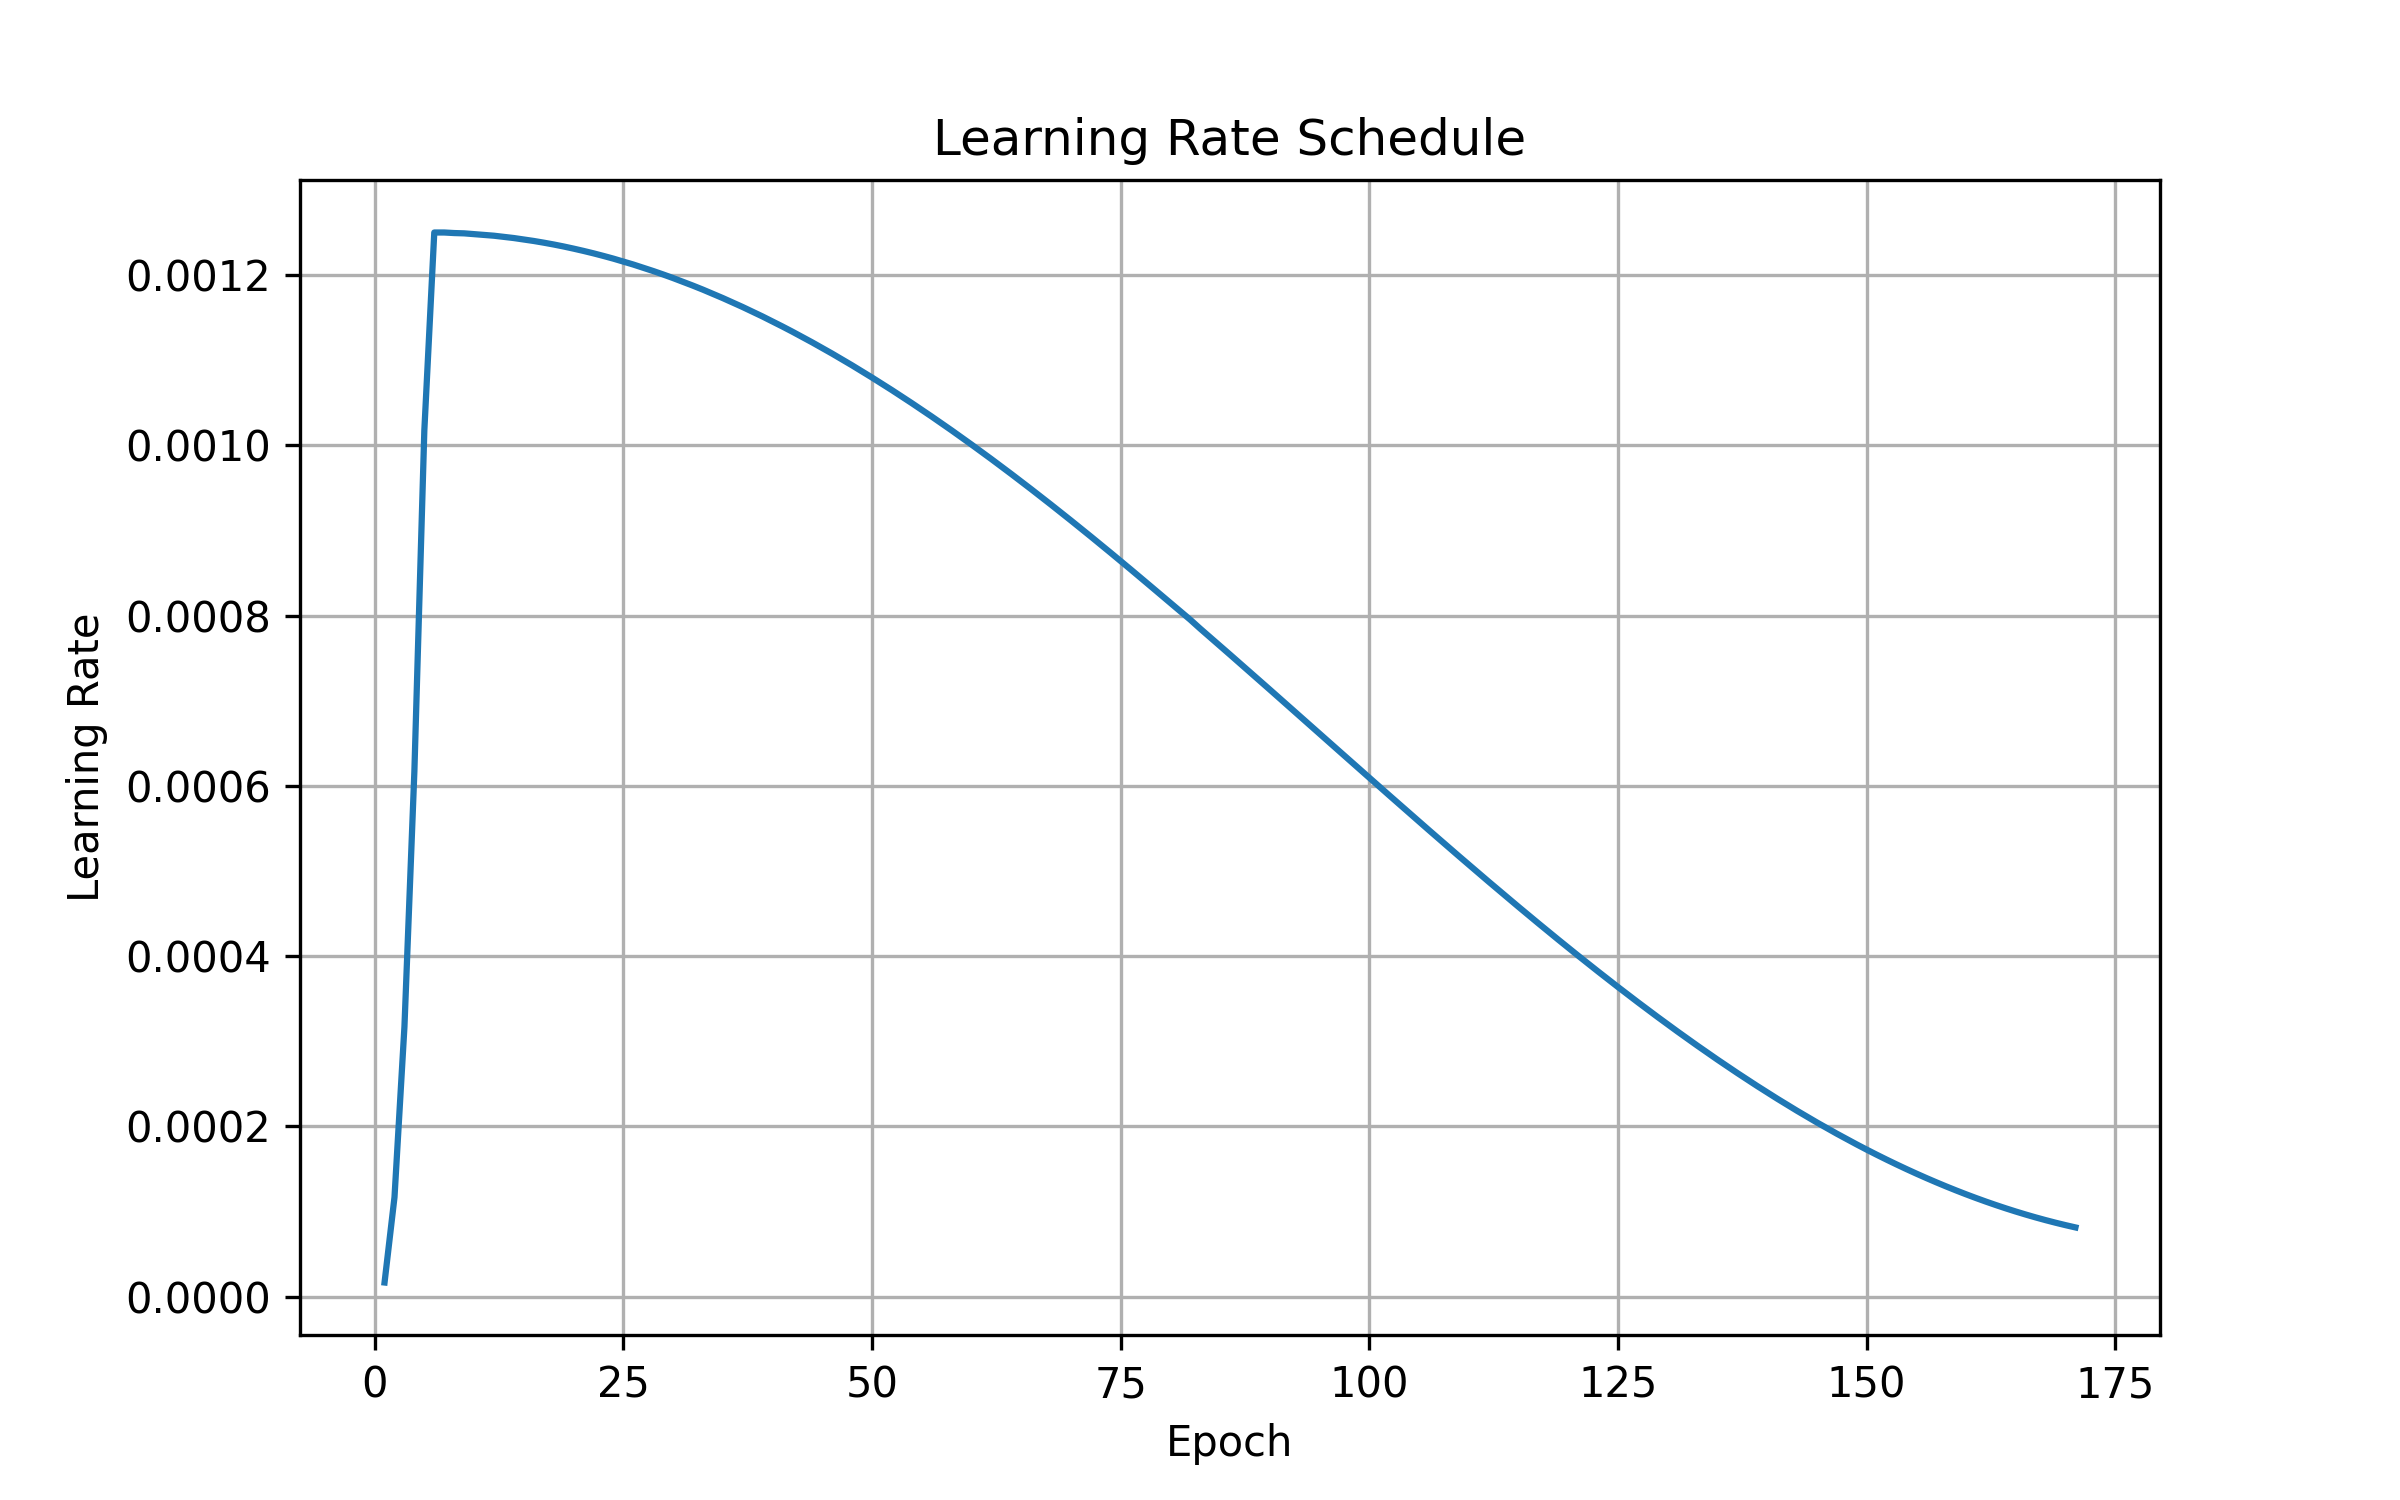
\includegraphics[width=\linewidth]{figures/images/chapter-11/licenseplate/v1/lr_curve.png}
\caption{Learning rate schedule}
\end{subfigure}

\caption{Training behaviour of model v1.}
\label{fig:lp_training_v1}

\end{figure}

Figure~\ref{fig:lp_training_v0} and Figure~\ref{fig:lp_training_v1} show the
training behaviour of the two license plate detection models. For both models,
the training loss decreases rapidly during the first epochs and then gradually
stabilizes, indicating stable optimization.

The validation mAP increases quickly at the beginning of training and then
continues to improve more gradually. Model v0 was trained for the full 200
epochs, while model v1 stopped earlier at approximately 175 epochs due to the
early stopping criterion. In both cases, the learning rate follows the expected
warm-up and decay schedule.







\subsection{Precision--Recall Analysis}

\begin{figure}[H]
\centering

\begin{subfigure}{0.48\textwidth}
\centering
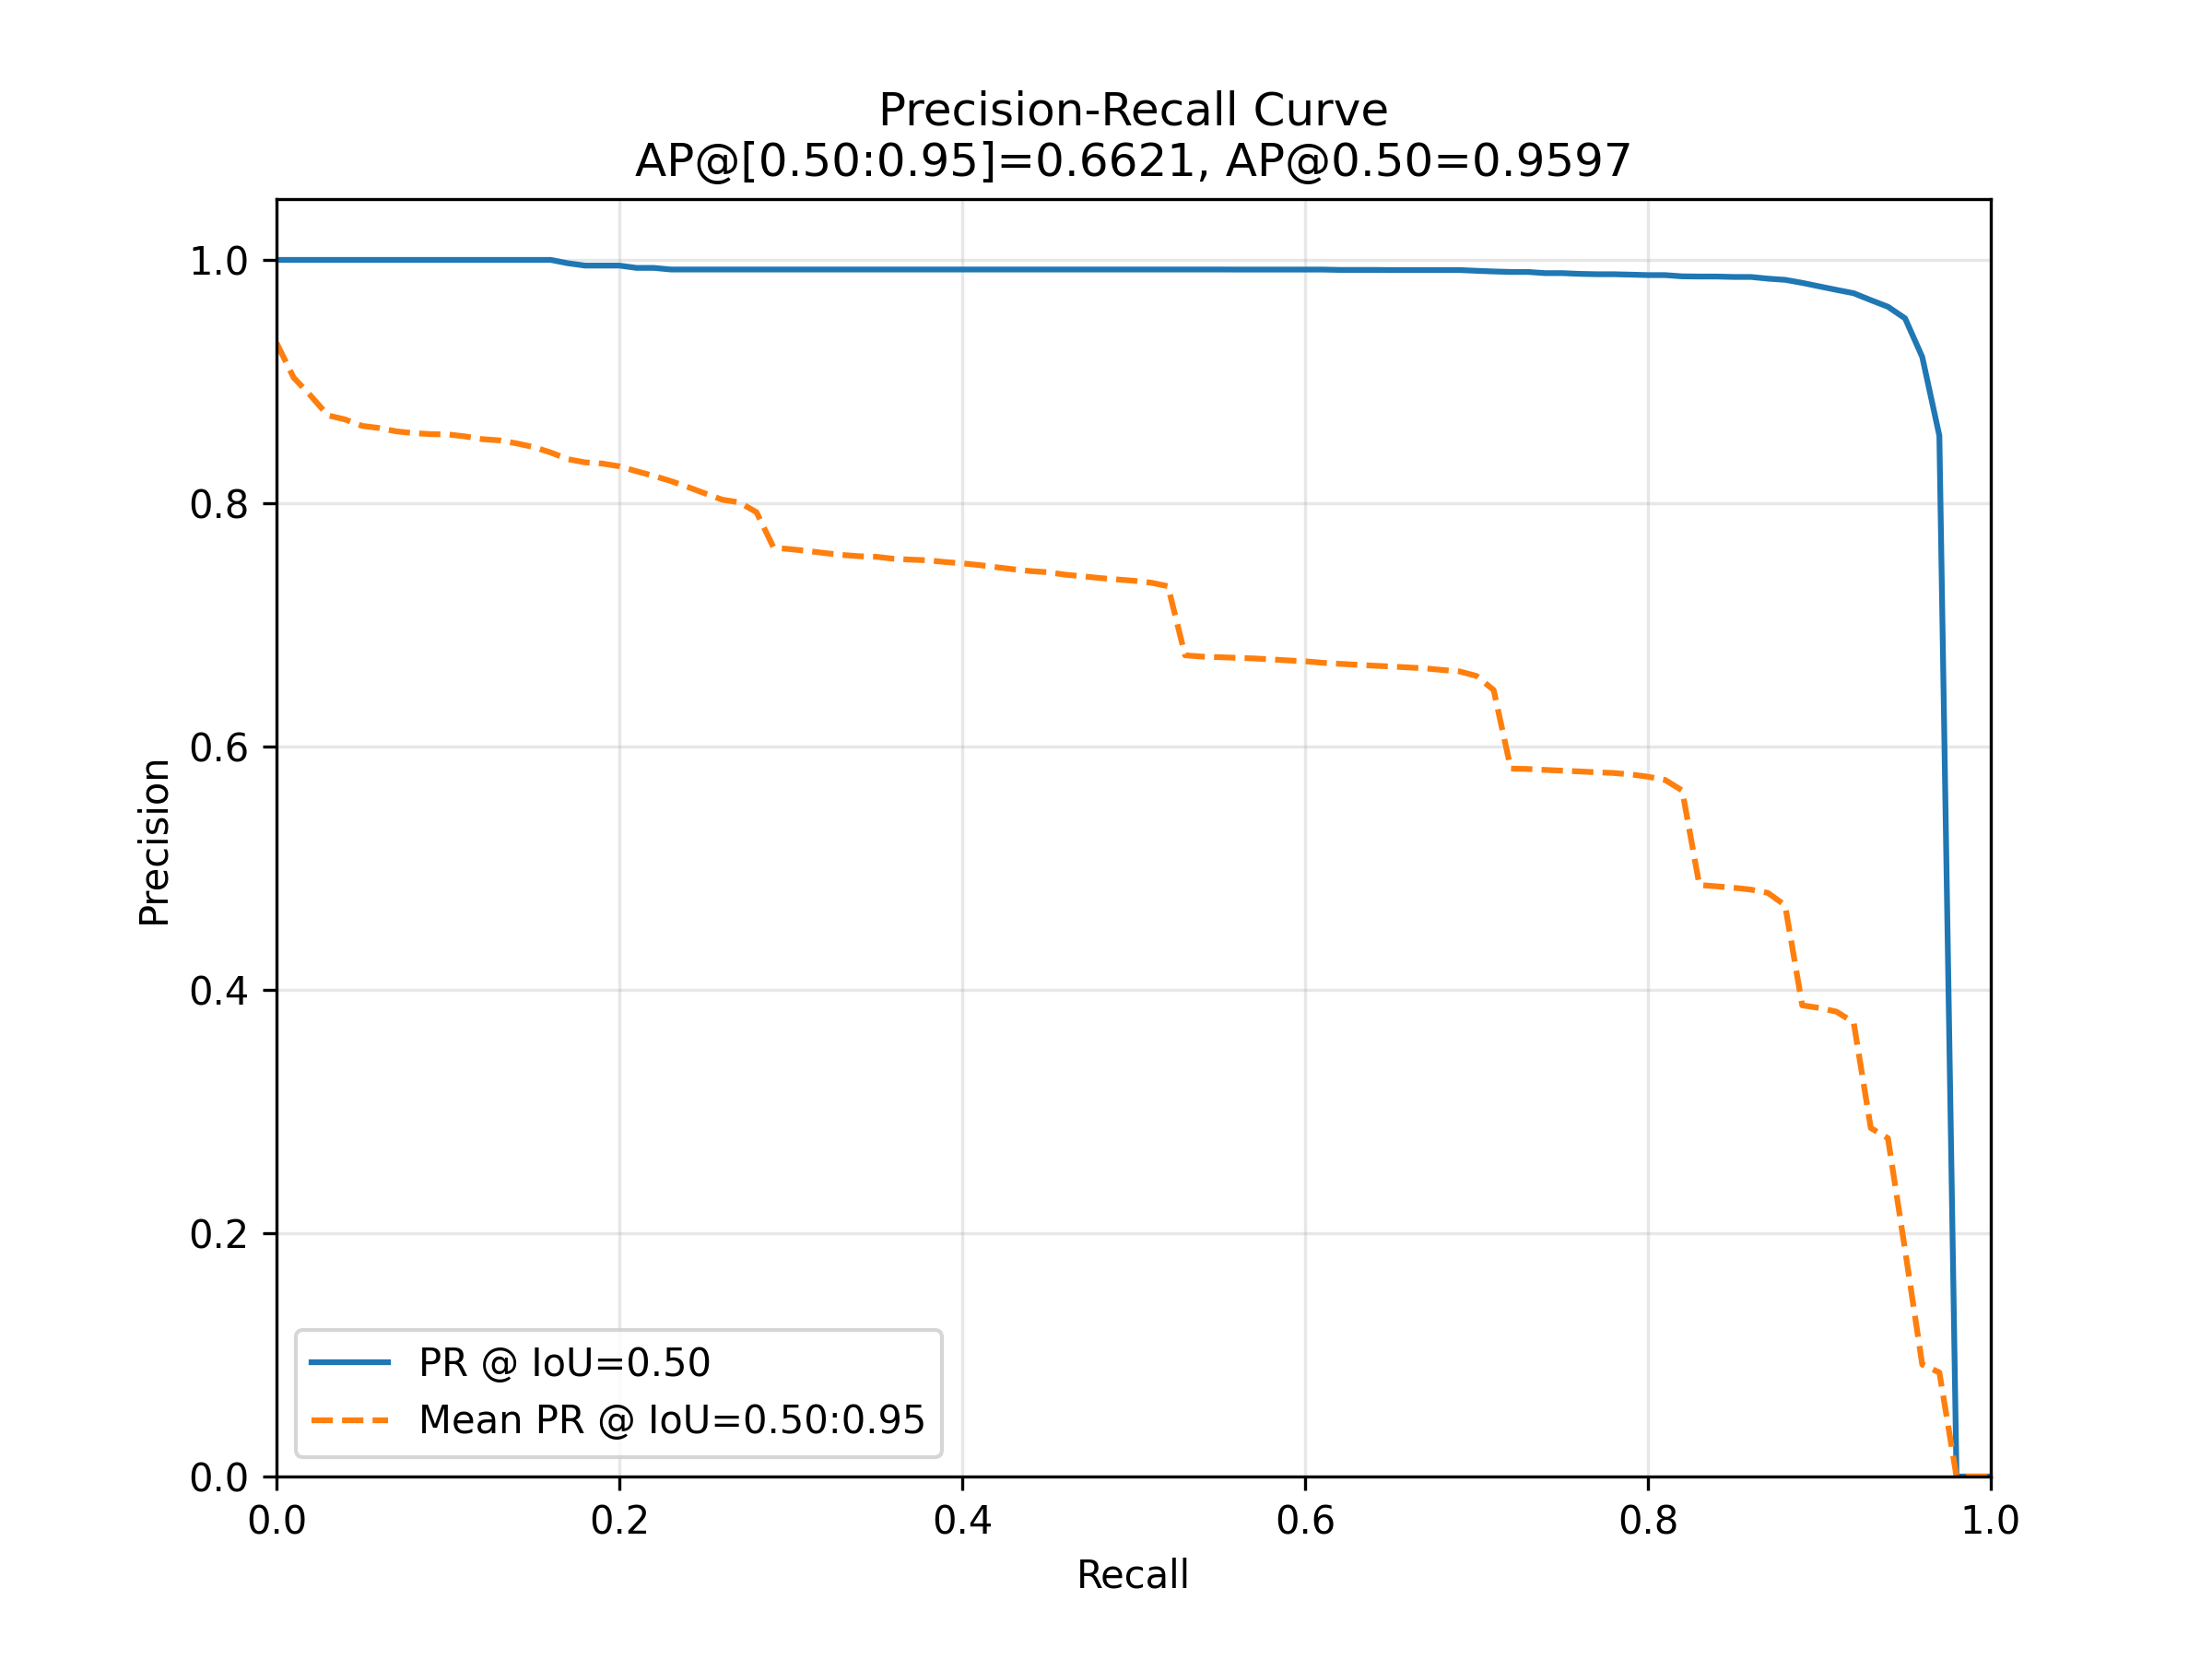
\includegraphics[width=\linewidth]{figures/images/chapter-11/licenseplate/v0/pr_curve.png}
\caption{V0 configuration.}
\end{subfigure}
\hfill
\begin{subfigure}{0.48\textwidth}
\centering
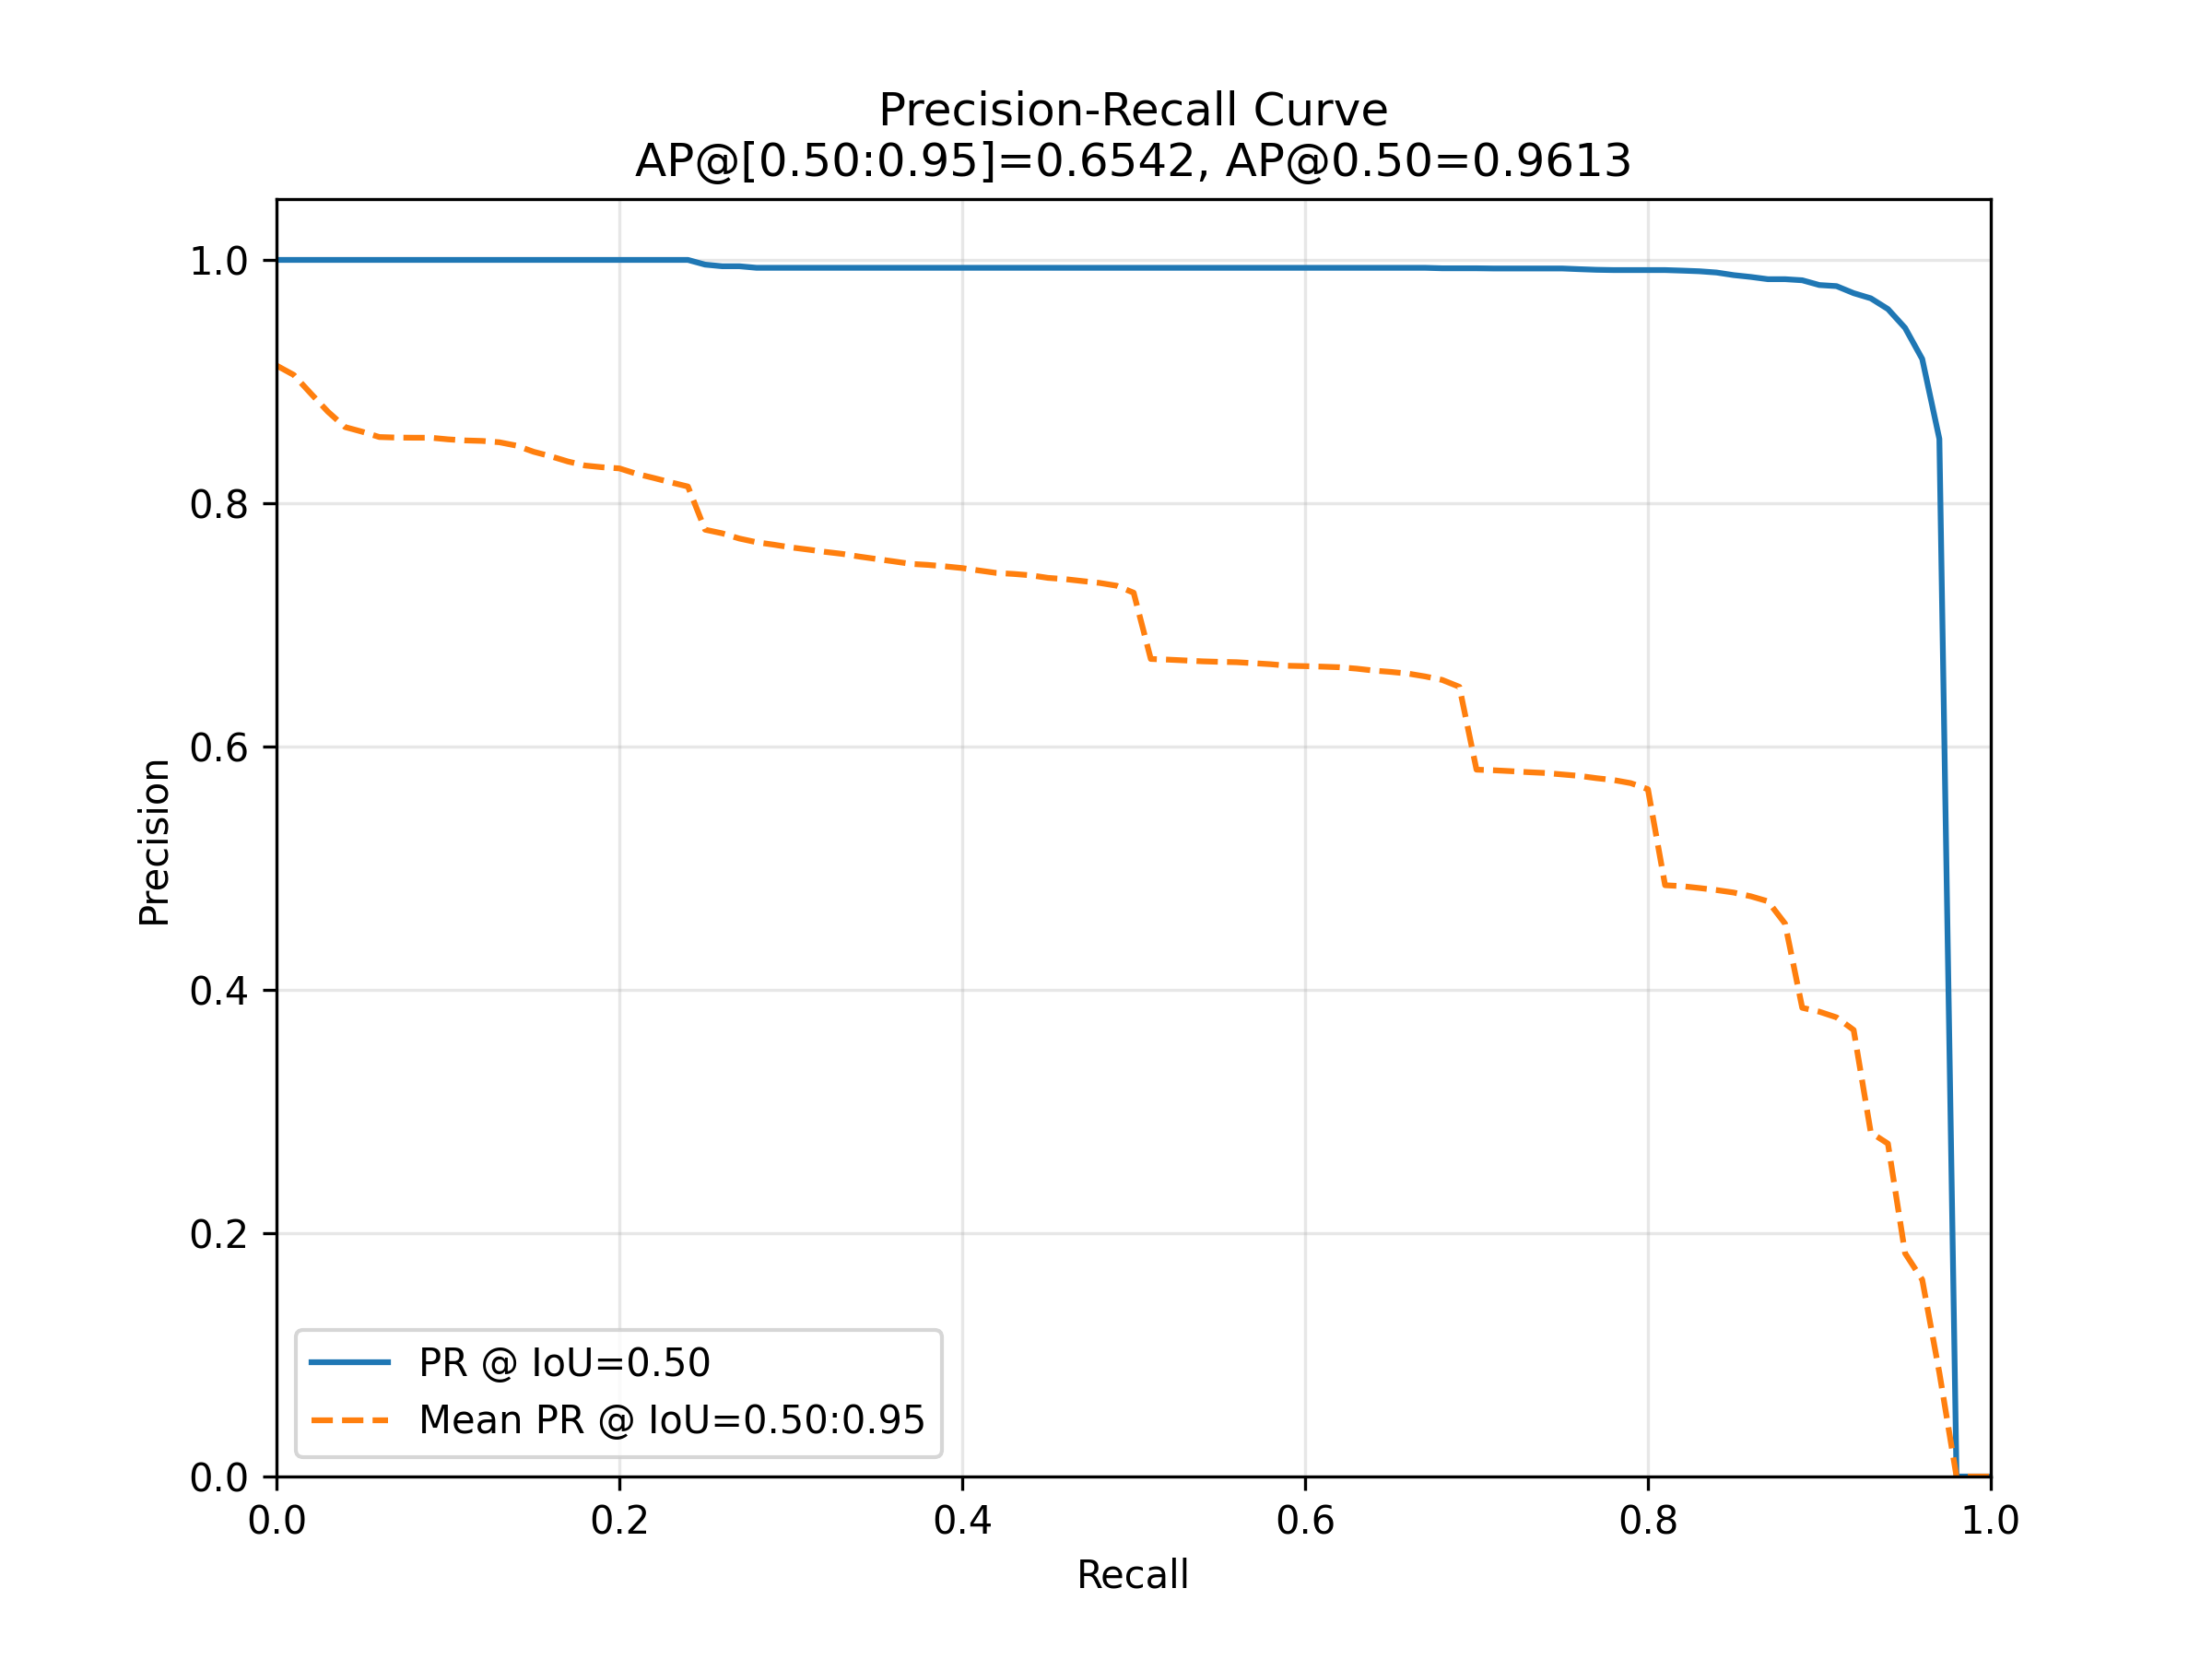
\includegraphics[width=\linewidth]{figures/images/chapter-11/licenseplate/v1/pr_curve.png}
\caption{V1 configuration.}
\end{subfigure}

\caption{Side-by-side comparison of the precision--recall curves for the v0 and v1 configurations.}
\label{fig:lp_pr_curves_licenseplate} 
\end{figure}

Figure~\ref{fig:lp_pr_curves_licenseplate} shows the precision--recall curves for the two
license plate detection models. Both configurations achieve a high AP@0.50,
with v0 reaching 0.9597 and v1 reaching 0.9613. This indicates strong detection
performance for both models at an IoU threshold of 0.50.

The AP@0.50:0.95 values are also similar, with v0 achieving 0.6621 and v1
achieving 0.6542. Although v1 performs slightly better at AP@0.50, v0 obtains a
slightly higher score across the stricter IoU range. Overall, the
precision--recall analysis shows that the two configurations perform similarly,
with only small differences between them.





\subsection{Confusion Matrix Analysis}

\begin{figure}[H]
\centering
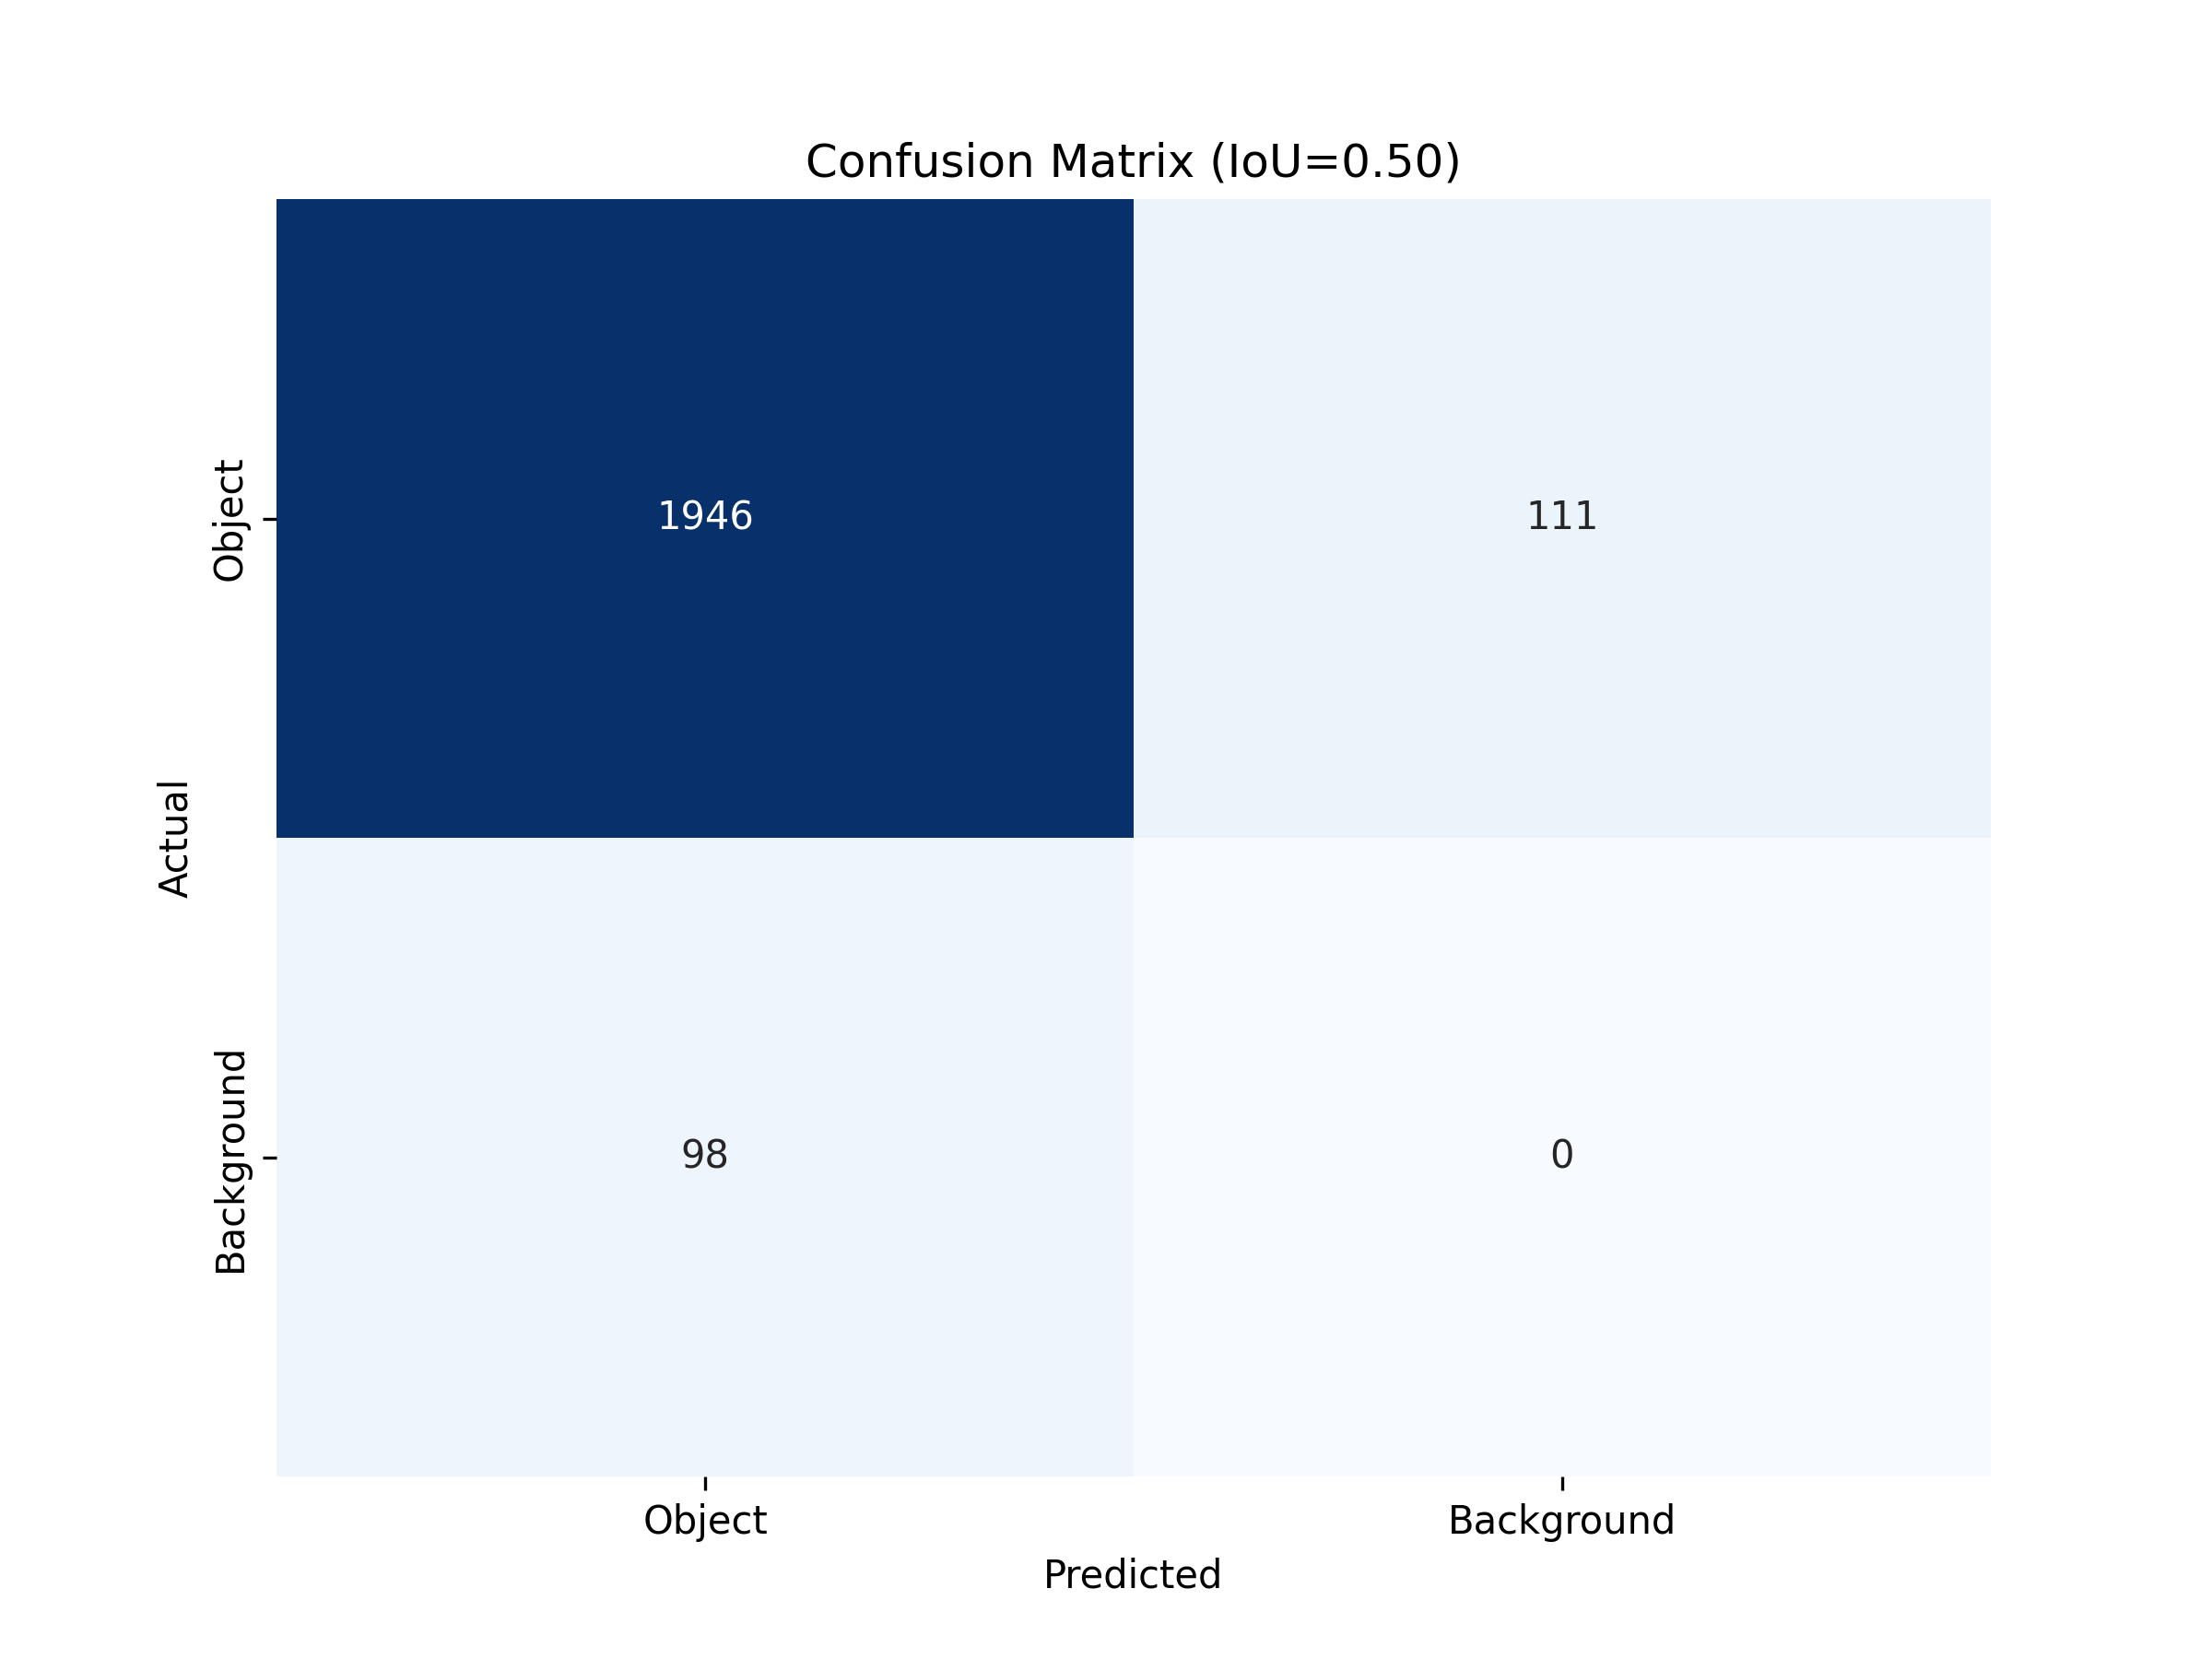
\includegraphics[width=12cm]{figures/images/chapter-11/licenseplate/v0/confusion_matrix_0.3.png}
\caption{Confusion matrix for the v0 configuration.}
\label{fig:lp_confusion_matrix_v0}
\end{figure}

\begin{figure}[H]
\centering
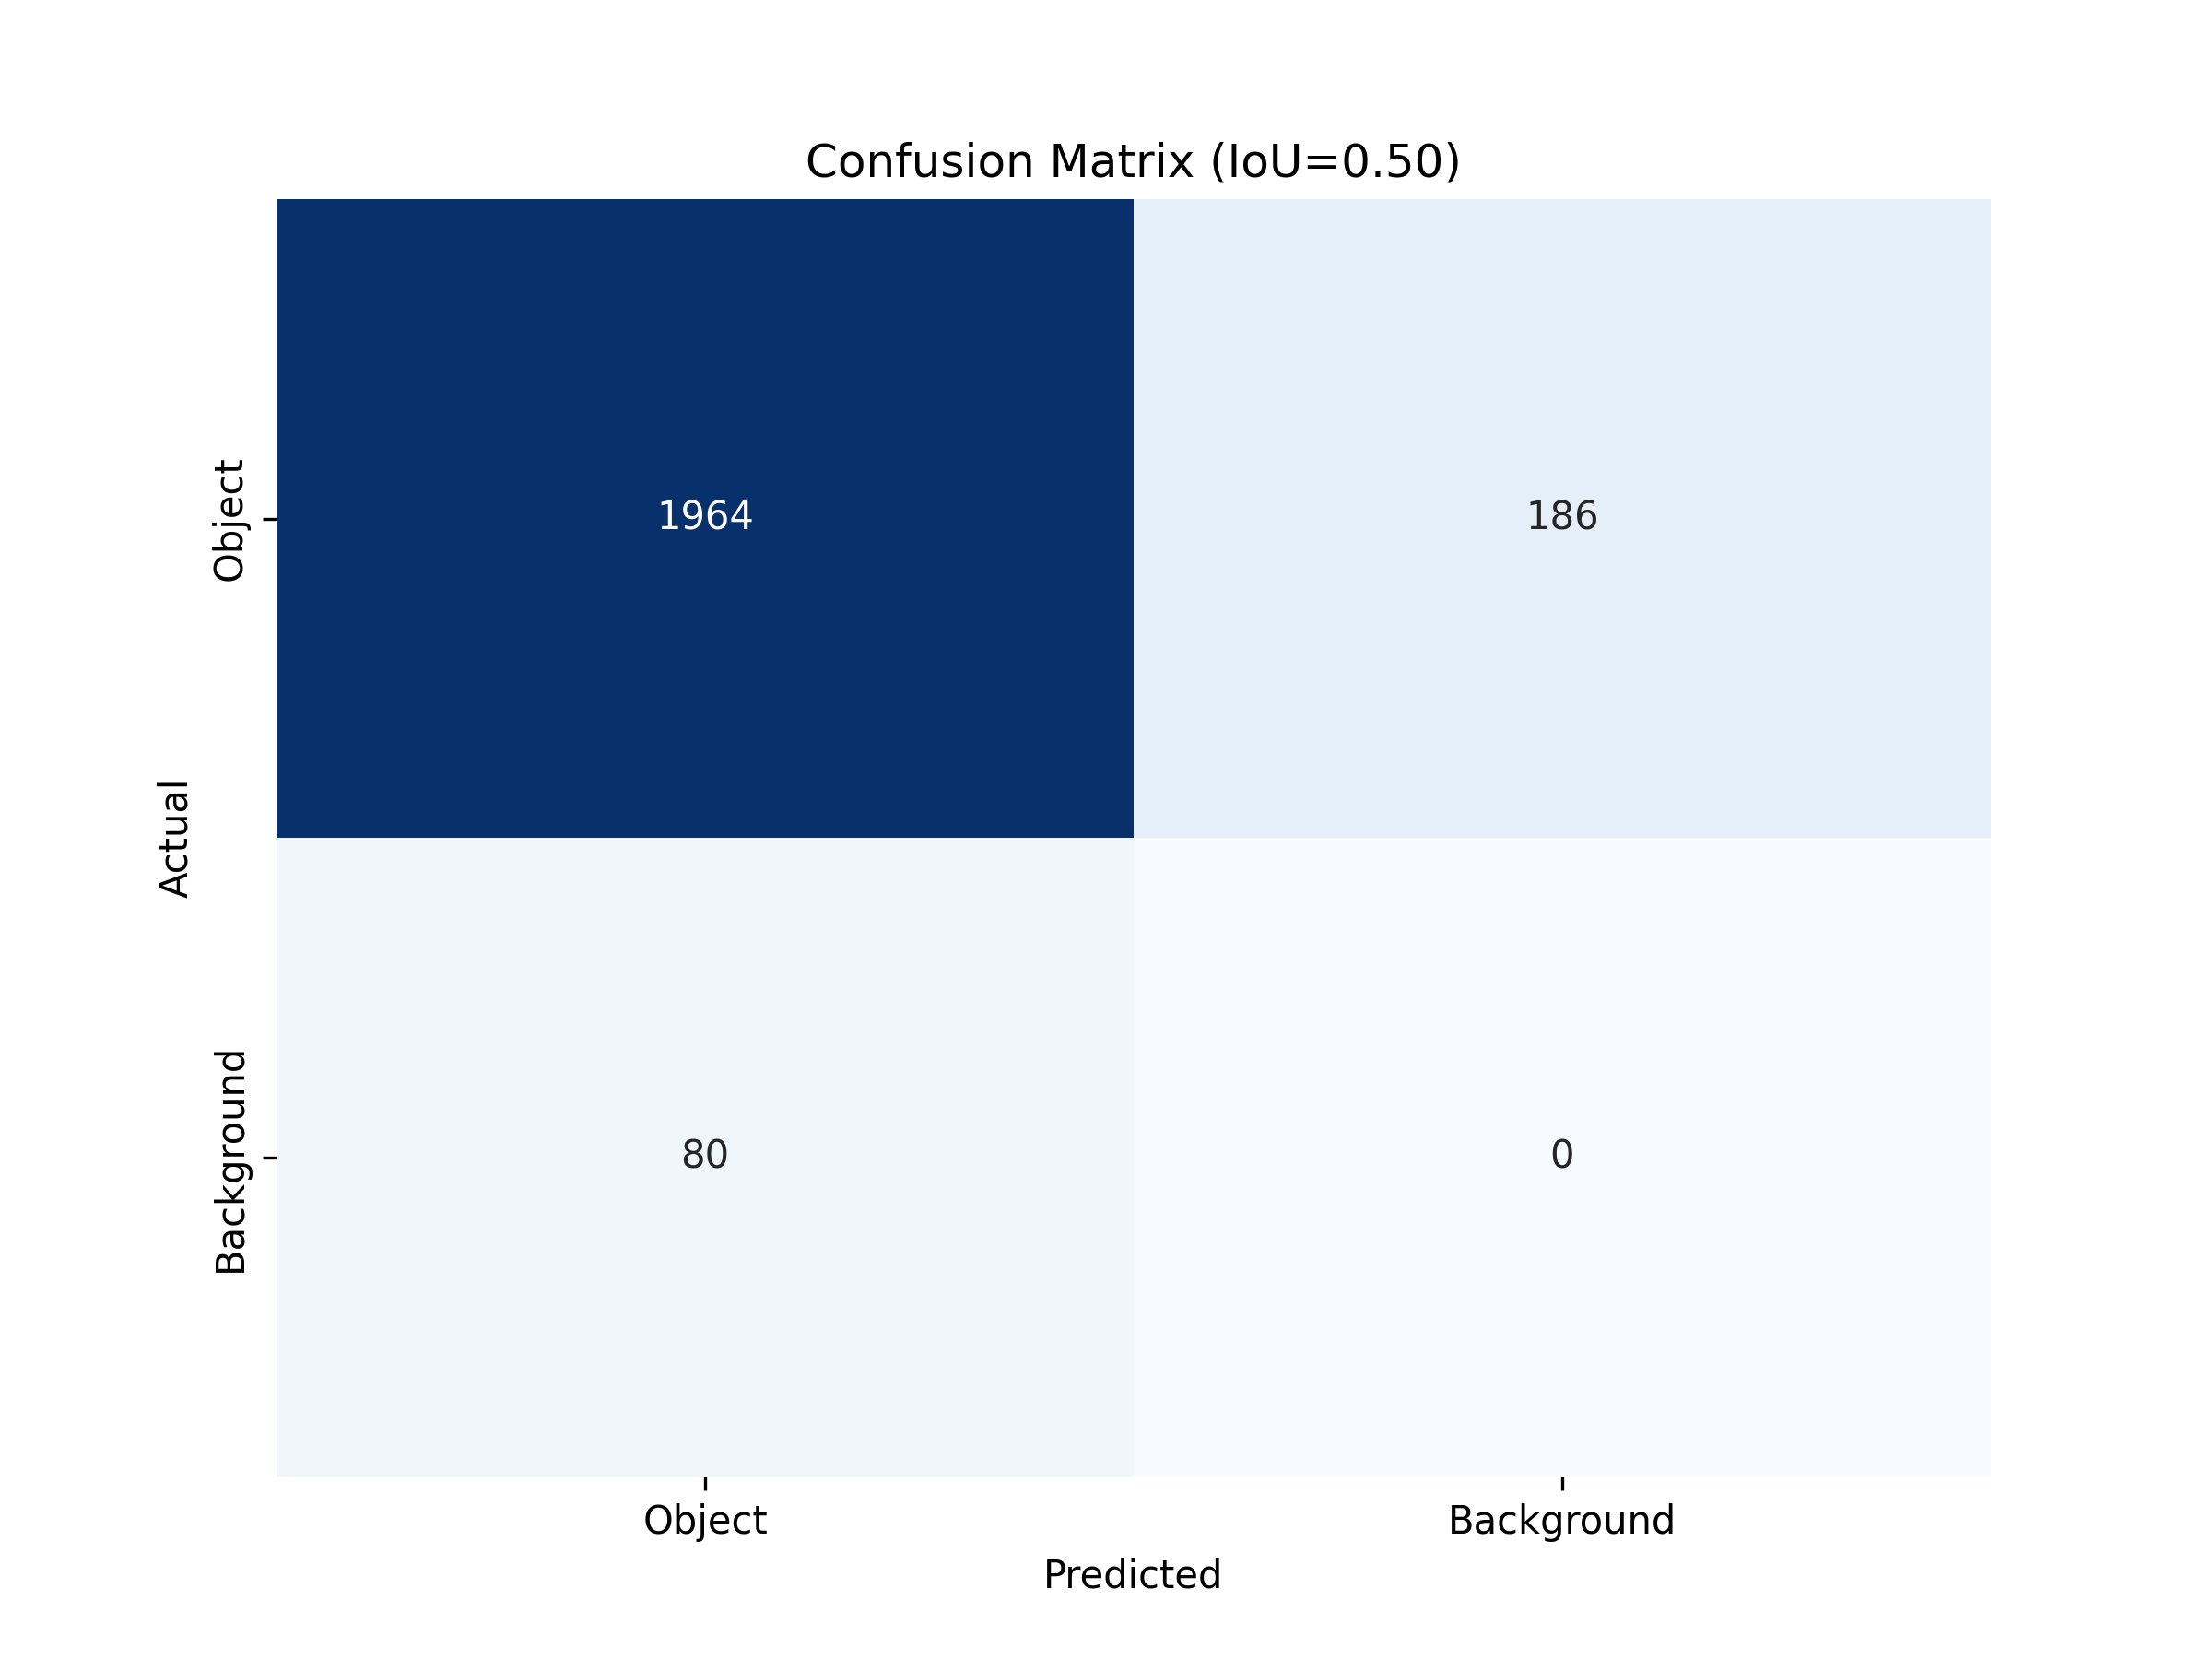
\includegraphics[width=12cm]{figures/images/chapter-11/licenseplate/v1/confusion_matrix_0.3.png}
\caption{Confusion matrix for the v1 configuration.}
\label{fig:lp_confusion_matrix_v1}
\end{figure}

Figure~\ref{fig:lp_confusion_matrix_v0} and
Figure~\ref{fig:lp_confusion_matrix_v1} show the confusion matrices for the two
license plate detection models at an IoU threshold of 0.50.

The confusion matrix values do not directly match the number of test images
because object detection is evaluated at the object level. Each image may
contain multiple license plates and multiple predicted bounding boxes.
Therefore, the matrix counts detections and missed objects rather than images.

The F1-score was calculated as the harmonic mean of precision and recall:
\[
F1 = 2 \cdot \frac{Precision \cdot Recall}{Precision + Recall}
\]

The v0 configuration correctly detected 1946 license plates, produced 98 false
positive detections, and missed 111 license plates. This resulted in a
precision of 0.9521, a recall of 0.9460, and an F1-score of 0.9490.

The v1 configuration correctly detected 1964 license plates and produced fewer
false positives, with 80 false detections. However, it also missed more license
plates, with 186 false negatives. This resulted in a slightly higher precision
of 0.9609, but a lower recall of 0.9135 and an F1-score of 0.9366.

\begin{align*}
Precision_{v0} &= \frac{1946}{1946 + 98} \approx 0.9521,
&
Recall_{v0} &= \frac{1946}{1946 + 111} \approx 0.9460,
&
F1_{v0} &\approx 0.9490
\end{align*}

\begin{align*}
Precision_{v1} &= \frac{1964}{1964 + 80} \approx 0.9609,
&
Recall_{v1} &= \frac{1964}{1964 + 186} \approx 0.9135,
&
F1_{v1} &\approx 0.9366
\end{align*}

Overall, v1 is slightly more precise, while v0 achieves better recall and a
higher F1-score. This indicates that v0 provides a better balance between
detecting license plates and avoiding false detections.

\subsection{Summary}

Both license plate detection models achieved strong detection performance on
the unseen test set. Model v1 obtained slightly higher precision, while model
v0 achieved higher recall and a higher F1-score.

Since the proposed system benefits from detecting as many license plates as
possible while still maintaining high precision, the v0 configuration was
selected as the final license plate detection model. The results show that v0
provides the best overall balance between precision, recall, and F1-score. The final barcode detection model was therefore selected for use in the proposed system.










% --------------------------------------------------------------------------------


\section{Named Entity Recognition}
\label{app:ner_evaluation}

\subsection{Training Setup}

The NER model was trained as a token classification model based on XLM-RoBERTa. Unlike the barcode and license plate models, which were trained as object detectors, the NER component addressed sequence labeling of \acrshort{ocr} extracted text. The training workflow combined synthetically generated data with converted external NER datasets in order to balance \acrshort{ocr} specific privacy entities with more natural running-text examples.

\begin{table}[H]
\centering
\begin{tabular}{l r}
\toprule
\textbf{Dataset source} & \textbf{Samples} \\
\midrule
Synthetic dataset & 199000 \\
NorNE (converted) \cite{norne_sprakbanken} & 15000 \\
English NER dataset (converted) \cite{kaggle_ner_dataset} & 15000 \\
\midrule
Total merged dataset & 229000 \\
\bottomrule
\end{tabular}
\caption{Composition of the merged NER dataset used before train/validation/test splitting.}
\label{tab:ner_dataset_composition}
\end{table}

\begin{table}[H]
\centering
\begin{tabular}{l r}
\toprule
\textbf{Split} & \textbf{Samples} \\
\midrule
Train & 183200 \\
Validation & 22900 \\
Test & 22900 \\
\bottomrule
\end{tabular}
\caption{Final split sizes for the merged NER dataset.}
\label{tab:ner_final_splits}
\end{table}

As shown in Tables~\ref{tab:ner_dataset_composition} and~\ref{tab:ner_final_splits},
the training data consisted primarily of synthetic samples, while smaller converted
Norwegian and English NER datasets were included to strengthen the recognition of
more general entity types in running text.

\subsection{Training Configuration}

The model was trained using the Hugging Face Transformers framework with
\texttt{FacebookAI/xlm-roberta-base} as the pretrained backbone. Training was
performed as a BIO-formatted token classification task.

\begin{table}[H]
\centering
\begin{tabular}{l l}
\toprule
\textbf{Parameter} & \textbf{Value} \\
\midrule
Backbone & XLM-RoBERTa base \\
Task type & Token classification \\
Max sequence length & 256 \\
Epochs & 6 \\
Learning rate & \(3 \times 10^{-5}\) \\
Train batch size & 8 \\
Evaluation batch size & 16 \\
Evaluation strategy & Per epoch \\
Save strategy & Per epoch \\
Mixed precision & Enabled when CUDA was available \\
\bottomrule
\end{tabular}
\caption{Final training configuration for the NER model.}
\label{tab:ner_training_config}
\end{table}

The selected configuration was intended to provide a lightweight fine-tuning setup
while remaining feasible within the available hardware constraints.

\subsection{Training Curves}

Figures~\ref{fig:ner_train_loss} and~\ref{fig:ner_validation_metrics} summarize the
training process. The training loss decreased sharply during the early training steps
and then gradually stabilized at a very low level. The validation loss also decreased
overall across epochs, although a temporary increase was observed around epoch 4.
Similarly, the validation F1 improved overall during training, despite a short-lived
drop at epoch 4, and reached its highest value in the final epoch.

\begin{figure}[H]
\centering
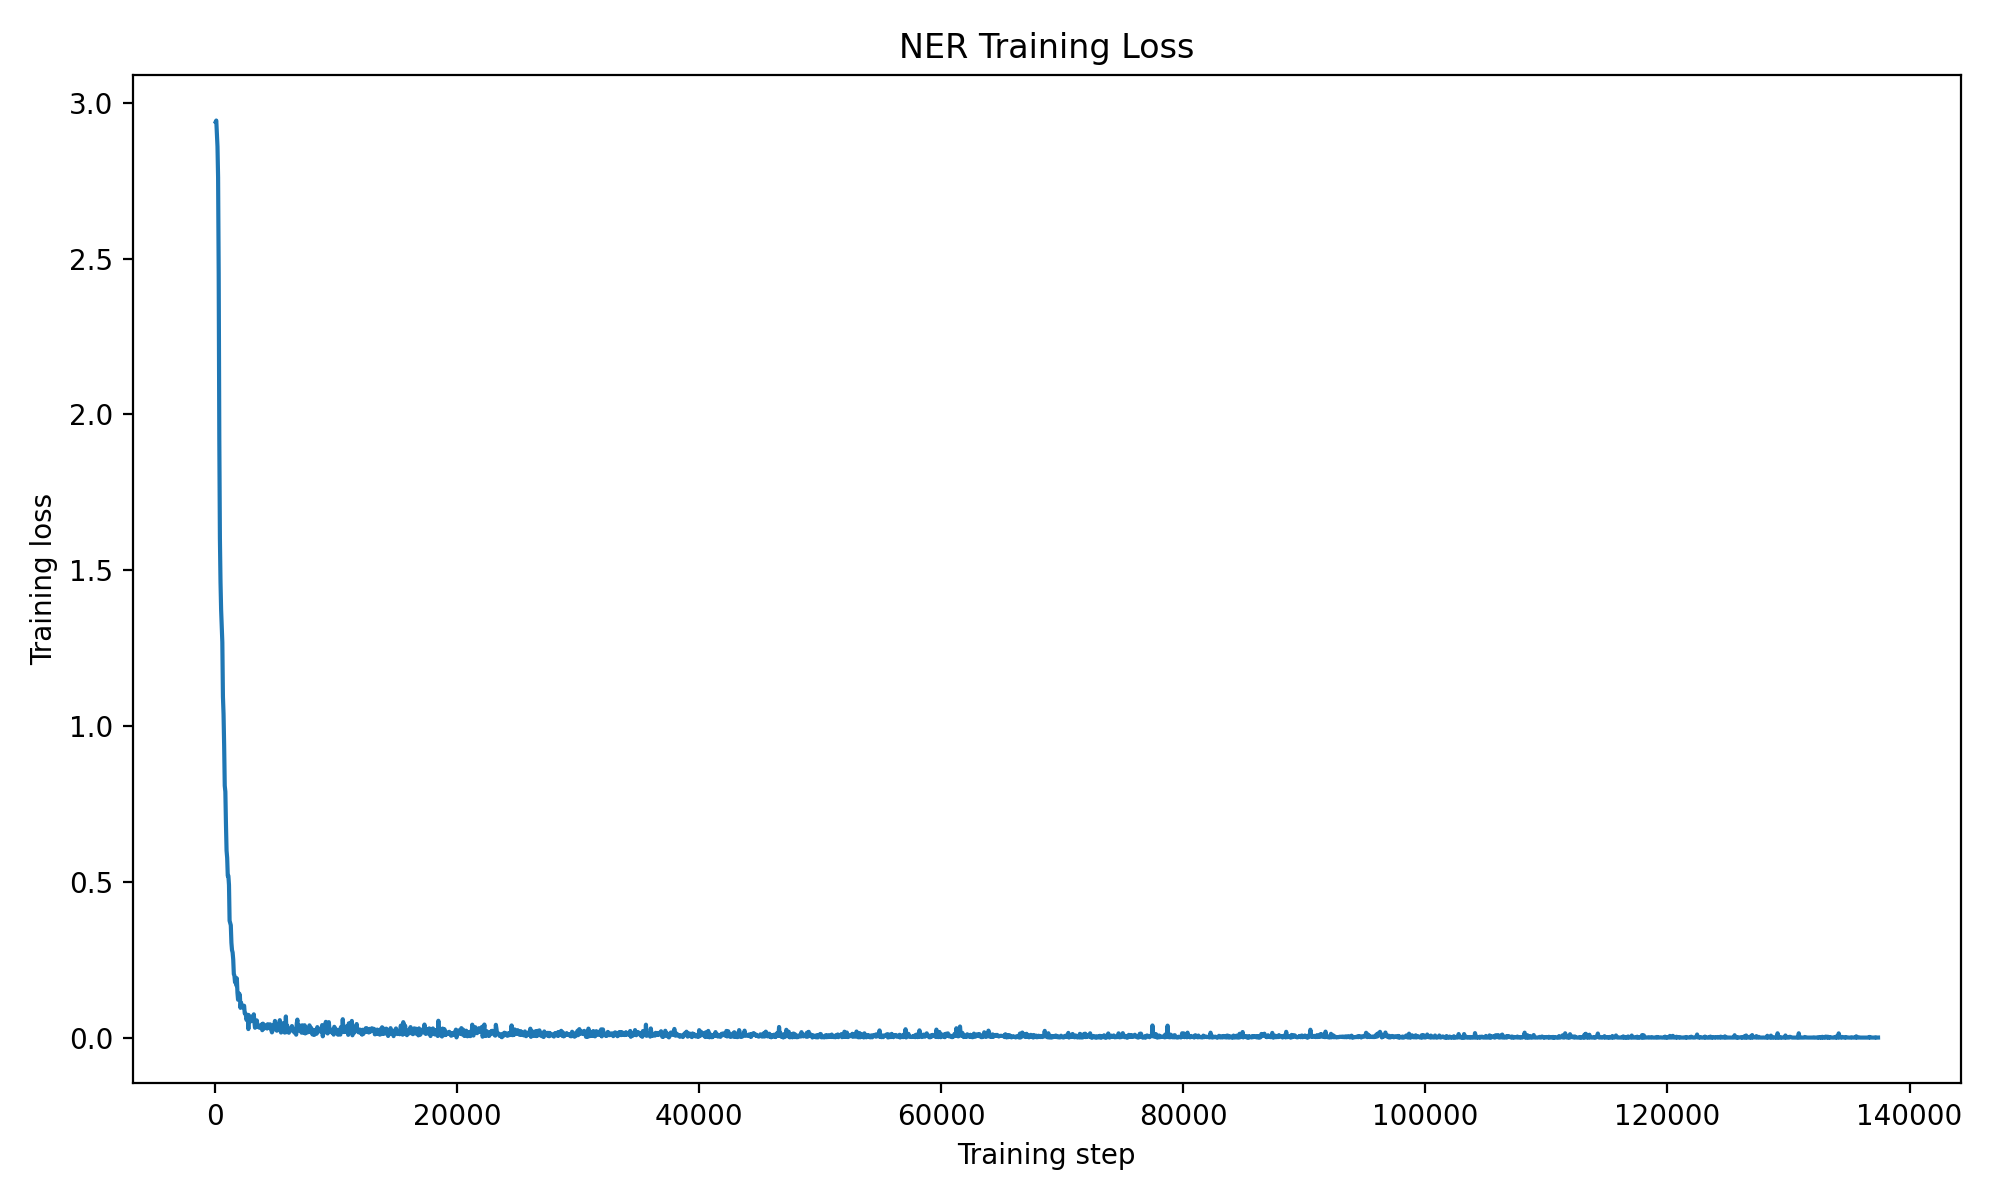
\includegraphics[width=0.82\textwidth]{figures/images/chapter-11/ner/ner_train_loss.png}
\caption{Training loss during fine-tuning of the NER model.}
\label{fig:ner_train_loss}
\end{figure}

\begin{figure}[H]
\centering
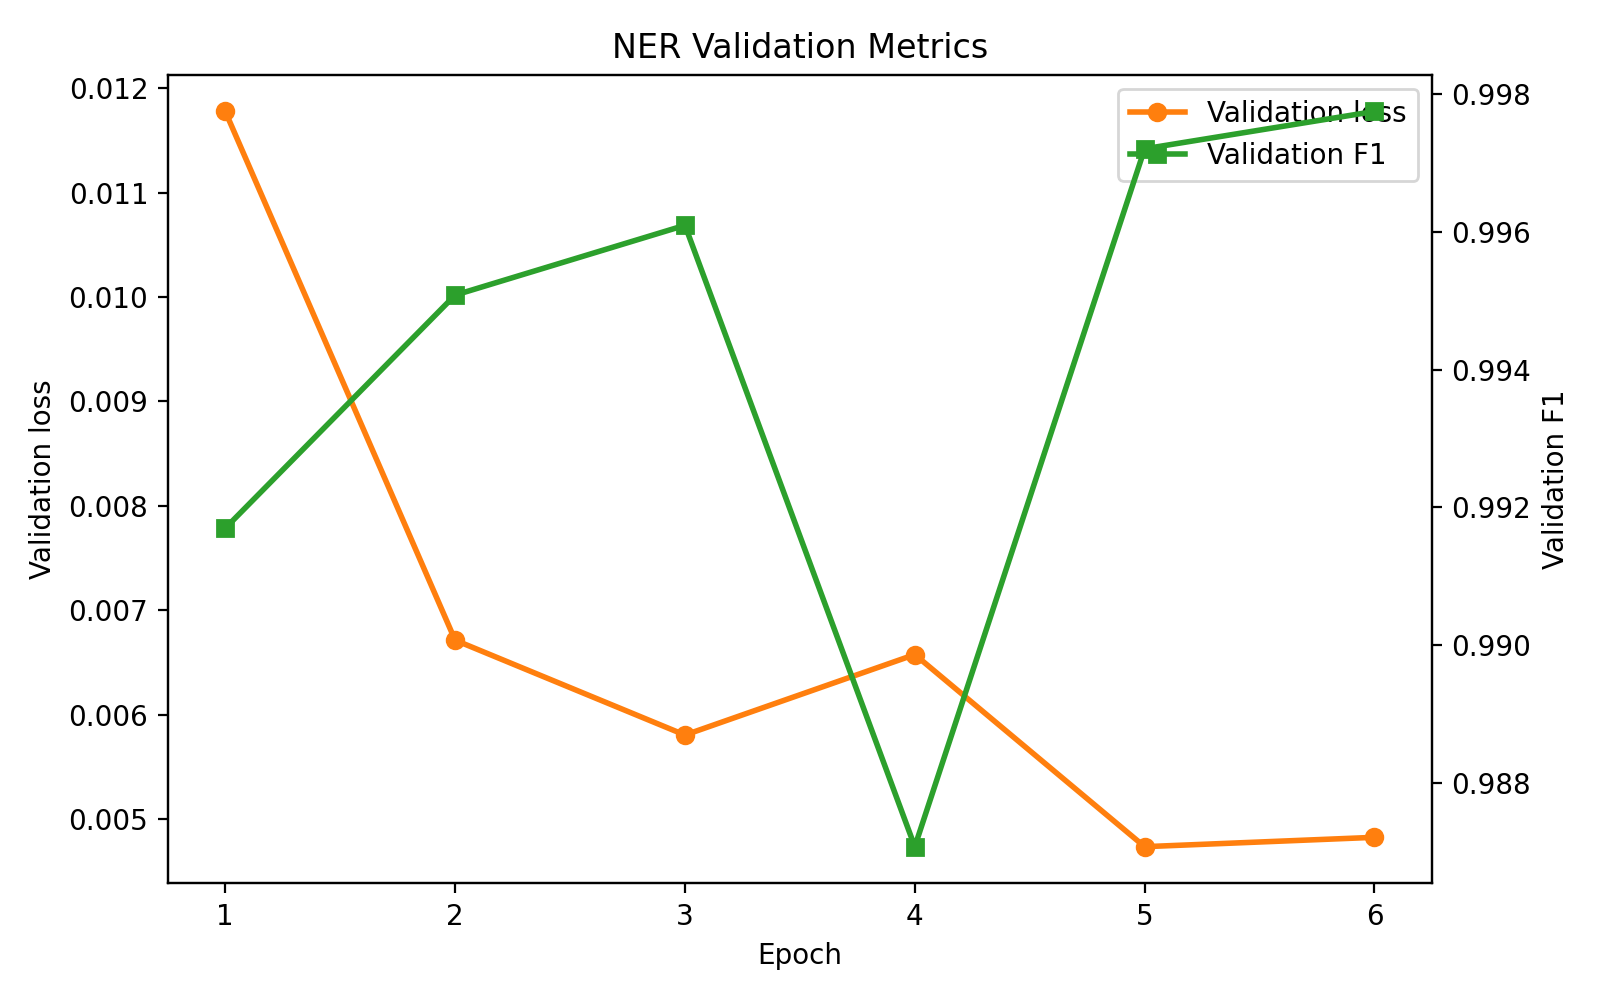
\includegraphics[width=0.78\textwidth]{figures/images/chapter-11/ner/ner_validation_metrics.png}
\caption{Validation loss and validation F1 across training epochs for the NER model. Validation loss is shown on the primary y-axis, while validation F1 is shown on the secondary y-axis.}
\label{fig:ner_validation_metrics}
\end{figure}

Taken together, the curves indicate stable convergence on the constructed training
and validation data, but they do not by themselves demonstrate robust performance
on real-world OCR document scenarios.

\subsection{Per-Label Evaluation}

To better assess generalization, the model was also evaluated on a separate harder
OCR-oriented test set. The overall performance on this set is shown in
Table~\ref{tab:ner_results_hard_appendix}, while the per-label performance is shown
in Table~\ref{tab:ner_hard_test_results} and Figure~\ref{fig:ner_per_label_metrics}.

\begin{table}[H]
\centering
\begin{tabular}{lccc}
\toprule
\textbf{Evaluation set} & \textbf{Precision} & \textbf{Recall} & \textbf{F1 Score} \\
\midrule
Hard test set & 91.32\% & 96.13\% & 0.9366 \\
\bottomrule
\end{tabular}
\caption{Overall NER performance on the harder OCR-oriented test set.}
\label{tab:ner_results_hard_appendix}
\end{table}

\begin{table}[H]
\centering
\begin{tabular}{lcccc}
\toprule
\textbf{Label} & \textbf{Precision} & \textbf{Recall} & \textbf{F1 Score} & \textbf{Support} \\
\midrule
ADDRESS        & 100.00\% & 100.00\% & 1.0000 & 37 \\
DATE           & 100.00\% & 100.00\% & 1.0000 & 50 \\
EMAIL          & 100.00\% & 100.00\% & 1.0000 & 83 \\
ID\_NUMBER     & 90.74\%  & 98.00\%  & 0.9423 & 50 \\
LICENSE\_PLATE & 95.45\%  & 100.00\% & 0.9767 & 21 \\
LOCATION       & 84.21\%  & 88.89\%  & 0.8649 & 72 \\
ORGANIZATION   & 67.16\%  & 95.74\%  & 0.7895 & 47 \\
PERSON\_NAME   & 86.21\%  & 93.75\%  & 0.8982 & 80 \\
PHONE          & 100.00\% & 91.43\%  & 0.9552 & 70 \\
POSTAL\_CODE   & 100.00\% & 100.00\% & 1.0000 & 59 \\
\bottomrule
\end{tabular}
\caption{Per-label performance of the NER model on the harder OCR-oriented test set.}
\label{tab:ner_hard_test_results}
\end{table}

\begin{figure}[H]
\centering
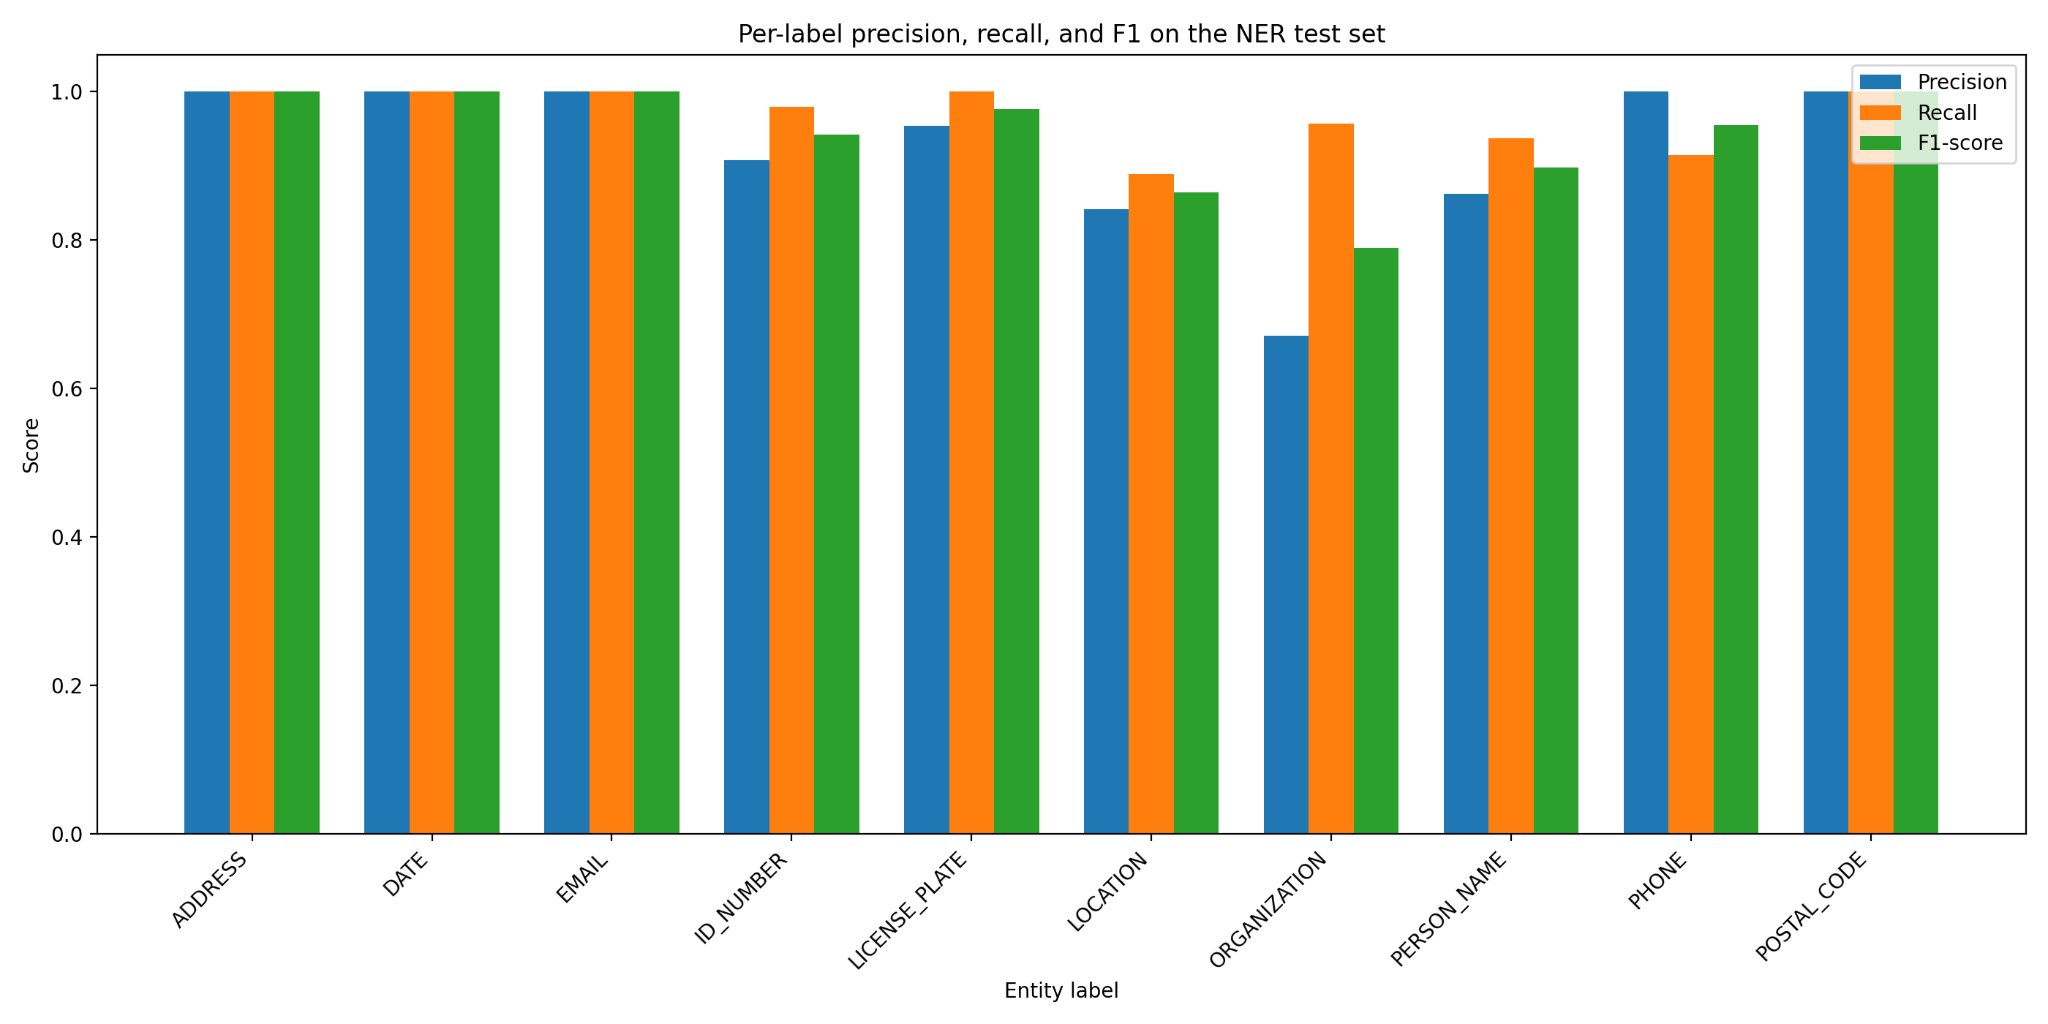
\includegraphics[width=0.9\textwidth]{figures/images/chapter-11/ner/ner_per_label_metrics.png}
\caption{Per-label precision, recall, and F1 on the harder OCR-oriented test set.}
\label{fig:ner_per_label_metrics}
\end{figure}

As shown in Table~\ref{tab:ner_hard_test_results} and
Figure~\ref{fig:ner_per_label_metrics}, the model remained strong on more
structured entity types such as email addresses, postal codes, dates, and
addresses. However, performance was noticeably weaker for semantically more
ambiguous categories such as organizations, locations, and person names. This
indicates that the model generalized less reliably when the OCR text became more
document-oriented and difficult to categorize.

\subsection{Error Analysis}

Figure~\ref{fig:ner_real_vs_controlled } shows a qualitative comparison
between a controlled example and a real-world document scenario. In the
controlled example, the text is more structured and the categorization pipeline
assigns several relevant labels. In the real-world document example, the OCR
text is more fragmented and the assigned categories are less consistent.

These examples illustrate an important limitation of the NER component. While
the model can perform well on structured and simplified inputs, it has greater
difficulty distinguishing reliably between entity categories in practical
document scenarios. This was particularly visible for semantically similar
categories such as person names, organizations, and locations.

\subsection{Summary}

Overall, the NER model achieved very strong results on the constructed held-out
test split and converged stably during training. However, the harder OCR-oriented
evaluation and the qualitative document examples showed that these results
overestimated the practical robustness of the model. In particular, the model
was less reliable for semantically ambiguous categories such as organization,
location, and person-name entities. For this reason, the final SafeVision system
did not rely on the NER model alone, but instead used it as part of a hybrid
text-analysis pipeline.
\chapter{Detailed Video Evaluation Methodology}
\label{app:video_evaluation_details}

This appendix provides additional details and supporting results for the video processing evaluation in Section~\ref{sec:video_processing_results}. Section~\ref{sec:video_processing_results} reports the main system-level results, while this appendix documents the test material, evaluation setup, annotation procedure, metrics, temporal coverage test, and additional failure-case analysis.

\section{Evaluation Setup}

The video evaluation was performed as a system-level extension of the image detection and redaction pipeline. The tests focused on detection frequency, automatic prediction, and manual tracking. They were performed on three short videos with different resolutions, orientations, and durations. Each video was processed using different values of \texttt{detect\_every}, where lower values run detection more frequently and higher values rely more on prediction between detection frames.

\begin{table}[H]
\centering
\begin{tabular}{lcccc}
\toprule
\textbf{Video} & \textbf{Resolution} & \textbf{Frames} & \textbf{Duration} & \textbf{\acrshort{fps}} \\
\midrule
car\_video & $1280\times720$ & 153 & 5.10 s & 30.00 \\
walk & $854\times480$ & 360 & 12.00 s & 30.00 \\
face\_track & $720\times1280$ & 270 & 9.14 s & 29.55 \\
\bottomrule
\end{tabular}
\caption{Overview of videos used for evaluating the video processing pipeline.}
\label{tab:video_test_material}
\end{table}

The evaluation focused on three main aspects. First, automatic Kalman-based prediction was evaluated to determine whether propagated \gls{bounding box}es remained accurate between detection frames. Second, manual tracking was evaluated to determine whether a user-selected object could be followed across a video sequence. Third, processing performance was measured to evaluate how different detection intervals affected runtime.

\section{Ground-Truth Annotation}

Automatic prediction was evaluated by comparing the generated frame-wise manifests with human-labeled ground-truth boxes. The \texttt{detect\_every = 1} configuration was used as a full-detection baseline, but it was excluded from the Kalman prediction accuracy results because no intermediate non-detection frames exist in this configuration. Since every frame receives detector output, the Kalman filter does not need to estimate object positions between detection frames in this case.

For the remaining configurations, predicted boxes were compared with human-labeled boxes on non-detection frames. These frames are important because they represent cases where the system relies on Kalman prediction instead of new detector output.

For manual tracking, the car was first manually annotated on sampled frames across the \texttt{car\_video} video. The manual tracker was then initialized from a ground-truth box in the middle of the video, and the predicted boxes were compared with the human-labeled boxes using \acrshort{iou}.

\section{Evaluation Metrics}

The evaluation used \acrshort{iou} and sensitive-region coverage as the main accuracy metrics.

\paragraph{Intersection over Union}

\acrshort{iou} measures how closely the predicted box aligns with the human-labeled box. It is calculated as the overlap between the predicted and ground-truth boxes divided by their union.

\[
IoU = \frac{Area(B_p \cap B_g)}{Area(B_p \cup B_g)}
\]

where \(B_p\) represents the predicted box and \(B_g\) represents the ground-truth box.

\paragraph{Sensitive-Region Coverage}

Sensitive-region coverage measures how much of the human-labeled sensitive region was covered by the predicted box. This metric was included because anonymization does not only depend on tight localization. A box can be slightly less precise but still cover the sensitive content sufficiently for redaction.

\section{Temporal Coverage Test}

Before evaluating prediction accuracy against human-labeled ground truth, a temporal coverage test was performed. The purpose of this test was not to measure exact tracking accuracy, but to measure whether Kalman-based prediction preserved active \gls{bounding box}es across frames where full detection was not executed.

Since full detection is only executed on selected frames, a detection-only manifest would only contain detected boxes on those frames. Automatic Kalman-based prediction was therefore compared with this detection-frame-only estimate to evaluate whether it preserved the \gls{bounding box}es across non-detection frames.

\begin{table}[H]
\centering
\begin{tabular}{rccc}
\toprule
\textbf{\texttt{detect\_every}} & \textbf{Detection calls} & \textbf{Detection-only} & \textbf{Manifest with prediction} \\
\midrule
1  & 261.00 & 99.44\% & 99.44\% \\
2  & 130.67 & 50.02\% & 99.63\% \\
5  & 52.33  & 20.09\% & 99.63\% \\
10 & 26.33  & 10.15\% & 99.17\% \\
\bottomrule
\end{tabular}
\caption{Average frame coverage across the three tested videos. ``Detection-only'' estimates the percentage of frames that would contain boxes if boxes were only used on frames where full detection was executed. ``Manifest with prediction'' shows the percentage of frames with active boxes after Kalman-based prediction has propagated boxes between detection frames.}
\label{tab:video_temporal_coverage}
\end{table}

Kalman-based prediction substantially increased bounding-box coverage when detection was run less frequently. With \texttt{detect\_every = 10}, the detection-frame estimate was 10.15\%, while the prediction-based manifest maintained 99.17\% coverage on average. This confirms that the prediction step filled the gaps between detection frames and produced continuous boxes for later review and redaction.

However, this metric should be interpreted only as a temporal coverage result. It shows whether boxes were present in the frame-wise manifest, but it does not show whether the boxes were accurately aligned with the sensitive objects. For this reason, the main video evaluation in Section~\ref{sec:video_processing_results} uses human-labeled ground truth, \acrshort{iou}, and sensitive-region coverage as the primary accuracy results.

\section{Processing-Time Benchmark Setup}

Processing performance was evaluated using the same \texttt{detect\_every} values as the prediction accuracy evaluation. Each configuration was run three times after a warmup run, and the reported values were averaged across the three tested videos. The benchmark was executed on CPU.

The measured processing time included the complete video processing path used in the evaluation, including frame decoding, selected frame-level detection calls, prediction between detection frames, and manifest generation. The purpose of the benchmark was to measure how reducing the number of detection calls affected total processing cost.

\section{Worst-Frame Example}

Figure~\ref{fig:video_prediction_worst_frame} shows the lowest-quality frame found in the \texttt{car\_video} sequence when using \texttt{detect\_every = 10}. This example was selected from the human-labeled evaluation and illustrates a difficult case with several nearby moving vehicles.

\begin{figure}[H]
\centering
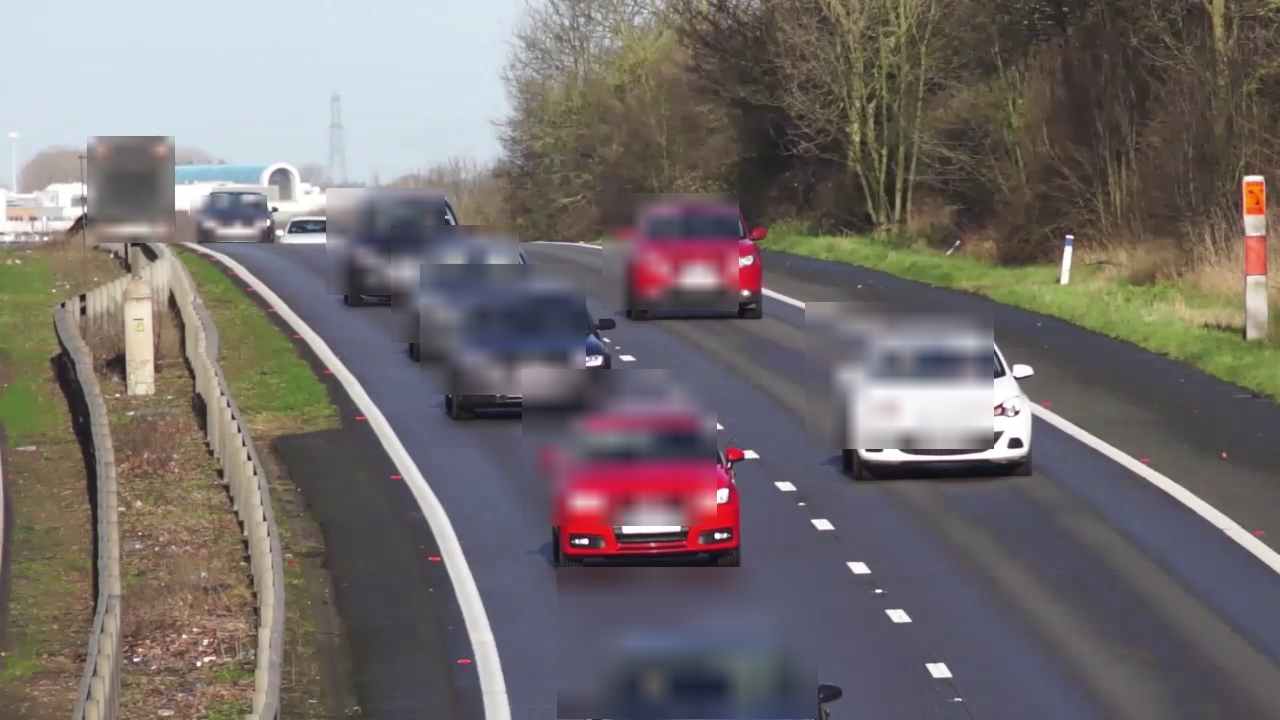
\includegraphics[width=0.85\textwidth]{figures/images/chapter-11/car_kalman_worst_frame.png}
\caption{Worst-frame example from the \texttt{car\_video} sequence using \texttt{detect\_every = 10}. The frame contained nine human-labeled vehicle boxes and ten predicted boxes. The mean \acrshort{iou} was 0.5245, while mean sensitive-region coverage was 0.7469. This illustrates that long prediction intervals can reduce localization accuracy in frames with several nearby moving objects.}
\label{fig:video_prediction_worst_frame}
\end{figure}

This example shows why both \acrshort{iou} and sensitive-region coverage were used in the main evaluation. The predicted boxes still cover large parts of the sensitive regions, but the alignment is less precise than in easier frames. This makes the frame useful as a qualitative example of the limitations of longer prediction intervals.

The lower \acrshort{iou} in this frame was mainly caused by several nearby moving vehicles that produced overlapping prediction paths between sparse detection frames. This type of scenario is more challenging for prediction than isolated objects with stable movement. The example supports the main result that \texttt{detect\_every = 10} provides the largest runtime reduction, but also increases the risk of localization drift in crowded or fast-moving scenes.
\chapter{Training Configuration Details}
\label{app:yolox_config}

\section{QR and Barcode Detection Model}

\begin{lstlisting}[caption={YOLOX experiment file for QR and barcode detection}, label={lst:yolox_barcode}]
"""
YOLOX experiment configuration for QR and barcode detection.

This configuration defines the training setup used for the custom
barcode detection model. The model is based on the YOLOX-S architecture
and trained on a merged dataset containing both real and synthetic data.

The configuration includes dataset paths, training parameters, and
augmentation settings used during training.
"""

from yolox.exp import Exp as MyExp
from yolox.data import COCODataset, TrainTransform, ValTransform
import os


class Exp(MyExp):
    def __init__(self):
        super(Exp, self).__init__()

        # Experiment name
        self.exp_name = "barcode_merged_yolox_s"

        # --------------------------------------------------
        # Model configuration (YOLOX-S)
        # --------------------------------------------------
        self.depth = 0.33
        self.width = 0.50
        self.num_classes = 1  # Single class: barcode / QR / visual code

        # --------------------------------------------------
        # Dataset configuration
        # --------------------------------------------------
        self.data_dir = os.path.abspath(
            os.path.join(os.path.dirname(__file__), "../../../../barcodeV2/dataset_merged")
        )

        # Annotation files (COCO format)
        self.train_ann = "instances_train2017.json"
        self.val_ann = "instances_test2017.json"  # Used for evaluation

        # Image directories
        self.train_name = "train2017"
        self.val_name = "test2017"

        # --------------------------------------------------
        # Training configuration
        # --------------------------------------------------
        self.max_epoch = 200
        self.data_num_workers = 4

        # Higher resolution improves detection of small barcodes
        # but increases GPU memory usage
        self.input_size = (960, 960)
        self.test_size = (960, 960)

        self.print_interval = 20
        self.eval_interval = 1

        # --------------------------------------------------
        # Data augmentation configuration
        # --------------------------------------------------
        # Mosaic and MixUp disabled due to already diverse dataset
        self.mosaic_prob = 0.0
        self.mixup_prob = 0.0

        # Moderate online augmentations
        self.hsv_prob = 0.5        # Color jitter
        self.flip_prob = 0.5       # Horizontal flip

        # Geometric transformations (kept small to preserve structure)
        self.degrees = 5.0
        self.translate = 0.05
        self.shear = 1.0

    def get_dataset(self, cache=False, cache_type=None):
        """
        Returns the training dataset using COCO format.
        """
        return COCODataset(
            data_dir=self.data_dir,
            json_file=self.train_ann,
            name=self.train_name,
            img_size=self.input_size,
            preproc=TrainTransform(
                max_labels=120,
                flip_prob=self.flip_prob,
                hsv_prob=self.hsv_prob,
            ),
            cache=cache,
            cache_type=cache_type,
        )

    def get_eval_dataset(self, testdev=False, legacy=False, **kwargs):
        """
        Returns the evaluation dataset.
        """
        return COCODataset(
            data_dir=self.data_dir,
            json_file=self.val_ann,
            name=self.val_name,
            img_size=self.test_size,
            preproc=ValTransform(legacy=legacy),
        )
\end{lstlisting}

\section{License Plate Detection Model}

\begin{lstlisting}[caption={YOLOX experiment file for license plate detection}, label={lst:yolox_licenseplate}]
"""
YOLOX experiment configuration for license plate detection.

This configuration defines the training and evaluation setup for the
license plate detection model. The model is based on YOLOX-S and trained
on a custom dataset with COCO-style annotations.

Compared to the barcode model, this configuration uses more aggressive
data augmentation (e.g., mosaic) to improve generalization.
"""

#!/usr/bin/env python3
# -*- coding:utf-8 -*-

import os
import torch
from yolox.exp import Exp as MyExp
from yolox.data import COCODataset, ValTransform
from yolox.evaluators import COCOEvaluator


class Exp(MyExp):
    def __init__(self):
        super().__init__()

        # Experiment name
        self.exp_name = "yolox_s_license_plate"

        # --------------------------------------------------
        # Model configuration (YOLOX-S)
        # --------------------------------------------------
        self.depth = 0.33
        self.width = 0.50
        self.num_classes = 1  # Single class: license plate

        # --------------------------------------------------
        # Dataset configuration
        # --------------------------------------------------
        self.data_dir = os.path.abspath(
            os.path.join(os.path.dirname(__file__), "../../../../license_plate_detection/dataset")
        )

        self.train_ann = "train.json"
        self.val_ann = "test.json"  # Used only for evaluation

        # --------------------------------------------------
        # Training configuration
        # --------------------------------------------------
        self.input_size = (960, 960)
        self.test_size = (960, 960)

        self.max_epoch = 200
        self.no_aug_epochs = 15

        # Learning rate schedule
        self.basic_lr_per_img = 0.01 / 64.0
        self.min_lr_ratio = 0.05
        self.warmup_epochs = 5

        self.data_num_workers = 2
        self.print_interval = 20
        self.eval_interval = 1

        # --------------------------------------------------
        # Data augmentation configuration
        # --------------------------------------------------
        # Mosaic enabled to improve generalization
        self.mosaic_scale = (0.5, 1.5)
        self.mosaic_prob = 0.8

        # MixUp disabled
        self.mixup_prob = 0.0
        self.enable_mixup = False

        # Standard augmentations
        self.hsv_prob = 0.5
        self.flip_prob = 0.5

        # Geometric transformations
        self.degrees = 5.0
        self.translate = 0.05
        self.shear = 1.0

        # Multi-scale training
        self.random_size = (14, 24)

        # --------------------------------------------------
        # Evaluation settings
        # --------------------------------------------------
        self.test_conf = 0.01
        self.nmsthre = 0.65

        self.output_dir = "./YOLOX_outputs"

    def get_eval_loader(self, batch_size, is_distributed, testdev=False, legacy=False):
        """
        Creates the evaluation data loader.
        """
        image_folder = "test2017" if self.val_ann == "test.json" else "val2017"

        valdataset = COCODataset(
            data_dir=self.data_dir,
            json_file=self.val_ann,
            name=image_folder,
            img_size=self.test_size,
            preproc=ValTransform(legacy=legacy),
        )

        if is_distributed:
            batch_size = batch_size // torch.distributed.get_world_size()
            sampler = torch.utils.data.distributed.DistributedSampler(
                valdataset, shuffle=False
            )
        else:
            sampler = torch.utils.data.SequentialSampler(valdataset)

        return torch.utils.data.DataLoader(
            valdataset,
            batch_size=batch_size,
            sampler=sampler,
            num_workers=self.data_num_workers,
            pin_memory=True,
        )

    def get_evaluator(self, batch_size, is_distributed, testdev=False, legacy=False):
        """
        Returns the COCO evaluator used for model evaluation.
        """
        return COCOEvaluator(
            dataloader=self.get_eval_loader(batch_size, is_distributed, testdev, legacy),
            img_size=self.test_size,
            confthre=self.test_conf,
            nmsthre=self.nmsthre,
            num_classes=self.num_classes,
            testdev=testdev,
        )
\end{lstlisting}
\chapter{Hybrid Text Analysis Pipeline}
\label{app:pii_detector}

In the deployed system, OCR-extracted text was not classified by the NER model
alone. Instead, the final text categorization step was implemented through a
hybrid pipeline in \texttt{pii\_detector.py}, where NER predictions were
combined with rule-based checks, contextual field hints, and post-processing
filters. Listings~\ref{lst:pii_detector_extract} and
\ref{lst:pii_detector_rules} show the central extraction logic and an example of
the rule-based entity detection used in the final system.

\begin{lstlisting}[language=Python, caption={Core hybrid extraction logic used after OCR text recognition}, label={lst:pii_detector_extract}]
def extract_entities(
    text: str,
    expected_label: Optional[str] = None,
) -> List[TextEntity]:
    clean = normalize_text(text)
    if not clean:
        return []

    all_rule_ents: List[TextEntity] = []
    all_gliner_ents: List[TextEntity] = []
    all_custom_ents: List[TextEntity] = []

    all_rule_ents.extend(detect_rule_entities(clean, expected_label))
    all_custom_ents.extend(detect_custom_ner_entities(clean, expected_label))
    all_gliner_ents.extend(detect_gliner_entities(clean, expected_label))

    for line in split_lines(clean):
        key, value = extract_key_value(line)
        line_expected = context_label_from_key(key) or expected_label
        segment = value if key else line

        if not segment or is_noise(segment):
            continue

        all_rule_ents.extend(detect_rule_entities(segment, line_expected))
        all_custom_ents.extend(detect_custom_ner_entities(segment, line_expected))
        all_gliner_ents.extend(detect_gliner_entities(segment, line_expected))

        # ... context-based helper rules omitted ...

    entities = merge_all(all_rule_ents, all_gliner_ents, all_custom_ents)

    if (
        not entities
        and expected_label in {"POSTAL_CODE", "PHONE", "ID_NUMBER", "DATE"}
        and len(clean) >= 2
        and not is_noise(clean)
    ):
        entities = [TextEntity(clean, expected_label, 0.50, "context")]

    return dedupe_entities(entities)
\end{lstlisting}

\begin{lstlisting}[language=Python, caption={Example of rule-based entity detection used alongside NER}, label={lst:pii_detector_rules}]
def detect_rule_entities(
    text: str,
    expected_label: Optional[str] = None,
) -> List[TextEntity]:
    t = normalize_token(text)
    entities: List[TextEntity] = []

    if is_noise(t):
        return entities

    for m in EMAIL_RE.finditer(t):
        entities.append(TextEntity(m.group(0), "EMAIL", 0.99, "regex"))

    if NOR_PHONE_RE.fullmatch(t) and is_valid_phone(t):
        entities.append(TextEntity(t, "PHONE", 0.97, "rule"))
    elif expected_label == "PHONE":
        for m in GENERIC_PHONE_RE.finditer(t):
            if is_valid_phone(m.group(0)):
                entities.append(TextEntity(m.group(0), "PHONE", 0.90, "regex+context"))

    if POSTAL_RE.fullmatch(t):
        entities.append(TextEntity(t, "POSTAL_CODE", 0.96, "rule"))

    if looks_like_date(t):
        entities.append(TextEntity(t, "DATE", 0.93, "rule"))

    # ... additional rules omitted ...

    return dedupe_entities(entities)
\end{lstlisting}

Listing~\ref{lst:pii_detector_extract} shows that the final text-analysis
component combined multiple sources of evidence rather than relying only on the
NER model. Listing~\ref{lst:pii_detector_rules} illustrates how structured
entity types such as email addresses, phone numbers, postal codes, and dates
were reinforced through explicit rules in addition to model-based predictions.
\chapter{Detailed Test Coverage}
\label{app:test_cov_detailed}


\section{Frontend Coverage Report}
\label{appendix:frontend_coverage_full}

% Auto-generated from coverage/coverage-final.json
\footnotesize
\begin{longtable}{>{\raggedright\arraybackslash}p{0.72\textwidth}rrr}
\hline
\textbf{File} & \textbf{Stmts} & \textbf{Miss} & \textbf{Cover} \\
\hline
\endfirsthead
\hline
\textbf{File} & \textbf{Stmts} & \textbf{Miss} & \textbf{Cover} \\
\hline
\endhead
src/\allowbreak App.tsx & 5 & 0 & 100.00\% \\
src/\allowbreak app/\allowbreak AppShell.tsx & 19 & 15 & 21.05\% \\
src/\allowbreak app/\allowbreak useAppController.ts & 36 & 4 & 88.89\% \\
src/\allowbreak features/\allowbreak detection/\allowbreak components/\allowbreak CategoryMultiSelect.tsx & 45 & 27 & 40.00\% \\
src/\allowbreak features/\allowbreak detection/\allowbreak components/\allowbreak DetectionFiltersSection.tsx & 26 & 8 & 69.23\% \\
src/\allowbreak features/\allowbreak detection/\allowbreak domain/\allowbreak detectionFilters.logic.ts & 25 & 18 & 28.00\% \\
src/\allowbreak features/\allowbreak detection/\allowbreak domain/\allowbreak detectionGroups.ts & 2 & 0 & 100.00\% \\
src/\allowbreak features/\allowbreak detection/\allowbreak domain/\allowbreak detectionMapping.ts & 7 & 3 & 57.14\% \\
src/\allowbreak features/\allowbreak detection/\allowbreak domain/\allowbreak detectionSelection.logic.ts & 14 & 5 & 64.29\% \\
src/\allowbreak features/\allowbreak detection/\allowbreak hooks/\allowbreak useDetectionFilters.ts & 2 & 1 & 50.00\% \\
src/\allowbreak features/\allowbreak detection/\allowbreak state/\allowbreak detectionFiltersStore.ts & 31 & 2 & 93.55\% \\
src/\allowbreak features/\allowbreak file/\allowbreak component/\allowbreak FilePanel.tsx & 52 & 44 & 15.38\% \\
src/\allowbreak features/\allowbreak file/\allowbreak component/\allowbreak Sidebar.tsx & 32 & 21 & 34.38\% \\
src/\allowbreak features/\allowbreak file/\allowbreak context/\allowbreak FileTaskProgressContext.tsx & 2 & 0 & 100.00\% \\
src/\allowbreak features/\allowbreak file/\allowbreak context/\allowbreak FileTaskProgressContextValue.ts & 1 & 0 & 100.00\% \\
src/\allowbreak features/\allowbreak file/\allowbreak context/\allowbreak FileTaskProgressTypes.ts & 0 & 0 & 100.00\% \\
src/\allowbreak features/\allowbreak file/\allowbreak hooks/\allowbreak useFileActions.ts & 77 & 20 & 74.03\% \\
src/\allowbreak features/\allowbreak file/\allowbreak hooks/\allowbreak useFileDelete.ts & 11 & 9 & 18.18\% \\
src/\allowbreak features/\allowbreak file/\allowbreak hooks/\allowbreak useFileSelection.ts & 74 & 27 & 63.51\% \\
src/\allowbreak features/\allowbreak file/\allowbreak hooks/\allowbreak useFileTaskProgress.ts & 2 & 0 & 100.00\% \\
src/\allowbreak features/\allowbreak file/\allowbreak hooks/\allowbreak useFileUpload.ts & 19 & 17 & 10.53\% \\
src/\allowbreak features/\allowbreak file/\allowbreak hooks/\allowbreak useHistoryAwareStores.ts & 44 & 13 & 70.45\% \\
src/\allowbreak features/\allowbreak file/\allowbreak hooks/\allowbreak useTaskProgressManagement.ts & 20 & 11 & 45.00\% \\
src/\allowbreak features/\allowbreak file/\allowbreak model/\allowbreak fileClipboard.ts & 32 & 5 & 84.38\% \\
src/\allowbreak features/\allowbreak file/\allowbreak model/\allowbreak reorderImages.ts & 18 & 16 & 11.11\% \\
src/\allowbreak features/\allowbreak highlights/\allowbreak components/\allowbreak HighlightColorChip.tsx & 3 & 3 & 0.00\% \\
src/\allowbreak features/\allowbreak userPreference/\allowbreak components/\allowbreak StylesPanel.tsx & 49 & 25 & 48.98\% \\
src/\allowbreak features/\allowbreak userPreference/\allowbreak components/\allowbreak UserPreferencePanel.tsx & 2 & 0 & 100.00\% \\
src/\allowbreak features/\allowbreak userPreference/\allowbreak context/\allowbreak UserPreferencesContext.ts & 1 & 0 & 100.00\% \\
src/\allowbreak features/\allowbreak userPreference/\allowbreak context/\allowbreak UserPreferencesProvider.tsx & 5 & 0 & 100.00\% \\
src/\allowbreak features/\allowbreak userPreference/\allowbreak context/\allowbreak UserPreferencesTypes.ts & 0 & 0 & 100.00\% \\
src/\allowbreak features/\allowbreak userPreference/\allowbreak hooks/\allowbreak useApplyTheme.ts & 33 & 19 & 42.42\% \\
src/\allowbreak features/\allowbreak userPreference/\allowbreak hooks/\allowbreak useEditorShortcuts.ts & 18 & 15 & 16.67\% \\
src/\allowbreak features/\allowbreak userPreference/\allowbreak hooks/\allowbreak useGlobalShortcuts.ts & 35 & 25 & 28.57\% \\
src/\allowbreak features/\allowbreak userPreference/\allowbreak hooks/\allowbreak useTaskProgress.ts & 32 & 4 & 87.50\% \\
src/\allowbreak features/\allowbreak userPreference/\allowbreak hooks/\allowbreak useUserPreferences.ts & 4 & 1 & 75.00\% \\
src/\allowbreak features/\allowbreak userPreference/\allowbreak hooks/\allowbreak useUserPreferencesState.ts & 52 & 27 & 48.08\% \\
src/\allowbreak features/\allowbreak userPreference/\allowbreak index.ts & 0 & 0 & 100.00\% \\
src/\allowbreak features/\allowbreak userPreference/\allowbreak model/\allowbreak userPreferences.ts & 1 & 0 & 100.00\% \\
src/\allowbreak features/\allowbreak userPreference/\allowbreak utils/\allowbreak highlightStyle.ts & 9 & 0 & 100.00\% \\
src/\allowbreak features/\allowbreak userPreference/\allowbreak utils/\allowbreak shortcut.ts & 36 & 3 & 91.67\% \\
src/\allowbreak features/\allowbreak workspace/\allowbreak components/\allowbreak ContextMenu.tsx & 11 & 4 & 63.64\% \\
src/\allowbreak features/\allowbreak workspace/\allowbreak components/\allowbreak DragOverlay.tsx & 3 & 1 & 66.67\% \\
src/\allowbreak features/\allowbreak workspace/\allowbreak components/\allowbreak WorkspaceEmptyState.tsx & 1 & 0 & 100.00\% \\
src/\allowbreak features/\allowbreak workspace/\allowbreak hooks/\allowbreak state/\allowbreak useWorkspaceAIMission.ts & 13 & 10 & 23.08\% \\
src/\allowbreak features/\allowbreak workspace/\allowbreak hooks/\allowbreak state/\allowbreak useWorkspaceRedaction.ts & 115 & 102 & 11.30\% \\
src/\allowbreak features/\allowbreak workspace/\allowbreak hooks/\allowbreak useCanvasHover.ts & 15 & 11 & 26.67\% \\
src/\allowbreak features/\allowbreak workspace/\allowbreak hooks/\allowbreak useHighlightBoxEditor.ts & 125 & 108 & 13.60\% \\
src/\allowbreak features/\allowbreak workspace/\allowbreak hooks/\allowbreak useVisibleHighlights.ts & 2 & 0 & 100.00\% \\
src/\allowbreak features/\allowbreak workspace/\allowbreak hooks/\allowbreak useWorkspaceFileDrop.ts & 36 & 2 & 94.44\% \\
src/\allowbreak features/\allowbreak workspace/\allowbreak media/\allowbreak image/\allowbreak ImageWorkspace.tsx & 135 & 106 & 21.48\% \\
src/\allowbreak features/\allowbreak workspace/\allowbreak media/\allowbreak image/\allowbreak components/\allowbreak CanvasSurface.tsx & 72 & 72 & 0.00\% \\
src/\allowbreak features/\allowbreak workspace/\allowbreak media/\allowbreak image/\allowbreak components/\allowbreak PageEditorSurface.tsx & 55 & 28 & 49.09\% \\
src/\allowbreak features/\allowbreak workspace/\allowbreak media/\allowbreak image/\allowbreak hooks/\allowbreak boxClipboard.ts & 6 & 1 & 83.33\% \\
src/\allowbreak features/\allowbreak workspace/\allowbreak media/\allowbreak image/\allowbreak hooks/\allowbreak useCanvasImage.ts & 32 & 32 & 0.00\% \\
src/\allowbreak features/\allowbreak workspace/\allowbreak media/\allowbreak image/\allowbreak hooks/\allowbreak useImageAIMission.ts & 91 & 35 & 61.54\% \\
src/\allowbreak features/\allowbreak workspace/\allowbreak media/\allowbreak image/\allowbreak hooks/\allowbreak useImageBoxes.ts & 56 & 37 & 33.93\% \\
src/\allowbreak features/\allowbreak workspace/\allowbreak media/\allowbreak image/\allowbreak hooks/\allowbreak useImageEditor.ts & 14 & 14 & 0.00\% \\
src/\allowbreak features/\allowbreak workspace/\allowbreak media/\allowbreak image/\allowbreak hooks/\allowbreak useImageRedaction.ts & 53 & 53 & 0.00\% \\
src/\allowbreak features/\allowbreak workspace/\allowbreak media/\allowbreak video/\allowbreak VideoCanvasOverlay.tsx & 229 & 155 & 32.31\% \\
src/\allowbreak features/\allowbreak workspace/\allowbreak media/\allowbreak video/\allowbreak VideoWorkspace.tsx & 101 & 100 & 0.99\% \\
src/\allowbreak features/\allowbreak workspace/\allowbreak media/\allowbreak video/\allowbreak hooks/\allowbreak useVideoAIMission.ts & 43 & 43 & 0.00\% \\
src/\allowbreak features/\allowbreak workspace/\allowbreak media/\allowbreak video/\allowbreak hooks/\allowbreak useVideoObjectUrls.ts & 26 & 26 & 0.00\% \\
src/\allowbreak features/\allowbreak workspace/\allowbreak media/\allowbreak video/\allowbreak hooks/\allowbreak useVideoPlaybackState.ts & 179 & 24 & 86.59\% \\
src/\allowbreak features/\allowbreak workspace/\allowbreak media/\allowbreak video/\allowbreak hooks/\allowbreak useVideoRedaction.ts & 37 & 37 & 0.00\% \\
src/\allowbreak features/\allowbreak workspace/\allowbreak media/\allowbreak video/\allowbreak utils/\allowbreak videoDetectionOptions.ts & 46 & 1 & 97.83\% \\
src/\allowbreak features/\allowbreak workspace/\allowbreak media/\allowbreak video/\allowbreak utils/\allowbreak videoManifest.ts & 77 & 18 & 76.62\% \\
src/\allowbreak features/\allowbreak workspace/\allowbreak utils/\allowbreak \_\_testUtils\_\_/\allowbreak rect.ts & 1 & 0 & 100.00\% \\
src/\allowbreak features/\allowbreak workspace/\allowbreak utils/\allowbreak canvasExporter.ts & 84 & 63 & 25.00\% \\
src/\allowbreak features/\allowbreak workspace/\allowbreak utils/\allowbreak detectionLabel.ts & 23 & 9 & 60.87\% \\
src/\allowbreak features/\allowbreak workspace/\allowbreak utils/\allowbreak rectHitTest.ts & 45 & 9 & 80.00\% \\
src/\allowbreak features/\allowbreak workspace/\allowbreak utils/\allowbreak rectTransform.ts & 13 & 0 & 100.00\% \\
src/\allowbreak features/\allowbreak workspace/\allowbreak utils/\allowbreak workspaceHandle.ts & 0 & 0 & 100.00\% \\
src/\allowbreak hooks/\allowbreak effects/\allowbreak useAIMissionProgress.ts & 42 & 10 & 76.19\% \\
src/\allowbreak hooks/\allowbreak state/\allowbreak useDetectionsStore.ts & 23 & 0 & 100.00\% \\
src/\allowbreak hooks/\allowbreak state/\allowbreak useEditorHistory.ts & 27 & 0 & 100.00\% \\
src/\allowbreak hooks/\allowbreak state/\allowbreak useHighlightsForImage.ts & 27 & 27 & 0.00\% \\
src/\allowbreak hooks/\allowbreak state/\allowbreak useHighlightsStore.ts & 57 & 2 & 96.49\% \\
src/\allowbreak hooks/\allowbreak state/\allowbreak useImages.ts & 32 & 0 & 100.00\% \\
src/\allowbreak hooks/\allowbreak state/\allowbreak useUndoRedoHistory.ts & 78 & 7 & 91.03\% \\
src/\allowbreak hooks/\allowbreak state/\allowbreak useVideoManifestStore.ts & 62 & 16 & 74.19\% \\
src/\allowbreak hooks/\allowbreak ui/\allowbreak useCloseOnEscapeAndOutsideClick.ts & 19 & 1 & 94.74\% \\
src/\allowbreak hooks/\allowbreak ui/\allowbreak useConsentGate.ts & 52 & 7 & 86.54\% \\
src/\allowbreak hooks/\allowbreak ui/\allowbreak useContextMenu.ts & 20 & 6 & 70.00\% \\
src/\allowbreak hooks/\allowbreak ui/\allowbreak useCtrlDragPan.ts & 47 & 25 & 46.81\% \\
src/\allowbreak hooks/\allowbreak ui/\allowbreak useMediaQuery.ts & 15 & 2 & 86.67\% \\
src/\allowbreak hooks/\allowbreak ui/\allowbreak usePreventBrowserZoom.ts & 14 & 1 & 92.86\% \\
src/\allowbreak hooks/\allowbreak ui/\allowbreak useSidebarState.ts & 15 & 3 & 80.00\% \\
src/\allowbreak hooks/\allowbreak ui/\allowbreak useTopbarFit.ts & 34 & 20 & 41.18\% \\
src/\allowbreak hooks/\allowbreak ui/\allowbreak useVideoFullscreenProxy.ts & 64 & 7 & 89.06\% \\
src/\allowbreak hooks/\allowbreak ui/\allowbreak useViewportWheelZoom.ts & 30 & 22 & 26.67\% \\
src/\allowbreak hooks/\allowbreak ui/\allowbreak useZoom.ts & 16 & 0 & 100.00\% \\
src/\allowbreak lib/\allowbreak canvas/\allowbreak canvasDraw.ts & 55 & 54 & 1.82\% \\
src/\allowbreak main.tsx & 1 & 1 & 0.00\% \\
src/\allowbreak models/\allowbreak detectionCategories.ts & 10 & 0 & 100.00\% \\
src/\allowbreak models/\allowbreak detectionFilters.ts & 35 & 8 & 77.14\% \\
src/\allowbreak models/\allowbreak image.ts & 0 & 0 & 100.00\% \\
src/\allowbreak models/\allowbreak imageDocumentId.ts & 5 & 5 & 0.00\% \\
src/\allowbreak models/\allowbreak imageInstance.ts & 12 & 12 & 0.00\% \\
src/\allowbreak models/\allowbreak rect.ts & 0 & 0 & 100.00\% \\
src/\allowbreak models/\allowbreak redaction.ts & 0 & 0 & 100.00\% \\
src/\allowbreak services/\allowbreak detection/\allowbreak detectionApi.ts & 17 & 17 & 0.00\% \\
src/\allowbreak services/\allowbreak http/\allowbreak abortError.ts & 3 & 3 & 0.00\% \\
src/\allowbreak services/\allowbreak http/\allowbreak apiClient.ts & 1 & 0 & 100.00\% \\
src/\allowbreak services/\allowbreak http/\allowbreak httpClient.ts & 26 & 26 & 0.00\% \\
src/\allowbreak services/\allowbreak redaction/\allowbreak redactionApi.ts & 14 & 14 & 0.00\% \\
src/\allowbreak services/\allowbreak storage/\allowbreak browserStorageKeys.ts & 38 & 8 & 78.95\% \\
src/\allowbreak services/\allowbreak storage/\allowbreak editorIndexedDb.ts & 43 & 35 & 18.60\% \\
src/\allowbreak services/\allowbreak storage/\allowbreak highlightsIndexedDbRepository.ts & 64 & 56 & 12.50\% \\
src/\allowbreak services/\allowbreak storage/\allowbreak highlightsRepository.ts & 0 & 0 & 100.00\% \\
src/\allowbreak services/\allowbreak storage/\allowbreak userPreferencesRepository.ts & 53 & 5 & 90.57\% \\
src/\allowbreak services/\allowbreak storage/\allowbreak videoManifestIndexedDbRepository.ts & 31 & 30 & 3.23\% \\
src/\allowbreak services/\allowbreak storage/\allowbreak videoManifestRepository.ts & 0 & 0 & 100.00\% \\
src/\allowbreak shared/\allowbreak utils/\allowbreak cx.ts & 1 & 0 & 100.00\% \\
src/\allowbreak shared/\allowbreak utils/\allowbreak fileKey.ts & 33 & 7 & 78.79\% \\
src/\allowbreak ui/\allowbreak components/\allowbreak ConsentGateModal.tsx & 12 & 4 & 66.67\% \\
src/\allowbreak ui/\allowbreak components/\allowbreak FilePicker.tsx & 9 & 7 & 22.22\% \\
src/\allowbreak ui/\allowbreak components/\allowbreak FileRowProgress.tsx & 6 & 0 & 100.00\% \\
src/\allowbreak ui/\allowbreak components/\allowbreak GlowRing.tsx & 2 & 2 & 0.00\% \\
src/\allowbreak ui/\allowbreak components/\allowbreak PatchNotesModal.tsx & 23 & 13 & 43.48\% \\
src/\allowbreak ui/\allowbreak components/\allowbreak SearchInput.tsx & 2 & 1 & 50.00\% \\
src/\allowbreak ui/\allowbreak components/\allowbreak ToggleSwitch.tsx & 4 & 2 & 50.00\% \\
src/\allowbreak ui/\allowbreak components/\allowbreak ToolBarButtons.tsx & 5 & 1 & 80.00\% \\
src/\allowbreak ui/\allowbreak components/\allowbreak Tooltip.tsx & 22 & 17 & 22.73\% \\
src/\allowbreak ui/\allowbreak components/\allowbreak UploadDropzone.tsx & 2 & 2 & 0.00\% \\
src/\allowbreak ui/\allowbreak components/\allowbreak WorkspaceProgressBar.tsx & 4 & 4 & 0.00\% \\
src/\allowbreak ui/\allowbreak components/\allowbreak common/\allowbreak CanvasTooltip.tsx & 3 & 3 & 0.00\% \\
src/\allowbreak ui/\allowbreak components/\allowbreak common/\allowbreak HighlightColorChipView.tsx & 2 & 2 & 0.00\% \\
src/\allowbreak ui/\allowbreak components/\allowbreak sidebar/\allowbreak IconRail.tsx & 5 & 0 & 100.00\% \\
src/\allowbreak ui/\allowbreak components/\allowbreak sidebar/\allowbreak SidePanelResizeHandleView.tsx & 2 & 0 & 100.00\% \\
src/\allowbreak ui/\allowbreak components/\allowbreak sidebar/\allowbreak SidePanelShell.tsx & 2 & 0 & 100.00\% \\
src/\allowbreak ui/\allowbreak components/\allowbreak sidebar/\allowbreak SidePanelTypes.ts & 0 & 0 & 100.00\% \\
src/\allowbreak ui/\allowbreak components/\allowbreak sidebar/\allowbreak SidebarView.tsx & 5 & 0 & 100.00\% \\
src/\allowbreak ui/\allowbreak components/\allowbreak sidebar/\allowbreak panels/\allowbreak filePanel/\allowbreak DropIndicator.tsx & 3 & 3 & 0.00\% \\
src/\allowbreak ui/\allowbreak components/\allowbreak sidebar/\allowbreak panels/\allowbreak filePanel/\allowbreak FilePanelItemRowView.tsx & 25 & 15 & 40.00\% \\
src/\allowbreak ui/\allowbreak components/\allowbreak sidebar/\allowbreak panels/\allowbreak filePanel/\allowbreak FilePanelView.tsx & 39 & 12 & 69.23\% \\
src/\allowbreak ui/\allowbreak components/\allowbreak sidebar/\allowbreak panels/\allowbreak filePanel/\allowbreak filePanelDnd.ts & 29 & 29 & 0.00\% \\
src/\allowbreak ui/\allowbreak components/\allowbreak sidebar/\allowbreak panels/\allowbreak filePanel/\allowbreak filePanelGrouping.ts & 2 & 2 & 0.00\% \\
src/\allowbreak ui/\allowbreak components/\allowbreak sidebar/\allowbreak panels/\allowbreak filePanel/\allowbreak filePanelTypes.ts & 1 & 1 & 0.00\% \\
src/\allowbreak ui/\allowbreak components/\allowbreak sidebar/\allowbreak panels/\allowbreak filePanel/\allowbreak filePanelUtils.ts & 1 & 1 & 0.00\% \\
src/\allowbreak ui/\allowbreak components/\allowbreak sidebar/\allowbreak panels/\allowbreak settingsPanel/\allowbreak CategoryMultiSelectView.tsx & 41 & 31 & 24.39\% \\
src/\allowbreak ui/\allowbreak components/\allowbreak sidebar/\allowbreak panels/\allowbreak settingsPanel/\allowbreak DetectionFiltersSectionView.tsx & 2 & 0 & 100.00\% \\
src/\allowbreak ui/\allowbreak components/\allowbreak sidebar/\allowbreak panels/\allowbreak settingsPanel/\allowbreak SettingsPanel.tsx & 29 & 16 & 44.83\% \\
src/\allowbreak ui/\allowbreak components/\allowbreak sidebar/\allowbreak panels/\allowbreak stylesPanel/\allowbreak HighlightStyleEditorView.tsx & 53 & 33 & 37.74\% \\
src/\allowbreak ui/\allowbreak components/\allowbreak sidebar/\allowbreak panels/\allowbreak stylesPanel/\allowbreak StylesPanelView.tsx & 28 & 12 & 57.14\% \\
src/\allowbreak ui/\allowbreak components/\allowbreak sidebar/\allowbreak panels/\allowbreak userPreferencePanel/\allowbreak UserPreferencePanelView.tsx & 38 & 27 & 28.95\% \\
src/\allowbreak ui/\allowbreak components/\allowbreak topbar/\allowbreak RedactionOptionsBar.tsx & 7 & 7 & 0.00\% \\
src/\allowbreak ui/\allowbreak components/\allowbreak topbar/\allowbreak Topbar.tsx & 67 & 32 & 52.24\% \\
src/\allowbreak ui/\allowbreak components/\allowbreak topbar/\allowbreak buildMoreItems.tsx & 11 & 0 & 100.00\% \\
src/\allowbreak ui/\allowbreak components/\allowbreak topbar/\allowbreak topbarLayout.ts & 9 & 0 & 100.00\% \\
\hline
\end{longtable}
\normalsize


























\section{Backend Coverage Report}
\label{appendix:backend_coverage_full}

% Auto-generated from backend_coverage.json
\footnotesize
\begin{longtable}{>{\raggedright\arraybackslash}p{0.72\textwidth}rrr}
\hline
\textbf{File} & \textbf{Stmts} & \textbf{Miss} & \textbf{Cover} \\
\hline
\endfirsthead
\hline
\textbf{File} & \textbf{Stmts} & \textbf{Miss} & \textbf{Cover} \\
\hline
\endhead
backend/\allowbreak \_\_init\_\_.py & 0 & 0 & 100.00\% \\
backend/\allowbreak config/\allowbreak cpu\_runtime.py & 6 & 0 & 100.00\% \\
backend/\allowbreak controllers/\allowbreak \_\_init\_\_.py & 0 & 0 & 100.00\% \\
backend/\allowbreak controllers/\allowbreak detect\_controller.py & 90 & 0 & 100.00\% \\
backend/\allowbreak controllers/\allowbreak redact\_controller.py & 74 & 0 & 100.00\% \\
backend/\allowbreak controllers/\allowbreak video\_detect\_controller.py & 29 & 0 & 100.00\% \\
backend/\allowbreak controllers/\allowbreak video\_redact\_controller.py & 49 & 0 & 100.00\% \\
backend/\allowbreak controllers/\allowbreak video\_track\_manual\_controller.py & 33 & 0 & 100.00\% \\
backend/\allowbreak main.py & 51 & 0 & 100.00\% \\
backend/\allowbreak pipeline/\allowbreak barcode/\allowbreak detection/\allowbreak barcode\_detector.py & 9 & 0 & 100.00\% \\
backend/\allowbreak pipeline/\allowbreak common/\allowbreak detection\_types.py & 12 & 0 & 100.00\% \\
backend/\allowbreak pipeline/\allowbreak common/\allowbreak postprocessing/\allowbreak nms.py & 20 & 0 & 100.00\% \\
backend/\allowbreak pipeline/\allowbreak common/\allowbreak preprocessing/\allowbreak preprocessing.py & 57 & 0 & 100.00\% \\
backend/\allowbreak pipeline/\allowbreak common/\allowbreak preprocessing/\allowbreak rotation.py & 29 & 0 & 100.00\% \\
backend/\allowbreak pipeline/\allowbreak common/\allowbreak redaction/\allowbreak \_\_init\_\_.py & 0 & 0 & 100.00\% \\
backend/\allowbreak pipeline/\allowbreak common/\allowbreak redaction/\allowbreak anonymize.py & 186 & 1 & 99.46\% \\
backend/\allowbreak pipeline/\allowbreak common/\allowbreak redaction/\allowbreak inpaint.py & 56 & 0 & 100.00\% \\
backend/\allowbreak pipeline/\allowbreak common/\allowbreak segmentation/\allowbreak \_\_init\_\_.py & 2 & 0 & 100.00\% \\
backend/\allowbreak pipeline/\allowbreak common/\allowbreak segmentation/\allowbreak mobile\_sam\_segmenter.py & 36 & 0 & 100.00\% \\
backend/\allowbreak pipeline/\allowbreak face/\allowbreak \_\_init\_\_.py & 0 & 0 & 100.00\% \\
backend/\allowbreak pipeline/\allowbreak face/\allowbreak detection/\allowbreak \_\_init\_\_.py & 0 & 0 & 100.00\% \\
backend/\allowbreak pipeline/\allowbreak face/\allowbreak detection/\allowbreak retinaface\_detector.py & 70 & 0 & 100.00\% \\
backend/\allowbreak pipeline/\allowbreak face/\allowbreak detection/\allowbreak retinaface\_loader.py & 8 & 0 & 100.00\% \\
backend/\allowbreak pipeline/\allowbreak frame\_live.py & 128 & 0 & 100.00\% \\
backend/\allowbreak pipeline/\allowbreak licenseplate/\allowbreak detection/\allowbreak licenseplate\_detector.py & 9 & 0 & 100.00\% \\
backend/\allowbreak pipeline/\allowbreak pipeline\_core.py & 66 & 0 & 100.00\% \\
backend/\allowbreak pipeline/\allowbreak text/\allowbreak analysis/\allowbreak category\_mapping.py & 24 & 0 & 100.00\% \\
backend/\allowbreak pipeline/\allowbreak text/\allowbreak analysis/\allowbreak id\_parser.py & 23 & 0 & 100.00\% \\
backend/\allowbreak pipeline/\allowbreak text/\allowbreak analysis/\allowbreak ner\_classifier.py & 54 & 1 & 98.15\% \\
backend/\allowbreak pipeline/\allowbreak text/\allowbreak analysis/\allowbreak pii\_detector.py & 289 & 17 & 94.12\% \\
backend/\allowbreak pipeline/\allowbreak text/\allowbreak analysis/\allowbreak text\_analyzer.py & 19 & 0 & 100.00\% \\
backend/\allowbreak pipeline/\allowbreak text/\allowbreak ocr/\allowbreak paddle\_ocr\_detector.py & 103 & 0 & 100.00\% \\
backend/\allowbreak pipeline/\allowbreak text/\allowbreak ocr/\allowbreak paddle\_ocr\_recognizer.py & 36 & 0 & 100.00\% \\
backend/\allowbreak services/\allowbreak detector\_service.py & 101 & 0 & 100.00\% \\
backend/\allowbreak startup/\allowbreak import\_paths.py & 6 & 0 & 100.00\% \\
backend/\allowbreak startup/\allowbreak runtime\_tuning.py & 21 & 0 & 100.00\% \\
backend/\allowbreak video/\allowbreak \_\_init\_\_.py & 0 & 0 & 100.00\% \\
backend/\allowbreak video/\allowbreak bbox\_utils.py & 50 & 1 & 98.00\% \\
backend/\allowbreak video/\allowbreak ffmpeg\_utils.py & 22 & 0 & 100.00\% \\
backend/\allowbreak video/\allowbreak kalman\_multi\_tracker.py & 254 & 11 & 95.67\% \\
backend/\allowbreak video/\allowbreak manual\_single\_tracker.py & 300 & 3 & 99.00\% \\
backend/\allowbreak video/\allowbreak video\_live.py & 178 & 0 & 100.00\% \\
\hline
\end{longtable}
\normalsize

\chapter{Additional Video Prediction Results}
\label{app:video_prediction_additional_results}

This appendix provides additional results for the video prediction evaluation in Section~\ref{sec:video_processing_results}. The main chapter reports the human-labeled accuracy evaluation using \acrshort{iou} and sensitive-region coverage. The results below are included as supporting material.

\section{Temporal Coverage Test}
Before evaluating prediction accuracy against human-labeled ground truth, a temporal coverage test was performed. The purpose of this test was not to measure exact tracking accuracy, but to measure whether Kalman-based prediction preserved active \gls{bounding box}es across frames where full detection was not executed.

Since full detection is only executed on selected frames, a detection-only manifest would only contain detected boxes on those frames. Automatic Kalman-based prediction was therefore compared with this detection-frame-only estimate to evaluate whether it preserved the \gls{bounding box}es across non-detection frames.

\begin{table}[H]
\centering
\begin{tabular}{rccc}
\toprule
\textbf{\texttt{detect\_every}} & \textbf{Detection calls} & \textbf{Detection-only} & \textbf{Manifest with prediction} \\
\midrule
1  & 261.00 & 99.44\% & 99.44\% \\
2  & 130.67 & 50.02\% & 99.63\% \\
5  & 52.33  & 20.09\% & 99.63\% \\
10 & 26.33  & 10.15\% & 99.17\% \\
\bottomrule
\end{tabular}
\caption{Average frame coverage across the three tested videos. ``Detection-only'' estimates the percentage of frames that would contain boxes if boxes were only used on frames where full detection was executed. ``Manifest with prediction'' shows the percentage of frames with active boxes after Kalman-based prediction has propagated boxes between detection frames.}
\label{tab:video_temporal_coverage_appendix}
\end{table}

This substantially increased bounding-box coverage when detection was run less frequently. With \texttt{detect\_every = 10}, the detection-frame estimate was 10.15\%, while the prediction-based manifest maintained 99.17\% coverage on average. This confirms that the prediction step filled the gaps between detection frames and produced continuous boxes for later review and redaction.

However, this metric should be interpreted only as a temporal coverage result. It shows whether boxes were present in the frame-wise manifest, but it does not show whether the boxes were accurately aligned with the sensitive objects. For this reason, the main video evaluation in Section~\ref{sec:video_processing_results} uses human-labeled ground truth, \acrshort{iou}, and sensitive-region coverage as the primary accuracy results.

\section{Worst-Frame Example}

Figure~\ref{fig:video_prediction_worst_frame_appendix} shows the lowest-quality frame found in the \texttt{car\_video} sequence when using \texttt{detect\_every = 10}. This example was selected from the human-labeled evaluation and illustrates a difficult case with several nearby moving vehicles.

\begin{figure}[H]
\centering
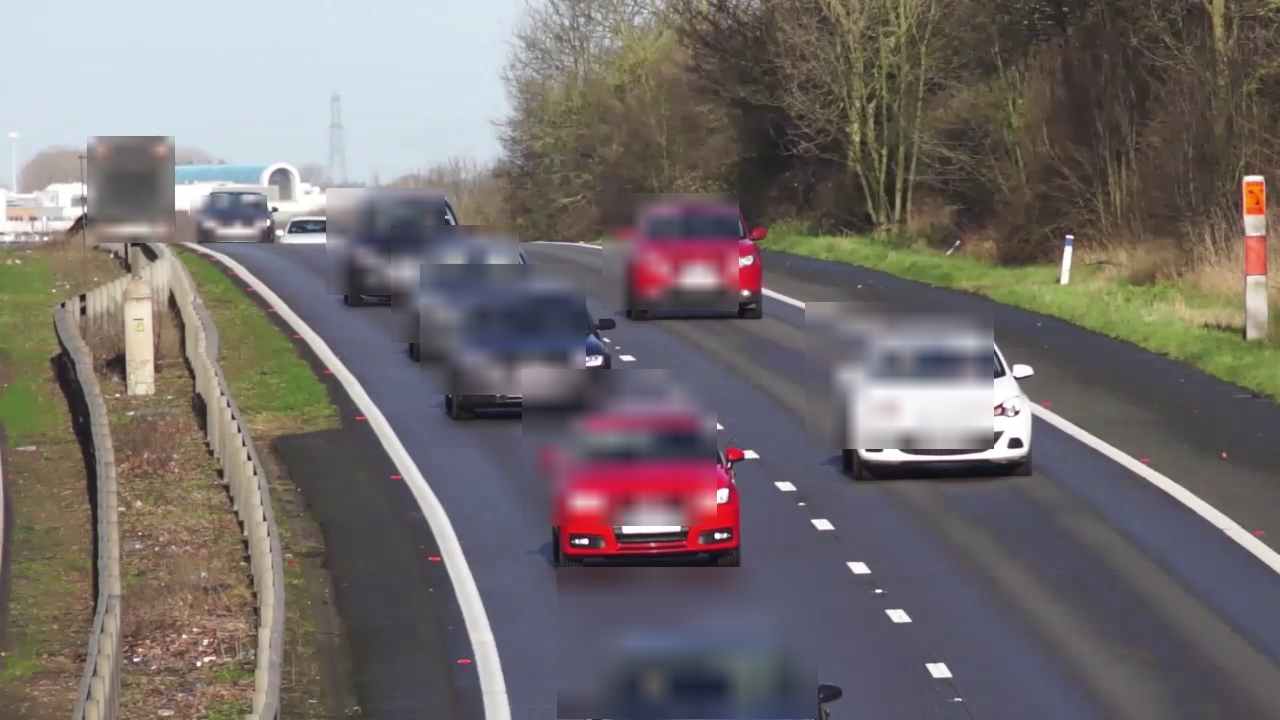
\includegraphics[width=0.85\textwidth]{figures/images/chapter-11/car_kalman_worst_frame.png}
\caption{Worst-frame example from the \texttt{car\_video} sequence using \texttt{detect\_every = 10}. The frame contained nine human-labeled vehicle boxes and ten predicted boxes. The mean \acrshort{iou} was 0.5245, while mean sensitive-region coverage was 0.7469. This illustrates that long prediction intervals can reduce localization accuracy in frames with several nearby moving objects.}
\label{fig:video_prediction_worst_frame_appendix}
\end{figure}

This example shows why both \acrshort{iou} and sensitive-region coverage were used in the main evaluation. The predicted boxes still cover large parts of the sensitive regions, but the alignment is less precise than in easier frames. This makes the frame useful as a qualitative example of the limitations of longer prediction intervals.
% appendices/pen-test.tex

\chapter{Detailed Peneteration Testing and Security Ecaluation}
\label{app:pen_test}

% --------------------------------------------------

\section*{Test 1 --- \texttt{/health} endpoint exposure}

\begin{figure}[h]
    \centering
    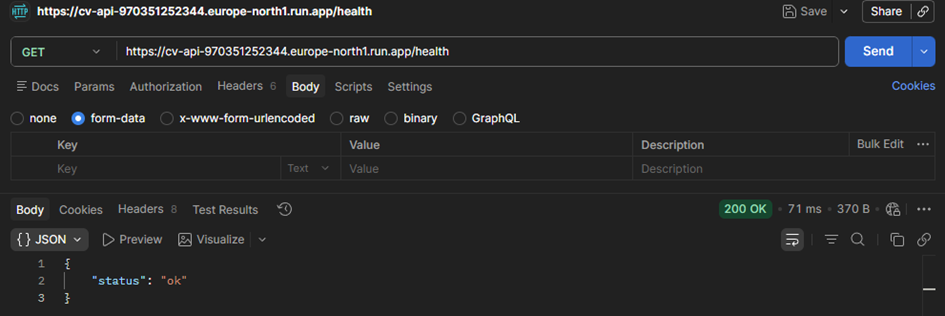
\includegraphics[width=\textwidth]{figures/images/chapter-9/pen-test/health-endpoint-exposure.png}
    \caption{Response from the public \texttt{/health} endpoint}
\end{figure}

\noindent \textbf{Test case:} Public health endpoint inspection

\noindent \textbf{Endpoint:} \texttt{GET /health}

\noindent \textbf{What was sent:} A simple \texttt{GET} request.

\noindent \textbf{Expected result:} A minimal status response without unnecessary internal information.

\noindent \textbf{Actual result:} The endpoint returned \texttt{200 OK} with the minimal JSON response \texttt{\{"status": "ok"\}}. No internal system details, debug data, or sensitive information were exposed.

\noindent \textbf{Assessment:} Worked as expected. The endpoint exposes only minimal health status information and does not appear to leak unnecessary internal data.

% --------------------------------------------------

\section*{Test 1 --- Valid \texttt{/api/detect} request}

\begin{figure}[H]
    \centering
    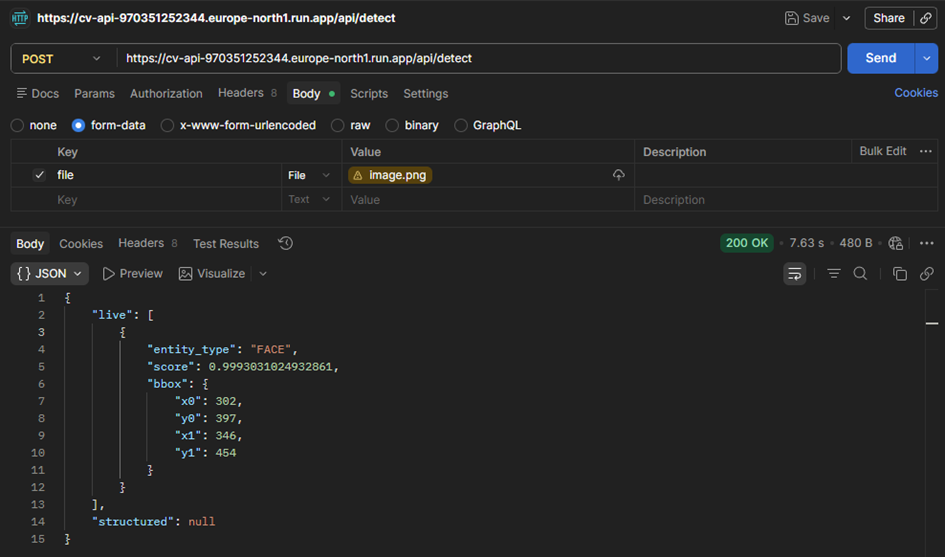
\includegraphics[width=\textwidth]{figures/images/chapter-9/pen-test/valid-api-detect-request.png}
    \caption{Response from a valid request to \texttt{/api/detect}}
\end{figure}

\noindent \textbf{Test case:} Valid image upload to \texttt{/api/detect} 

\noindent \textbf{Endpoint:} \texttt{POST /api/detect} 

\noindent \textbf{What was sent:} A normal image file using multipart form-data. 

\noindent \textbf{Expected result:} The API should return \texttt{200 OK} with detection results. 

\noindent \textbf{Actual result:} The API returned \texttt{200 OK}. The response contained detection output, including \texttt{entity\_type: "FACE"}, a confidence score, and bounding box coordinates. 

\noindent \textbf{Assessment:} Worked as expected. 

% --------------------------------------------------

\section*{Test 2 --- Invalid file disguised as image}

\begin{figure}[H]
    \centering
    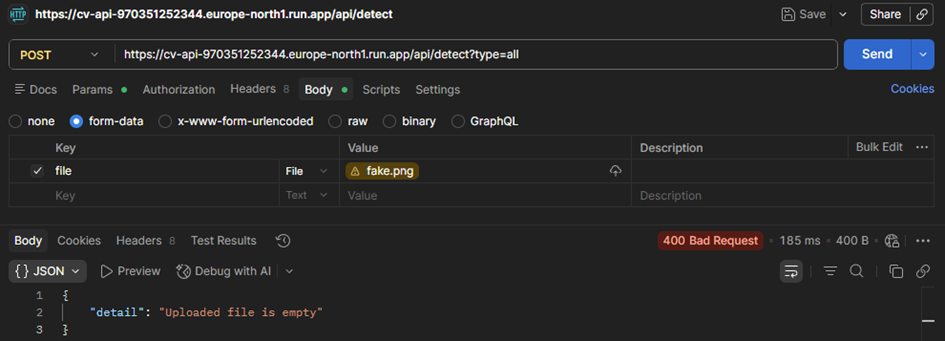
\includegraphics[width=\textwidth]{figures/images/chapter-9/pen-test/fake-image-test.png}
    \caption{Response from invalid file upload to \texttt{/api/detect}}
\end{figure}

\noindent \textbf{Test case:} Invalid file disguised as image 

\noindent \textbf{Endpoint:} \texttt{POST /api/detect} 

\noindent \textbf{What was sent:} An empty text file renamed to \texttt{.jpg} and uploaded as multipart form-data. 

\noindent \textbf{Expected result:} The API should reject the file without crashing and return an appropriate client error response. 

\noindent \textbf{Actual result:} The API returned \texttt{400 Bad Request} with the message \texttt{"Uploaded file is empty"}. 

\noindent \textbf{Assessment:} Worked as expected. The invalid input was handled safely, and the API returned a proper client-side error. 

% --------------------------------------------------

\section*{Test 4 --- Invalid JSON in \texttt{/api/redact}}

\begin{figure}[H]
    \centering
    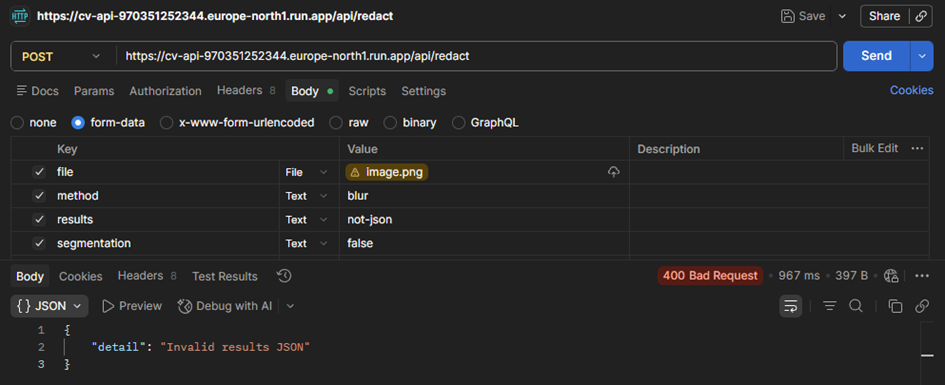
\includegraphics[width=\textwidth]{figures/images/chapter-9/pen-test/redact-invalid-json.png}
    \caption{Response from invalid JSON input to \texttt{/api/redact}}
\end{figure}

\noindent \textbf{Test case:} Invalid JSON in results for \texttt{/api/redact} 

\noindent \textbf{Endpoint:} \texttt{POST /api/redact} 

\noindent \textbf{What was sent:} A valid image, \texttt{method=blur}, \texttt{results=not-json}, and \texttt{segmentation=false}. 

\noindent \textbf{Expected result:} The API should reject the request with a controlled error. 

\noindent \textbf{Actual result:} The API returned \texttt{400 Bad Request} with the message \texttt{"Invalid results JSON"}. 

\noindent \textbf{Assessment:} Worked as expected. The invalid input was handled safely, and the API returned a proper client-side error without crashing. 

% --------------------------------------------------

\section*{Test 6 --- Invalid method in \texttt{/api/redact}}

\begin{figure}[H]
    \centering
    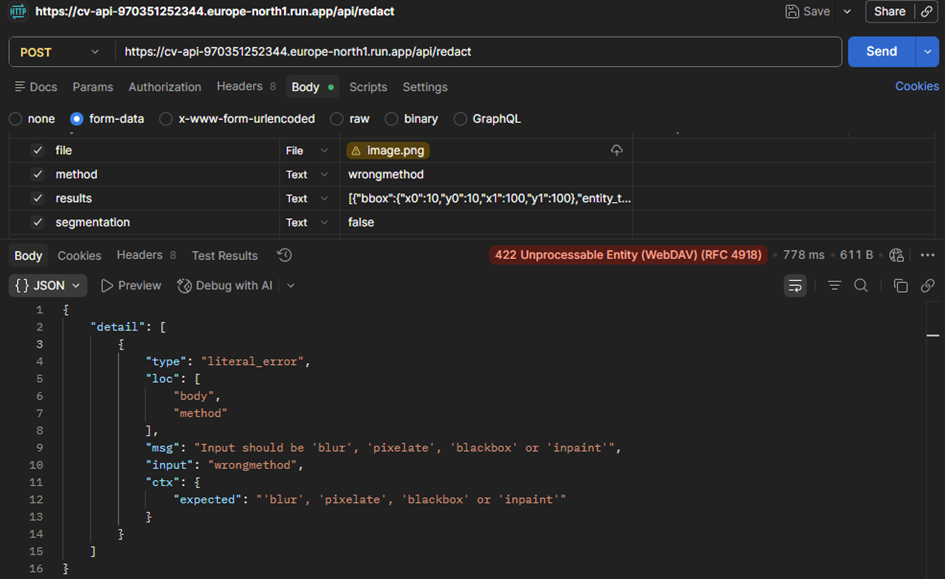
\includegraphics[width=\textwidth]{figures/images/chapter-9/pen-test/invalid-method-redact.png}
    \caption{Response from unsupported method input to \texttt{/api/redact}}
\end{figure}

\noindent \textbf{Test case:} Unsupported redaction method

\noindent \textbf{Endpoint:} \texttt{POST /api/redact}

\noindent \textbf{What was sent:} A valid request with a valid image and results payload, but with \texttt{method=wrongmethod}.

\noindent \textbf{Expected result:} The API should reject the request with a validation error.

\noindent \textbf{Actual result:} The API returned \texttt{422 Unprocessable Entity} with a validation message stating that the input should be \texttt{"blur"}, \texttt{"pixelate"}, \texttt{"blackbox"}, or \texttt{"inpaint"}.

\noindent \textbf{Assessment:} Worked as expected. The invalid method was blocked correctly, and the API returned a controlled validation error without crashing.

% --------------------------------------------------

\section*{Test 7 --- Extreme coordinates in \texttt{/api/redact}}

\begin{figure}[H]
    \centering
    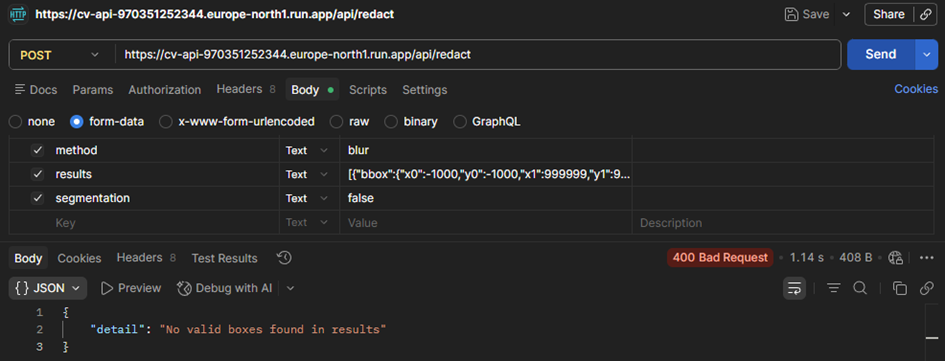
\includegraphics[width=\textwidth]{figures/images/chapter-9/pen-test/extreme-coordinates-redact.png}
    \caption{Response from extreme bounding box coordinates sent to \texttt{/api/redact}}
\end{figure}

\noindent \textbf{Test case:} Extreme bounding box coordinates

\noindent \textbf{Endpoint:} \texttt{POST /api/redact}

\noindent \textbf{What was sent:} A request with very large and negative bounding box coordinates in \texttt{results}: \texttt{[{"bbox":{"x0":-1000,"y0":-1000,"x1":999999,"y1":999999},"entity\_type":"FACE"}]}

\noindent \textbf{Expected result:} The API should handle the request safely without crashing.

\noindent \textbf{Actual result:} The API returned \texttt{400 Bad Request} with the message \texttt{"No valid boxes found in results"}.

\noindent \textbf{Assessment:} Worked as expected. The invalid bounding box coordinates were rejected safely, and the API returned a controlled client-side error without crashing.

% --------------------------------------------------

\section*{Test 10 --- Empty results list on \texttt{/api/redact}}

\begin{figure}[H]
    \centering
    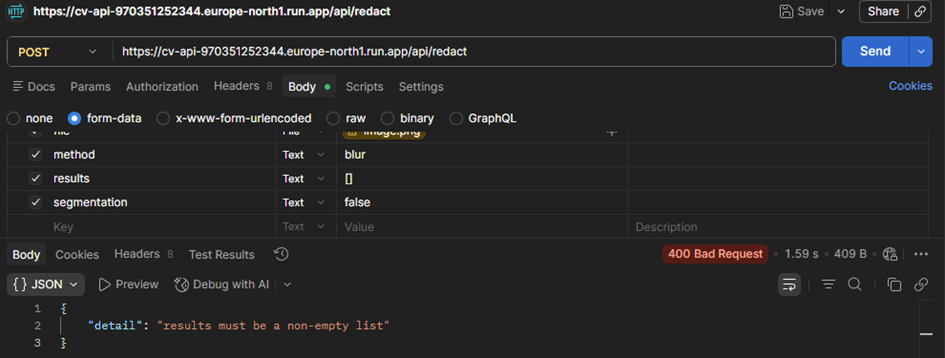
\includegraphics[width=\textwidth]{figures/images/chapter-9/pen-test/empty-results-redact.png}
    \caption{Response from empty \texttt{results} list sent to \texttt{/api/redact}}
\end{figure}

\noindent \textbf{Test case:} Empty results list in \texttt{/api/redact}

\noindent \textbf{Endpoint:} \texttt{POST /api/redact}

\noindent \textbf{What was sent:} A valid image, a valid method, and \texttt{results=[]}.

\noindent \textbf{Expected result:} The API should reject the request with a controlled validation error.

\noindent \textbf{Actual result:} The API returned \texttt{400 Bad Request} with the message \texttt{"results must be a non-empty list"}.

\noindent \textbf{Assessment:} Worked as expected. The empty \texttt{results} list was rejected correctly, and the API returned a controlled client-side error without crashing.

% --------------------------------------------------

\section*{Test 11 --- Malformed results structure on \texttt{/api/redact}}

\begin{figure}[H]
    \centering
    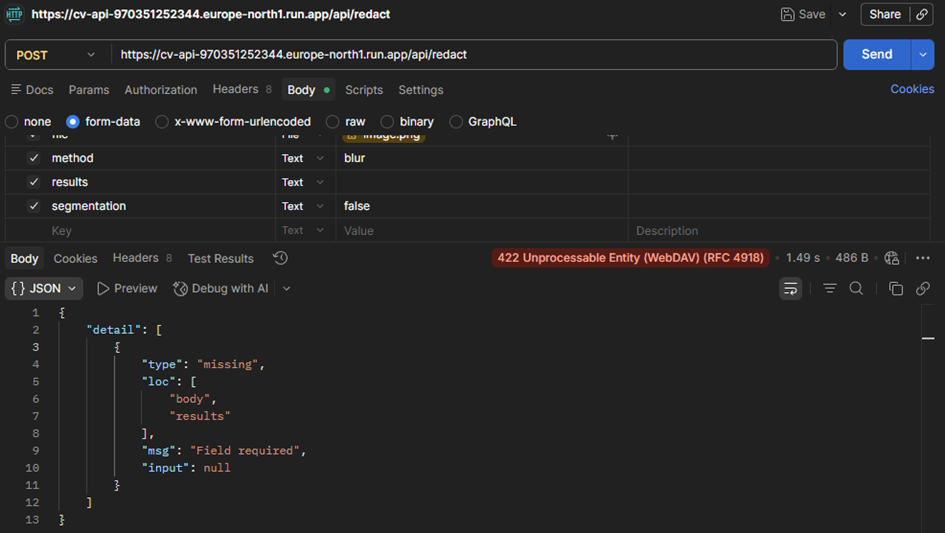
\includegraphics[width=\textwidth]{figures/images/chapter-9/pen-test/malformed-results-redact.png}
    \caption{Response from malformed \texttt{results} input sent to \texttt{/api/redact}}
\end{figure}

\noindent \textbf{Test case:} Malformed results structure in \texttt{/api/redact}

\noindent \textbf{Endpoint:} \texttt{POST /api/redact}

\noindent \textbf{What was sent:} A valid image and valid method, but the \texttt{results} field was malformed and did not contain the required structure. [{"foo":"bar"}]

\noindent \textbf{Expected result:} The API should reject the request or ignore invalid entries safely.

\noindent \textbf{Actual result:} The API returned \texttt{422 Unprocessable Entity} with a validation error stating that the \texttt{results} field was required.

\noindent \textbf{Assessment:} Worked as expected. The malformed input was handled safely, and the API rejected the request with a controlled validation error.

% --------------------------------------------------

\section*{Test 13 --- Many boxes in \texttt{/api/redact}}

\begin{figure}[H]
    \centering
    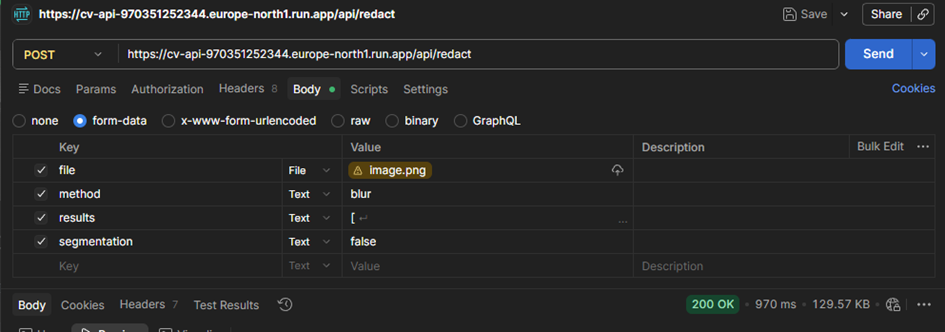
\includegraphics[width=\textwidth]{figures/images/chapter-9/pen-test/many-boxes-redact.png}
    \caption{Response from a \texttt{/api/redact} request with many bounding boxes}
\end{figure}

\noindent \textbf{Test case:} Large number of boxes in \texttt{/api/redact}

\noindent \textbf{Endpoint:} \texttt{POST /api/redact}

\noindent \textbf{What was sent:} A request containing many bounding boxes in the \texttt{results} field. The full payload is not visible in the screenshot because the Postman UI truncates long field values.

\noindent \textbf{Expected result:} The API should remain stable and either complete the request or fail in a controlled way.

\noindent \textbf{Actual result:} The API returned \texttt{200 OK} after approximately \texttt{970 ms}. The request completed successfully and returned a response body of approximately \texttt{129.57 kB}.

\noindent \textbf{Assessment:} Worked as expected. The endpoint remained stable under heavier input and completed the request successfully.

% --------------------------------------------------

\section*{Test 14 --- Invalid query parameters on \texttt{/api/detect}}

\begin{figure}[H]
    \centering
    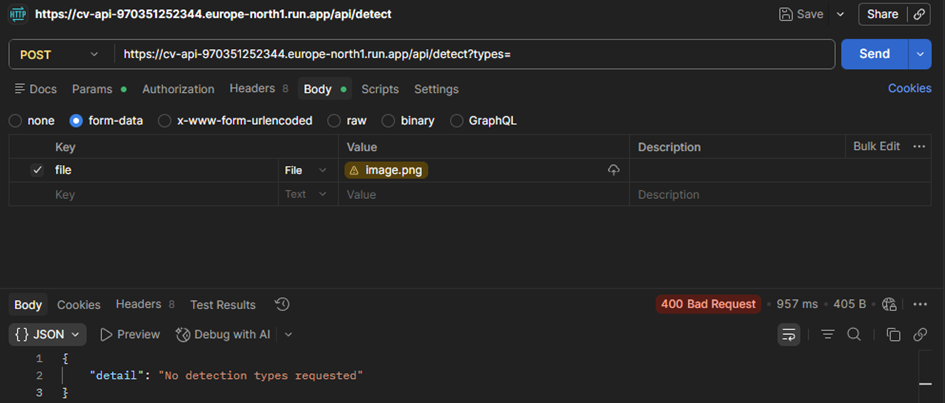
\includegraphics[width=\textwidth]{figures/images/chapter-9/pen-test/invalid-query-parameters-detect.png}
    \caption{Response from invalid query parameters sent to \texttt{/api/detect}}
\end{figure}

\noindent \textbf{Test case:} Invalid query parameters in \texttt{/api/detect}

\noindent \textbf{Endpoint:} \texttt{POST /api/detect}

\noindent \textbf{What was sent:} A request with an empty \texttt{types} query parameter value, shown as \texttt{/api/detect?types=}.

\noindent \textbf{Expected result:} The API should reject invalid parameter combinations safely.

\noindent \textbf{Actual result:} The API returned \texttt{400 Bad Request} with the message \texttt{"No detection types requested"}.

\noindent \textbf{Assessment:} Worked as expected. The invalid query parameter value was handled safely, and the API returned a controlled client-side error without crashing.

% --------------------------------------------------

\section*{Test 23 --- Very large request body / oversized file}

\begin{figure}[h]
    \centering
    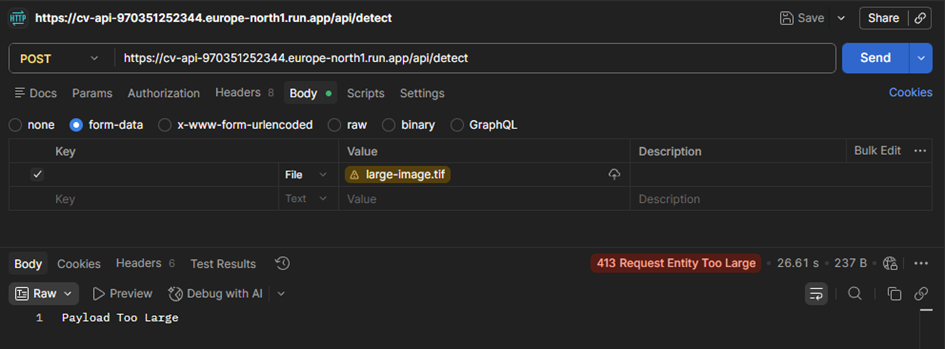
\includegraphics[width=\textwidth]{figures/images/chapter-9/pen-test/oversized-file-detect.png}
    \caption{Response from an oversized file upload sent to \texttt{/api/detect}}
\end{figure}

\noindent \textbf{Test case:} Oversized file upload

\noindent \textbf{Endpoint:} \texttt{POST /api/detect}

\noindent \textbf{What was sent:} A very large image file, shown as \texttt{large-image.tif}.

\noindent \textbf{Expected result:} The API should remain stable and either process the file or fail in a controlled way.

\noindent \textbf{Actual result:} The API returned \texttt{413 Request Entity Too Large} with the message \texttt{Payload Too Large}. The response was returned after approximately \texttt{26.61 s}, so the request was rejected in a controlled way rather than timing out or crashing.

\noindent \textbf{Assessment:} Worked as expected. The oversized upload was handled safely with a controlled error response. However, the response time was relatively high, so upload rejection could potentially be made faster depending on where size validation is enforced.

% --------------------------------------------------



% --------------------------------------------------

\section*{Test 8 --- Browser storage inspection}

\begin{figure}[H]
    \centering
    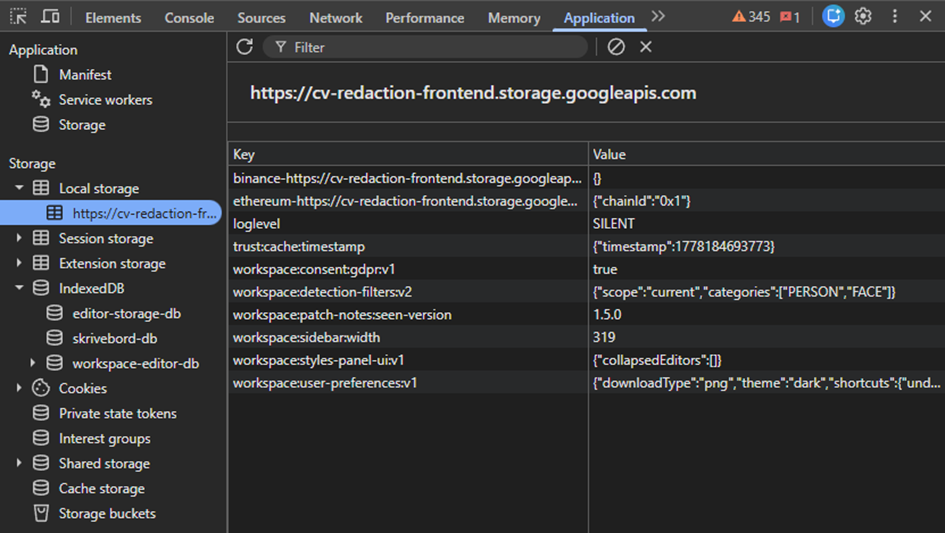
\includegraphics[width=\textwidth]{figures/images/chapter-9/pen-test/browser-storage-inspection.png}
    \caption{Local browser storage entries for the frontend application}
\end{figure}

\noindent \textbf{Test case:} Client-side storage inspection

\noindent \textbf{What was checked:} Browser storage used by the frontend application.

\noindent \textbf{Expected result:} Only local preferences, annotations, or workflow-related state should be stored client-side.

\noindent \textbf{Actual result:} Local storage contained mainly frontend state and preference data, including detection filter settings, consent state, patch notes version, sidebar width, editor UI state, and user preferences such as theme and download type. The view also showed \texttt{binance-...} and \texttt{ethereum-...} entries, which may come from browser wallet integrations or extensions rather than the application itself.

\noindent \textbf{Assessment:} Worked as expected. The stored data appears to be mostly UI preferences and workflow-related client state, which is consistent with a privacy-friendly design. However, this data remains on the client device, and some entries may originate from browser extensions rather than the frontend itself.
% appendices/pen-test.tex

\chapter{Mathematical Model and Verification Script for Redaction Irreversibility}
\label{app:redaction_irreversibility}

This appendix documents the mathematical basis and verification script used for the redaction irreversibility evaluation in Section~\ref{sec:irreversibility-verification}. The purpose is to show why destructive pixel replacement is not reversible from the exported file alone, and to document how the pixel-level verification was performed.

\section{Mathematical Model}

A digital image can be represented as an array or matrix of pixel values. Gonzalez and Woods define an image as a two-dimensional function \(f(x,y)\), where \(x\) and \(y\) are spatial coordinates, and the value of the function represents the image intensity at that point~\cite{gonzalez2018digital}. For colour images, each pixel contains several channel values, such as red, green, and blue in the RGB colour model. The image can therefore be modelled as:

\[
I \in \{0,\ldots,255\}^{H \times W \times C},
\]

where \(H\) is the image height, \(W\) is the image width, and \(C\) is the number of colour channels. For an RGB image, \(C=3\). Let \(R\) denote the region selected for redaction.

A destructive black box redaction function \(F\) produces an exported image \(J\) such that:

\[
J(x,y,c) =
\begin{cases}
k_c, & \text{if } (x,y) \in R, \\
I(x,y,c), & \text{if } (x,y) \notin R,
\end{cases}
\]

where \(k\) is a constant colour value, for example \(k=(0,0,0)\) for black redaction.

This operation removes the original pixel values inside \(R\). The mathematical reason this cannot be reversed uniquely follows from the standard property of inverse functions: a function must be one-to-one in order to have a unique inverse on its image~\cite{rosen2019discrete}. To illustrate this, consider two different original images \(I_1\) and \(I_2\) that are identical outside \(R\), but different inside \(R\). After black box redaction, both images contain the same constant values inside \(R\), and the same unchanged pixels outside \(R\). Therefore,

\[
F(I_1,R) = F(I_2,R)
\]

even though

\[
I_1 \neq I_2.
\]

The function is therefore not injective. Since multiple different original images can produce the same exported redacted image, no unique inverse function exists that can reconstruct the original content from the exported file alone~\cite{rosen2019discrete}. This is consistent with redaction guidance from The National Archives, which states that redaction must irreversibly remove the required information from the redacted copy and remove it from the underlying bitstream rather than only from the visible display~\cite{nationalarchives_redaction_toolkit}. The same principle is also reflected in guidance from the Information Commissioner's Office, which describes the purpose of redaction as irreversibly removing exempt information from the redacted copy~\cite{ico_disclose_safely}.

This irreversibility depends on the original pixels being destructively overwritten and not preserved in hidden layers, metadata, embedded previews, caches, or external copies. For this reason, the verification also included a metadata check. This is aligned with guidance on de-identification and safe disclosure, which treats redaction as a removal-based de-identification technique~\cite{nist800188}. The ICO guidance further illustrates that visually hiding information with a black box is not sufficient if the underlying electronic file still contains the original information~\cite{ico_disclose_safely}.

\begin{lstlisting}[language=Python, caption={Pixel-level verification script for exported redaction}, label={lst:redaction-verification-script}]
from PIL import Image, ExifTags
import numpy as np
import json
import os


# ============================================================
# Configuration
# ============================================================

ORIGINAL_PATH = "cat-original.jpg"
REDACTED_PATH = "cat-redacted.png"

# Coordinates returned by the backend in the original image coordinate space.
REGION_ORIGINAL = {
    "x1": 823,
    "y1": 499,
    "x2": 2562,
    "y2": 2950,
}

# Expected colour for black box redaction.
EXPECTED_COLOR = np.array([0, 0, 0])

# Tolerance used when checking for black or near-black pixels.
# A small tolerance accounts for scaling, anti-aliasing, or export effects.
TOLERANCE = 15

# Acceptance criteria for the verification.
MIN_BLACK_LIKE_PERCENTAGE = 99.0
MIN_CHANGED_PERCENTAGE = 99.0

MAX_SAMPLE_COLORS = 10


# ============================================================
# Helper functions
# ============================================================

def load_rgb_image(path: str) -> Image.Image:
    if not os.path.exists(path):
        raise FileNotFoundError(f"File not found: {path}")

    return Image.open(path).convert("RGB")


def get_metadata(path: str) -> dict:
    image = Image.open(path)

    metadata = {
        "format": image.format,
        "mode": image.mode,
        "size": image.size,
        "info_keys": list(image.info.keys()),
    }

    exif_data = image.getexif()
    exif_readable = {}

    if exif_data:
        for tag_id, value in exif_data.items():
            tag = ExifTags.TAGS.get(tag_id, tag_id)
            exif_readable[str(tag)] = str(value)

    metadata["exif"] = exif_readable
    return metadata


def clamp_region(region: dict, width: int, height: int) -> dict:
    return {
        "x1": max(0, min(int(region["x1"]), width - 1)),
        "y1": max(0, min(int(region["y1"]), height - 1)),
        "x2": max(0, min(int(region["x2"]), width)),
        "y2": max(0, min(int(region["y2"]), height)),
    }


def scale_region(region: dict, scale_x: float, scale_y: float) -> dict:
    return {
        "x1": round(region["x1"] * scale_x),
        "y1": round(region["y1"] * scale_y),
        "x2": round(region["x2"] * scale_x),
        "y2": round(region["y2"] * scale_y),
    }


def validate_region(region: dict) -> None:
    if region["x2"] <= region["x1"]:
        raise ValueError(f"Invalid region: x2 must be greater than x1: {region}")

    if region["y2"] <= region["y1"]:
        raise ValueError(f"Invalid region: y2 must be greater than y1: {region}")


def unique_colors_sample(region_pixels: np.ndarray, max_colors: int = 10) -> tuple[int, list]:
    unique_colors = np.unique(region_pixels.reshape(-1, 3), axis=0)
    return len(unique_colors), unique_colors[:max_colors].tolist()


def percentage(part: int, total: int) -> float:
    if total == 0:
        return 0.0
    return part / total * 100


# ============================================================
# Verification
# ============================================================

def main():
    result = {}

    original_img = load_rgb_image(ORIGINAL_PATH)
    redacted_img = load_rgb_image(REDACTED_PATH)

    original = np.array(original_img)
    redacted = np.array(redacted_img)

    original_h, original_w = original.shape[:2]
    redacted_h, redacted_w = redacted.shape[:2]

    result["files"] = {
        "original": ORIGINAL_PATH,
        "redacted": REDACTED_PATH,
    }

    result["original_size"] = {
        "width": original_w,
        "height": original_h,
    }

    result["redacted_size"] = {
        "width": redacted_w,
        "height": redacted_h,
    }

    same_size = original.shape == redacted.shape
    result["same_size"] = bool(same_size)

    # Compute scaling between the original image and the exported image.
    scale_x = redacted_w / original_w
    scale_y = redacted_h / original_h

    result["scale"] = {
        "scale_x": scale_x,
        "scale_y": scale_y,
        "uniform_scaling_approx": bool(abs(scale_x - scale_y) < 0.01),
    }

    # Resize the original image to the exported image size if necessary.
    # This allows both images to be compared in the same pixel coordinate space.
    if not same_size:
        original_img_resized = original_img.resize(
            (redacted_w, redacted_h),
            Image.Resampling.LANCZOS,
        )
        original_for_comparison = np.array(original_img_resized)
    else:
        original_for_comparison = original

    # Convert backend coordinates to the coordinate space of the exported image.
    region_scaled = scale_region(REGION_ORIGINAL, scale_x, scale_y)
    region_scaled = clamp_region(region_scaled, redacted_w, redacted_h)
    validate_region(region_scaled)

    result["region_original_coordinates"] = REGION_ORIGINAL
    result["region_scaled_to_redacted_image"] = region_scaled

    x1 = region_scaled["x1"]
    y1 = region_scaled["y1"]
    x2 = region_scaled["x2"]
    y2 = region_scaled["y2"]

    region_width = x2 - x1
    region_height = y2 - y1
    region_pixel_count = region_width * region_height

    result["region_dimensions_scaled"] = {
        "width": region_width,
        "height": region_height,
        "pixel_count": int(region_pixel_count),
    }

    original_region = original_for_comparison[y1:y2, x1:x2, :]
    redacted_region = redacted[y1:y2, x1:x2, :]

    if original_region.shape != redacted_region.shape:
        raise ValueError(
            f"Region shape mismatch: original={original_region.shape}, "
            f"redacted={redacted_region.shape}"
        )

    # Check whether the exported redaction region is black or near-black.
    difference_from_expected = np.abs(
        redacted_region.astype(int) - EXPECTED_COLOR.astype(int)
    )

    black_like_pixels = np.all(difference_from_expected <= TOLERANCE, axis=2)

    black_like_pixel_count = int(np.sum(black_like_pixels))
    total_blackbox_pixels = int(black_like_pixels.size)
    black_like_percentage = percentage(
        black_like_pixel_count,
        total_blackbox_pixels,
    )

    is_black_like = black_like_percentage >= MIN_BLACK_LIKE_PERCENTAGE

    max_difference_from_black = int(np.max(difference_from_expected))
    mean_difference_from_black = float(np.mean(difference_from_expected))

    redacted_unique_count, redacted_unique_sample = unique_colors_sample(
        redacted_region,
        MAX_SAMPLE_COLORS,
    )

    result["blackbox_check"] = {
        "expected_color": EXPECTED_COLOR.tolist(),
        "tolerance": TOLERANCE,
        "min_black_like_percentage_required": MIN_BLACK_LIKE_PERCENTAGE,
        "redacted_region_is_black_like": bool(is_black_like),
        "black_like_pixel_count": black_like_pixel_count,
        "total_pixels_checked": total_blackbox_pixels,
        "black_like_percentage": black_like_percentage,
        "max_difference_from_black": max_difference_from_black,
        "mean_difference_from_black": mean_difference_from_black,
        "redacted_region_unique_color_count": int(redacted_unique_count),
        "sample_unique_colors_in_redacted_region": redacted_unique_sample,
    }

    # Compare the exported region with the corresponding original region.
    pixels_equal = np.all(original_region == redacted_region, axis=2)

    equal_pixel_count = int(np.sum(pixels_equal))
    total_pixels = int(pixels_equal.size)
    changed_pixel_count = total_pixels - equal_pixel_count
    changed_percentage = percentage(changed_pixel_count, total_pixels)

    original_unique_count, original_unique_sample = unique_colors_sample(
        original_region,
        MAX_SAMPLE_COLORS,
    )

    result["pixel_comparison_in_region"] = {
        "min_changed_percentage_required": MIN_CHANGED_PERCENTAGE,
        "total_pixels": total_pixels,
        "pixels_equal": equal_pixel_count,
        "pixels_changed": changed_pixel_count,
        "pixels_changed_percentage": changed_percentage,
        "original_region_unique_color_count": int(original_unique_count),
        "sample_unique_colors_in_original_region": original_unique_sample,
    }

    # Check metadata in both files.
    result["metadata"] = {
        "original": get_metadata(ORIGINAL_PATH),
        "redacted": get_metadata(REDACTED_PATH),
    }

    passed = bool(
        black_like_percentage >= MIN_BLACK_LIKE_PERCENTAGE
        and changed_percentage >= MIN_CHANGED_PERCENTAGE
    )

    result["test_passed"] = passed

    if passed:
        result["conclusion"] = (
            "The verification passed. The analysed redaction region in the "
            "exported image was overwritten with black or near-black values, "
            "and the pixel values differ from the corresponding original region."
        )
    else:
        result["conclusion"] = (
            "The verification did not pass. The region, scaling, tolerance, "
            "or exported redaction output should be inspected."
        )

    output_file = "redaction_verification_report.json"

    with open(output_file, "w", encoding="utf-8") as file:
        json.dump(result, file, indent=4, ensure_ascii=False)

    print(json.dumps(result, indent=4, ensure_ascii=False))
    print(f"Report written to: {output_file}")


if __name__ == "__main__":
    main()
\end{lstlisting}
\chapter{Metadata Preservation, Editing, and Provenance Handling}
\label{app:metadata-handling}

\textit{Supplementary research notes for deferred SafeVision metadata functionality.}

\section*{Abstract}
This appendix examines how metadata handling could be added to SafeVision as a future system feature and therefore will be written as a research paper for Safe Media AI. The main SafeVision implementation focused on visible sensitive content in images and videos, such as faces, text, license plates, barcodes, people, and vehicles. Metadata handling was excluded from the final implementation as a scope decision, not because it is technically impossible. The appendix describes why metadata matters, how it could be integrated into the redaction and export pipeline, which technical tools are relevant, and what risks should be considered. It also discusses stakeholder interest in whether metadata can help distinguish AI-generated media from camera-captured or manually edited media.

\section{Motivation}
SafeVision was developed to support detection and redaction of sensitive information in visual media. The implemented system therefore focused on visible content, such as faces, text, license plates, barcodes, people, and vehicles. Metadata handling was not implemented as part of the final system. This was a scope decision rather than a technical impossibility.

A key consideration is that metadata can represent both a privacy risk and a source of operational, legal, or archival value. In some workflows, timestamps, creator fields, copyright information, camera data, or color profiles may have documentation value. In other workflows, the same fields may reveal sensitive information and should be removed or modified before sharing. A complete metadata feature should therefore be designed around explicit user control rather than automatic removal only.

Another motivation came from stakeholder interest in whether metadata could help distinguish AI-generated images or videos from camera-captured or manually edited media. This question is increasingly relevant because synthetic visual content is becoming more realistic and harder to assess through visual inspection alone. Metadata can support this task when a file contains provenance information, such as C2PA Content Credentials. However, ordinary EXIF, IPTC, or XMP fields should not be treated as a reliable AI-detection method, because they can be edited, removed, or regenerated during normal processing.

Export behavior is also relevant. When an image or video is redacted, the application often creates a new output file rather than modifying the original file in place. Depending on the export method, original metadata may be stripped, regenerated, or partially preserved. Browser canvas export, for example, creates a new image representation and specifies 96 dpi resolution metadata for formats that support it [6]. Metadata should therefore not be assumed as safely removed or reliably preserved. The safer design is to treat metadata handling as a deliberate export policy.

\section{Relevant Metadata Categories}
A metadata feature would need to handle several categories of information. The most relevant categories are summarized below.

\begin{itemize}[leftmargin=1.5em]
    \item \textbf{EXIF metadata:} Commonly stores camera and capture information, including camera model, lens settings, exposure values, timestamps, GPS coordinates, orientation, and device identifiers. EXIF is especially relevant for privacy because GPS and camera serial fields can identify location or equipment.
    \item \textbf{IPTC metadata:} Often used in journalism, publishing, and archival workflows. It may include captions, keywords, creator information, copyright notices, contact fields, and editorial metadata. This can be valuable for documentation but may also reveal internal or personal information.
    \item \textbf{XMP metadata:} An extensible XML-based metadata format used by many editing and asset-management tools. XMP can mirror or extend EXIF and IPTC fields and is often used to store editing, rights, workflow, and provenance information.
    \item \textbf{ICC profiles:} Color profiles that describe how colors should be interpreted. Unlike many metadata fields, ICC profiles are usually not privacy-sensitive. Removing them may change the visual appearance of the exported image, so preserving ICC profiles can be important for visual consistency.
    \item \textbf{Video container metadata:} Video files may contain metadata at the container, stream, chapter, and program level. This can include creation time, encoder information, device information, GPS fields, title, author, and software tags. The exact metadata support depends on the format, such as MP4, MOV, or MKV.
\end{itemize}

\section{Proposed System Design}
The implementation could add a metadata policy layer at export time. This layer would run after visual redaction has been completed and before the final media file is made available to the user. The layer would decide which metadata fields are copied, edited, removed, or reported.

A metadata-aware export pipeline would consist of five steps:

\begin{enumerate}[leftmargin=1.5em]
    \item Read the original media and extract metadata into a structured internal representation.
    \item Run the existing detection, review, and redaction workflow on the visible media content.
    \item Generate the redacted output image or video.
    \item Apply a selected metadata policy to the exported output.
    \item Validate the final file by reading back the metadata and confirming that the policy was applied.
\end{enumerate}

The policy should be selected by the user or by an organization-level default. The default policy should prioritize privacy while keeping technical quality stable. A reasonable default would remove GPS, device-identifying, author, and workflow fields, while preserving ICC color profiles where possible. This preserves visual consistency without unnecessarily retaining privacy-sensitive information.

\section{Metadata Export Policies}
\begin{table}[htbp]
\centering
\caption{Metadata export policy options for SafeVision.}
\label{tab:metadata-export-policies}
\small
\begin{tabularx}{\textwidth}{|>{\raggedright\arraybackslash}p{0.22\textwidth}|>{\raggedright\arraybackslash}X|>{\raggedright\arraybackslash}p{0.22\textwidth}|>{\raggedright\arraybackslash}p{0.22\textwidth}|}
\hline
\rowcolor{black!75}\color{white}\textbf{Policy} & \color{white}\textbf{Description} & \color{white}\textbf{Best suited for} & \color{white}\textbf{Risk / trade-off} \\
\hline
Privacy-first export & Remove descriptive and identifying metadata, remove GPS, preserve ICC if possible. & External sharing and public release. & May remove useful documentation fields. \\
\hline
Preserve documentation & Preserve selected EXIF/IPTC/XMP fields while removing GPS and direct identifiers. & Internal archives and controlled sharing. & Requires careful field selection and validation. \\
\hline
Remove all metadata & Export with no copied metadata except what the encoder automatically creates. & High-risk sharing where provenance is not needed. & May remove color profiles, rights data, or audit information. \\
\hline
Edit before export & Allow users to modify fields such as creator, copyright, caption, keywords, and date. & Professional or archive workflows. & Requires UI support and metadata validation. \\
\hline
Sidecar export & Store metadata in a separate XMP or JSON report rather than embedding it in the redacted media. & Audit trails and documentation without public embedding. & Sidecar files must be managed securely. \\
\hline
\end{tabularx}
\end{table}

A metadata sidecar is useful when the system should keep a record of what was removed or changed without embedding this information in the shared media file. ExifTool supports copying metadata from one file to another and generating sidecar-style metadata outputs, including XMP workflows [4].

\section{Image Metadata Implementation}
For images, metadata handling can be implemented in the backend. Python libraries provide practical support for reading, writing, and modifying different metadata types. Pillow supports image saving options such as EXIF and ICC profile preservation for several formats [1]. Piexif can load, dump, insert, remove, and transplant EXIF data for JPEG, WebP, and TIFF files [2]. IPTCInfo3 can read and modify IPTC metadata in JPEG images [3]. For broader metadata support, ExifTool is often the most robust option because it supports EXIF, IPTC, XMP, ICC profiles, and many file formats [4, 5].

A typical image workflow would read metadata before redaction, apply redaction to pixel data, and then write only the selected metadata back to the exported image. GPS fields could be removed, ICC profiles could be preserved, and selected IPTC or XMP fields could be retained or edited.

Validation is important. Metadata standards overlap, and the same logical field may appear in multiple places. For example, a creator field may exist in IPTC and XMP. A correct implementation should check the exported file after writing, rather than assuming that the requested policy was applied successfully.

\section{Video Metadata Implementation}
Video metadata handling is possible but more complex than image metadata handling. Video files have container-level metadata and may also contain stream-level metadata. FFmpeg provides options for setting metadata values and for controlling metadata mapping between input and output files [7, 8]. ExifTool can also inspect and edit metadata in many video formats [4].

Video metadata handling should be implemented as part of the export stage after video redaction or transcoding. A privacy-focused export could remove input metadata, while a documentation-focused export could preserve or rewrite selected fields such as title, copyright, or case reference.

The exact implementation would depend on the final video pipeline. If Safe Media AI chooses to transcode video during redaction, then metadata can be rewritten during that same export step. If the system attempts stream copying, fewer processing steps may be needed, but metadata behavior must still be verified. FFmpeg concepts such as \texttt{-map\_metadata -1} for preventing inherited metadata and \texttt{-metadata key=value} for setting selected fields illustrate how these policies can be expressed in a video export pipeline [7, 8].

\section{Metadata and AI-Generated Media Provenance}
Interest from the SkannKontroll user test raised an additional use, whether metadata can help distinguish AI-generated images and videos from camera-captured or manually edited media. This is a relevant motivation for future metadata work, but it must be framed carefully. Ordinary metadata can provide clues, but it cannot reliably prove whether media is AI-generated.

The strongest metadata-based approach is not ordinary EXIF or IPTC inspection, but verifiable provenance. The Coalition for Content Provenance and Authenticity (C2PA) provides an open technical standard for establishing the origin and edit history of digital content [9]. Content Credentials are based on this standard and can describe how a file was created or edited [10]. The C2PA technical specification also describes how C2PA manifests can be embedded in assets, including AI/ML-related assets [11].

Watermarking is another approach. Google DeepMind describes SynthID as an invisible watermark for AI-generated images and video segments that are added when content is created and designed to survive common modifications such as cropping, filtering, frame-rate changes, and lossy compression [12]. Google support documentation states that if a SynthID watermark is detected, all or part of the media was created or edited by Google AI models. It also states that if a SynthID watermark is not detected, the media may still have been created by other AI systems [13].

These findings suggest that metadata handling is most useful as provenance support, not as a definitive AI-generation detector. A system should not claim to detect AI-generated media based only on ordinary metadata. Instead, it could check for C2PA or Content Credentials metadata, preserve provenance data during export, warn users when provenance metadata is missing, and avoid accidentally stripping useful authenticity information during redaction. This would support stakeholders who need to evaluate whether media may be AI-generated, while avoiding misleading certainty.

\section{Suggested User Interface}
A metadata feature should be understandable to non-technical users. The interface should not only provide technical field names but also explain the effect of each policy. A practical design could include a metadata panel during export.

\begin{itemize}[leftmargin=1.5em]
    \item \textbf{Export policy selector:} Options such as removing all metadata, preserving ICC only, preserving selected fields, editing selected fields, or generating report.
    \item \textbf{Sensitive field warnings:} GPS coordinates, camera serial numbers, author fields, internal software tags, and project identifiers should be highlighted.
    \item \textbf{Provenance section:} If C2PA or similar provenance data is detected, the interface should show that provenance exists and ask whether it should be preserved.
    \item \textbf{Preview before export:} The user should see which metadata fields will be kept, removed, modified, or unsupported.
    \item \textbf{Export report:} A small report could document the policy used and the result of metadata validation after export.
\end{itemize}

\section{Risks and Limitations}
Metadata handling introduces several technical and workflow-related risks. First, metadata standards overlap. The same information may appear in EXIF, IPTC, and XMP fields, sometimes with inconsistent values. ExifTool notes that EXIF and IPTC standards include mandatory tags and that some tags may be created or removed automatically when writing metadata [5]. This means that metadata changes should always be validated after export.

Second, metadata policies can be misunderstood by users. A user may choose to preserve metadata for documentation purposes without realizing that this also preserves fields such as GPS coordinates, camera serial numbers, or internal software tags. To reduce this risk, the system should not only offer general options such as preserve metadata or remove metadata, but also show which fields will be kept, removed, or modified before export.

Third, metadata support differs between formats. JPEG, PNG, WebP, TIFF, MP4, MOV, and MKV do not handle metadata identically. A metadata policy must therefore be format-aware and should avoid promising that every field can be preserved across every export format. If a field cannot be embedded reliably, the system should offer a sidecar report instead.

Fourth, provenance metadata and watermarking are not universal. C2PA Content Credentials are only useful when the media contains valid credentials and when the workflow preserves them. SynthID can support verification for content generated or edited by Google AI systems, but the absence of a SynthID watermark does not rule out AI generation by other systems [13]. Provenance inspection should therefore be presented as supporting evidence, not as a definitive AI-generation detector.

\section{Conclusion}
Metadata handling was outside the final SafeVision implementation, but it remains a valuable future feature for Safe Media AI. The main requirement is not simply to remove metadata, but to give users explicit control over whether metadata should be removed, preserved, modified, or reported. This is important because metadata can contain sensitive information, but it can also carry documentation, archival, color-management, and provenance value.

Future implementation should add metadata handling as a separate export-policy step. For images, this could be implemented using Pillow, Piexif, IPTCInfo3, and ExifTool depending on the required metadata types. For video, FFmpeg and ExifTool are suitable tools for inspecting and writing container metadata. The implementation should validate metadata after export and provide users with clear explanations of what has changed.

The real user questions about AI-generated media strengthens the motivation for this feature. Metadata cannot reliably determine AI generation on its own, but provenance standards such as C2PA Content Credentials and watermarking systems such as SynthID can provide useful signals when present.


\section*{References}
\begin{enumerate}
    \item[{[1]}] Pillow documentation, ``Image file formats,'' describing image save options and format-specific metadata support. \url{https://pillow.readthedocs.io/en/stable/handbook/image-file-formats.html}
    \item[{[2]}] Piexif documentation, ``Functions,'' describing EXIF load, dump, insert, remove, and transplant operations. \url{https://piexif.readthedocs.io/en/latest/functions.html}
    \item[{[3]}] IPTCInfo3 documentation, ``IPTC Metadata for Python 3,'' describing reading and modifying IPTC metadata in JPEG images. \url{https://james-see.github.io/iptcinfo3}
    \item[{[4]}] Phil Harvey, ExifTool application documentation, describing reading, writing, deleting, copying, and exporting metadata. \url{https://exiftool.org/exiftool_pod.html}
    \item[{[5]}] ExifTool documentation, ``Writing Meta Information,'' describing metadata writing behavior and mandatory EXIF/IPTC tags. \url{https://exiftool.org/writing.html}
    \item[{[6]}] MDN Web Docs, ``HTMLCanvasElement: toBlob() method,'' describing canvas export behavior and 96 dpi metadata. \url{https://developer.mozilla.org/en-US/docs/Web/API/HTMLCanvasElement/toBlob}
    \item[{[7]}] FFmpeg documentation, ``ffmpeg,'' describing stream selection and mapping behavior. \url{https://ffmpeg.org/ffmpeg.html}
    \item[{[8]}] FFmpeg documentation, ``ffmpeg-all,'' describing metadata setting and deletion using the metadata option. \url{https://ffmpeg.org/ffmpeg-all.html}
    \item[{[9]}] Coalition for Content Provenance and Authenticity, ``C2PA: Verifying Media Content Sources,'' describing the C2PA standard for origin and edit history of digital content. \url{https://c2pa.org/}
    \item[{[10]}] Content Credentials, ``Verify Media Authenticity,'' describing Content Credentials and their relationship to C2PA. \url{https://contentcredentials.org/}
    \item[{[11]}] C2PA Technical Specification, describing C2PA manifests and asset assertions. \url{https://spec.c2pa.org/specifications/specifications/2.4/specs/C2PA_Specification.html}
    \item[{[12]}] Google DeepMind, ``SynthID,'' describing invisible watermarking for AI-generated images and video. \url{https://deepmind.google/models/synthid/}
    \item[{[13]}] Google Support, ``Verify Google AI-generated images, videos, and audio with SynthID,'' describing what SynthID detection and non-detection mean. \url{https://support.google.com/gemini/answer/16722517}
\end{enumerate}

% Project plan converted from PDF, prepared as a thesis appendix fragment.
% Include from the main report with: \input{appendices/project-plan_converted}
% Do not compile this file directly: it has no \documentclass, \begin{document}, or \end{document}.
% Expected preamble packages in the main report: graphicx, booktabs, longtable, array, float.
% Optional: enumitem. If enumitem is loaded, list margins are set to match the original project plan style.

\cleardoublepage
\chapter{Project Plan}
\label{app:project-plan}

\begingroup
\setlength{\parindent}{0pt}
\setlength{\parskip}{0.8em}
\makeatletter
\@ifpackageloaded{enumitem}{%
    \setlist[itemize]{leftmargin=*}%
    \setlist[enumerate]{leftmargin=*}%
}{}%
\makeatother
\sloppy

\begin{center}
    {\Large\textbf{Redaction of Sensitive Information in Images}}\\[0.3em]
    {\large Project Plan}\\[0.7em]
    An Hoang Chu, Henrik Weflen Gjermundsen, Karwan Shekhe\\[0.3em]
    Spring 2026
\end{center}

\section{Frame and Goals}

\subsection{Background}

Photographs and videos are commonly used to document places and events in areas such as surveillance, mapping, crime documentation, and journalism. These media may contain sensitive information, defined as data that, if disclosed, can compromise the privacy or safety of individuals or expose confidential information belonging to organizations, including faces, license plates, text, and metadata. When such information is made publicly available, it can lead to risks such as unauthorized identification, tracking, or misuse of personal data. Consequently, handling visual media requires careful consideration of privacy, data protection regulations, and ethical responsibilities.

To safeguard privacy, sensitive information often needs to be removed or obscured. This process is commonly referred to as redaction or censoring. Today, this is frequently performed manually using tools such as Photoshop. Manual editing is time-consuming and may lead to errors when large volumes of data are processed. This creates a need for more efficient and automated solutions.

Advances in artificial intelligence and machine learning have enabled the automated identification and redaction of sensitive content. As a result, several commercial and research-based solutions are available today. However, their quality, functionality, and usability vary significantly. Safe Media AI AS has developed an AI-based platform for editing text-based documents and aims to extend this platform to also support images and potentially video content. As a small startup company, Safe Media AI AS focuses on leveraging artificial intelligence to automatically identify and redact sensitive information.

\subsection{Project Goals}
\label{appsec:goals}

\paragraph{Result Goals}
The goal is to develop and evaluate a solution for automatic and interactive editing of sensitive content in images and potentially video. The solution shall be compatible with existing systems at Safe Media AI AS, support multiple file formats, and comply with requirements related to security and privacy.

Performance and quality will be evaluated both quantitatively and qualitatively. Quantitative evaluation will include metrics such as precision, recall, and F1-score. This captures both missed detections (false negatives) and incorrect redactions (false positives). Qualitative evaluation will assess usability, user experience, and overall effectiveness of the interactive editing features. The solution will also be compared with existing state-of-the-art approaches to highlight improvements in accuracy, efficiency, and user satisfaction.

\paragraph{Impact Goals}
The project aims to improve the efficiency of censoring sensitive information in images and videos through the use of artificial intelligence. The solution is intended to reduce the need for manual work, thereby saving time and resources for users who currently have to manually edit large volumes of visual material.

Another key impact goal is to reduce the risk of human error during the censoring process, ensuring that sensitive information is more accurately identified and anonymized prior to publication or sharing. This will contribute to improved protection of privacy and increased data security.

The project will also enable Safe Media AI AS to offer an extended solution that covers text, images, and video within a single platform. This provides increased value for existing customers and facilitates further commercial use.

\paragraph{Learning Goals}
The project aims to provide the group with increased academic and practical competence in the development of software solutions based on artificial intelligence. Through this work, the group seeks to gain a deeper understanding of how modern AI solutions function in practice and how such technologies can be used to improve efficiency and automate manual work in real-world problem domains.

A key learning objective is to understand how artificial intelligence can be applied as a practical tool in software development, ranging from the integration of existing AI models to the evaluation of performance, quality, and reliability of the solution. This includes gaining insight into how AI-based systems interact with other system components such as backend services and user interfaces.

The project also aims to strengthen skills related to collaboration and working methodologies in larger development projects. Through long-term teamwork, the group seeks to gain experience in clear communication, task allocation, and coordination, which are essential for project progress and quality. Furthermore, an important learning goal is to apply the Scrum methodology in practice through sprint-based work, including task planning and prioritization. In addition, the project will provide experience in collaborating with a product owner to gain a better understanding of agile development processes as used in professional software development projects.

\subsection{Frameworks}

The frameworks guiding this project are as follows:

\paragraph{Technological Frameworks}
The project builds upon existing solutions developed by Safe Media AI AS, and further development will be based on their artificial intelligence technology. Backend development will primarily be carried out using Python and its associated libraries. The specific libraries to be used have not yet been finalized and will be selected during development based on project requirements.

Frontend development will primarily utilize the React framework in combination with Vite as a build tool, enabling efficient development, fast build times, and a modern development workflow. This approach is chosen to ensure seamless integration with Safe Media AI AS' existing solutions while maintaining flexibility and scalability. If project requirements change or the solution becomes diddicukt to solve with these tools, alternative frameworks or technologies may be considered.

The solution will initially focus on processing still images, with the goal of identifying and anonymizing sensitive information such as faces and text.

\paragraph{Deployment and Infrastructure}
Google Cloud will be used as the project's Infrastructure as a Service (IaaS) platform, providing hosting for servers, databases, and additional storage services. The project will be deployed with Docker and support PDF, PNG and JPEG.

\paragraph{Methodological Frameworks}
The project will follow the Scrum methodology as the framework for development. This includes working in short sprints, conducting daily stand-up meetings (daily scrum), sprint planning, sprint reviews, and sprint retrospectives. The workflow will be organized using a Kanban board to provide an overview of tasks, priorities, and progress. Version control will be managed using Git, while project management will be handled through Jira. Code changes will be quality assured through the use of issues and merge requests.

\paragraph{Testing Frameworks}
Unit testing will be applied to both backend and frontend components throughout development to ensure correct functionality. In addition, user testing will be conducted to verify overall system coherence and usability. Postman will be used for API testing to ensure reliable data exchange between system components.

\paragraph{Storage Constraints}
Images and modified images will not be stored at all. They will only exist on the website through IndexedDB to have some data persistence on the website. The server will only receive, detect and the redact and not store anything.

\paragraph{Time Constraints}
The project will be carried out within the specified timeframe during the spring of 2026, with final submission of the bachelor's thesis scheduled for May 20, 2026. The scope of the work is limited to the development and evaluation of a functional prototype, and long-term operation or maintenance is not included.

\paragraph{General Data Protection Regulation Compliance and Security}
GDPR compliance is an important consideration in this project, as the solution processes images that may contain personal data such as faces and license plates. The system is designed in line with the principles of privacy by design and data minimization, ensuring that only necessary data is processed.

Images are not stored on the server at any point and are only processed temporarily for redaction. Limited client-side persistence is handled through IndexedDB to support usability without transmitting or retaining data beyond the user's environment. All communication between system components is secured, and sensitive information is anonymized through redaction prior to use or sharing.

\section{Scope}

\subsection{Subject Area}

The project belongs to the field of data engineering (BIDATA), with a primary focus on artificial intelligence, image processing, as well as security within these domains. The work combines methods from machine learning and computer vision with system development, aiming to create software capable of analyzing and processing visual content in an efficient and reliable manner.

The subject area includes the development and integration of AI-based solutions into complete software systems, encompassing backend services and infrastructure. The project also addresses key challenges related to secure data processing, where requirements for confidentiality, integrity, and correct handling of sensitive information are central.

Throughout the project, theoretical knowledge acquired during the study program is applied in a practical context, with an emphasis on how AI technologies can be used to solve real-world challenges related to privacy and security when publishing and sharing visual material.

\subsection{Task Description}

The task is to design, develop, and evalute an AI-based software sokution for the automatic removal or anonymazation of sensitive information in still images. If time permits, the solution may be extended to support videos as well. The system shall be capable of identifying elements such as faces and text and edit them in a manner that preserves privacy. This works by sending in images and the AI will give a preview on whatever you wanted to be redacted. The editing process itself will happen with one picture at a time or in bulks depending on what the user needs. The solution is required to be user-friendly, support multiple file formats, and offer both automatic and user-controlled editing. Furthermore, the solution will be compared with relevant research and existing commercial solutions and evaluated using both quantitative and qualitative methods.

\subsection{Delimitation}

The project is limited to the development and evaluation of a functional software solution within the given timeframe. The solution shall be usable and suitable for further development by Safe Media AI AS; however, long-term maintenance is not included in the scope of the project.

The core scopeof the project is anonymization of sensitive information in still images, including faces, license plates, and buildings. Video support is considered an optional extension and will only be implemented if a robust and stable solution for still images is achived early in the project. If video is included, the scope will be limited to visual redaction only, and audio content (e.g. speech) will not be processed.

The project will include PDF, PNG and JPEG formats, support for other formats will be considered if everything else is working fine.

Most importantly, the project will at all times prioritize security for both users and employees of the commissioning organization. Therefore, particular emphasis is placed on adhering to privacy principles throughout the entire development process.

\section{Project Organization}

\subsection{Responsibilities and Roles}
\label{appsec:group}

\textbf{Backend Developer and Scrum Master (Henrik):}

The Scrum Master is responsible for ensuring that meetings are scheduled and conducted as planned. This role includes keeping track of discussions during meetings and documenting minutes for each meeting. The Scrum Master also ensures effective communication within the team, takes action if issues arise, and facilitates discussions and meetings to maintain progress. Additionaly, he serves as the primary contact point between the team, the Product owner and the supervisor and writes notes under each meeting.

\textbf{Backend Developer and Product manager (Karwan):}

The Product Manager ensures that coding standards and best practices are followed throughout the project. This role defines the overall framework for the product and ensures that all developers are aligned during the development process. In the event of major disagreements regarding functional or non-functional requirements, the Project Manager is responsible for facilitating dialogue between the parties and leading the process toward a resolution.

\textbf{Frontend Developer and Documentation Manager (Hoang):}

As the Documentation Manager, he is responsible for planning, coordinating, and delivering all project documentation within agreed deadlines. He ensures compliance with formal and academic requirements and with guidelines provided by the institution, Product Owner, and supervisor. He performs proofreading and quality assurance prior to submission, maintains consistency in language, terminology, and structure, and ensures that all updates are reflected in the final documentation.

\begin{figure}[H]
    \centering
    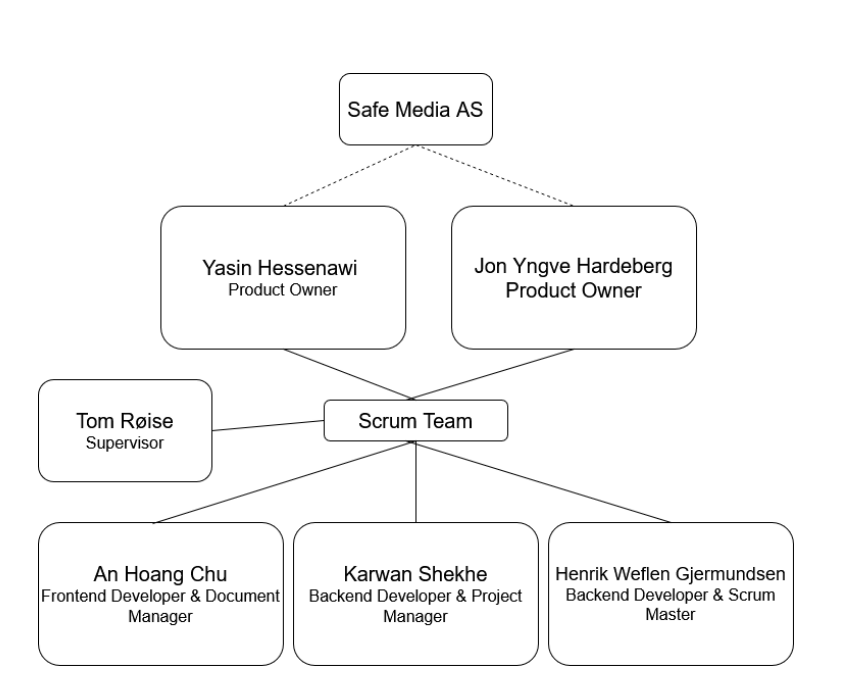
\includegraphics[width=0.85\textwidth]{appendices/scrum_team.png}
    \caption{Scrum team}
\end{figure}

\subsection{Routines and Group Rules}

The complete set of group rules is included in Appendix A. Some key points are outlined below:

\begin{itemize}
    \item Working hours shall be logged, and each member may additionally describe the tasks completed during the week if desired.
    \item These logs are reviewed during project meetings to provide and receive feedback, allowing the group to discuss the work performed by each member.
    \item The group conducts daily Scrum meetings from Monday to Wednesday.
    \item The group holds a meeting with the supervisor every Monday and meets with the project provider every Thursday.
    \item Meeting minutes shall be written after all meetings.
    \item Each group member is expected to allocate several hours after meetings to work together physically at the same location.
    \item Group members shall use the kanban board to assign and prioritize tasks.
    \item Online communication shall take place via Discord.
\end{itemize}

\section{Planning, Follow-up and Reporting}

\subsection{Main breakdown of the project}
\label{appsec:pfar}

We have chosen to use the agile methodology Scrum together with a Kanban board, also called Scrumban. The reason we chose this model is that, in a project like ours, a number of technical uncertainties can arise along the way, which this type of model is well suited for. Another reason is that almost every organization practices agile methods, and the agile Kanban has seen increased popularity especially in software development. Scrum and Kanban are considered as the two powerful Agile methods that handle and manage the progress of software development (Alaidaros \& Omar, 2017; Lei et al., 2017). With a Kanban board we can set up and get an overview of new tasks that appear during the process, and we get a good visualization of workflow and priorities. At the same time, Scrumban allows us to organize the work into short sprints where we can divide the work into phases based on where we are in the project. This methodology also gives us a way of working where it is easy to get feedback from each other/the supervisor/product owner, implement changes continuously, and maintain a good overview.

The way we follow Scrumban in practice is by using Jira as our management tool. In Jira we create issues that we can organize through the columns ``to do'', ``in progress'', ``to test'', ``in review'', ``done''. This is done so that we can visualize the workflow and identify bottlenecks, so tasks do not pile up. This sprint backlog can be updated in connection with the daily scrum, so that we remain flexible during the sprint. Code changes are done via merge requests in GitHub and quality-assured by the rest of the group before it goes into the main branch (see 5.1). An issue is considered finished when it has been confirmed as implemented by everyone in the group and documented to the necessary degree, so that everyone stays aligned on what has been done in the code and can take it into account in meetings.

We will also follow a Gantt chart during the project period. The idea is that we will get an early view of what the whole process will look like from start to finish and be aligned and in agreement on how we will work. The Gantt chart will not be very detailed, but will function as a general breakdown. This is so that we can run Scrumban and still be flexible with tasks, and set short deadlines for ourselves along the way. The Gantt chart is built around longer epics that lead up to a number of milestones and takes decision points into account. We do this so that we can break epics into smaller sprints and have enough time to work and plan/come up with more specific tasks within each epic.

\subsection{Plan for status meetings and decision points during the period}
\label{appsec:}

The plan for the period is to have 1-week sprints at the start and a fixed meeting structure based on that. This is to ensure coordination among the group members so that we can handle challenges and agree on priorities at all times. After that, we will increase the sprint length to 2 weeks or more as needed, again so that we are ready to be flexible:

As a main rule, we will have daily scrum 3--4 times per week, with the purpose of synchronizing progress with each group member. Then we learn what has been done recently and what will be done until the next meeting. We have a meeting lead, and we ensure that all members report their progress status, and we adjust the Kanban board if necessary.

\begin{itemize}
    \item We will have sprint planning at the start of each 2-week sprint. In this meeting we will plan what the sprint goal will be and select issues accordingly.
    \item We will have a sprint review every monday with the supervisor. This is so that we get a good summary of the sprint deliveries, while also receiving feedback we can use later.
    \item After the sprint review we will have a sprint retrospective where we evaluate what worked well during the sprint and what should be improved, as well as actions for the upcoming sprint.
    \item We will also have meetings with the product owner every thursday and meetings with supervisor/other external contacts as needed. All meetings will be documented through shared meeting minutes for logging, and so that we can look back during the process and stay updated on what we have discussed and agreed on.
    \item We will have decision points along the way, which are goals we intend to keep in mind when planning sprints. These are:
    \begin{itemize}
        \item \textbf{Decision point 1: Approval of the project plan.} First of all, we must have good dialogue with the supervisor and agree on a good project plan before we begin the actual task.
        \item \textbf{Decision point 2: Choice of technology/method/model for the final solution.} When we have a plan for how the project will be carried out, we must have a plan for how we will implement the actual solution to the task.
        \item \textbf{Decision point 3: Prototype.} First we must create a working prototype before we can think about adding more functionality/fine-tuning.
        \item \textbf{Decision point 4: Final idea of what will be a feasible plan.} During the project we gain insight into what will be possible to achieve with the task. Here we form an idea of what the final product should ultimately look like.
        \item \textbf{Decision point 5: Feature freeze (no more new functionality).} At some point we will stop implementing and instead focus on polishing/making already implemented functionality work well.
        \item \textbf{Decision point 6: Final demo/delivery.} Finally, we will finalize the product, the report and the full delivery.
    \end{itemize}
\end{itemize}

\section{Organization and Quality Assurance}

\subsection{Documentation, Standards, and Tools}

To ensure a consistent and professional execution of the project, established workflows and best practices are followed. This applies to documentation structure, naming conventions, and coordinated collaboration within the development process. Standardized practices contribute to improved teamwork and easier maintenance.

\subsubsection{Documentation}

Great emphasis is placed on systematic and continuous documentation throughout the entire project. All changes and decisions are documented continuously and regularly to ensure a shared and up-to-date overview of the project's progress.

The group uses a dedicated Discord server as the main platform for internal communication and documentation. Weekly updates and project-related changes are recorded. Henrik, who is responsible as the minute-taker, will write and upload the meeting minutes after each meeting. The meeting minutes include the agenda, meeting objectives, decisions made, and any changes along with their justifications.

\subsubsection{Source Code}

The source code is structured in a clear and organized manner and is commented where necessary to ensure good readability and understanding. This contributes to making the system easier to maintain and extend. In addition, consideration is given to the possibility that the code may be further developed or used by others, and therefore a clear structure and explanatory comments are prioritized.

\subsubsection{Tools}

All source code is stored and version-controlled on GitHub using Git. Changes are documented through commit messages and merge requests with clear titles and short, precise descriptions of the implemented changes.

The frontend is developed using React to enable integration with the client's existing frontend solutions. React is also a well-established and effective framework for developing user interfaces. The backend is developed in Python due to the extensive range of libraries that support machine learning. In addition, Google Cloud is used for running and testing the solution, primarily based on the client's preferences and existing infrastructure.

\begin{longtable}{p{0.14\textwidth}p{0.20\textwidth}p{0.23\textwidth}p{0.33\textwidth}}
\caption{Overview of Tools Used}\\
\toprule
\textbf{Name} & \textbf{Type} & \textbf{Usage Area} & \textbf{Justification} \\
\midrule
\endfirsthead
\toprule
\textbf{Name} & \textbf{Type} & \textbf{Usage Area} & \textbf{Justification} \\
\midrule
\endhead
React & Frontend framework & User interface & Integrates with the client's existing frontend solution \\
Python & Programming language & Backend / AI & Extensive library support for machine learning \\
Google Cloud & Cloud platform & Execution and testing & Preferred platform of the client \\
GitHub & Version control & Source code & Collaboration, traceability, and version control \\
Vite & Build tool & Frontend & Used for fast development and building of the React application \\
Jira & Project management tool & Planning and tracking & Used for task management, progress tracking, and project overview \\
Overleaf & Documentation tool & Report and project plan & Used for collaborative LaTeX documentation \\
Discord & Communication tool & Internal communication & Used for daily communication, meetings, and logging \\
Postman & API tool & Backend testing & Used to test and verify API endpoints \\
Visual Studio Code & Code editor & Development & Primary editor for frontend and backend development \\
Jupyter Notebook & Development tool & Model development and testing & Used for experimentation and testing of machine learning models \\
Figma & Design tool & UI/UX design & Used to sketch and plan user interfaces \\
draw.io & Diagram tool & Architecture and flow & Used to create diagrams and system sketches \\
Docker & Container platform & Deployment and execution & Used to package and run the application consistently \\
\bottomrule
\end{longtable}

\subsubsection{Workflow and Version Control}

To ensure traceability and structure, fixed rules for commit messages are followed. Commit messages are named according to the pattern \texttt{<repository-name>\#<issue-number>}, allowing each change to be directly linked to a specific task or issue in the project. The project follows a structured branching strategy in which the main branch (\texttt{main}) contains only stable and finalized code. All development is carried out through a dedicated development branch (\texttt{dev}). Each group member creates individual feature branches based on \texttt{dev}, tailored to the tasks they are working on, in order to avoid conflicts and ensure controlled code integration.

Working branches are named according to the pattern:

\begin{quote}
\texttt{<name>/<branch-prefix>/<short-description>}.
\end{quote}

Branch prefixes are used to clearly indicate the purpose of the change. The following prefixes are used in the project:

\begin{itemize}
    \item \texttt{feat/} -- new functionality
    \item \texttt{fix/} -- bug fixes
    \item \texttt{docs/} -- documentation
    \item \texttt{test/} -- tests
    \item \texttt{refactor/} -- code restructuring without changing functionality
\end{itemize}

This structure contributes to good overview, reduces the risk of conflicts within the codebase, and facilitates safe and controlled development.

\subsection{Inspection and Testing Plan}

Throughout the project development, thorough testing is essential. Testing is used to ensure correct functionality and quality both during and after the development phase. The project places emphasis on unit, integration, and system testing.

\begin{itemize}
    \item \textbf{Unit testing (automated):} Focuses on testing individual components, methods, and functions of the source code in isolation.
    \item \textbf{API testing (automated or manual):} Validates API endpoints to ensure they function as expected and meet performance requirements.
    \item \textbf{Integration testing (automated or manual):} Verifies that different modules or services work correctly when combined.
    \item \textbf{System testing:} Evaluates the fully integrated system as a whole to ensure that all requirements are met.
    \item \textbf{User testing:} Users and the client are involved in evaluating the system to identify potential improvements.
\end{itemize}

Implemented functionality is tested immediately after implementation by verifying expected behavior and addressing any detected issues. Testing helps identify errors early and ensures the stability and reliability of the solution.

\subsection{Project-Level Risk Analysis}

A project-level risk analysis has been conducted to identify potential events that may affect the project's execution, progress, and collaboration within the group.

The risks are assessed based on probability and impact and are placed in a risk matrix, as shown in Table~\ref{tab:project-plan-risk-matrix}. Based on this assessment, specific risk factors have been identified and are presented in Table~\ref{tab:project-plan-identified-risks}, where both probability and impact are indicated.

To keep the analysis focused and relevant, risks with low probability and low impact have been excluded from the mitigation table, as they are considered manageable through normal project routines. The mitigation measures present in Table~\ref{tab:project-plan-risk-mitigation} therefore focus on the most significant risks.

For each identified risk, risk mitigation measures have been defined to prevent, reduce, or manage the consequences should the risk occur. These measures are summarized in Table~\ref{tab:project-plan-risk-mitigation}. The risk analysis will be updated as needed throughout the project period.

\begin{table}[H]
\centering
\caption{Risk Matrix (5x5)}
\label{tab:project-plan-risk-matrix}
\begin{tabular}{lccccc}
\toprule
\textbf{Probability / Impact} & \textbf{Minimal} & \textbf{Marginal} & \textbf{Moderate} & \textbf{Severe} & \textbf{Critical} \\
\midrule
Almost Certain & & & & & \\
Likely & & & & & \\
Possible & & & & & \\
Unlikely & & & & & \\
Rare & & & & & \\
\bottomrule
\end{tabular}
\end{table}

\begin{longtable}{p{0.08\textwidth}p{0.60\textwidth}p{0.14\textwidth}p{0.12\textwidth}}
\caption{Identified Risks}\label{tab:project-plan-identified-risks}\\
\toprule
\textbf{Risk \#} & \textbf{Description} & \textbf{Probability} & \textbf{Impact} \\
\midrule
\endfirsthead
\toprule
\textbf{Risk \#} & \textbf{Description} & \textbf{Probability} & \textbf{Impact} \\
\midrule
\endhead
1 & Technical challenges related to the use of new technology. & Possible & Moderate \\
2 & Loss or corruption of source code and documentation. & Possible & Critical \\
3 & Insufficient or delayed communication with the client. & Unlikely & Severe \\
4 & Risk of reduced backend performance due to the use of Python and machine learning libraries. & Possible & Moderate \\
5 & The AI model misclassifies sensitive information (false negatives and false positives), resulting in either missed anonymization of sensitive content or unnecessary anonymization of non-sensitive content. & Possible & Critical \\
6 & Errors or performance issues are detected late in the testing phase, leading to delays or reduced solution quality. & Likely & Severe \\
7 & User testing reveals significant usability issues that require changes to design or functionality. & Likely & Severe \\
8 & Lack of communication in the group & Unlikely & Severe \\
9 & Delays in the project due to time consumptions and coordinations. & Unlikely & Moderate \\
10 & Uneven workload distribution within the group. & Unlikely & Moderate \\
11 & Illness or absence of one or more group members. & Unlikely & Minimal \\
\bottomrule
\end{longtable}

\begin{longtable}{p{0.08\textwidth}p{0.70\textwidth}p{0.14\textwidth}}
\caption{Risk Mitigation Measures}\label{tab:project-plan-risk-mitigation}\\
\toprule
\textbf{Risk \#} & \textbf{Mitigation Measures} & \textbf{Priority} \\
\midrule
\endfirsthead
\toprule
\textbf{Risk \#} & \textbf{Mitigation Measures} & \textbf{Priority} \\
\midrule
\endhead
1 & Early prototyping and close dialogue with the supervisor and client to reduce technical uncertainty. & Medium \\
2 & Use cloud-based storage services and perform regular backups. & High \\
3 & Ensure clear communication channels and fixed points of contact with the client and supervisor. & Medium \\
4 & Limit scope, use efficient models, and test performance early. & Medium \\
5, 6 & Use well-documented models, conduct thorough testing, and combine automated and manual evaluation of results. & High \\
7 & Test functionality and performance early and continuously throughout the development process. & High \\
8 & Involve users and the client early in the testing phase and iterate on the solution based on feedback. & High \\
\bottomrule
\end{longtable}

\section{Plan for Implementation}

\subsection{Progress-plan (Gantt-chart)}

\begin{figure}[H]
    \centering
    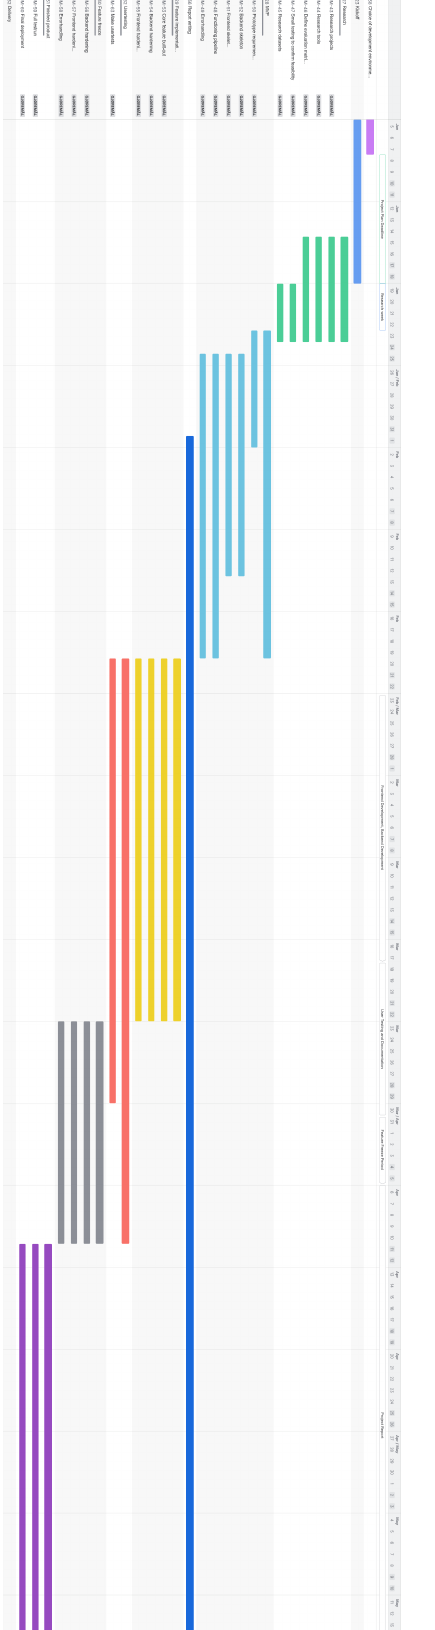
\includegraphics[height=0.75\textheight,keepaspectratio]{appendices/gantt_chart.png}
    \caption{Gantt chart for the project timeline.}
\end{figure}

\subsection{Milestones and Decision Points}

\begin{itemize}
    \item \textbf{Milestone 1, Choice of Development Environment (January 5 - January 7).} Decide between GitLab or GitHub, set up a Kanban board, assign roles, and handle other administrative tasks.
    \item \textbf{Milestone 2, Preliminary Project Deadline (January 8 - January 18).} Sign the group contract and complete the project plan.
    \item \textbf{Milestone 3, Research and Data Collection (January 15 - January 23).} Conduct research on similar projects and identify models that can be used for this project.
    \item \textbf{Milestone 4, Frontend and Backend prototype with destroy philosphy (January 23 - February 1.).} Test all tools for frontend and backend. Do work, but be ready to scrap and destroy progress that didnt work. Then we start over again and work on the real MVP with the gained experience.
    \item \textbf{Milestone 5, Frontend and Backend development (MVP) (January 23 - February 12).} Start frontend development and establish a pipeline for the backend.
    \item \textbf{Milestone 6, Backend Integration with Frontend (MVP) (February 12 - February 19).} Develop the backend and integrate it with the frontend.
    \item \textbf{Milestone 7, Feature implementations (February 19 - March 22).} Develop features to both frontend and backend/harden functionality.
    \item \textbf{Milestone 8, Project Testing, Documentation (February 20 - April 10).} Conduct user tests, double-check all existing tests and ensure documentation is complete where needed.
    \item \textbf{Milestone 9, Development Deadline (March 23 - April 10).} Feature freeze: no new additions, only refining existing work. Make the product as strong and reliable as possible with no more added features. Incorporate feedback from user tests and prepare everything for final submission.
    \item \textbf{Milestone 10, Project Report Writing (February 1 - May 16).} Begin writing the report and aim to complete it.
    \item \textbf{Milestone 11, Bachelor Project Deadline (May 16 - May 20).} Double-check that everything is ready for submission and polish the report.
\end{itemize}

\section{Gruppe kontrakt}

\begin{center}
    \Large\textbf{Gruppe konrakt - IDATG2901}\\[0.5em]
    An Hoang Chu, Henrik Weflen Gjermundsen, Karwan Shekhe\\[0.5em]
    Januar 2026
\end{center}

\subsection{Kontraktoverskrift}

Kontrakten gjelder for disse medlemmene:

\begin{itemize}
    \item An Hoang Chu
    \item Henrik Weflen Gjermundsen
    \item Karwan Shekhe
\end{itemize}

Kontrakten er gylding til 06.06.2026.

\subsection{Kommunikasjon og diskusjon}

\begin{itemize}
    \item Medlemmene skal kommunisere og diskutere sammen gjennom hele prosjektet, både fysisk og digitalt. Dersom noen blir syke eller er borte over lengre tid, skal dette kommuniseres tydelig, da det er viktig informasjon for resten av gruppen.
    \item Oppgave fordelig blir bestem gjennom diskusjon sammen blant gruppen, og blir tildelt på Jira sitt kanban. Denne diskusjonen bør skje under møtene og sprints. I tillegg blir det kommunisert på hvem som har kodet hva gjennom GitHub.
    \item Dersom det blir vanskelig å komme seg til en beslutning felles vil det være prosjektlederen som tar det endelige valget for gruppen.
\end{itemize}

\subsection{Ansvar og roller}

Rollene blir fordelt blant medlemmene etter at de har diskutert hvem de mener er egnet best for hva. Disse tre rollene blir prosjekt ansvarlig, scrum master og en dokument ansvarlig. Selv om det blir delt tre forskjellige roller innad gruppen, er enda alle tre utviklere.

\begin{itemize}
    \item Prosjekt ansvarlig tar ansvar for innholdet i prosjektet og hvordan det skal utføres. Passer også på at prosjektet går riktig vei og at kriterier blir møtt på god tid. Sørger for at det som blir pusha inn til Git er korrekt og holder øye på merges.
    \item Scrum master sørger for at møtereferater blir skrevet under hvert møte og setter opp møter og sprints. Holder øyet på at møtene ikke kræsjer med resten av medlemmene sine timeplaner og får møte i gang.
    \item Dokument ansvarlig passer på at dokumeneter er klare før fristende og at de er innafor kriteriene. Sørger for at alle formelle krav er oppfylt og dobbelsjekker kildene som brukes. Får alle medlemmer til å lese gjennom dokumentene slik at alle er enig om det som står der.
\end{itemize}

\subsection{Regler}

Under prosjekt perioden av gruppe kontrakten vil det være noen regler som bør bli holdt for å ha gode rutiner og bra arbeidsmoral.

\begin{itemize}
    \item Gruppe medlemmene skal samarbeide aktivt gjennom hele prosessen og dele kunnskap og ressurser innad gruppen.
    \item Oppgaver som blir tildelt må bli gjort og hver medlem bør ta iniativ til å gi seg selv flere oppgaver dersom de blir ferdig med sine opprinnelige oppgaver.
    \item Ikke lov til å gi seg selv flere enn tre issues.
    \item Reviews bør prioriteres, helst fullføre reviews før man går videre med sine issues.
    \item Det er obligatorisk å hjelpe en annen medlem når de spør om hjelp og sitter fast på noe.
    \item Alle skal passe på at de er oppdatert med arbeidet gjennom Jira og GitHub.
    \item Gruppe medlemmer er klare og vet når og hvor møtene skal holdes.
    \item Det skal være minst 30 timer med arbeid hver uke.
    \item Timer skal bli loggført.
\end{itemize}

\subsection{Møter}

Det vil være et første møte hvor gruppe medlemmer diskuterer innholdet i gruppe kontrakten og signerer det, samtidig fordeler roller og diskuterer fremtiden for gruppen. Det vil bli holdt daily scrums fra tirsdag til torsdag, hvor møtet på torsdag blir med oppdragsgiverene våres. I tillegg har vi en sprint review og retrospektiv hver mandag etter møtet med veileder. Møtene skal være fysisk på campus, men hvis to av tre medlemmer er syke kan det arrangeres en annen tid, dette bør kommuniseres på god tid.

Ved å signere dette dokumentet godtar du punktene over.

\vspace{2em}
\textbf{Signert av:}

\vspace{3em}
\begin{tabular}{p{0.3\textwidth}p{0.3\textwidth}p{0.3\textwidth}}
An Hoang Chu & Henrik Weflen Gjermundsen & Karwan Shekhe \\
\end{tabular}

\endgroup

% Full project hour tracking appendix generated from TimelisteBachelor2026.xlsx
% Recommended packages in the preamble:
% \usepackage{booktabs}
% \usepackage{longtable}
% \usepackage{array}
% \usepackage{graphicx}
% \usepackage{float}

\chapter{Project Hour Tracking}
\label{app:project-hour-tracking}
\raggedbottom

This appendix presents the project hour tracking maintained throughout the bachelor project. The hour list was used to document weekly work distribution across planning, meetings, documentation, programming, testing, research, figures, and administration. The appendix first presents a condensed overview of the total work distribution, followed by the complete weekly hour logs from the original spreadsheet.

\section{Condensed Overview}
\label{appendix:project-hour-tracking-overview}

\begin{table}[htbp]
\centering
\caption{Total registered project hours by group member.}
\label{tab:project-hours-member-total}
\begin{tabular}{lr}
\toprule
Group member & Total hours \\
\midrule
Hoang & 723 \\
Henrik & 674 \\
Karwan & 788.5 \\
\midrule
Total & 2185.5 \\
\bottomrule
\end{tabular}
\end{table}

\begin{table}[htbp]
\centering
\caption{Total registered project hours by activity category.}
\label{tab:project-hours-category-total}
\begin{tabular}{lr}
\toprule
Activity category & Total hours \\
\midrule
Programming & 729 \\
Report documentation & 579 \\
Planning and meetings & 309 \\
Research & 254 \\
Testing & 104 \\
Git and administration & 103.5 \\
Figures and diagrams & 63.5 \\
Code documentation & 43.5 \\
\midrule
Total & 2185.5 \\
\bottomrule
\end{tabular}
\end{table}

\begin{figure}[htbp]
    \centering
    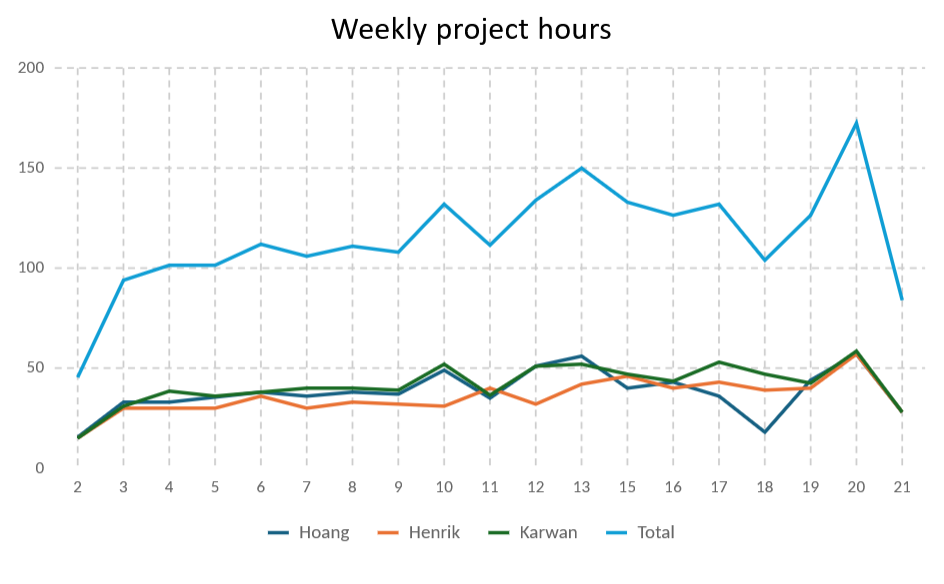
\includegraphics[width=0.85\textwidth]{figures/images/chapter-3/project_hours_weekly_summary_user_chart.png}
    \caption{Summary of registered project hours across the project period.}
    \label{fig:project-hours-weekly-summary}
\end{figure}

\begin{figure}[htbp]
    \centering
    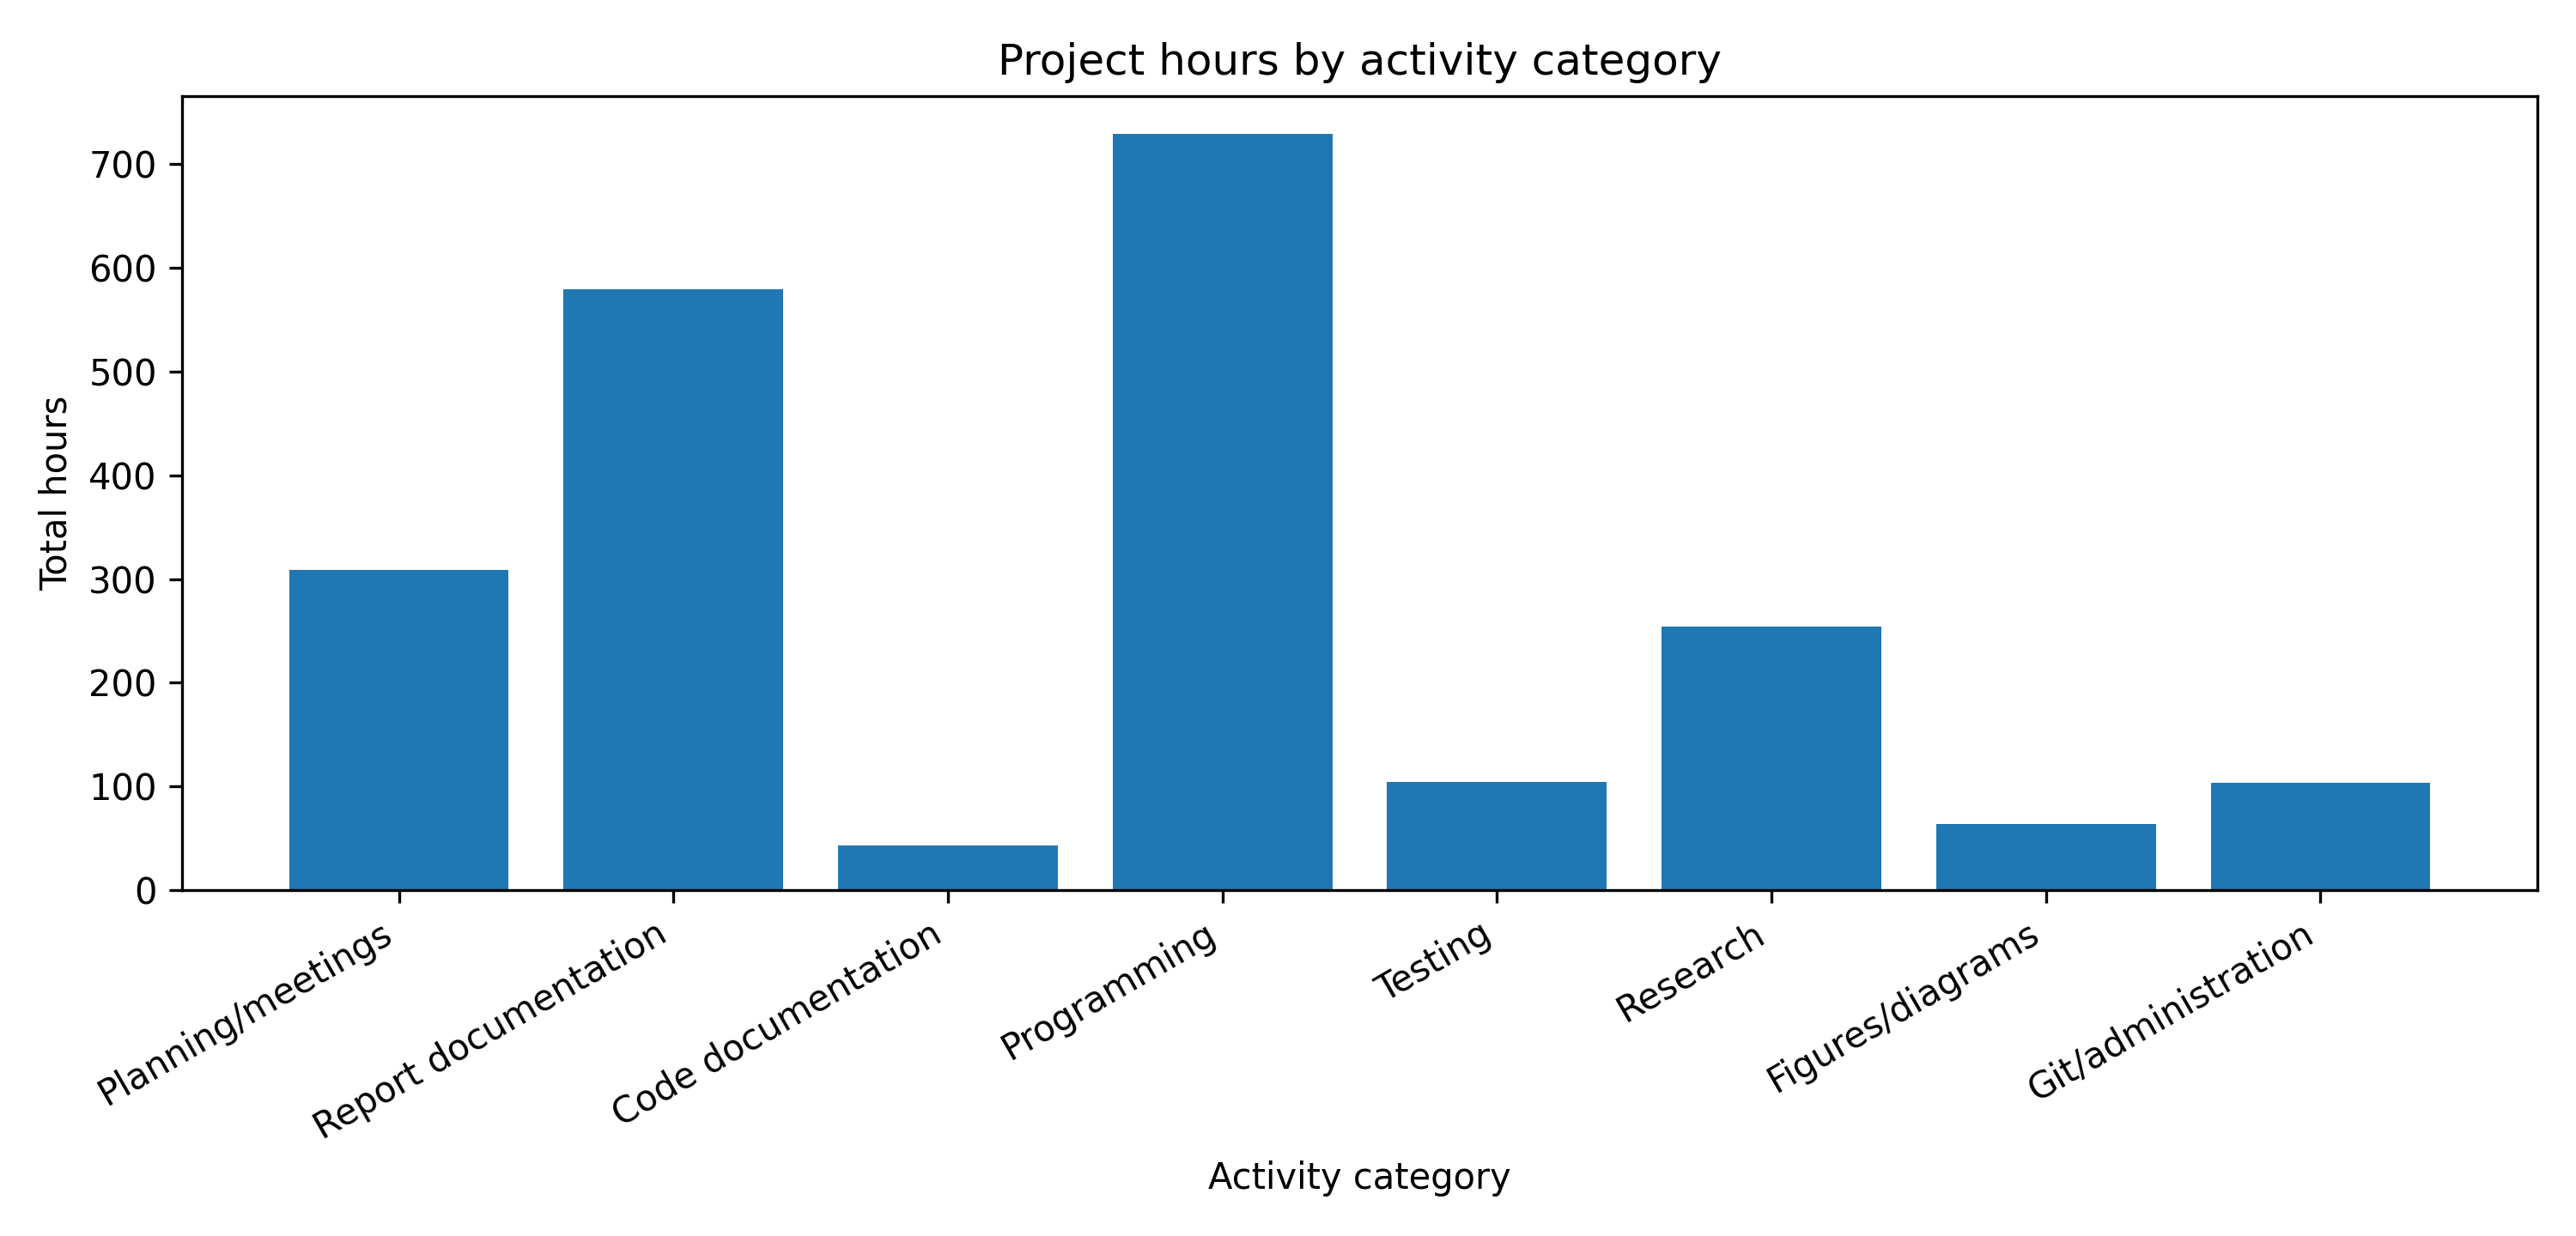
\includegraphics[width=0.80\textwidth]{figures/images/chapter-3/project_hours_category_summary.png}
    \caption{Distribution of registered project hours by activity category.}
    \label{fig:project-hours-category-summary}
\end{figure}

\begin{longtable}{lrrrr}
\caption{Weekly registered project hours by group member.}
\label{tab:project-hours-weekly-overview}\\
\toprule
Week & Hoang & Henrik & Karwan & Total \\
\midrule
\endfirsthead
\toprule
Week & Hoang & Henrik & Karwan & Total \\
\midrule
\endhead
Uke2 & 15.5 & 15 & 15 & 45.5 \\
Uke3 & 33 & 30 & 31 & 94 \\
Uke4 & 33 & 30 & 38.5 & 101.5 \\
Uke5 & 35.5 & 30 & 36 & 101.5 \\
Uke6 & 38 & 36 & 38 & 112 \\
Uke7 & 36 & 30 & 40 & 106 \\
Uke8 & 38 & 33 & 40 & 111 \\
Uke9 & 37 & 32 & 39 & 108 \\
Uke10 & 49 & 31 & 52 & 132 \\
Uke11 & 35 & 40 & 36.5 & 111.5 \\
Uke12 & 51 & 32 & 51 & 134 \\
Uke13 & 56 & 42 & 52 & 150 \\
Uke15 & 40 & 46 & 47 & 133 \\
Uke16 & 43 & 40 & 43.5 & 126.5 \\
Uke17 & 36 & 43 & 53 & 132 \\
Uke18 & 18 & 39 & 47 & 104 \\
Uke19 & 44 & 40 & 42.5 & 126.5 \\
Uke20 & 57 & 57 & 58.5 & 172.5 \\
Uke21 & 28 & 28 & 28 & 84 \\
\midrule
Total & 723 & 674 & 788.5 & 2185.5 \\
\bottomrule
\end{longtable}

\section{Complete Weekly Hour Logs}
\label{appendix:project-hour-tracking-complete}

The following tables reproduce the complete weekly hour logs from the project hour list. Each week includes the registered hours by activity category and group member. When the spreadsheet included written comments, these are included below the corresponding weekly hour table.

\subsection{Uke2}

\begin{table}[H]
\centering
\small
\caption{Registered hours for Uke2.}
\label{tab:project-hours-uke2}
\begin{tabular}{lrrrr}
\toprule
Activity & Hoang & Henrik & Karwan & Total \\
\midrule
Møter & 4 & 4 & 4 & 12 \\
Dokumentasjon - Rapport & 5 & 6 & 5 & 16 \\
Dokumentasjon - Kode & 0 & 0 & 0 & 0 \\
Programmering & 0 & 0 & 0 & 0 \\
Testing & 0 & 0 & 0 & 0 \\
Forskning & 4 & 2 & 3 & 9 \\
Figurer og diagrammer & 0.5 & 1.5 & 1 & 3 \\
Git / Administrasjon & 2 & 1.5 & 2 & 5.5 \\
\midrule
Total & 15.5 & 15 & 15 & 45.5 \\
\bottomrule
\end{tabular}
\end{table}

\begin{longtable}{p{0.20\textwidth}p{0.72\textwidth}}
\caption{Written activity notes for Uke2.}\\
\toprule
Entry & Notes \\
\midrule
\endfirsthead
\toprule
Entry & Notes \\
\midrule
\endhead
Hoang & Satte opp GitLab Kanban tavle og excel dokumentet. \newline Tok kontakt med OsloSkolen for mulig samarbeid. \newline Satte opp gruppe kontrakt og fikk signaturer. \newline Ansvar for kapittel en og tre for prosjektplanen. \\
\addlinespace
Henrik & Har skrevet punkt 4 om planlegging, oppfølging og rapportering. Har skrevet møtereferater og satt opp online møter. Har laget kanaler hvor vi kan snakke sammen og dele felles dokumenter/organisere ting vi har diskutert etter tema slik at vi lett kan finne fram og være oppdatert. Har utforsket teori om oppgaven. \\
\addlinespace
Karwan & Forskning: Forbredelse ved å lese tidligere bachleor oppgaver. Møter: Henvend til møtereferatene fra uke 2. Rapportering: Skrive "Organisering og Kvalitetssikring" og analysere risiko. Kontakte ulike bedrifter for mulige bachleor oppgaver. \\
\addlinespace
\bottomrule
\end{longtable}

\subsection{Uke3}

\begin{table}[H]
\centering
\small
\caption{Registered hours for Uke3.}
\label{tab:project-hours-uke3}
\begin{tabular}{lrrrr}
\toprule
Activity & Hoang & Henrik & Karwan & Total \\
\midrule
Møter & 7 & 8 & 7 & 22 \\
Dokumentasjon - Rapport & 9 & 6 & 7 & 22 \\
Dokumentasjon - Kode & 0 & 0 & 0 & 0 \\
Programmering & 0 & 0 & 0 & 0 \\
Testing & 0 & 0 & 0 & 0 \\
Forskning & 10 & 6 & 14 & 30 \\
Figurer og diagrammer & 1 & 6 & 2 & 9 \\
Git / Administrasjon & 6 & 4 & 1 & 11 \\
\midrule
Total & 33 & 30 & 31 & 94 \\
\bottomrule
\end{tabular}
\end{table}

\begin{longtable}{p{0.20\textwidth}p{0.72\textwidth}}
\caption{Written activity notes for Uke3.}\\
\toprule
Entry & Notes \\
\midrule
\endfirsthead
\toprule
Entry & Notes \\
\midrule
\endhead
Hoang & Bearbeidet prosjektplanen, og har sett på en del research angående sladding av sensitiv informasjon på bilder, hvordan andre modeller har gjort det kontra våres potensiell løsnign. Har også gjort en del research om react rammeverket og hvordan det brukes for å lage nettsider, I tillegg til å eksperimentere med rammeverket. Har også satt opp GitHub og Jira, og vurdert hvilken kanban tavle som er best (kollektivt). Opprettet frontend prosjektet og initialisert til GitHub. \\
\addlinespace
Henrik & Jobbet videre med prosjektplanen. Skrevet møtereferater og notert på møter. Oppsummert møter og vært scrum ansvarlig. Kommet på ideer til løsninger. Bidrat til spørsmål til oppdragsgiver/rådgiver. Laget Gantt skjema og kommet på plan for prosjektets tidslinje. Hjulpet med å komme på løsning til administrasjon og sette opp Jira. \\
\addlinespace
Karwan & Bruke tid på å se etter eksisterende løsninger innen ansiktdjenskjenning og ansiktsdetection. Se etter modeller som kan brukes i prosjektet. Lese teori innen maskin læring. Teste disse ulike eksisterende løsningene på python og se om det er noe å ta med. Pusse opp omfang delen i prosjekt rapporten. Fikse Wiki page for GitHub. \\
\addlinespace
\bottomrule
\end{longtable}

\subsection{Uke4}

\begin{table}[H]
\centering
\small
\caption{Registered hours for Uke4.}
\label{tab:project-hours-uke4}
\begin{tabular}{lrrrr}
\toprule
Activity & Hoang & Henrik & Karwan & Total \\
\midrule
Møter & 7 & 8 & 7 & 22 \\
Dokumentasjon - Rapport & 4 & 5 & 4 & 13 \\
Dokumentasjon - Kode & 0 & 0 & 1 & 1 \\
Programmering & 17 & 0 & 20 & 37 \\
Testing & 0 & 0 & 2 & 2 \\
Forskning & 3 & 10 & 4 & 17 \\
Figurer og diagrammer & 0 & 2 & 0.5 & 2.5 \\
Git / Administrasjon & 2 & 5 & 0 & 7 \\
\midrule
Total & 33 & 30 & 38.5 & 101.5 \\
\bottomrule
\end{tabular}
\end{table}

\begin{longtable}{p{0.20\textwidth}p{0.72\textwidth}}
\caption{Written activity notes for Uke4.}\\
\toprule
Entry & Notes \\
\midrule
\endfirsthead
\toprule
Entry & Notes \\
\midrule
\endhead
Hoang & Brukt meste av tiden til å utvikle en prototype som skal bli kastet på react + vite i tillegg til litt research om best practices innen for dem. Fått til en enkel nettside med enkel redigering. Redigert litt på prosjektplanen etter tilbakemelding fra veileder og passe på at språket er mer konsistent. \\
\addlinespace
Henrik & Ferdigstillte prosjektrapport. Fant state of the art av image preprocessing for facedetection, object detection og character detection. Researchet hva som menes med sensitiv informasjon/hva som brukes i praksis. Skrev møtereferater, passet på at scrum ble fulgt. \\
\addlinespace
Karwan & Research innen face recognition og face detection. Finne modeller som gir gode resultater. Testing for å gjøre disse modellene bedre. Vi valgte RetinaFace for å finne ansikter i bilder, for den er den største modellen og som gir veldig gode resultater, både av små ansikter (distanse ) og gruppe bilder. Retina er dårlig på å finne ansikter som ikke vises fult (f.eks hjelm, maske, osv), la til augmentasjion + occulation for å gjøre modellen bedre. Bruker YOLO for å finne fulle kropper og ikke bare ansikter. Evaluere modellene, sammenligne fine tuned modell med base modellen. \\
\addlinespace
\bottomrule
\end{longtable}

\subsection{Uke5}

\begin{table}[H]
\centering
\small
\caption{Registered hours for Uke5.}
\label{tab:project-hours-uke5}
\begin{tabular}{lrrrr}
\toprule
Activity & Hoang & Henrik & Karwan & Total \\
\midrule
Møter & 5 & 6 & 5 & 16 \\
Dokumentasjon - Rapport & 4 & 1 & 1 & 6 \\
Dokumentasjon - Kode & 3 & 0 & 1 & 4 \\
Programmering - Front & 18 & 0 & 0 & 18 \\
Programmering - Back & 0 & 7 & 19 & 26 \\
Testing & 1 & 1 & 1 & 3 \\
Forskning & 2 & 13 & 8 & 23 \\
Figurer og diagrammer & 0.5 & 1 & 0 & 1.5 \\
Git / Administrasjon & 2 & 1 & 1 & 4 \\
\midrule
Total & 35.5 & 30 & 36 & 101.5 \\
\bottomrule
\end{tabular}
\end{table}

\begin{longtable}{p{0.20\textwidth}p{0.72\textwidth}}
\caption{Written activity notes for Uke5.}\\
\toprule
Entry & Notes \\
\midrule
\endfirsthead
\toprule
Entry & Notes \\
\midrule
\endhead
Hoang & Skrev siste endringer (GDPR og regler) på prosjektplan etter møte med oppdragsgiver, samtidig som tankekartet ble revidert. La til manuell sladding i frontend samtidig enkle funksjonalitet som å laste ned filen og zoome in og ut på bildet. Protoypen ble refaktorert og satt inn i MVP repo. Dokumentasjon for klassene ble lagt til, kompleks logikk fikk kommentarer. Sett bittelitt på hvordan GitHub Actions fungerer og satt det opp. \\
\addlinespace
Henrik & Researchet/laget og testet kode for preprocessing av bilder opp mot retinaface-modellen. Hvilke threshholds/hva slags preprocessing gjør at modellen klarer å finne flest ansikter i en folkemengde. Hva fungerer best på bilder med forskjellig stø. Hva vil være beste metode med tanke på tid modellen bruker. Dersom vi skal legge til tekst i framtiden, hva slags preprocessing gjøres for å detektere områder der tekst mest sannsynlig ligger i bildet. Skrevet på rapport. Endret på Gannt skjema. \\
\addlinespace
Karwan & Finpusse prosjektplan rapporten. Gå gjennom for å bekrefte den før levering. Implementere pipeline for backend slik at den kan senere bli brukt av frontend. Implementere API, og ulike endepunkter for å sende informasjon. Fine-tune retinaface modellen for å se om vi kan gjøre den bedre enn base modellen. \\
\addlinespace
\bottomrule
\end{longtable}

\subsection{Uke6}

\begin{table}[H]
\centering
\small
\caption{Registered hours for Uke6.}
\label{tab:project-hours-uke6}
\begin{tabular}{lrrrr}
\toprule
Activity & Hoang & Henrik & Karwan & Total \\
\midrule
Oppgave Tema & 0 & 0 & 0 & 0 \\
Planlegging/Møter & 5 & 6 & 5 & 16 \\
Dokumentasjon - Rapport & 0 & 6 & 0 & 6 \\
Dokumentasjon - Kode & 3 & 0 & 2 & 5 \\
Programmering - Front & 26 & 0 & 2 & 28 \\
Programmering - Back & 0 & 13 & 25 & 38 \\
Testing & 0 & 0 & 1 & 1 \\
Forskning & 2 & 10 & 2 & 14 \\
Figurer og diagrammer & 0 & 0 & 0 & 0 \\
Git / Administrasjon & 2 & 1 & 1 & 4 \\
\midrule
Total & 38 & 36 & 38 & 112 \\
\bottomrule
\end{tabular}
\end{table}

\begin{longtable}{p{0.20\textwidth}p{0.72\textwidth}}
\caption{Written activity notes for Uke6.}\\
\toprule
Entry & Notes \\
\midrule
\endfirsthead
\toprule
Entry & Notes \\
\midrule
\endhead
Hoang & Riktig skalering på knapper og komponenter avhengig av vindu størrelse er nå implementert. Lagt til andre UI/UX elementer som kan hjelpe bruker opplevelsen. PDF er nå redigerbar. Prøvd å refaktorere koden, men må jobbes mer med. Har satt opp inndeling for prosjekt rapporten. \\
\addlinespace
Henrik & Har jobbet med segmentation av personer i bildene i backend. Har gjort forskning på gdpr, state of the art og så vidt begynt på rapporten for kapittel 2. \\
\addlinespace
Karwan & Optimalisere hastigheten til redaction av ansikter, for redaction var unødvendig treig. Gi mulighet til brukeren slik at de kan velge ut hva slags ansikter de ikke vil redacte. Gjøre anonymisering sterkere. Bruke Go som offisiel språk for API. Rydde og refaktorisere koden slik at det er ryddig, legge til dokumentasjon. \\
\addlinespace
\bottomrule
\end{longtable}

\subsection{Uke7}

\begin{table}[H]
\centering
\small
\caption{Registered hours for Uke7.}
\label{tab:project-hours-uke7}
\begin{tabular}{lrrrr}
\toprule
Activity & Hoang & Henrik & Karwan & Total \\
\midrule
Planlegging/Møter & 5 & 6 & 5 & 16 \\
Dokumentasjon - Rapport & 14 & 8 & 0 & 22 \\
Dokumentasjon - Kode & 0 & 0 & 1 & 1 \\
Programmering - Front & 2 & 0 & 10 & 12 \\
Programmering - Back & 0 & 0 & 12 & 12 \\
Testing & 0 & 0 & 5 & 5 \\
Forskning & 9 & 14 & 5 & 28 \\
Figurer og diagrammer & 2 & 0 & 0 & 2 \\
Git / Administrasjon & 4 & 2 & 2 & 8 \\
\midrule
Total & 36 & 30 & 40 & 106 \\
\bottomrule
\end{tabular}
\end{table}

\begin{longtable}{p{0.20\textwidth}p{0.72\textwidth}}
\caption{Written activity notes for Uke7.}\\
\toprule
Entry & Notes \\
\midrule
\endfirsthead
\toprule
Entry & Notes \\
\midrule
\endhead
Hoang & Inndelte kapitlene enda mer I overleaf for å lage grov oversikt over hva som skal med, basert på tidligere bachelor oppgaver. Startet med første chapter for bachelor oppgavene, altså om oppgavebeskrivelsen, mål, rammer, osv. Gjorde en del research om lignende oppgaver og om modeller som kan brukes for tekst og om lisenser som trengs. I tillegg lest en del bachelor oppgaver for å få helhetelig bildet på hvordan våres skal se ut. \\
\addlinespace
Henrik & Har researchet gdpr, state of art, begynt på rapporten og sett på mulige løsninger for videreutvikling av koden. \\
\addlinespace
Karwan & Refaktorere koden til frontend og backend. Ridde opp dokumentasjoner, dele opp koden. Refaktorere mappe struktur. Fikse bugs, blant annent som synkronisere manuel redaction med automatisk redaction. Gjøre hastigheten til redaction bedre. Legge til CRAFT (tekst deteksjon) til backend og koble den til frontend. Forskning innen ulike modeller for tekstdeteksjon innen bilder. \\
\addlinespace
\bottomrule
\end{longtable}

\subsection{Uke8}

\begin{table}[H]
\centering
\small
\caption{Registered hours for Uke8.}
\label{tab:project-hours-uke8}
\begin{tabular}{lrrrr}
\toprule
Activity & Hoang & Henrik & Karwan & Total \\
\midrule
Planlegging/Møter & 5 & 6 & 5 & 16 \\
Dokumentasjon - Rapport & 6 & 0 & 0 & 6 \\
Dokumentasjon - Kode & 1 & 0 & 1 & 2 \\
Programmering - Front & 14 & 10 & 2 & 26 \\
Programmering - Back & 0 & 8 & 23 & 31 \\
Programmering - Bugs & 5 & 2 & 1 & 8 \\
Testing & 0 & 0 & 3 & 3 \\
Forskning & 4 & 5 & 3 & 12 \\
Figurer og diagrammer & 0 & 0 & 1 & 1 \\
Git / Administrasjon & 3 & 2 & 1 & 6 \\
\midrule
Total & 38 & 33 & 40 & 111 \\
\bottomrule
\end{tabular}
\end{table}

\begin{longtable}{p{0.20\textwidth}p{0.72\textwidth}}
\caption{Written activity notes for Uke8.}\\
\toprule
Entry & Notes \\
\midrule
\endfirsthead
\toprule
Entry & Notes \\
\midrule
\endhead
Hoang & Prøvd å ta litt kontakt med ulike potenseille bruketestere som for eksempel fra NRK eller VG. Brukt tid på å legge til bruke innstillinger I applikasjonen vår, I tillegg til å fikse noen bugs. Har satt opp overleaf dokumentet etter ntnu sine standarder og holder på å overføre tekst fra den gamle. Gjort litt mer forksning på the state of art. \\
\addlinespace
Henrik & Jobbet med downscaling methods i backend. Fikset terms of service i frontend. Lagde to forskjellige brukertester, en tilpasset testing for funksjonalitet og en for UI. \\
\addlinespace
Karwan & Fjerne PDF støtte pga ikke lenger behov, forenkle frontend for kunn bilde støtte. Teste alle ende punkter (redact\&detect) og sørge for at de fungerer. Dekke så mye av backend koden som mulig med unit testing. Legge til script for å starte frontend og backend enkelt samtidig (loklat). Contrainerize backend med docker. Fikse Google Cloud Run for å kunne deploye applikasjonen. Legge til dokumenatison i koden. Evaluere retinaface modelene (resnet50 og mobilnet\_25) for rapport og prøve å fine tune den. \\
\addlinespace
\bottomrule
\end{longtable}

\subsection{Uke9}

\begin{table}[H]
\centering
\small
\caption{Registered hours for Uke9.}
\label{tab:project-hours-uke9}
\begin{tabular}{lrrrr}
\toprule
Activity & Hoang & Henrik & Karwan & Total \\
\midrule
Planlegging/Møter & 5 & 6 & 5 & 16 \\
Dokumentasjon - Rapport & 3 & 0 & 0 & 3 \\
Dokumentasjon - Kode & 1 & 0 & 1 & 2 \\
Programmering - Front & 21 & 0 & 10 & 31 \\
Programmering - Back & 0 & 7 & 15 & 22 \\
Programmering - Bugs & 0 & 0 & 5 & 5 \\
Testing & 2 & 9 & 1 & 12 \\
Forskning & 4 & 4 & 1 & 9 \\
Figurer og diagrammer & 0 & 3 & 0 & 3 \\
Git / Administrasjon & 1 & 3 & 1 & 5 \\
\midrule
Total & 37 & 32 & 39 & 108 \\
\bottomrule
\end{tabular}
\end{table}

\begin{longtable}{p{0.20\textwidth}p{0.72\textwidth}}
\caption{Written activity notes for Uke9.}\\
\toprule
Entry & Notes \\
\midrule
\endfirsthead
\toprule
Entry & Notes \\
\midrule
\endhead
Hoang & La til ulike UI/UX funksjonaliteter som for eksempel farge endring, filtere og brukerpreferanser. Har startet med å legge til noe support for video og videoformatering. Gjort research på hvordan tidligere prosjekter/andre bedrifter og firmaer og gjort denne løsningen. Forbedret biter fra chapter 1 fra det gamle overleaf dokumentet. Har også sett på standarder innen for testing og hvordan testing skal være, i tillegg til å lage nye test filer og oppdatere den gamle test filen. \\
\addlinespace
Henrik & Tok kontakt med firmaer for brukertesting. Lagde funksjon for å få bounding boxes fra video ved bruk av tracking. Testet alle mulige API calls lokalt og via nettsiden, fra powershell og inspector tools, for å se hvor performance går tapt. Samlet dataen og lagde simple tabeller for dette. Fikk en oversikt over pipeline og hva som gjør at vi mister performance underveis der (benchmarking). \\
\addlinespace
Karwan & Fikse bugger fra applikasjonen. Utforske andre tekst deteksjons modeller som er bedre enn CRAFT. Bytte teks deteksjon fra CRAFT til PaddleOCR. Oppdatere tester. Legge til tekst analyse etter tekst deteksjon for å kunne filtrere de ut (om det er noe sensetiv info., som tlf. nummer, bil skylt, post nummer, osv.). Koble filtrering funsksjonalitet til frontend. Refaktorere frontend. Legge til QR-Bar -Detection. \\
\addlinespace
\bottomrule
\end{longtable}

\subsection{Uke10}

\begin{table}[H]
\centering
\small
\caption{Registered hours for Uke10.}
\label{tab:project-hours-uke10}
\begin{tabular}{lrrrr}
\toprule
Activity & Hoang & Henrik & Karwan & Total \\
\midrule
Planlegging/Møter & 5 & 6 & 5 & 16 \\
Dokumentasjon - Rapport & 11 & 0 & 12 & 23 \\
Dokumentasjon - Kode & 1 & 0 & 1 & 2 \\
Programmering - Front & 3 & 0 & 2 & 5 \\
Programmering - Back & 0 & 13 & 10 & 23 \\
Programmering - Bugs & 11 & 0 & 10 & 21 \\
Testing & 6 & 4 & 2 & 12 \\
Forskning & 8 & 0 & 5 & 13 \\
Figurer og diagrammer & 1 & 0 & 4 & 5 \\
Git / Administrasjon & 3 & 8 & 1 & 12 \\
\midrule
Total & 49 & 31 & 52 & 132 \\
\bottomrule
\end{tabular}
\end{table}

\begin{longtable}{p{0.20\textwidth}p{0.72\textwidth}}
\caption{Written activity notes for Uke10.}\\
\toprule
Entry & Notes \\
\midrule
\endfirsthead
\toprule
Entry & Notes \\
\midrule
\endhead
Hoang & Testere for utils og hooks samtidig integrasjons tests ble laget. Ordnet mer på overleaf dokumentet sin fil struktur og pakker, samtidig ble det hentet frem/laget nye figurer for kapitell 6. Har startet å skrive på kapittel 6 og kapittel 1 har blitt revidert utifra tilbakemleding fra veileder. Prøvd å fikse fleste bugs fra kanalen vår og lagt til en drag feature for når man er zoomed langt inn på canvas. \\
\addlinespace
Henrik & Har hold kontakt med bedrifter for brukertesting. Har fått video til å fungere med redact, og endret struktur og logikk slik at det skal være lett å koble det opp med siden vår. \\
\addlinespace
Karwan & Utforsket ulike modeller vi kan finetune for licensplate og barcode deteksjon. YOLOX var den som fylte alle kravene (lisens, gratis og bra). Samlet inn data for barcode, brukte mye tid på å finne dataset, kombinerte fra ulike kilder. Deretter finpusset (fjerne duplikater, bilder uten labels, osv) og splittet jeg datasettet og gjorde det klar for trening. Trente modellen og andre modeller med ulike parametere, samlet data også lagde jeg figurer for evalueringer. Brukte disse da til rapporten, og skrev i kappitel 8 og 13. Implemnterte beste modellen for barcode inn i systemet, og debugget til alt fungerte. \\
\addlinespace
\bottomrule
\end{longtable}

\subsection{Uke11}

\begin{table}[H]
\centering
\small
\caption{Registered hours for Uke11.}
\label{tab:project-hours-uke11}
\begin{tabular}{lrrrr}
\toprule
Activity & Hoang & Henrik & Karwan & Total \\
\midrule
Planlegging/Møter & 8 & 9 & 5 & 22 \\
Dokumentasjon - Rapport & 0 & 0 & 2 & 2 \\
Dokumentasjon - Kode & 1 & 0 & 0.5 & 1.5 \\
Programmering - Front & 4 & 0 & 0 & 4 \\
Programmering - Back & 0 & 8 & 15 & 23 \\
Programmering - Bugs & 10 & 0 & 3 & 13 \\
Testing & 1 & 0 & 2 & 3 \\
Forskning & 5 & 15 & 2 & 22 \\
Figurer og diagrammer & 0 & 0 & 2 & 2 \\
Git / Administrasjon & 6 & 8 & 5 & 19 \\
\midrule
Total & 35 & 40 & 36.5 & 111.5 \\
\bottomrule
\end{tabular}
\end{table}

\begin{longtable}{p{0.20\textwidth}p{0.72\textwidth}}
\caption{Written activity notes for Uke11.}\\
\toprule
Entry & Notes \\
\midrule
\endfirsthead
\toprule
Entry & Notes \\
\midrule
\endhead
Hoang & Forbrede til møte og jobbet med å få til en fungerende versjon for deployment til møte med skan kontroll. Gjorde litt forskning på metadata og hvordan undersøke om et bildet er legitimt eller laget av kunstig intelligens. Etter rell behov. Også litt research på hvordan man får maksimal utbytte av brukertesting. \\
\addlinespace
Henrik & Forbrede til møte med skan kontroll og delta på møtet. Jobbet også med videoimplementasjon og gjorde research på kalman filter og annet video tracking muligheter. \\
\addlinespace
Karwan & Jobbet med YOLOX/data module og requrments. Trente YOLOX-S license plate deteksjons modell. Evaluerte modellen, lagde oversiktlig evaluerings grafer og skrev resultat analyse for rapporten. Implementerte modellen inn i SafeVision backend systemet. Fikset Docker, Cloud Run, model preload. Fikse på CI/CD problemer (modeller blir ikke lastet til google cloude). Fikset bounding boxes for skilt ved scaling mismatch. \\
\addlinespace
\bottomrule
\end{longtable}

\subsection{Uke12}

\begin{table}[H]
\centering
\small
\caption{Registered hours for Uke12.}
\label{tab:project-hours-uke12}
\begin{tabular}{lrrrr}
\toprule
Activity & Hoang & Henrik & Karwan & Total \\
\midrule
Planlegging/Møter & 7 & 8 & 5 & 20 \\
Dokumentasjon - Rapport & 9 & 0 & 0 & 9 \\
Dokumentasjon - Kode & 1 & 0 & 5 & 6 \\
Programmering - Front & 18 & 0 & 2 & 20 \\
Programmering - Back & 0 & 20 & 25 & 45 \\
Programmering - Bugs & 5 & 0 & 5 & 10 \\
Testing & 2 & 0 & 3 & 5 \\
Forskning & 5 & 3 & 1 & 9 \\
Figurer og diagrammer & 3 & 0 & 0 & 3 \\
Git / Administrasjon & 1 & 1 & 5 & 7 \\
\midrule
Total & 51 & 32 & 51 & 134 \\
\bottomrule
\end{tabular}
\end{table}

\begin{longtable}{p{0.20\textwidth}p{0.72\textwidth}}
\caption{Written activity notes for Uke12.}\\
\toprule
Entry & Notes \\
\midrule
\endfirsthead
\toprule
Entry & Notes \\
\midrule
\endhead
Hoang & Møte med Thomas Berg Fjellestad som er studieprogramleder og universitetslektor ga informasjon om hvordan få mer ut av brukertesting og annet teori rundt det. I tillegg litt feedback på UI/UX designet vårt. Prøvde å få til metadata inn til frontenden, men bestemte for å kutte det ut. La til tooltips og labels for å gjøre det lettere å navigere rundt UI/UX. Har også gjort om ID fra number til Strings. Ny funksjonalitet er høyreklikk og highlights på bokser for å indikere at de er selected. Skrevet noe i chapter 3 i rapporten. Og revidert litt utifra tilbakemelding fra veileder. \\
\addlinespace
Henrik & Jobbet med videoimplementasjon, forbredet og deltok på møte om brukertesting og UI design \\
\addlinespace
Karwan & La til concurrency i detect/redact pipelines. Utvidet detection pipeline med objekt-detection, categories og entities. Fikset redaction box masking og single-pass anonymization. Oppdaterte dokumentasjon. Rettet CI- og ruff-feil. \\
\addlinespace
\bottomrule
\end{longtable}

\subsection{Uke13}

\begin{table}[H]
\centering
\small
\caption{Registered hours for Uke13.}
\label{tab:project-hours-uke13}
\begin{tabular}{lrrrr}
\toprule
Activity & Hoang & Henrik & Karwan & Total \\
\midrule
Planlegging/Møter & 5 & 6 & 5 & 16 \\
Dokumentasjon - Rapport & 25 & 6 & 0 & 31 \\
Dokumentasjon - Kode & 1 & 1 & 2 & 4 \\
Programmering - Front & 12 & 4 & 8 & 24 \\
Programmering - Back & 0 & 12 & 25 & 37 \\
Programmering - Bugs & 4 & 4 & 4 & 12 \\
Testing & 2 & 5 & 2 & 9 \\
Forskning & 3 & 3 & 5 & 11 \\
Figurer og diagrammer & 3 & 0 & 0 & 3 \\
Git / Administrasjon & 1 & 1 & 1 & 3 \\
\midrule
Total & 56 & 42 & 52 & 150 \\
\bottomrule
\end{tabular}
\end{table}

\begin{longtable}{p{0.20\textwidth}p{0.72\textwidth}}
\caption{Written activity notes for Uke13.}\\
\toprule
Entry & Notes \\
\midrule
\endfirsthead
\toprule
Entry & Notes \\
\midrule
\endhead
Hoang & Jobbet enda mer med rapport, skrevet ferdig kapittel 6 (ui design) inkludert figurer og noe på 7 (teknologi) og 8 (implementasjon) om frontend. I tillegg ble det gjort en del refaktorering med filter funksjonalitet og entitets typer. \\
\addlinespace
Henrik & Jobbet videre med videoimplementasjon og backendlogikk for video. Rettet på problemer knyttet til videoredigering og modeller. Deltok på møter om scope og video. Brukte tid på førsteutkastet av rapporten (kapittel 2 og 3) \\
\addlinespace
Karwan & La til MobileSAM-kildekode. Forbedret MobileSAM redaction med cropped ROI-segmentering. Fikset video redaction med segmentation. Fikset frontend/backend mapping for detection requests. Fjernet unødvendige debug logs.\newline Løste merge conflicts og skrev patch notes. \\
\addlinespace
\bottomrule
\end{longtable}

\subsection{Uke15}

\begin{table}[H]
\centering
\small
\caption{Registered hours for Uke15.}
\label{tab:project-hours-uke15}
\begin{tabular}{lrrrr}
\toprule
Activity & Hoang & Henrik & Karwan & Total \\
\midrule
Planlegging/Møter & 5 & 6 & 5 & 16 \\
Dokumentasjon - Rapport & 5 & 14 & 15 & 34 \\
Dokumentasjon - Kode & 1 & 1 & 0 & 2 \\
Programmering - Front & 12 & 10 & 0 & 22 \\
Programmering - Back & 0 & 5 & 14 & 19 \\
Programmering - Bugs & 3 & 2 & 2 & 7 \\
Testing & 3 & 3 & 2 & 8 \\
Forskning & 10 & 3 & 3 & 16 \\
Figurer og diagrammer & 0 & 1 & 5 & 6 \\
Git / Administrasjon & 1 & 1 & 1 & 3 \\
\midrule
Total & 40 & 46 & 47 & 133 \\
\bottomrule
\end{tabular}
\end{table}

\begin{longtable}{p{0.20\textwidth}p{0.72\textwidth}}
\caption{Written activity notes for Uke15.}\\
\toprule
Entry & Notes \\
\midrule
\endfirsthead
\toprule
Entry & Notes \\
\midrule
\endhead
Hoang & Skrev ferdig kapittel 11 bærekraft og gjorde research på SuSAF modellen, og har prøvd å lage dataset for PDF417, noe vi bestemte oss for at ikke var verdt det med tanke på tiden vi har. Hadde noen brukertestere med medstudenter. Fikset en bug med at video ikke kunne spilles når manuell verktøy var på, og refaktorerte mye av video koden. I tillegg ble det implementert små QoL funksjonalitet som å avrbyte en prosess mid process og rekkefølgen på knappene . \\
\addlinespace
Henrik & Skrev ferdig kapittel 2 og 3. Ferdigstilte automatisk tracking for video. Både detection og redaction fungerer på siden og man får opp resultat og kan laste ned. \\
\addlinespace
Karwan & Fikset category types mellom backend og frontend. Legge til inpaint som et alternativ redaksjons metode\newline Fikset inpaint prompt. Begyne skrive implementasjons kap, og resultat kap. \\
\addlinespace
\bottomrule
\end{longtable}

\subsection{Uke16}

\begin{table}[H]
\centering
\small
\caption{Registered hours for Uke16.}
\label{tab:project-hours-uke16}
\begin{tabular}{lrrrr}
\toprule
Activity & Hoang & Henrik & Karwan & Total \\
\midrule
Planlegging/Møter & 5 & 6 & 5 & 16 \\
Dokumentasjon - Rapport & 8 & 11 & 10 & 29 \\
Dokumentasjon - Kode & 1 & 1 & 1 & 3 \\
Programmering - Front & 10 & 2 & 0 & 12 \\
Programmering - Back & 0 & 8 & 15 & 23 \\
Programmering - Bugs & 9 & 2 & 0.5 & 11.5 \\
Testing & 0 & 5 & 1 & 6 \\
Forskning & 10 & 3 & 6 & 19 \\
Figurer og diagrammer & 0 & 1 & 4 & 5 \\
Git / Administrasjon & 0 & 1 & 1 & 2 \\
\midrule
Total & 43 & 40 & 43.5 & 126.5 \\
\bottomrule
\end{tabular}
\end{table}

\begin{longtable}{p{0.20\textwidth}p{0.72\textwidth}}
\caption{Written activity notes for Uke16.}\\
\toprule
Entry & Notes \\
\midrule
\endfirsthead
\toprule
Entry & Notes \\
\midrule
\endhead
Hoang & Startet å skrive noe for abstract og summary. En QoL feature ble lagt til, høyre klikk for å copy and paste boxer. Fil nøkler er nå "kryptert" i lokal database. I tillegg ble end del bugs i frontend fjernet. Til slutt så ble det gjort noen ekstra eksperimenter fra uke 12 på beholding av metadata og enda mer research rundt det, men blir mest sannsynlig ikke noe av. Har skrevet en egen rapport for det. \\
\addlinespace
Henrik & Implementerte tilbakemeldinger på rapporten etter veiledingsmøte. Hovrdan kan teksniske valg, prosesser og resultater forklares tydeligere. Fikset videodetection-slider så bruker kan velge antall detection frames. Begynte med arbeid på manuell tracking for video. \\
\addlinespace
Karwan & La til adaptive scaling i video detection pipeline. Fikset manglende parameter i preprocessing. Oppdaterte video detection endpoint-parametere. Integrerte GLiNER for OCR text classification og fikset pipeline output mapping. Skrive kap.2 om ML relatert tema, refaktorere kap 5. \\
\addlinespace
\bottomrule
\end{longtable}

\subsection{Uke17}

\begin{table}[H]
\centering
\small
\caption{Registered hours for Uke17.}
\label{tab:project-hours-uke17}
\begin{tabular}{lrrrr}
\toprule
Activity & Hoang & Henrik & Karwan & Total \\
\midrule
Planlegging/Møter & 5 & 6 & 5 & 16 \\
Dokumentasjon - Rapport & 13 & 7 & 10 & 30 \\
Dokumentasjon - Kode & 0 & 1 & 1 & 2 \\
Programmering - Front & 0 & 4 & 1 & 5 \\
Programmering - Back & 0 & 13 & 25 & 38 \\
Programmering - Bugs & 14 & 5 & 1 & 20 \\
Testing & 3 & 5 & 3 & 11 \\
Forskning & 0 & 1 & 4 & 5 \\
Figurer og diagrammer & 0 & 0 & 2 & 2 \\
Git / Administrasjon & 1 & 1 & 1 & 3 \\
\midrule
Total & 36 & 43 & 53 & 132 \\
\bottomrule
\end{tabular}
\end{table}

\begin{longtable}{p{0.20\textwidth}p{0.72\textwidth}}
\caption{Written activity notes for Uke17.}\\
\toprule
Entry & Notes \\
\midrule
\endfirsthead
\toprule
Entry & Notes \\
\midrule
\endhead
Hoang & Fikset på abstract slik at den er kortere og bedre etter tilbakemelding fra veileder, gjorde om sammendraget til norsk. Fikset bugs innenfor video feltet hvor boksene ikke dukket opp på fullskjerm, og at man ikke kunne slette dem I alle frames. Skrevet om om testing for frontend og ferdigstiller siste brukertestere og dokumentasjon. Mangler enda figurer for kap 8 implemetnasjon og for testing. \\
\addlinespace
Henrik & Fikk automatisk video-tracking til å fungere. Tracking fungerer bra. Deltok på demo-veiledningsmøte med tilbakemelding på video. Begynte å dokumentere videoimplementasjon. \\
\addlinespace
Karwan & Fikset requirements og dependencies for OpenCV/NumPy.\newline La til fallback til CSRT når TrackerVit mangler. Forbedret CPU video detection med thread runtime tuning og adaptive face scaling. Gjorde manual video tracking lazy for bedre ytelse.\newline La til multiOrientationDetection i frontend.\newline Fikset YOLOX data module/datasets. \\
\addlinespace
\bottomrule
\end{longtable}

\subsection{Uke18}

\begin{table}[H]
\centering
\small
\caption{Registered hours for Uke18.}
\label{tab:project-hours-uke18}
\begin{tabular}{lrrrr}
\toprule
Activity & Hoang & Henrik & Karwan & Total \\
\midrule
Planlegging/Møter & 5 & 6 & 5 & 16 \\
Dokumentasjon - Rapport & 10 & 13 & 15 & 38 \\
Dokumentasjon - Kode & 0 & 1 & 0.5 & 1.5 \\
Programmering - Front & 0 & 2 & 0 & 2 \\
Programmering - Back & 0 & 6 & 15 & 21 \\
Programmering - Bugs & 0 & 2 & 0.5 & 2.5 \\
Testing & 0 & 4 & 0 & 4 \\
Forskning & 3 & 2 & 8 & 13 \\
Figurer og diagrammer & 0 & 2 & 2 & 4 \\
Git / Administrasjon & 0 & 1 & 1 & 2 \\
\midrule
Total & 18 & 39 & 47 & 104 \\
\bottomrule
\end{tabular}
\end{table}

\begin{longtable}{p{0.20\textwidth}p{0.72\textwidth}}
\caption{Written activity notes for Uke18.}\\
\toprule
Entry & Notes \\
\midrule
\endfirsthead
\toprule
Entry & Notes \\
\midrule
\endhead
Hoang & Ryddet opp på resultater fra brukertesting og formaterte det slik at vi kunne bruke det som vedlegg. \\
\addlinespace
Henrik & Jobbet med rapportskriving, kapittel 7, 8. Blant annet om videodelene. Gjorde koding/testing/research om automatisk tracking og manuell tracking kan bli gjort på en bedre måte. \\
\addlinespace
Karwan & Refaktorere hele kapitel 2 slik at det er mer akademisk og ligner mer på "Litrature review". Deploye applikasjonen på nytt. Refaktorere backend koden slik at det er mer riddig. Skrive mer på implementasjons kap. og teknologie kap. Lage og samle data til NER-tekst klasifikasjon, trene den, evaluere den og integrere den inn i bakcend. \\
\addlinespace
\bottomrule
\end{longtable}

\subsection{Uke19}

\begin{table}[H]
\centering
\small
\caption{Registered hours for Uke19.}
\label{tab:project-hours-uke19}
\begin{tabular}{lrrrr}
\toprule
Activity & Hoang & Henrik & Karwan & Total \\
\midrule
Planlegging/Møter & 5 & 6 & 5 & 16 \\
Dokumentasjon - Rapport & 35 & 15 & 10 & 60 \\
Dokumentasjon - Kode & 0 & 0 & 0.5 & 0.5 \\
Programmering - Front & 4 & 0 & 0 & 4 \\
Programmering - Back & 0 & 3 & 5 & 8 \\
Programmering - Bugs & 0 & 1 & 1 & 2 \\
Testing & 0 & 8 & 12 & 20 \\
Forskning & 0 & 1 & 3 & 4 \\
Figurer og diagrammer & 0 & 5 & 5 & 10 \\
Git / Administrasjon & 0 & 1 & 1 & 2 \\
\midrule
Total & 44 & 40 & 42.5 & 126.5 \\
\bottomrule
\end{tabular}
\end{table}

\begin{longtable}{p{0.20\textwidth}p{0.72\textwidth}}
\caption{Written activity notes for Uke19.}\\
\toprule
Entry & Notes \\
\midrule
\endfirsthead
\toprule
Entry & Notes \\
\midrule
\endhead
Hoang & Skrev i diskusjon og refleksjonsbiten, førte inn brukertest resultater inn I rapporten, satte opp config for akronymer og gloser. Satte inn kode eksempler for kap 8 implementasjon. Flyttet UX biten som et vedlegg sammen med brukertest resultater og research paper av metadata. Refaktorerte videocanvasoverlay. \\
\addlinespace
Henrik & Jobbet primært på rapport, kapittel 8, 11 og litt 12. For kapittel 11 måtte det gjøres testing av videokode og litt optimalisering av koden/debugging. \\
\addlinespace
Karwan & La til/forbedret context fallback. Utførte grundig performance test for deteksjon og redaksjons endepunkter. Sammenlignet loakl gpu, lokal cpu og deployes version. Lagde figurer til tabellen. Utføre en mer grundig testing av helle backedn og dokumentere alle utførte tester. Skrive om testing av backend og performaing testing i kap. "System evaluation." \\
\addlinespace
\bottomrule
\end{longtable}

\subsection{Uke20}

\begin{table}[H]
\centering
\small
\caption{Registered hours for Uke20.}
\label{tab:project-hours-uke20}
\begin{tabular}{lrrrr}
\toprule
Activity & Hoang & Henrik & Karwan & Total \\
\midrule
Planlegging/Møter & 5 & 6 & 5 & 16 \\
Dokumentasjon - Rapport & 51 & 51 & 52 & 154 \\
Dokumentasjon - Kode & 0 & 0 & 0 & 0 \\
Programmering - Front & 0 & 0 & 0 & 0 \\
Programmering - Back & 0 & 0 & 1 & 1 \\
Programmering - Bugs & 0 & 0 & 0 & 0 \\
Testing & 0 & 0 & 0 & 0 \\
Forskning & 0 & 0 & 0 & 0 \\
Figurer og diagrammer & 1 & 0 & 0.5 & 1.5 \\
Git / Administrasjon & 0 & 0 & 0 & 0 \\
\midrule
Total & 57 & 57 & 58.5 & 172.5 \\
\bottomrule
\end{tabular}
\end{table}

\begin{longtable}{p{0.20\textwidth}p{0.72\textwidth}}
\caption{Written activity notes for Uke20.}\\
\toprule
Entry & Notes \\
\midrule
\endfirsthead
\toprule
Entry & Notes \\
\midrule
\endhead
Felles kommentarer & Leste gjennom hele teksten grundig og tok imot tilbakemeldinger fra ulike folk. Blant annet fjernet vi repetisjoner, fikset på temasetninger og kortet avsnitt, holdte språket konsistent, tok ut mindre relevant stoff og satt det som vedlegg (kap 6 (teori biten) og 10), grunding analyse på at ting ikke kunne reverseres, la til en del ord inn i ordliste, og generelt gjorde kap 12 og 13 forskjellige fra hverandre. \\
\addlinespace
\bottomrule
\end{longtable}

\subsection{Uke21}

\begin{table}[H]
\centering
\small
\caption{Registered hours for Uke21.}
\label{tab:project-hours-uke21}
\begin{tabular}{lrrrr}
\toprule
Activity & Hoang & Henrik & Karwan & Total \\
\midrule
Planlegging/Møter & 1 & 1 & 1 & 3 \\
Dokumentasjon - Rapport & 25 & 25 & 25 & 75 \\
Dokumentasjon - Kode & 2 & 2 & 2 & 6 \\
Programmering - Front & 0 & 0 & 0 & 0 \\
Programmering - Back & 0 & 0 & 0 & 0 \\
Programmering - Bugs & 0 & 0 & 0 & 0 \\
Testing & 0 & 0 & 0 & 0 \\
Forskning & 0 & 0 & 0 & 0 \\
Figurer og diagrammer & 0 & 0 & 0 & 0 \\
Git / Administrasjon & 0 & 0 & 0 & 0 \\
\midrule
Total & 28 & 28 & 28 & 84 \\
\bottomrule
\end{tabular}
\end{table}

\begin{longtable}{p{0.20\textwidth}p{0.72\textwidth}}
\caption{Written activity notes for Uke21.}\\
\toprule
Entry & Notes \\
\midrule
\endfirsthead
\toprule
Entry & Notes \\
\midrule
\endhead
Felles kommentarer & Formatering av timeliste, signatur på KI deklerasjon, siste endringer på kode + dokumentasjon og cv repo. Lagt på litt ekstra informasjon om gruppe arbeid (GitHub og Commits history). Leste gjennom teksten fort en siste gang og fikset på enda flere gloser og akronymer. La til forrord og gjorde siste endringer på formatering av pdf. Til slutt leverte vi. \\
\addlinespace
\bottomrule
\end{longtable}

\subsection{Easter Break}
No project hours were registered during the Easter break.

\chapter{Selected Meeting Notes}
\label{app:meeting-notes}
\section{Meeting Note --- 08.01.2026}
\label{app:meeting-2026-01-08}
\textbf{Meeting type:} Internal group meeting\\
\textbf{Time:} 13:00--14:10\\
\textbf{Location:} Discord\\
\textbf{Participants:} Hoang, Henrik and Karwan

The group held an internal planning meeting to organize the early phase of the bachelor project. The meeting focused on administrative setup, assignment clarification, role distribution and planning of the first project activities. Overleaf and GitLab were set up, and the group discussed how project documentation and code collaboration should be organized.

A central topic was the need to find or confirm a suitable bachelor assignment. The group discussed what should be presented to the supervisor in the upcoming meeting and agreed to contact additional possible commissioners so that the group would have several alternatives available. The group also planned how to complete important parts of the project plan before the next deadline.

The members discussed the internal role distribution and agreed on routines for Scrum, number of meetings per week, weekly work logging and expected working hours. Issues were also created in GitLab to begin organizing tasks. The group agreed to create and sign a group contract and to organize project information in the project wiki.

By the end of the meeting, all members had a clear understanding of what needed to be done before the next supervisor meeting and how the following week should be structured.

\section{Meeting Note --- 09.01.2026}
\label{app:meeting-2026-01-09}
\textbf{Meeting type:} Internal group meeting\\
\textbf{Time:} 11:00--11:55\\
\textbf{Location:} Discord\\
\textbf{Participants:} Hoang, Henrik and Karwan

The group met to discuss the possibility of changing to a newly available bachelor assignment connected to Safe Media AI AS. The group reviewed the assignment, investigated the company and contacted the previous group that had originally been assigned to the project.

An email was sent to Safe Media AI AS to confirm the group's interest in the assignment and to ask about the possibility of an introductory meeting. The group agreed that this assignment was a better direction and decided to continue work based on the assumption that the project would be connected to Safe Media AI AS.

The group also discussed the project plan and agreed to complete as much of it as possible before the upcoming supervisor meeting. This was done so that feedback on both the project topic and the plan could be received early. The group agreed that members who completed their assigned parts first should continue working on other unfinished sections of the plan.

\section{Meeting Note --- 15.01.2026}
\label{app:meeting-2026-01-15}
\textbf{Meeting type:} Startup meeting with commissioner\\
\textbf{Time:} 14:15--15:15\\
\textbf{Location:} Physical meeting\\
\textbf{Participants:} Hoang, Henrik, Karwan, Tom Røise, Jon Yngve Hardeberg and Yasin

The group held its first startup meeting with Safe Media AI AS and the supervisor. The purpose of the meeting was to clarify the assignment, understand the commissioner's expectations and discuss possible technical and functional directions.

Safe Media AI AS explained that the project could extend their existing system by adding functionality for removing sensitive information from images. Several possible frontend directions were discussed, including a standalone frontend and possible integration with existing workflows. It was clarified that the frontend should be developed using React or Vue rather than plain HTML/CSS/JavaScript, and Python was recommended for backend development.

A major topic was how redaction should work from a user perspective. The commissioner emphasized that security should be prioritized over performance and that the system should give the user meaningful choices. The group discussed whether the program actually removes the information the user expects, whether the result is useful, and what counts as sufficient redaction.

Different redaction methods were discussed, including black boxes, blur, pixelation, bounding boxes and segmentation. The participants also discussed whether the system should redact only specific parts of a face, the whole face, or larger regions depending on context. It was suggested that if there was uncertainty about what option to offer the user, the group could implement and compare several alternatives.

The meeting also clarified early detection priorities. Faces and text in images were considered especially important. Other possible categories included people, recognizable objects, living beings, images within images and other identifiable visual elements. Video and audio were discussed as possible extensions, but still images were considered sufficient as the main starting point.

The group was encouraged to research existing tools, products and academic work before deciding on the final approach. The commissioner also encouraged the group to make independent choices and avoid asking for approval on every minor decision.

\section{Meeting Note --- 22.01.2026}
\label{app:meeting-2026-01-22}
\textbf{Meeting type:} Meeting with commissioner\\
\textbf{Time:} 14:15--15:05\\
\textbf{Location:} A132\\
\textbf{Participants:} Jon, Yasin, Hoang, Karwan and Henrik

The meeting focused on understanding how Safe Media AI AS expected the solution to fit into their existing system. The commissioner demonstrated parts of their current workflow and clarified how they imagined image redaction could be integrated.

The group and commissioner agreed that the first priority should be to receive a single image and redact sensitive content in that image. The broader long-term idea was that Safe Media AI AS' existing system could handle full documents and extract images from them, while the group's solution would process the images and return redacted versions or coordinates. This meant that the bachelor project should focus mainly on image redaction rather than full PDF handling.

It was clarified that the group's frontend should work with images and should not attempt to display or process full PDFs in the same way as Safe Media AI AS' existing solution. Full PDF support could be considered an extension after stable image redaction had been achieved, but the core backend responsibility should be image-based.

User control was discussed in detail. The commissioner emphasized that the user should be able to edit the result manually inside the application. This included adding redaction to missed faces or objects, removing incorrect detections and adjusting what should or should not be censored. The reason was that the automated system would not always match the user's intention, and the goal was to avoid forcing the user to use external tools such as Photoshop after automatic processing.

The group also discussed how broad the definition of sensitive content should be. Examples included faces, buildings, recognizable objects and other contextual information. A possible threshold bar was discussed, where a higher level could make the system consider more object categories as sensitive. The meeting also included discussion of datasets, open-source models, possible model fine-tuning and MVC as a code architecture.

\section{Meeting Note --- 26.01.2026}
\label{app:meeting-2026-01-26}
\textbf{Meeting type:} Supervisor meeting\\
\textbf{Time:} 08:15--08:50\\
\textbf{Location:} A217\\
\textbf{Participants:} Tom, Hoang, Karwan and Henrik

The supervisor meeting focused on feedback for the project plan and on how the group should begin prototyping and report writing. The supervisor emphasized that technical and design choices should be justified academically. For example, if blur was used as a redaction method, the report should explain why this was suitable rather than only treating it as a standard choice.

The project plan was reviewed, and several improvements were suggested. These included making the working title clearer, avoiding inconsistent language, defining sensitive information more precisely and being consistent about whether the project focused on images, video or both. The supervisor also suggested improving the task board by adding a ``To Test'' status and removing meetings as a board category.

The group discussed whether the early prototype should be treated as something to build further on or as a temporary experiment. The supervisor suggested a ``destroy philosophy,'' where the group could use an early throwaway prototype to explore tools and design choices before starting the real MVP. This would allow the group to learn from early experiments without becoming too attached to weak implementation choices.

The meeting also covered report strategy. The group was encouraged to document model choices, research findings and technical evaluations as the project progressed, since this would later be useful in the final report. The supervisor also advised that not every log, meeting note or internal detail needed to be included directly in the report.

\section{Meeting Note --- 29.01.2026}
\label{app:meeting-2026-01-29}
\textbf{Meeting type:} Meeting with commissioner\\
\textbf{Time:} 14:15--15:00\\
\textbf{Location:} A132\\
\textbf{Participants:} Yasin, Jon, Hoang, Karwan and Henrik

The group presented early prototype progress and discussed how future meetings with Safe Media AI AS should be organized. The commissioner expressed interest in being more closely involved and suggested weekly meetings, especially so they could give continuous input on features and follow the project's progression.

The meeting included discussion about the role of the commissioner as product owner and how Safe Media AI AS should be represented in the project plan. It was agreed that Jon and Yasin did not need to be separated into different roles, but should be treated as part of the commissioner side that contributed with feedback throughout the process.

Several possible product directions were discussed. For video, the group and commissioner discussed the idea of manually marking an object or face in the first frame and then tracking that region through the rest of the video. For redaction methods, the group discussed blur, pixelation and whether user comfort should be considered when choosing redaction style. The meeting also raised the question of how to test whether redaction is strong enough to prevent recognition.

Privacy and trust were also discussed. The commissioner emphasized that users should understand that uploaded images are not exposed online. The group also discussed whether GDPR or existing anonymization practices define what is sufficient for anonymizing an image, and agreed that this should be researched further.

\section{Meeting Note --- 09.02.2026}
\label{app:meeting-2026-02-09}
\textbf{Meeting type:} Supervisor meeting\\
\textbf{Time:} 08:15--08:40\\
\textbf{Location:} A217\\
\textbf{Participants:} Tom, Hoang, Karwan and Henrik

The group presented progress on the MVP and received feedback on both implementation and evaluation. The supervisor emphasized that the system should be tested not only for successful detections, but also for incorrect detections. For example, the group should test whether the model detects animals or other non-human content as people, and whether it misses relevant sensitive content.

The supervisor also emphasized the need to document model quality. If the group described a model as good, the report should explain what that means through testing, metrics or comparison. Licensing was also discussed, especially whether the chosen models could be used in the project without forcing the code to become open source.

Several feature and design considerations were raised. These included whether the solution should work on mobile devices, whether users should be able to process folders or multiple images, and whether bounding boxes around faces should be scalable. The supervisor also asked the group to consider pixelation strength and whether stronger pixelation would make it harder to reverse or reconstruct redacted content.

The meeting also covered security and privacy. The group discussed whether image and video data moving through the system could create GDPR issues, and the supervisor emphasized that the group had responsibility for potential leaks. The group also discussed the relation between image and video support, YOLO, RetinaFace and future model choices.

\section{Meeting Note --- 12.02.2026}
\label{app:meeting-2026-02-12}
\textbf{Meeting type:} Meeting with commissioner\\
\textbf{Time:} 14:27--15:10\\
\textbf{Location:} Teams\\
\textbf{Participants:} Yasin, Hoang, Karwan and Henrik

The group demonstrated MVP progress and discussed several important scope and technical decisions with Safe Media AI AS. One of the most important decisions concerned PDF handling. The commissioner clarified that Safe Media AI AS' existing system already handled PDF logic by extracting images and passing them forward. Therefore, the group's backend did not need to implement full PDF handling and should instead focus on image-based processing.

Performance was also discussed. Safe Media AI AS explained that the group's image detection and redaction should ideally be faster than their existing text model so that the integrated workflow would not lose performance. This created an important performance expectation for the group, even though later discussions showed that millisecond-level processing would be difficult to achieve with the selected models and infrastructure.

Text detection was discussed as a feature that could be implemented in addition to face detection. The commissioner suggested OCR, and the group discussed using Tesseract. The meeting also clarified that additional categories such as text, screens, documents and vehicles would introduce new privacy and GDPR considerations beyond what Safe Media AI AS already handled in text-based documents.

Several infrastructure and security topics were discussed. The group was advised to keep the repository private so that early unsafe implementations could not be copied or misused. GitHub Actions and deployment were also discussed, and the group was encouraged to begin early with deployment automation. The meeting also covered the use of Google Cloud, the limited usefulness of rewriting API logic in Go, and the importance of improving detection speed rather than only changing the surrounding API language.

\section{Meeting Note --- 16.02.2026}
\label{app:meeting-2026-02-16}
\textbf{Meeting type:} Supervisor meeting\\
\textbf{Time:} 08:15--08:40\\
\textbf{Location:} A217\\
\textbf{Participants:} Tom, Hoang, Karwan and Henrik

The meeting focused on the PDF dilemma, state-of-the-art research, performance and report direction. The group had implemented text detection and measured parts of the system against existing approaches, but the program was still slower than desired.

The supervisor suggested investigating whether different detections could run in parallel. This was connected to the broader performance challenge, where the group needed to balance accuracy and speed. The supervisor also emphasized that the group should not rely only on statements from the commissioner about what was acceptable, but should still do a careful technical and privacy-focused evaluation.

The group discussed how to handle PDF in the report. Since Safe Media AI AS already handled PDF extraction, PDF support could be placed in the project limitations or described as outside the main scope. The supervisor also supported removing code that was no longer used for PDF handling, as well as removing unnecessary Go code if it was no longer part of the solution.

The meeting also covered academic research and literature. The supervisor encouraged the group to find newer scientific sources and use the NTNU library. Topics such as reversible blur, secure storage and state-of-the-art model justification were identified as relevant for further research.

\section{Meeting Note --- 19.02.2026}
\label{app:meeting-2026-02-19}
\textbf{Meeting type:} Meeting with commissioner\\
\textbf{Time:} 14:15--15:00\\
\textbf{Location:} Teams\\
\textbf{Participants:} Jon, Yasin, Hoang, Karwan and Henrik

The group demonstrated the MVP and discussed feature priorities with Safe Media AI AS. The commissioner wanted support for several file formats and raised strong expectations regarding detection speed. Ideally, the model should respond very quickly, but the group recognized that this could be difficult given the models and processing requirements.

Text detection was discussed further. The commissioner wanted the system to improve text detection and distinguish between different types of text. OCR was again discussed as a possible direction. The group also discussed the idea that a user could mark sensitive areas manually, after which detection could focus on that region.

The meeting covered several frontend and workflow features. These included filter options for selecting which types of content should be redacted, changing highlight box size or color, and adjusting the response structure so that it could better match Safe Media AI AS' existing system. A threshold-like control was also discussed, where users could adjust the sensitivity of detection or redaction.

User testing and data collection were also discussed. The group was encouraged to find users who work with redacted images, such as photographers or people connected to news media. It was suggested that the group could collect images and establish ground truth data for benchmarking and graphs. The group also discussed whether video should be included and whether further features could be discovered by talking to people who perform redaction in practice.

\section{Meeting Note --- 05.03.2026}
\label{app:meeting-2026-03-05}
\textbf{Meeting type:} Meeting with commissioner\\
\textbf{Time:} 14:15--15:05\\
\textbf{Location:} Teams\\
\textbf{Participants:} Jon, Hoang, Karwan and Henrik

The meeting focused on video, user needs, advanced options and preparation for contact with Skan-Kontroll. Safe Media AI AS explained that image and video processing could both be relevant, especially if the system could be useful in practical use cases involving access requests or visual documentation.

The group and commissioner discussed video processing in detail. Possible approaches included live video or recorded video, tracking objects between frames, using backtracking to reduce the risk of missed detections, and deciding how many frames should be analyzed. The group also discussed how processing time would affect the user experience and whether real-time tracking would be feasible.

Advanced options were discussed as a possible part of the user interface. The commissioner suggested that an expert mode could be useful, but also warned that too many options might overwhelm users. The group discussed the possibility of having different interface levels depending on user expertise and the importance of explaining what different options do.

The meeting also included discussion of Skan-Kontroll as a possible external feedback source. The group discussed how to present the project, how to describe the problem, and whether it would be acceptable to write about the meeting in the report. The commissioner also emphasized that mapping user needs, potential markets and real use cases could be valuable for understanding the problem better.

\section{Meeting Note --- 09.03.2026}
\label{app:meeting-2026-03-09}
\textbf{Meeting type:} Supervisor meeting\\
\textbf{Time:} 09:00--09:50\\
\textbf{Location:} A217\\
\textbf{Participants:} Tom, Hoang, Karwan and Henrik

The meeting focused on user-test planning, report feedback and possible QR/barcode work. The supervisor emphasized that the upcoming user test should be conducted for the group's own learning and evaluation, not as a sales presentation. The group should take control of the session, explain the context clearly and gather relevant feedback.

The supervisor advised the group to structure the user test carefully. The group discussed giving a short introduction to Safe Media AI AS, a short explanation of the bachelor project and a short explanation of the test setting. The group was encouraged to prepare tasks, test images and a plan for how much help should be given if participants struggled.

It was suggested that the group should avoid presenting too many features at once. The supervisor recommended focusing on the basic image workflow and mentioning video as a proof of concept or future idea rather than making it a main part of the test. The group also discussed testing response time and whether users would consider processing time acceptable.

The meeting also covered model analysis and QR/barcode detection. The supervisor advised the group to avoid presenting too much raw detail in the main report and instead focus on a smaller number of important models or results. Detailed results could be placed in appendices. QR and barcode detection were discussed as possible additional features, especially if the group could create or test with suitable data.

\section{Meeting Note --- 12.03.2026}
\label{app:meeting-2026-03-12}
\textbf{Meeting type:} External feedback meeting with Skan-Kontroll\\
\textbf{Time:} 10:00--11:15\\
\textbf{Location:} Alf Bjerckes Vei 1, 0582 Oslo\\
\textbf{Participants:} Hoang, Henrik and a representative from Skan-Kontroll

The group met with Skan-Kontroll to receive practical feedback on the redaction solution and discuss needs related to image and video anonymization. The meeting provided external input from a potential user context and focused mainly on usability, redaction options and practical workflow needs.

Metadata handling was discussed as an important feature. The group received feedback that users might need the option to keep metadata, remove metadata, view metadata or delete specific metadata fields individually. This showed that metadata handling could be more nuanced than simply stripping all metadata automatically.

The meeting also raised the distinction between redacting only a face and redacting a larger head region. Since face detection models may only cover the central face and not the ears or head outline, it could be relevant to provide separate options such as ``face'' and ``head.'' This feedback was important for understanding that visually sensitive content may extend beyond the exact bounding box.

Different redaction and interface options were also discussed. The group received feedback that having several options could be useful, including different visual styles for boxes, intensity settings for segmentation and clearer organization of filters. Sorting filters alphabetically was suggested as a possible usability improvement. The application was described as intuitive overall, but the meeting still identified several possible refinements.

Video was also discussed and considered relevant in the practical context. Adobe Premiere Pro was mentioned as an existing tool used for video-related work, which helped the group understand how the proposed solution could relate to current workflows.

\section{Meeting Note --- 17.03.2026}
\label{app:meeting-2026-03-17}
\textbf{Meeting type:} UX and user-testing guidance\\
\textbf{Time:} 10:00--10:50\\
\textbf{Location:} 306 Meeting Room, Mustad, Building 118\\
\textbf{Participants:} Hoang, Henrik and Thomas Berg Fjellestad

The group met with Thomas Berg Fjellestad to discuss user testing, feedback methods and user-interface design. The meeting focused on how the group could improve future tests and how the current interface could be made clearer for users.

Several testing methods were discussed, including unmoderated tests, questionnaires, click-based tests, heuristic evaluation, think-aloud testing and task-based testing. The group was advised to ask precise questions and focus on finding improvement areas rather than only asking whether users liked the system. It was also emphasized that users are not always confrontational, so the test design should make it easier for them to identify problems.

The user interface was reviewed, and several clarity issues were identified. The upload functionality was considered understandable, but having multiple upload areas could create confusion. After uploading an image, it was not immediately clear what the user should do next. The term ``AI mission'' was also unclear, and it was suggested that a simpler term such as ``detect'' could be more understandable.

The meeting included detailed discussion of button order and visual hierarchy. It was suggested that the detection action should be more visually prominent and appear before redaction. Download and print actions could be placed later in the workflow. The group also discussed using contrast, color and hover descriptions to guide the user's attention without making the interface distracting.

Manual editing and highlight boxes were also discussed. It was not always clear that boxes could be edited, so the group discussed visual indicators such as handles or dots on selected boxes. The distinction between adding and editing boxes could also be made clearer. Some advanced functionality, such as shortcuts, was considered less important for first-time users and could be placed in a less central part of the interface.

\section{Meeting Note --- 18.03.2026}
\label{app:meeting-2026-03-18}
\textbf{Meeting type:} Meeting with commissioner\\
\textbf{Time:} 15:15--16:25\\
\textbf{Location:} A232\\
\textbf{Participants:} Hoang, Henrik, Karwan, Jon and Yasin

The group met with Safe Media AI AS to discuss the Skan-Kontroll meeting, current project status and further direction. The commissioner was open to several possible directions but also emphasized that the group should be careful not to take on too much at once.

The meeting clarified that integration with Safe Media AI AS would mainly happen through API calls. The group therefore needed to consider memory use, processing time and how much computational power the solution required. Benchmarking was identified as important for documenting these constraints and understanding the system's practical feasibility.

Video was discussed further. The group and commissioner discussed limits for video processing, such as restricting clips to a maximum duration depending on available hardware. Manual editing in video, unselecting detected regions and tracking objects backward or forward were discussed as possible requirements. A key concern was minimizing the risk that new faces or objects would enter the video without being detected.

The commissioner also emphasized that if video was stored, it should only be stored after redaction. The group discussed different approaches for identifying new faces between frames and whether significant changes between time points could trigger additional detection. The meeting ended with agreement that the group needed to define a manageable set of video-related goals and focus on details that were feasible within the project timeframe.

\section{Meeting Note --- 23.03.2026}
\label{app:meeting-2026-03-23}
\textbf{Meeting type:} Supervisor meeting\\
\textbf{Time:} 09:00--09:40\\
\textbf{Location:} A217\\
\textbf{Participants:} Tom, Hoang, Karwan and Henrik

The meeting focused on scope control, report structure and how to present the many directions explored during the project. The supervisor pointed out that the project had moved through many possible tracks, including JPEG, PNG, PDF, video, metadata and surveys. The group discussed how much should be written about work that had been explored but not fully completed.

The supervisor advised the group not to include everything in the main report simply because time had been spent on it. Instead, the group should focus on the parts that were systematic, well-developed and central to the project. Additional material could be placed in appendices if it was useful but too detailed for the main text.

The group discussed the main focus of the project and agreed that detection and redaction were the core contributions. QR-code detection was also discussed as a possible contribution, while concurrency and other technical tracks were considered less central. The supervisor advised the group to stay focused and avoid turning the report into a broad description of every experiment.

The meeting also covered use-case diagrams. The supervisor advised the group to think from the user's perspective when designing use cases, focusing on what the user wants to do in the application rather than describing the internal technical flow. The group also discussed whether Safe Media AI AS should appear as an actor in the use-case model.

\section{Meeting Note --- 13.04.2026}
\label{app:meeting-2026-04-13}
\textbf{Meeting type:} Supervisor meeting\\
\textbf{Time:} 15:00--15:35\\
\textbf{Location:} A217\\
\textbf{Participants:} Tom, Hoang, Karwan and Henrik

The meeting focused on report feedback and priorities for the remaining project period. The supervisor emphasized that the abstract and summary should be started early and should make the reader interested in the project without becoming too technical.

Several chapters were discussed. For Chapter 2, the supervisor noted that it currently appeared more like a theory chapter than a literature review and suggested connecting the theory more directly to the project. The supervisor also suggested adding sources to parts of the GDPR and sensitive-information discussion and possibly adding a workflow figure for hybrid redaction.

Chapter 4 was discussed directly. The supervisor commented that the development-process chapter should avoid becoming only a chronological story. Instead, it should explain how and why the group chose certain working methods, how tasks were estimated and assigned, and how decisions were made during the process. The supervisor also suggested adding a figure showing the different project stages.

The meeting also covered later implementation and report chapters. The supervisor asked the group to be clearer about what was specific to their system and what was standard practice. More detail about privacy and security considerations was recommended. The group was also encouraged to think about which feedback should be requested from Safe Media AI AS or other experts, especially for the results section and the overall project narrative.

\section{Meeting Note --- 22.04.2026}
\label{app:meeting-2026-04-22}
\textbf{Meeting type:} Guidance for user testing and UI design\\
\textbf{Time:} 14:00--15:30\\
\textbf{Location:} A232\\
\textbf{Participants:} Hoang, Henrik, Karwan and Jon

The group met with Jon to demonstrate the project and receive feedback on user testing, interface design and report direction. The meeting focused on how the application should communicate processing status, how video settings should be presented, and how the report should describe the full scope of the project.

A key topic was user feedback during processing. The group discussed that manual tracking was uncertain and might need to be combined with duplicate tracking or additional verification. Better progress feedback was considered important, including a clearer progress bar, messages from the backend about what the system is detecting, and possibly an estimate of remaining processing time. Video settings were also discussed, especially using start and end time as parameters and limiting the size or duration of uploaded videos.

Inpainting was discussed as functionality that Safe Media AI AS wanted the group to include if it worked sufficiently well. Jon emphasized that the commissioner would be interested in the research and functionality the group had developed, even for features that the group had considered leaving out because the result was not fully satisfactory. This made inpainting relevant to present as part of the project's explored and implemented functionality if the achieved results were usable.

The meeting also covered report framing. The group was advised to introduce both image and video processing from the start so that the title, introduction and overall task description matched the full project. The report could then explain in the process chapter that video was not part of the earliest phase. The group also discussed describing what already exists in the field, what was available to the project, and how the solution compares with competitors in terms of cost, availability, advantages and disadvantages.

Evaluation was discussed as a central part of the remaining work. The group was encouraged to evaluate the system qualitatively as a whole, be critical of its own product and document CPU and GPU benchmarking. This would help show both the practical quality of the solution and the technical constraints that affected the final result.

Several user-interface refinements were discussed. The group considered using smarter initial filters, changing the Identify button to an Options state after first use, and improving terminology. ``Annotation'' was considered a potentially unclear word and alternatives such as show/hide were discussed. The highlight tool could be moved between Identify and Redact, and names such as Clear Highlights could be reconsidered. The group also discussed adding a dedicated help or onboarding button so that users could reopen guidance when needed.

\section{Meeting Note --- 23.04.2026}
\label{app:meeting-2026-04-23}
\textbf{Meeting type:} Supervisor meeting\\
\textbf{Time:} 11:00--11:30\\
\textbf{Location:} Physical meeting\\
\textbf{Participants:} Hoang, Henrik, Karwan and Tom Røise

The meeting focused on report structure, final coding priorities, testing, figures, and security. The supervisor gave feedback on the abstract and summary, explaining that the project should have an English abstract and a Norwegian translation rather than two overlapping texts.

The supervisor advised the group to make the report more efficient and easier to read. Short subsections should be avoided, paragraphs should be divided clearly, and figures should not be forced into specific positions if it harms readability. The group was also reminded that figures should be discussed in the surrounding text and that reused or strongly inspired figures should be properly attributed.

The group discussed how to present the implementation work. One possible approach was to show an earlier version of the implementation, explain its limitations, and then show the final implementation and how it solved those problems. This would make the implementation chapter more concrete and show development progress.

Testing and security were also discussed. The supervisor suggested that the group should consider whether testing deserved its own chapter or a more detailed appendix. User-test forms and other testing material should at least be included as appendices if they were important. The group was also reminded to describe what security measures had actually been implemented.

Finally, the group discussed whether to continue adding new functionality or stop coding. The supervisor advised that the group could decide that enough code had been produced and that further effort might be better spent on testing and documenting the existing system. New code should only be added if it built directly on existing functionality and did not create unnecessary risk near the end of the project.


\chapter{User Test Feedback Data}
\label{appendix:user_test_feedback}

This appendix summarizes the user-test feedback used in the evaluation of SafeVision. Instead of presenting each individual test form in full, the feedback was grouped into recurring themes. The tables show which features or interaction areas were commented on, the main feedback given by participants, and how the feedback influenced the system evaluation and design decisions. When it comes to Skan-Kontroll these user tests counts as multiple combined to one response.

\section{First User Testing Phase}
\label{app:user_test_phase_1}

The first user testing phase focused on the early version of the system. The
main purpose was to identify major usability issues related to workflow
understanding, navigation, terminology, and manual redaction. The feedback was
coded into the recurring themes below.

\subsection*{Workflow and navigation}

Several users were unsure what to do after uploading an image. In particular,
participants did not always understand that detection should be started before
redaction, and some users found it difficult to navigate from file upload to
detection and then to redaction.

\textbf{Participants:} ID001, ID002, ID003, ID004, ID006, ID009, Thomas.

\textbf{Design implication:} The workflow needed clearer step ordering, stronger
visual guidance after upload, and a button layout that better matched the
expected task progression.

\subsection*{Button naming and terminology}

The term ``AI mission'' was unclear to several users. Participants suggested
that the detection action should have a clearer and more intuitive name.

\textbf{Participants:} ID003, ID004, ID006, Thomas.

\textbf{Design implication:} The detection feature should use terminology that
more directly communicates its purpose, such as ``Identify'' or ``Detect''.

\subsection*{Manual redaction and editing tools}

Several users did not notice that manual redaction tools existed, or did not
fully understand that detected boxes could be edited. Some users also found it
unclear when manual tools were active.

\textbf{Participants:} ID001, ID002, ID005, ID007, ID008, Thomas.

\textbf{Design implication:} Manual editing tools needed clearer labels, more
visible interaction states, and better feedback when editing modes were active.

\subsection*{Settings and side panels}

Some users were unsure when and how detection or redaction settings should be
changed. The relationship between settings and the current workflow step was
not always clear.

\textbf{Participants:} ID001, ID003, ID005, ID009.

\textbf{Design implication:} Settings needed to be more visible and better
connected to the workflow step where they were relevant.

\subsection*{Progress and system feedback}

Users reported confusion around progress bars and system state, especially
when several files were involved or when processing took longer than expected.

\textbf{Participants:} ID007, ID008.

\textbf{Design implication:} Processing feedback should more clearly show what
the system is doing, which file is being processed, and whether the system is
still working.

\subsection*{Tooltips and onboarding}

Several users suggested tooltips, information boxes, or a short onboarding
sequence to explain buttons and guide first-time use.

\textbf{Participants:} ID002, ID003, ID006, ID009, Thomas.

\textbf{Design implication:} Lightweight guidance could reduce first-time
confusion without making the interface more complex.

\subsection*{Positive feedback on automation and simplicity}

Users generally reacted positively to automatic detection and redaction,
especially when faces were detected quickly. Several users also liked that the
system did not contain too many functions and became easier to use after the
first attempt.

\textbf{Participants:} ID001, ID002, ID003, ID004, ID006, ID007, ID008, ID009, Thomas.

\textbf{Design implication:} Automatic detection should remain central to the
system, while the interface should remain simple and focused.

\section{Second User Testing Phase}
\label{appendix:user_test_phase_2}

The second user testing phase focused on a more developed version of SafeVision.
At this stage, the system had undergone several improvements based on earlier
feedback, and users were generally able to complete the main workflow. The
feedback in this phase was therefore more focused on interaction details,
processing feedback, editing precision, file handling, and additional features
that could improve the practical use of the system.

\subsection*{Filter and settings visibility}

Users responded positively to being able to choose which filters should be
active during detection and redaction. However, some participants found the
filter and settings sections difficult to discover or did not immediately
understand when these options should be used.

\textbf{Participants:} ID010, ID011, ID012, ID014, Reell 001.

\textbf{Design implication:} Filter settings should be made more visible and
more clearly connected to the detection and redaction workflow.

\subsection*{Manual editing and tool state}

Several users commented on manual editing. Some users were unsure whether the
manual tool was active, especially when the active state was only indicated by
a highlighted button. Users also suggested more precise editing interactions,
such as deleting selected boxes with Backspace, right-click deletion, resizing
boxes, copying boxes, or drawing custom redaction areas.

\textbf{Participants:} ID008, ID009, ID010, ID011, ID012, ID014, ID015, ID016, Reell 001.

\textbf{Design implication:} Manual editing should provide clearer active-state
feedback and support more flexible interactions for editing, deleting, and
adjusting redaction regions.

\subsection*{Overlapping bounding boxes}

Some users found it difficult to delete or adjust a box when it overlapped with
another bounding box. In particular, it was unclear which box was selected or
which box would be affected by the next action.

\textbf{Participants:} ID014, Reell 001.

\textbf{Design implication:} The system should make selected regions clearer
and provide better support for editing overlapping detections.

\subsection*{Detection and redaction feedback}

Some participants reported that detection or redaction appeared to become stuck,
especially when progress stayed at 92\% for a longer period. This created
uncertainty about whether the system was still processing or had failed.

\textbf{Participants:} ID013, Reell 001.

\textbf{Design implication:} Progress indicators should provide more reliable
and informative feedback during longer processing tasks, especially when
processing multiple files or videos.

\subsection*{Detection quality and false positives}

Detection was generally perceived as useful, but some incorrect detections were
observed. For example, one test reported that shoelaces were detected as a
license plate. The domain stakeholder also emphasized that automatic detection
cannot be treated as fully reliable in all real-world cases.

\textbf{Participants:} Skan-Kontroll, Reell 001.

\textbf{Design implication:} Automated detection should remain combined with
manual review and correction, since users need to verify and adjust results
before final redaction.

\subsection*{Redaction modes and preview}

Users found the different redaction methods useful, especially the ability to
choose between different types of anonymization. Some users suggested that it
would be useful to preview the selected redaction mode before applying it, and
to adjust the strength or intensity of certain effects.

\textbf{Participants:} Skan-Kontroll, ID010, ID011, Reell 001.

\textbf{Design implication:} Redaction modes should provide clearer previews
and, where relevant, adjustable parameters such as intensity.

\subsection*{Metadata handling}

The domain stakeholder pointed out that metadata may also contain sensitive
information. It was therefore considered important that the system makes it
clear what happens to metadata during processing, and whether metadata is kept,
removed, or selectively handled.

\textbf{Participants:} Skan-Kontroll.

\textbf{Design implication:} Metadata handling should be made transparent and
treated as part of the privacy-preserving workflow.

\subsection*{Download behavior}

One participant suggested that downloaded files should automatically receive a
modified filename, for example by adding ``Anonymisert'' or ``Redacted'' to the
original filename. This would make it easier to distinguish the processed file
from the original.

\textbf{Participants:} Reell 001.

\textbf{Design implication:} Exported files should be clearly distinguishable
from the original input files.

\subsection*{Keyboard shortcuts}

A Mac user noted that shortcuts should work with the Command key rather than
requiring the user to manually change shortcuts from Control. This reflects
platform-specific expectations for keyboard interaction.

\textbf{Participants:} Reell 001.

\textbf{Design implication:} Keyboard shortcuts should follow platform
conventions where possible.

\subsection*{Video support and future workflow needs}

Video support was mentioned as important for realistic professional use cases.
The domain stakeholder and several users considered video redaction relevant,
especially in workflows involving larger amounts of visual material.

\textbf{Participants:} Skan-Kontroll, ID010, ID011.

\textbf{Design implication:} Video support is important for the practical value
of the system and should remain a central part of further development.

\subsection*{Overall impression}

Overall, users described the system as useful, professional, fast, and promising.
The final version was generally perceived positively, although users still
identified several smaller improvements related to feedback, editing precision,
and workflow clarity.

\textbf{Participants:} Skan-Kontroll, ID015, ID016, ID017, Reell 001.

\textbf{Design implication:} The system was perceived as practically useful, but
manual user control should remain central so that users can handle edge cases
and correct detection errors.

\subsection*{Final real user test with Skan-Kontroll}
\label{appsec:finale_real_test}

The final real user test with Skan-Kontroll provided feedback from a realistic professional use context. Overall, the feedback was highly positive. The system was described as impressive, intuitive, easy to navigate, and visually clean. The participants also stated that the solution could have been useful in their daily work if they had access to it after the project.

Several practical improvement areas were also identified. The participants noted that the patch notes were useful, but that their location or purpose in the interface was not fully clear. They also suggested that a simple FAQ or help page could support first-time users. Although the workflow was generally considered intuitive, some terminology was still seen as challenging. In particular, the word ``Redact'' was considered unfamiliar, and optional Norwegian language support was suggested as a possible improvement.

Processing feedback was another important issue. The participants observed that the system could take time when many filters were selected, and that the progress bar sometimes remained at 92\% for a long period. This made it appear as if the system had stopped, even when processing was still ongoing. They also noted that redaction did not provide the same level of progress feedback, and suggested that a clearer progress indicator or estimated completion time could reduce user uncertainty during longer tasks.

The participants also responded positively to the inclusion of video support. They considered video redaction to have strong commercial potential for future development, especially for organizations that handle larger amounts of visual material.

\textbf{Participants:} Skan-Kontroll.

\textbf{Design implication:} The feedback confirms that SafeVision has practical value in a professional setting, but also shows that future versions should improve user guidance, terminology, language support, and progress feedback. Video support should also remain an important direction for further development.
\chapter{Detailed Sustainability Analysis}
\label{app:sustainability_analysis}

This chapter evaluates SafeVision from a sustainability perspective using the Sustainability Awareness Framework. The analysis considers how the system may affect users, organizations, resource consumption, long-term costs, and technical maintainability over time. Rather than treating sustainability only as an environmental issue, the chapter discusses both benefits and trade-offs across the framework’s dimensions and effect levels.

\section{Sustainability Assessment Framework}

The sustainability of the SafeVision system is evaluated using the Sustainability Awareness Framework (SusAF), which provides a structured approach for analyzing software systems across multiple dimensions and time horizons. The framework considers five dimensions of sustainability: human, social, environmental, economic, and technical. In addition, it distinguishes between three levels of effects: immediate, enabling, and structural \cite{penzenstadler2013sustainability}.

Immediate effects refer to the direct impact of the system during use. Enabling effects describe how the system influences user behavior and workflows, while structural effects capture long term consequences for organizations and society. This perspective allows the evaluation to go beyond technical performance and consider broader implications of deploying SafeVision.

The SusAF model (Figure~\ref{fig:susaf-safevision}) shows that SafeVision has mainly positive sustainability effects. The system supports improved privacy protection, faster redaction work, more standardized workflows, and lower labor costs, while its modular architecture contributes positively to technical sustainability. At the same time, the model highlights important trade-offs. Machine learning inference increases energy consumption, and long-term use may contribute to rebound effects, model drift, testing effort, and recurring maintenance costs.

%------------------------- HUMAN ---------------------------

\section{Human Dimension}

\noindent\textbf{Immediate Effects}

SafeVision improves user efficiency by automating the detection of sensitive information in images. Manual identification of such content is time consuming and cognitively demanding, particularly when working with large datasets or under time constraints.

Automation reduces repetitive tasks and allows users to focus on higher level decision making, such as validating and refining detection results. Studies indicate that automation can improve productivity in data intensive tasks by up to 20--40\% by reducing manual effort and cognitive load \cite{bessen2019ai}.

In SafeVision, this means that users no longer need to manually scan entire images for sensitive content. Instead, they review pre identified regions, which significantly reduces the time required per image. For example, when processing large collections of media content, automated detection can reduce inspection time from minutes to seconds per image.

However, this shift introduces a dependency on system accuracy. Research shows that users interacting with automated systems may experience reduced attention and increased trust in system outputs, which can lead to overlooked errors if validation is insufficient \cite{parasuraman1997humans}. This creates a trade off between efficiency and vigilance.

\noindent\textbf{Enabling Effects}

SafeVision enables more structured and consistent handling of sensitive data by integrating detection and redaction into a single workflow. This reduces variability in how tasks are performed and promotes standardized practices.

This is particularly relevant in the context of the General Data Protection Regulation, which imposes strict requirements on the processing of personal data \cite{voigt2017gdpr}. Manual compliance with such regulations can be complex and error prone. By embedding privacy preserving mechanisms directly into the system, SafeVision reduces the likelihood of incorrect data handling.

The system also lowers the barrier for non expert users. Individuals without specialized training can perform redaction tasks through an intuitive interface. While this improves accessibility, it may also introduce inconsistencies if users interpret detection results differently or apply redaction in varying ways.

\noindent\textbf{Structural Effects}

In the long term, systems like SafeVision may influence organizational practices related to privacy and data protection. Increased adoption of automated tools can lead to more consistent anonymization standards and greater awareness of privacy risks.

At the same time, there is a risk of over reliance on automation. If users assume that detection is always correct, errors may propagate unnoticed. This is particularly critical in privacy sensitive contexts where missed detections can lead to exposure of personal data.

Maintaining a hybrid approach is therefore essential. Research emphasizes that effective human AI collaboration requires balancing automation with user control and transparency \cite{amershi2019guidelines}. SafeVision reflects this by allowing users to validate and adjust results before redaction is applied.

%------------------------- SOCIAL ---------------------------

\section{Social Dimension}

\noindent\textbf{Immediate Effects}

SafeVision contributes to improved privacy protection by reducing the likelihood that sensitive personal information is unintentionally exposed in shared media. By assisting users in identifying and redacting personal data, the system supports safer handling of digital content and may increase trust in data sharing workflows, particularly in environments where images and videos are regularly processed for documentation, communication, or analysis \cite{li2024image,zhao2023visual}. More reliable anonymization can reduce concerns related to accidental privacy breaches and improve confidence in privacy-sensitive digital workflows \cite{gdpr2016}.

However, trust in automated privacy tools must be balanced with transparency and user awareness. If users do not understand the limitations of detection models, they may place excessive confidence in system output, which can create false perceptions of safety and increase the risk that undetected sensitive information is overlooked \cite{parasuraman1997humans,amershi2019guidelines}. Long-term effectiveness therefore depends not only on automation accuracy, but also on maintaining informed human oversight during validation and redaction.

\noindent\textbf{Enabling Effects}

At an organizational level, SafeVision enables more consistent privacy-preserving workflows by embedding anonymization directly into digital processing pipelines. This supports compliance-oriented practices, reduces variation in how sensitive data is handled across users or departments, and improves accessibility by allowing non-expert users to perform privacy protection tasks without requiring specialized technical knowledge \cite{voigt2017gdpr,becker2015requirements}. As a result, a broader range of users can safely manage privacy-sensitive material within structured workflows.

At the same time, increased adoption of automated systems may create dependency on specific technical solutions, potentially reducing awareness of underlying privacy risks and the continued importance of human validation \cite{amershi2019guidelines}. If privacy protection becomes viewed primarily as an automated process, organizations may place too much trust in technical safeguards alone, weakening critical review practices that remain necessary when handling sensitive information.

\noindent\textbf{Structural Effects}

In the long term, systems like SafeVision may contribute to broader societal expectations that privacy protection should be integrated by design into digital tools and workflows. This aligns with principles such as privacy by design and growing regulatory expectations surrounding responsible data processing \cite{gdpr2016,voigt2017gdpr}. Widespread adoption of automated anonymization tools may also strengthen organizational privacy culture by making privacy-preserving practices more routine, scalable, and consistently integrated into everyday digital operations \cite{becker2015requirements}.

However, increasing societal reliance on automated privacy tools introduces risks if such systems are deployed without sufficient transparency, accountability, or oversight. Over time, excessive dependence on automation may weaken critical human review practices and create false assumptions that technical safeguards alone are sufficient \cite{parasuraman1997humans,amershi2019guidelines}. Long-term social sustainability therefore depends on maintaining user understanding, organizational responsibility, and meaningful human oversight in privacy-critical workflows.

%------------------------- ENVIRONMENTAL ---------------------------

\section{Environmental Dimension}

\noindent\textbf{Immediate Effects}

The environmental impact of SafeVision is primarily related to computational resource usage during image processing. Machine learning tasks such as object detection and segmentation require significant processing power, particularly for high resolution images.

The ICT sector is estimated to contribute between 2\% and 4\% of global carbon emissions \cite{malmodin2018ict}, while data centers account for approximately 1\% to 1.5\% of global electricity consumption \cite{iea2023datacenters}. Although SafeVision operates at a smaller scale, its reliance on machine learning models contributes to this broader impact.

Research has shown that training large machine learning models can produce substantial emissions, in some cases exceeding several hundred kilograms of CO$_2$ \cite{strubell2019energy}. SafeVision primarily uses pre trained models and focuses on inference, which is less energy intensive. However, repeated inference at scale can still result in significant cumulative energy consumption.

To reduce this impact, SafeVision processes data on demand and avoids persistent storage of images on the server. This limits unnecessary resource usage and reduces long term storage costs.

\noindent\textbf{Enabling Effects}

Automation reduces the need for repeated manual processing of the same data. In traditional workflows, images may be reviewed multiple times by different users, leading to inefficiencies.

By streamlining detection and redaction, SafeVision reduces the number of operations required per task. In addition, the use of client side storage reduces server load and minimizes data transfer, which can lower energy consumption associated with network communication.

However, these improvements may be offset by increased usage. As the system becomes faster and easier to use, users may process larger volumes of data. This phenomenon, often referred to as the rebound effect, can lead to increased total energy consumption despite improved efficiency per task \cite{hilty2011rebound}.

\noindent\textbf{Structural Effects}

At a larger scale, the adoption of systems like SafeVision may contribute to more efficient digital workflows and improved resource utilization across organizations.

At the same time, the increasing use of machine learning technologies raises concerns about growing computational demand. Studies indicate that global data traffic and processing requirements continue to increase rapidly, driven in part by AI applications \cite{andrae2015global}.

This creates a fundamental trade off. While individual systems may become more efficient, widespread adoption can increase total energy consumption. Long term sustainability therefore depends on both efficient system design and responsible usage patterns.

%------------------------- ECONOMIC ---------------------------

\section{Economic Dimension}

\noindent\textbf{Immediate Effects}

SafeVision reduces the time required to perform redaction tasks, leading to lower operational costs. Manual redaction is labor intensive and often requires trained personnel, especially when processing large volumes of images.

Automation can significantly reduce time spent on repetitive tasks. Studies show that AI supported workflows can improve productivity by up to 20--40\% in data processing contexts \cite{bessen2019ai}. When applied at scale, even small improvements can lead to substantial cost savings.

In SafeVision, this translates to reduced labor costs and faster processing times. However, these benefits depend on system accuracy. Incorrect detections may require reprocessing, which can reduce efficiency gains.

\noindent\textbf{Enabling Effects}

The system enables organizations to handle larger workloads without proportional increases in staffing. This improves productivity and allows human resources to focus on more complex tasks.

The modular and API based design also reduces integration costs. SafeVision can be incorporated into existing workflows without extensive restructuring, which lowers adoption barriers.

However, organizations must consider initial implementation costs, including infrastructure, training, and system integration. These upfront investments may be significant, particularly for smaller organizations.

\noindent\textbf{Structural Effects}

In the long term, automated redaction systems may transform how organizations manage sensitive data by enabling scalable and standardized workflows.

Industry reports indicate that a large proportion of organizations are investing in artificial intelligence to improve efficiency and reduce costs \cite{mckinsey2021ai}. Systems like SafeVision align with this trend by supporting automation in data processing tasks.

At the same time, long term economic sustainability depends on ongoing maintenance, including model updates and system monitoring. Machine learning systems require continuous evaluation to maintain accuracy, which introduces recurring costs.

In addition, increased reliance on automation may shift workforce requirements, requiring new skills related to system operation and validation.

%------------------------- TECHNICAL ---------------------------

\section{Technical Dimension}

\noindent\textbf{Immediate Effects}

SafeVision introduces technical complexity through the integration of multiple machine learning models and interactive frontend components. These components must operate together within a unified processing pipeline.

This complexity is managed through a modular architecture that separates concerns between components. This improves maintainability by allowing individual modules to be updated or replaced independently.

The stateless backend design further improves scalability and reliability. Stateless systems are easier to scale horizontally and reduce the risk of system wide failures \cite{fielding2000rest}.

\noindent\textbf{Enabling Effects}

The modular design enables continuous improvement and adaptability. New detection models can be integrated without affecting other parts of the system, allowing SafeVision to evolve alongside advances in machine learning.

The use of standardized APIs improves interoperability and supports integration with other systems. This aligns with principles of sustainable software engineering, which emphasize adaptability and reuse \cite{becker2015requirements}.

However, modular systems also introduce coordination challenges. Ensuring compatibility between components requires careful design, testing, and version management.

\noindent\textbf{Structural Effects}

From a long term perspective, SafeVision supports sustainable software development through modularity, scalability, and adaptability. These characteristics enable the system to evolve without requiring complete redesign.

Research highlights that maintainability and adaptability are key factors in long term software sustainability \cite{venters2014software}. SafeVision reflects these principles through its separation of detection, redaction, and interface components.

At the same time, machine learning systems introduce additional challenges such as model drift, where performance degrades as data changes over time. Addressing this requires continuous monitoring and periodic updates.

Increased system complexity can also make debugging and testing more difficult. Ensuring long term reliability therefore depends on robust testing strategies and clear system boundaries.